
%DIF LATEXDIFF DIFFERENCE FILE
%DIF DEL /home/isabela/Downloads/master-s-thesis/thesis.tex   Wed Apr 11 09:33:24 2018
%DIF ADD thesis.tex                                           Wed Apr 11 12:29:10 2018
% ------------------------------------------------------------------------
% ------------------------------------------------------------------------
% abnTeX2: Modelo de Trabalho Academico (tese de doutorado, dissertacao de
% mestrado e trabalhos monograficos em geral) em conformidade com 
% ABNT NBR 14724:2011: Informacao e documentacao - Trabalhos academicos -
% Apresentacao
% ------------------------------------------------------------------------
% ------------------------------------------------------------------------

\documentclass[
	% -- opções da classe memoir --
	12pt,				% tamanho da fonte
	openany,			% capítulos começam em pág ímpar (insere página vazia caso preciso)
	oneside,			% para impressão em recto e verso. Oposto a oneside
	a4paper,			% tamanho do papel. 
	% -- opções da classe abntex2 --
	%chapter=TITLE,		% títulos de capítulos convertidos em letras maiúsculas
	%section=TITLE,		% títulos de seções convertidos em letras maiúsculas
	%subsection=TITLE,	% títulos de subseções convertidos em letras maiúsculas
	%subsubsection=TITLE,% títulos de subsubseções convertidos em letras maiúsculas
	% -- opções do pacote babel --
	english,			% idioma adicional para hifenização
	brazil				% o último idioma é o principal do documento
	]{abntex2}

% ---
% Pacotes básicos 
% ---
%\usepackage{lmodern}			% Usa a fonte Latin Modern			
\usepackage[T1]{fontenc}		% Selecao de codigos de fonte.
\usepackage[utf8]{inputenc}		% Codificacao do documento (conversão automática dos acentos)
\DeclareUnicodeCharacter{2010}{-}
\usepackage{lastpage}			% Usado pela Ficha catalográfica
\usepackage{indentfirst}		% Indenta o primeiro parágrafo de cada seção.
\usepackage{color}				% Controle das cores
\usepackage{graphicx}			% Inclusão de gráficos
\usepackage{microtype} 			% para melhorias de justificação
% ---
%DIF 40a40
\usepackage{subfig} %DIF > 
%DIF -------
\usepackage{palatino} % Use the Palatino font by default
\usepackage{amsmath}
\usepackage{nicefrac}
\usepackage{nameref}
\usepackage{placeins}
\usepackage{float}
\usepackage{pdfpages}
\DisemulatePackage{setspace}
\usepackage{setspace} % espacamento entre linhas
%\let\added\undefined      % neutralize \added command
%\let\deleted\undefined    % neutralize \deleted command
%\usepackage[markup=bfit]{changes}
%\definechangesauthor{iq}
%\setremarkmarkup{(#2)}
% padrao 1.5 de espacamento entre linhas

\usepackage{ragged2e}
\usepackage{array}
%DIF 58a59-79
 %DIF > 
\usepackage{adjustbox} %DIF > 
\usepackage{booktabs} %DIF > 
 %DIF > 
\providecommand{\textsubscript}[1]{% %DIF > 
	\mbox{$_\text{#1}$}% %DIF > 
} %DIF > 
 %DIF > 
\renewenvironment{description}[1][0pt] %DIF > 
{\list{}{\labelwidth=0pt \leftmargin=#1 %DIF > 
		\let\makelabel\descriptionlabel}} %DIF > 
{\endlist} %DIF > 
 %DIF > 
\newcommand{\mystack}[1]{% %DIF > 
	\mbox{$ %DIF > 
		\vcenter{% %DIF > 
			\hbox{\shortstack{#1}}% %DIF > 
		}% %DIF > 
		\mathsurround=0pt %DIF > 
		$} %DIF > 
} %DIF > 
%DIF -------

\newcommand\cedilla{}
\let\cedilla\c

%\usepackage[portuguese]{babel}
% ---
% Pacotes adicionais, usados apenas no âmbito do Modelo Canônico do abnteX2
% ---
% ---


\usepackage{chngcntr}
\counterwithin{figure}{section}
\counterwithin{table}{section}
\usepackage[justification=centering]{caption}


% ---
% Pacotes de citações
% ---
%\usepackage[brazilian,hyperpageref]{backref}	 % Paginas com as citações na bibl
%\citeoption{abnt-substyle=COPPE}
\usepackage[alf,abnt-etal-list=0,abnt-etal-text=it,abnt-doi=doi]{abntex2cite}	% Citações padrão ABNT
% --- 

%DIF PREAMBLE EXTENSION ADDED BY LATEXDIFF
%DIF UNDERLINE PREAMBLE
\RequirePackage[normalem]{ulem}
\RequirePackage{color}\definecolor{RED}{rgb}{1,0,0}\definecolor{BLUE}{rgb}{0,0,1}
\providecommand{\DIFadd}[1]{{\protect\color{blue}\uwave{#1}}}
\providecommand{\DIFdel}[1]{{\protect\color{red}\sout{#1}}}
%DIF SAFE PREAMBLE
\providecommand{\DIFaddbegin}{}
\providecommand{\DIFaddend}{}
\providecommand{\DIFdelbegin}{}
\providecommand{\DIFdelend}{}
%DIF FLOATSAFE PREAMBLE
\providecommand{\DIFaddFL}[1]{\DIFadd{#1}}
\providecommand{\DIFdelFL}[1]{\DIFdel{#1}}
\providecommand{\DIFaddbeginFL}{}
\providecommand{\DIFaddendFL}{}
\providecommand{\DIFdelbeginFL}{}
\providecommand{\DIFdelendFL}{}
%DIF END PREAMBLE EXTENSION ADDED BY LATEXDIFF

% CONFIGURAÇÕES DE PACOTES
% --- 

% ---
% Configurações do pacote backref
% Usado sem a opção hyperpageref de backref
%\renewcommand{\backrefpagesname}{Citado na(s) página(s):~}
% Texto padrão antes do número das páginas
%\renewcommand{\backref}{}
% Define os textos da citação
%\renewcommand*{\backrefalt}[4]{
%	\ifcase #1 %
%		Nenhuma citação no texto.%
%	\or
%		Citado na página #2.%
%	\else
%		Citado #1 vezes nas páginas #2.%
%	\fi}%
%% ---

% ---
% Informações de dados para CAPA e FOLHA DE ROSTO
% ---
\titulo{Solvation Free Energy Calculations of Asphaltene-Like Molecules Using The SAFT-\boldmath$\gamma$ Mie Force Field}
\autor{Isabela Quintela Matos}
\local{Rio de Janeiro}
\data{2018}
\orientador{Charlles Rubber de Almeida Abreu}
\coorientador{Papa Matar Ndiaye}
\instituicao{%
  Universidade Federal do Rio de Janeiro
  \par
  Escola de Química 
  \par
  Engenharia de Processos Químicos e Bioquímicos Graduate Program}
\tipotrabalho{Dissertation (Master)}
% O preambulo deve conter o tipo do trabalho, o objetivo, 
% o nome da instituição e a área de concentração 
\preambulo{Master's dissertation presented to Engenharia de Processos Químicos e Bioquímicos graduate program, Escola de Química,
Universidade Federal do Rio de Janeiro, as
required for obtaining a Master's degree
in Chemical Engineering.}
% ---


% ---
% Configurações de aparência do PDF final

% alterando o aspecto da cor azul
\definecolor{blue}{RGB}{41,5,195}

% informações do PDF
\makeatletter
\hypersetup{
     	%pagebackref=true,
		pdftitle={\@title}, 
		pdfauthor={\@author},
    	pdfsubject={\imprimirpreambulo},
	    pdfcreator={LaTeX with abnTeX2},
		pdfkeywords={abnt}{latex}{abntex}{abntex2}{trabalho acadêmico}, 
		colorlinks=true,       		% false: boxed links; true: colored links
    	linkcolor=blue,          	% color of internal links
    	citecolor=blue,        		% color of links to bibliography
    	filecolor=magenta,      		% color of file links
		urlcolor=blue,
		bookmarksdepth=4
}
\makeatother
% --- 
\newcommand{\figref}[2][{}]{\hyperref[#2]{\figurename~\ref{#2}#1}} 

% --- Use it as \figref{label} for figures that contain only one plot, and use it as \figref[A]{label} for those figures for which you want the reference to be Figure 1A.
% Espaçamentos entre linhas e parágrafos 
% --- 

% O tamanho do parágrafo é dado por:
\setlength{\parindent}{1.3cm}

% Controle do espaçamento entre um parágrafo e outro:
\setlength{\parskip}{0.2cm}  % tente também \onelineskip

% ---
% compila o indice
% ---
\makeindex
% ---
\makeatletter
\renewcommand*\l@figure{\@dottedtocline{1}{1em}{3.2em}}
\makeatother

\makeatletter
\renewcommand*\l@table{\@dottedtocline{1}{1em}{3.2em}}
\makeatother
% ----
% Início do documento
% ----
%DIF PREAMBLE EXTENSION ADDED BY LATEXDIFF
%DIF UNDERLINE PREAMBLE %DIF PREAMBLE
\RequirePackage[normalem]{ulem} %DIF PREAMBLE
\RequirePackage{color}\definecolor{RED}{rgb}{1,0,0}\definecolor{BLUE}{rgb}{0,0,1} %DIF PREAMBLE
\providecommand{\DIFadd}[1]{{\protect\color{blue}\uwave{#1}}} %DIF PREAMBLE
\providecommand{\DIFdel}[1]{{\protect\color{red}\sout{#1}}}                      %DIF PREAMBLE
%DIF SAFE PREAMBLE %DIF PREAMBLE
\providecommand{\DIFaddbegin}{} %DIF PREAMBLE
\providecommand{\DIFaddend}{} %DIF PREAMBLE
\providecommand{\DIFdelbegin}{} %DIF PREAMBLE
\providecommand{\DIFdelend}{} %DIF PREAMBLE
%DIF FLOATSAFE PREAMBLE %DIF PREAMBLE
\providecommand{\DIFaddFL}[1]{\DIFadd{#1}} %DIF PREAMBLE
\providecommand{\DIFdelFL}[1]{\DIFdel{#1}} %DIF PREAMBLE
\providecommand{\DIFaddbeginFL}{} %DIF PREAMBLE
\providecommand{\DIFaddendFL}{} %DIF PREAMBLE
\providecommand{\DIFdelbeginFL}{} %DIF PREAMBLE
\providecommand{\DIFdelendFL}{} %DIF PREAMBLE
%DIF END PREAMBLE EXTENSION ADDED BY LATEXDIFF

\begin{document}
% Seleciona o idioma do documento (conforme pacotes do babel)
\selectlanguage{english}
%\selectlanguage{brazil}

% Retira espaço extra obsoleto entre as frases.
\frenchspacing 

% ----------------------------------------------------------
% ELEMENTOS PRÉ-TEXTUAIS
% ----------------------------------------------------------
% \pretextual

% ---
% Capa
% ---
\imprimircapa
% ---

% ---
% Folha de rosto
% (o * indica que haverá a ficha bibliográfica)
% ---
\imprimirfolhaderosto*
% ---

% ---
% Inserir a ficha bibliografica
% ---

% Isto é um exemplo de Ficha Catalográfica, ou ``Dados internacionais de
% catalogação-na-publicação''. Você pode utilizar este modelo como referência. 
% Porém, provavelmente a biblioteca da sua universidade lhe fornecerá um PDF
% com a ficha catalográfica definitiva após a defesa do trabalho. Quando estiver
% com o documento, salve-o como PDF no diretório do seu projeto e substitua todo
% o conteúdo de implementação deste arquivo pelo comando abaixo:
%
% \begin{fichacatalografica}
%     \includepdf{fig_ficha_catalografica.pdf}
% \end{fichacatalografica}

\begin{fichacatalografica}
	\sffamily
	\vspace*{\fill}					% Posição vertical
	\begin{center}					% Minipage Centralizado
	\fbox{\begin{minipage}[c][8cm]{13.8cm}		% Largura
	\small
	\imprimirautor
	%Sobrenome, Nome do autor

	\hspace{0.5cm} \imprimirtitulo  / \imprimirautor. --
	\imprimirlocal, \imprimirdata-

	\hspace{0.5cm} \pageref{LastPage} \\

	\hspace{0.5cm} \imprimirorientadorRotulo~\imprimirorientador\\

	\hspace{0.5cm}
	\parbox[t]{\textwidth}{\imprimirtipotrabalho~--~\imprimirinstituicao,
	\imprimirdata.}\\

	\hspace{0.5cm}
		1. Solvation free energy.  
		2. Asphaltenes.
		3. SAFT-$\gamma$ Mie force field.
%		I. Orientador.
%		II. Universidade xxx.
%		III. Faculdade de xxx.
%		IV. Título 			
	\end{minipage}}
	\end{center}
\end{fichacatalografica}
% ---

% ---
% Inserir errata
% ---
%\begin{errata}
%Elemento opcional da \citeonline[4.2.1.2]{NBR14724:2011}. Exemplo:
%
%\vspace{\onelineskip}
%
%FERRIGNO, C. R. A. \textbf{Tratamento de neoplasias ósseas apendiculares com
%reimplantação de enxerto ósseo autólogo autoclavado associado ao plasma
%rico em plaquetas}: estudo crítico na cirurgia de preservação de membro em
%cães. 2011. 128 f. Tese (Livre-Docência) - Faculdade de Medicina Veterinária e
%Zootecnia, Universidade de São Paulo, São Paulo, 2011.
%
%\begin{table}[htb]
%\center
%\footnotesize
%\begin{tabular}{|p{1.4cm}|p{1cm}|p{3cm}|p{3cm}|}
%  \hline
%   \textbf{Folha} & \textbf{Linha}  & \textbf{Onde se lê}  & \textbf{Leia-se}  \\
%    \hline
%    1 & 10 & auto-conclavo & autoconclavo\\
%   \hline
%\end{tabular}
%\end{table}
%
%\end{errata}
% ---

% ---
% Inserir folha de aprovação
% ---

% Isto é um exemplo de Folha de aprovação, elemento obrigatório da NBR
% 14724/2011 (seção 4.2.1.3). Você pode utilizar este modelo até a aprovação
% do trabalho. Após isso, substitua todo o conteúdo deste arquivo por uma
% imagem da página assinada pela banca com o comando abaixo:
%
%DIF <  \includepdf{folhadeaprovacao_final.pdf}
\DIFaddbegin 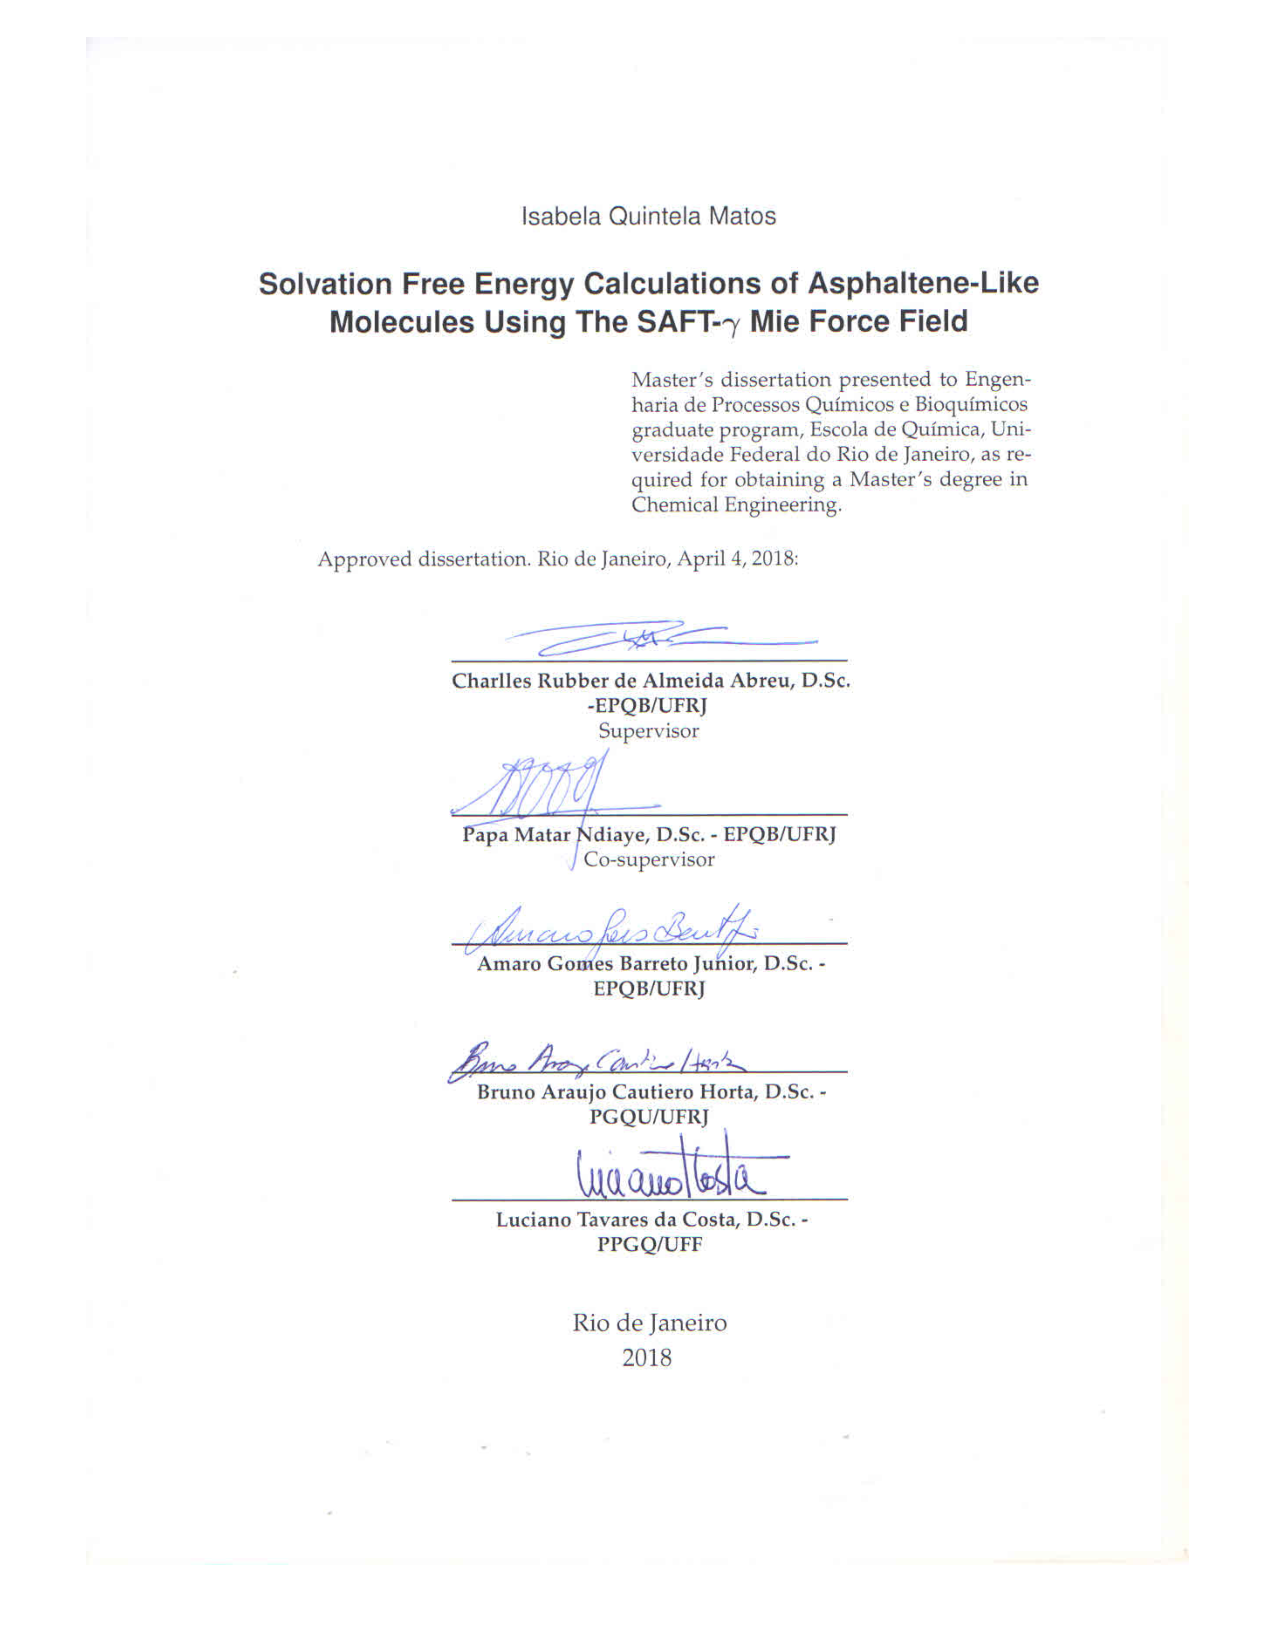
\includepdf{aprovada.pdf}
\DIFaddend %
\DIFdelbegin %DIFDELCMD < \begin{folhadeaprovacao}
%DIFDELCMD < 

%DIFDELCMD <   \begin{center}
%DIFDELCMD <     {\ABNTEXchapterfont\large\imprimirautor}
%DIFDELCMD < 

%DIFDELCMD <     \vspace*{\fill}\vspace*{\fill}
%DIFDELCMD <     \begin{center}
%DIFDELCMD <       \ABNTEXchapterfont\bfseries\Large\imprimirtitulo
%DIFDELCMD <     \end{center}
%DIFDELCMD <     \vspace*{\fill}
%DIFDELCMD <     

%DIFDELCMD <     %%%
\DIFdel{\hspace{.45\textwidth}
    }%DIFDELCMD < \begin{minipage}{.5\textwidth}
%DIFDELCMD <         \imprimirpreambulo
%DIFDELCMD <     \end{minipage}%%%
\DIFdelend %DIF > \begin{folhadeaprovacao}
%
\DIFdelbegin %DIFDELCMD < \vspace*{\fill}
%DIFDELCMD <    \end{center}
%DIFDELCMD <         

%DIFDELCMD <    %%%
\DIFdel{Approved dissertation. }%DIFDELCMD < \imprimirlocal%%%
\DIFdel{, April 4, 2018:
}%DIFDELCMD < 

%DIFDELCMD <    \assinatura{\textbf{Charlles Rubber de Almeida Abreu, D.Sc. -EPQB/UFRJ} \\ Supervisor} 
%DIFDELCMD <    \assinatura{\textbf{Amaro Gomes Barreto Junior, D.Sc. - EPQB/UFRJ} \\ Guest 1}
%DIFDELCMD <    \assinatura{\textbf{Bruno Araujo Cautiero Horta, D.Sc. - PGQU/UFRJ} \\ Guest 2}
%DIFDELCMD <    \assinatura{\textbf{Luciano Tavares da Costa, D.Sc. - PPGQ/UFF} \\ Guest 3}
%DIFDELCMD <       

%DIFDELCMD <    \begin{center}
%DIFDELCMD <     \vspace*{0.5cm}
%DIFDELCMD <     {\large\imprimirlocal}
%DIFDELCMD <     \par
%DIFDELCMD <     {\large\imprimirdata}
%DIFDELCMD <     \vspace*{1cm}
%DIFDELCMD <   \end{center}
%DIFDELCMD <   

%DIFDELCMD < \end{folhadeaprovacao}
%DIFDELCMD < %%%
\DIFdelend %DIF >   \begin{center}
%DIF >     {\ABNTEXchapterfont\large\imprimirautor}
%DIF > 
%DIF >     \vspace*{\fill}\vspace*{\fill}
%DIF >     \begin{center}
%DIF >       \ABNTEXchapterfont\bfseries\Large\imprimirtitulo
%DIF >     \end{center}
%DIF >     \vspace*{\fill}
%DIF >     
%DIF >     \hspace{.45\textwidth}
%DIF >     \begin{minipage}{.5\textwidth}
%DIF >         \imprimirpreambulo
%DIF >     \end{minipage}%
%DIF >     \vspace*{\fill}
%DIF >    \end{center}
%DIF > 
%DIF >    Approved dissertation. \imprimirlocal, April 4, 2018:
%DIF >     \vspace*{-0.5cm}
%DIF >    \assinatura{\textbf{Charlles Rubber de Almeida Abreu, D.Sc. -EPQB/UFRJ} \\ Supervisor} 
%DIF >    \assinatura{\textbf{Papa Matar Ndiaye, D.Sc. -EPQB/UFRJ} \\ Co-Supervisor} 
%DIF >    \assinatura{\textbf{Amaro Gomes Barreto Junior, D.Sc. - EPQB/UFRJ} \\ Guest 1}
%DIF >    \assinatura{\textbf{Bruno Araujo Cautiero Horta, D.Sc. - PGQU/UFRJ} \\ Guest 2}
%DIF >    \assinatura{\textbf{Luciano Tavares da Costa, D.Sc. - PPGQ/UFF} \\ Guest 3}
%DIF >       
%DIF >    \begin{center}
%DIF >     \vspace*{0.2cm}
%DIF >     {\large\imprimirlocal}
%DIF >     \par
%DIF >     {\large\imprimirdata}
%DIF >     \vspace*{0.5cm}
%DIF >   \end{center}
%DIF >   
%DIF > \end{folhadeaprovacao}
% ---

% ---
% Dedicatória
% ---
%\begin{dedicatoria}
%   \vspace*{\fill}
%   \centering
%   \noindent
%   \textit{ Este trabalho é dedicado às crianças adultas que,\\
%   quando pequenas, sonharam em se tornar cientistas.} \vspace*{\fill}
%\end{dedicatoria}
% ---

% ---
% Agradecimentos
% ---
\begin{agradecimentos}
I would like to give some words of thanks to my parents for the support during my relocation from Aracaju to Rio de Janeiro, and for supporting my decisions. I also would like to thank my adviser Charlles Rubber de Almeida Abreu for the elucidative meetings and for taking the time to explain in such clear way the concepts of molecular simulations and free energy calculations. To my co-adviser Papa Matar Ndiaye, I would like to thank for presenting the ATOMS group to me and for accepting my participation in his project about asphaltenes. I also would like to thank all the ATOMS group members, especially Ana Jorgelina Silveira  for helping me with any theoretical and software doubts I had. Finally, I would like to thank Cenpes/Petrobras (project code: 17.564) for the financial support. 
\end{agradecimentos}
% ---

% ---
% Epígrafe
% ---
%\begin{epigrafe}
%    \vspace*{\fill}
%	\begin{flushright}
%		\textit{"A wizard is never late, nor is he early, he arrives precisely when he means to."
%		(Peter Jackson).}
%	\end{flushright}
%\end{epigrafe}
% ---

% ---
% RESUMOS
% ---

% resumo em português
\setlength{\absparsep}{18pt} % ajusta o espaçamento dos parágrafos do resumo
%\begin{resumo}
% Segundo a \citeonline[3.1-3.2]{NBR6028:2003}, o resumo deve ressaltar o
% objetivo, o método, os resultados e as conclusões do documento. A ordem e a extensão
% destes itens dependem do tipo de resumo (informativo ou indicativo) e do
% tratamento que cada item recebe no documento original. O resumo deve ser
% precedido da referência do documento, com exceção do resumo inserido no
% próprio documento. (\ldots) As palavras-chave devem figurar logo abaixo do
% resumo, antecedidas da expressão Palavras-chave:, separadas entre si por
% ponto e finalizadas também por ponto.
%
% \textbf{Palavras-chave}: latex. abntex. editoração de texto.
%\end{resumo}
% resumo em inglês
\begin{resumo}[Abstract]
 \begin{otherlanguage*}{english}
   Asphaltenes are a  relevant fraction of crude oil to the oil industry since they can precipitate during the oil processing. Hence, we, at this dissertation, studied the solvation free energies of molecules mimicking asphaltenes in different solvents with a coarse-grained model known as SAFT-$\gamma$ Mie force field. We obtained solvation free energies  by carrying out molecular dynamics simulations using the expanded ensemble method. The output of these simulations was then used to estimate the solvation free energies. For this, we employed the MBAR method. The results with solvents other than water had low absolute deviations from experimental data. In turn, hydration free energy calculations required a binary interaction parameter estimated with output data from molecular dynamics in order to obtain accurate free energy differences. These results indicated problems on the description of the water molecule by the SAFT-$\gamma$ Mie force field, but, generally, proved that this coarse-grained model could represent the solvation free energies of the studied solute-solvent pairs.

   \vspace{\onelineskip}

   \noindent 
   \textbf{Keywords}: Solvation free energy. Asphaltenes. SAFT-$\gamma$ Mie force field.
 \end{otherlanguage*}
\end{resumo}

% ---
% inserir lista de ilustrações
% ---
\pdfbookmark[0]{\listfigurename}{lof}
\listoffigures*
\cleardoublepage
% ---

% ---
% inserir lista de tabelas
% ---
\pdfbookmark[0]{\listtablename}{lot}
\listoftables*
\cleardoublepage
% ---

% ---
% inserir lista de símbolos
% ---
\begin{simbolos}
  \item[$T$] Temperature
  \item[$P$] Pressure
  \item[$V$] Volume
  \item[$t$] Time
  \item[$p$] Momentum
  \item[$r$] Coordinates
  \item[$U,u$] Potential energy
  \item[$u$] Potential energy at reduced units
  \item[$m$] Mass
  \item[$v$] Velocity
  \item[$P$] Pressure
  \item[$ \mathcal{H} $] Hamiltonian
  \item[$q$] Generalized coordinates
  \item[$K $] 	Kinetic energy 
  \item[$N$] Number of atoms/molecules
  \item[$h$] Planck constant
  \item[$S$] Entropy
  \item[$\kappa_{b}$] Boltzmann constant
  \item[$\beta$] $1/\kappa_{b}T$
  \item[$\mu$] Chemical potential
  \item[$A$] Helmholtz free energy
  \item[$G$] Gibbs free energy
  \item[$f$] Free energy at reduce units
  \item[$F$] Forces
  \item[$\epsilon$] Depth of the potential well
  \item[$\sigma$] Distance corresponding to a zero intermolecular potential
  \item[$\lambda _{r}$] Repulsive exponent
  \item[$\lambda _{a}$] Attractive exponent
  \item[$x_{i}$] Molar fraction 
  \item[$w_{i}$] Weight fraction 
  \item[$\rho$] Density
  \item[$\lambda$] Coupling parameter 
  \item[$\eta$] Arbitrary weight 
  \item[$k_{ij}$] Binary interaction parameter
\end{simbolos}
% ---

% ---
% inserir o sumario
% ---
\pdfbookmark[0]{\contentsname}{toc}
\tableofcontents*
\cleardoublepage
% ---



% ----------------------------------------------------------
% ELEMENTOS TEXTUAIS
% ----------------------------------------------------------



% ----------------------------------------------------------
% Introdução (exemplo de capítulo sem numeração, mas presente no Sumário)
% ----------------------------------------------------------
\clearpage
\setcounter{page}{1}
\chapter{Introduction} % Main chapter title
\label{Chapter1} % 
\pagestyle{simple}
\onehalfspacing
Solvation free energy calculations with molecular dynamics (MD) have a variety of applications ranging from drug design in the pharmaceutical industry to the development of separation technologies in the chemical industry. {Solvation free energy is, more specifically, the difference in free energy related to the process of transferring a solute from an ideal gas phase into a liquid solution \cite{shirts2013}}. Through the study of the solvation phenomenon, it is possible to obtain information about the behavior of the solvent in different thermodynamic conditions and the influence of the solute's molecular geometry. It is also possible to calculate other important properties with the solvation free energy, namely the activity coefficient at infinite dilution, Henry constant, and partition coefficients.{ Additionally, solvation free energy calculations can be part of the methodology of calculating solubility from molecular dynamics}. 

The solvation free energy calculations described above are intrinsically complex due to the many competing forces interfering in the behavior of the solute-solvent interaction. \DIFdelbegin \DIFdel{In addition}\DIFdelend \DIFaddbegin \DIFadd{Also}\DIFaddend , free energy simulations are susceptible to sampling problems in low energy regions, and simulation results need to be correctly post-processed in order to yield free energy differences with small uncertainties. {Another influencing factor in the output of these calculations is the choice of force field used to model the solvent and solute molecules. Force field is the name given to the group of parameters and equations used to represent the potential energy function of a system in molecular simulations. They have different levels of description, such as quantum mechanics, atomistic, and coarse-grained. The quantum mechanics approach describes the motion of electrons and requires for the solution of the Schr\"{o}dinger equation during the simulation. In the atomistic description, only the atomic motions are represented,  and this is done by solving Newton's equations of motion. Finally, in the coarse-grained description, atoms are grouped into pseudo-atoms or beads, and the equations of motion are solved for them. 

	These coarse-grained models are generally able to reproduce experimental free energy differences since the effects of reducing degrees of freedom in the entropy are counterbalanced by the reduction of enthalpic terms \cite{kmiecik2016}. This fact makes these models a viable option to decrease the computational time of solvation free energy calculations. Additionally, deficiencies in the description of small molecules by coarse-grained models can be revealed by free energy calculations \cite{mobley2007,shirts2013}. Hence, we, in this study, assess the performance and shortcomings of the SAFT-$\gamma$ Mie coarse-grained force field  \cite{avendano2011} with free energy calculations of a variety of solute-solvent pairs. We choose this coarse-grained force field because it uses, unlike the majority of the force fields, the Mie potential \cite{MIE} and because its method of obtaining parameters is more straightforward than those of other \DIFaddbegin \DIFadd{coarse-grained }\DIFaddend models. It was initially parameterized with pure component equilibrium and interfacial tension data \cite{avendano2011}, and this strategy has provided satisfactory results. Examples include the prediction of phase equilibrium of aromatic compounds \cite{muller2017}, alkanes, light gases \cite{herdes2015}, and water \cite{lobanova2015}, thermodynamic properties of carbon dioxide and methane \cite{cassiano1}, multiphase equilibrium of mixtures of water, carbon dioxide, and n-alkanes \cite{lobanova2016}, and water/oil interfacial tension \cite{herdes2017}.} 


We selected the solvents and solutes in our free energy calculations with the intention of testing the force field with standard sets used as a benchmark in solvation free energy calculations and with polycyclic aromatic substances used as models to asphaltenes. Asphaltenes are complicated to characterize by determining their composition on a molecular basis, but the literature broadly accepts that they can be described as a fraction of crude oil soluble in toluene and insoluble in n-alkanes (pentane, hexane, heptane) \cite{SJOBLOM2003399}. They have motivated many studies with interest in developing models for their structure and behavior due to all the problems they can cause during their transportation and refining such as precipitation during the oil processing \cite{SJOBLOM20151}. This precipitation issue is a recurrent problem due to the growing market of the production of crude oil in deep waters, whose conditions are favorable to precipitation \cite{AIC:AIC10243}. As an example, asphaltene precipitation due to pressure drop can clog oil production equipment and cause a growth in the cost of production \cite{doi:10.1021/ef010047l}. All these factors make the understanding of the behavior of asphaltenes in different chemical and physical environments relevant to the oil industry. 

As said in the previous paragraph, asphaltene characterization still faces some issues. Hence, we choose to use polycyclic aromatic hydrocarbons (PAHs), which have well-defined characteristics, to initially test the efficiency of the SAFT-$\gamma$ Mie force field in describing the solvation phenomenon. PAHs are a group of organic compounds that have fused rings, carbon and hydrogen in their structure \cite{RAVINDRA20082895}\DIFaddbegin \DIFadd{, which are characteristic shared with asphaltenes}\DIFaddend . The ones utilized in this work were phenanthrene, anthracene, and pyrene since they share similarities with asphaltenes regarding their solubility. In this context,  we selected compounds that are used to characterize asphaltenes (toluene, hexane) as solvents in our free energy calculations. We also tested the anti-solvent/solvent effect of carbon dioxide due to its influence in asphaltene precipitation during the oil processing \cite{SOROUSH2014405}. \DIFdelbegin \DIFdel{With these calculations of solvation free energies with the SAFT-$\gamma$ Mie model, we intend to improve this force field and provide satisfactory solvation free energy estimates of PAHs with a coarse-grained model. The }\DIFdelend \DIFaddbegin \DIFadd{Hence, the }\DIFaddend success of the description
of \DIFaddbegin \DIFadd{solvation free energies of }\DIFaddend small asphaltene-like compounds by this force field can then open up the possibility of obtaining satisfactory results for more complex asphaltene models with a force field with a low computational cost.

\DIFaddbegin \section{Objectives} %DIF >  Main chapter title

\DIFadd{The general objective of this dissertation is to acquire reasonable estimates of the solvation free energies of PAHs, which can represent asphaltenes, using molecular dynamics simulations with the SAFT-$\gamma$ Mie force field. By doing that, we intend to provide information about the solvation phenomenon of an extremely important compound for the oil industry. 
}

\DIFadd{The specific objectives are to :
}

 \begin{description} [1.5cm]
	\item[$\bullet$] \DIFadd{Estimate the parameters of the SAFT-$\gamma$ Mie force field for phenanthrene using the two available strategies for the parameterization of aromatic molecules with this force field. 
	}\item[$\bullet$] \DIFadd{Estimate the binary interaction parameter required by the SAFT-$\gamma$ Mie force field for aqueous mixtures.
	}\item[$\bullet$] \DIFadd{Optimize the parameters necessary to carry out the expanded ensemble simulations.
	}\item[$\bullet$] \DIFadd{Carry out expanded ensemble simulations to obtain the potential energies using a thermodynamic path and a softcore model for the potential energy function.
	}\item[$\bullet$] \DIFadd{Estimate the solvation free energies with the Multistate Bennett Acceptance (MBAR) method using the potential energies obtained with molecular dynamics simulations.
	}\item[$\bullet$] \DIFadd{Calculate the partition coefficients for some systems studied here using the estimated solvation free energies.
} \end{description} 
\DIFaddend % Chapter Template

\chapter{Literature Review} % Main chapter title
%\doublespacing
\label{Chapter2} % Change X to a consecutive number; for referencing this chapter elsewhere, use \ref{ChapterX}
\section{Molecular Simulations of Asphaltene-Like Molecules}

Asphaltenes, unlike other petroleum fractions, are not defined on a molecular basis. The most accepted definition is that they are a fraction of crude oil insoluble in n-alkanes (pentane, hexane, and heptane) and soluble in toluene \cite{SJOBLOM2003399}. Due to uncertainties related to their structures, much work has been done to develop model compounds that have a well-defined structure and can represent asphaltenes. The two categories of models presented in the literature are the archipelago and continental models. In the archipelago model, asphaltenes consist of polyaromatic parts linked together by aliphatic or naphthenic moieties and, in the continental model, they consist of a single
polyaromatic ring with linked aliphatic or naphthenic chains \cite{doi:10.1021/ef900975e,doi:10.1080/0892702031000148762}. The choice of the model's structure \DIFdelbegin \DIFdel{, such as chemical bonding, }\DIFdelend is highly essential since some structures\DIFaddbegin \DIFadd{/ arrangements }\DIFaddend can cause the occurrence of high-energy regions during the simulation \cite{doi:10.1021/ef200507c} .   

In order to evaluate the strengths and shortcomings of asphaltene models, articles have been published about the calculations of their properties. There is an agreement in studies of these models with molecular simulation, such as the influence of the model in the packing tendency of the molecule \cite{doi:10.1080/10298436.2011.575141}. \citeonline {doi:10.1021/ef9004576} utilized molecular dynamics in the study of the nanoaggregation of four types of model asphaltene molecules (continental, Violanthrone-79, anionic continental, and thiophenic anionic continental) in binary mixtures of toluene and water. The authors observed that, in thin films of toluene trapped between two aqueous phases, both interface-bound and core-bound asphaltenes have similar diffusion behavior. \citeonline{doi:10.1021/acs.energyfuels.6b02161} reported molecular dynamics simulations of four model asphaltenes, including archipelago and continental model. They alleged that there is no formation of nanoaggregates and that the distribution of asphaltene clusters is continuous for mixtures of asphaltenes in heptane. 

Molecular dynamics simulations were also utilized in the study of \citeonline{ervik20162}  to obtain the correct interfacial orientation of asphaltenes using a coarse-grained model of the interface and the asphaltene molecules. Also using a coarse-grained force field, \citeonline{doi:10.1021/ef502209j} carried out molecular simulations with a continental asphaltene model. The results reproduced experimental data of aggregation
of asphaltene molecules in n-heptane and solubility in toluene. \citeonline{doi:10.1021/ef5020428} performed a molecular
dynamics study with the GROMOS 45a3 force field \cite{JCC:JCC1078} to identify the influence of the structural characteristics of different asphaltene molecules.

\citeonline{doi:10.1021/ef301610q} employed the archipelago model in their work to investigate the interfacial behavior of asphaltene molecules at the oil-water interface using molecular dynamics simulations with the OPLS-AA force field \cite{doi:10.1021/ja00214a001}. They found that asphaltenes are preferably distributed in the oil phase in the case of pure toluene and at the oil-water interface
in the case of pure heptane. They also discovered an
oscillatory behavior of asphaltene molecules at the oil-water interface when using the archipelago model. \citeonline{doi:10.1021/jp407363p} used a perylene-based model to study molecular association and interaction as well as the adsorption properties of the perylene molecule at the water/toluene or water/heptane interface. 

\section{Coarse-Grained (CG) Force Fields}\label{cgff}


Molecular simulations, as those described in the previous section, can be carried out at different levels of description. The detailed atomistic level or \textit{ab initio} level is described by the laws of quantum mechanics. The system consists of a set of subatomic particles in which \DIFaddbegin \DIFadd{the }\DIFaddend Schr\"{o}dinger's equation is solved for all of them. The next level is the atomistic description. \DIFdelbegin \DIFdel{It considers that the system is made up of atoms following the laws }\DIFdelend \DIFaddbegin \DIFadd{In this description, the equations }\DIFaddend of classical mechanics \DIFaddbegin \DIFadd{are solved for the atoms in the system}\DIFaddend .  Force fields at this level are based on van der Waals interactions, which may include neutral or Coulombic charged sites. \DIFaddbegin \DIFadd{The polarizability effect may also be accounted by some force fields. }\DIFaddend Contributions due to intramolecular interactions such as bond-stretching, angle-bending, and torsion are also \DIFdelbegin \DIFdel{usually accounted for }\DIFdelend \DIFaddbegin \DIFadd{considered }\DIFaddend in these kinds of force fields. When the simulation scale needs to be increased, and the atomistic simulations become too computationally expensive such as in the study of biological systems, the coarse-grained (CG) description \DIFdelbegin \DIFdel{is more suited. It }\DIFdelend \DIFaddbegin \DIFadd{can be an alternative to decrease the computational cost. This description }\DIFaddend considers that the system is made up of pseudo-atoms or beads \DIFdelbegin \DIFdel{that contain }\DIFdelend \DIFaddbegin \DIFadd{representing }\DIFaddend multiple atoms or even an entire molecule. 

There is an evident loss of information in grouping atoms; hence it is necessary to guarantee that the process of eliminating unnecessary or unimportant information ('coarse-graining') does not affect the system's physical behavior. Ideally, coarse-grained models need to have representability, robustness, transferability, and computational efficiency. Representability means that we can use a model at a state point other than the one in which it was parameterized. The other characteristic, robustness, is related to the model's ability to enable reliable predictions for various structural, thermodynamic, or transport properties. Finally, a transferable model is one in which the representation of atomic or chemical moieties have the same behavior in different molecules- e. g., a pseudo-atom representing $CH_{2}$ should have the same characteristics both in an alkene molecule and in a polyethylene molecule     \cite{doi:10.1146/annurev-chembioeng-061312-103314}. To achieve the cited goals, coarse-grained force fields are usually developed by mapping the atomistic model to define the pseudo-atoms, which are generally formed by similar functional groups. 

The level of coarse-graining also needs to be established. \DIFdelbegin \DIFdel{\mbox{%DIFAUXCMD
\citeonline{hadley2012} }%DIFAUXCMD
affirm that a maximum of six heavy atoms (non-hydrogen atoms ) per bead are traditionally used in order to not lose valuable details and to maintain isotropic representations of the beads}\DIFdelend \DIFaddbegin \DIFadd{The decision of the number of atoms per bead should be careful. There is a compromise between accuracy and computational efficiency since the simulations become faster when we group more atoms per bead, but the results can lose accuracy}\DIFaddend . After the mapping, CG force fields need to be parametrized. There are two different approaches, \DIFdelbegin \DIFdel{bottom up }\DIFdelend \DIFaddbegin \DIFadd{bottom-up }\DIFaddend and top-down, to link the simulations on the coarse-grained scale to another scale, schematically represented in \figref{fig:multiscale}. The bottom-up approach uses information of a more detailed scale such as the quantum mechanics description or the atomistic description to obtain information necessary to the parametrization. This method highly depends on the quality of the more detailed model to succeed. In the top-down methodology, one obtains parameters from larger scales, namely experimental thermodynamic or transport properties. 

\begin{figure}[H]
	\raggedleft
	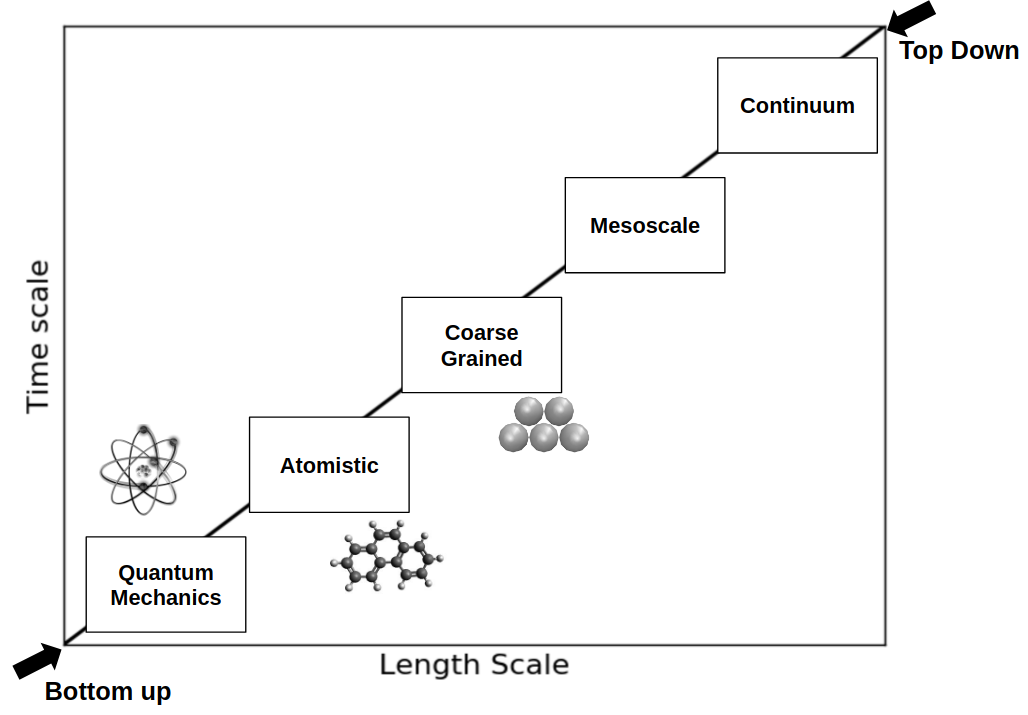
\includegraphics[width=0.9\textwidth]{Figures/multiscale}
	\caption{Schematic representation of the two approaches of coarse-graining.}
	\label{fig:multiscale}
\end{figure}
\FloatBarrier

One of the first applications of coarse-grained models was in the study of protein folding \cite{levitt1975,levitt1976}. These earlier protein CG models were based on known molecular structure, and they \DIFdelbegin \DIFdel{contributed }\DIFdelend \DIFaddbegin \DIFadd{did not represent the properties of proteins correctly, but they gave an initial contribution }\DIFaddend to the knowledge of physicochemical forces associated with protein folding and protein interactions \cite{koga2001}. More recently, models were developed focusing on retaining the protein's chemical specificity. The Bereau and Deresno model \cite{bereau2009} represents a single amino acid residue with a maximum of four beads, and it was used in studies of protein folding and aggregation. However, this model still needs tuning to improve protein stability \cite{bereau2010}. The OPEP (Optimized Potential for Efficient Protein Structure Prediction) model \cite{opep2014,opep2015} represents a single amino acid with a maximum of six beads. It was used to investigate a variety of phenomena, ranging from protein folding to the modeling of DNA-RNA complexes \cite{opep2011,opep2009,opep2014}. Other CG protein models used in the literature are the SCORPION (solvated coarse-grained protein interaction)  \cite{scorpion2013}, the UNRES (United Residue) \cite{unres2014} and the MARTINI model \cite{martini2013}. The latter one is the most popular model for CG modeling of membrane proteins \cite{martini20132}. \DIFaddbegin \DIFadd{Although these models are widely used, the existing coarse-grained force fields utilized to model proteins still need improvement, since the efficient use of coarse-grained models for proteins usually requires rigorous reconstruction of the atom-level representation, and this has only been possible for some moderate resolution coarse-grained models  \mbox{%DIFAUXCMD
\cite{kmiecik2016}}%DIFAUXCMD
.
}

\DIFaddend The MARTINI force field is also extensively used as a CG model for water. This force field represents four water molecules as one bead using a shifted Lennard-Jones potential. Despite its extensive use, the MARTINI water model does not \DIFdelbegin \DIFdel{properly }\DIFdelend \DIFaddbegin \DIFadd{correctly }\DIFaddend reproduce properties such as interfacial tension and compressibility \cite{shinoda2010}. Besides, it can freeze at room temperature \cite{winger2009,martini2007}, which requires the use of \DIFdelbegin \DIFdel{anti-freeze }\DIFdelend \DIFaddbegin \DIFadd{anti-freezing }\DIFaddend agents during the simulations. This behavior can be explained by the high level of coarse-graining (4:1), the lack of explicit charges, and the use of a 12-6 potential. \DIFdelbegin \DIFdel{\mbox{%DIFAUXCMD
\citeonline{chiu2010} }%DIFAUXCMD
used the Morse Potential, which is softer than the LJ potential, to improve the MARTINI model. }\DIFdelend \citeonline{shinoda2007} used different forms of the Mie potential to build a versatile and transferable coarse-grained model for surfactant/water systems using density, interfacial tension, and hydration free energies (solvation free energies in water) data. In this model, three water molecules are represented by one pseudo-atom, and the water cross interactions are represented by a 12-4 Mie potential, and the surfactant (alkanes, oxyethylenes, ethylene glycols, ethers, and alcohols) interactions are represented by a 9-6 Mie potential. \DIFaddbegin \DIFadd{\mbox{%DIFAUXCMD
\citeonline{chiu2010} }%DIFAUXCMD
used another type of intermolecular potential, the Morse Potential, which is softer than the LJ potential, to improve the MARTINI model. 
}\DIFaddend 

Outside of the MARTINI framework, \DIFaddbegin \DIFadd{\mbox{%DIFAUXCMD
\citeonline{shinoda2010} }%DIFAUXCMD
studied different levels of coarse-graining for water ranging from one to four molecules per bead using different Mie and Morse potentials. Other investigations also assessed the use of soft-core potentials to study aqueous solutions of surfactants \mbox{%DIFAUXCMD
\cite{shinoda2007}}%DIFAUXCMD
, as well as ionic liquids \mbox{%DIFAUXCMD
\cite{bhargava2009}}%DIFAUXCMD
, lipids \mbox{%DIFAUXCMD
\cite{shinoda20102}}%DIFAUXCMD
, and membranes \mbox{%DIFAUXCMD
\cite{pantano2009}}%DIFAUXCMD
. \mbox{%DIFAUXCMD
\citeonline{doi:10.1063/1.3553378} }%DIFAUXCMD
also developed a coarse-grained water model for the GROMOS model using a systematic analysis of different properties of small water clusters. According to their analysis, the best representation of water is achieved when one bead represents five water molecules. In this model, the potential energy is calculated using the Lennard-Jones potential, and electrostatic interactions are explicitly considered. }\DIFaddend \citeonline{10.1371/journal.pone.0028637} proposed the ELBA coarse-grained model for molecular dynamics simulations of lipid membranes. In this model, electrostatics are modeled explicitly by point charges, and \DIFdelbegin \DIFdel{water molecules are }\DIFdelend \DIFaddbegin \DIFadd{one water molecule is }\DIFaddend represented by a single Lennard-Jones bead embedded with a point dipole. \citeonline{doi:10.1021/acs.jctc.5b00963} expanded the ELBA force field to model 1-hexanol, 1-nonanol, n-hexane, and n-nonane by representing three carbons with a single bead. \DIFdelbegin \DIFdel{Using different Mie and Morse potentials, \mbox{%DIFAUXCMD
\citeonline{shinoda2010} }%DIFAUXCMD
studied different levels of coarse-graining for water ranging from one to four molecules per bead. Other investigations also assessed the use of soft-core potentials to study aqueous solutions of surfactants \mbox{%DIFAUXCMD
\cite{shinoda2007}}%DIFAUXCMD
, as well as ionic liquids \mbox{%DIFAUXCMD
\cite{bhargava2009}}%DIFAUXCMD
, lipids \mbox{%DIFAUXCMD
\cite{shinoda20102}}%DIFAUXCMD
, and membranes \mbox{%DIFAUXCMD
\cite{pantano2009}}%DIFAUXCMD
. }\DIFdelend Another CG model for water based on the Mie Potential is the SAFT-$\gamma$ Mie force field \cite{lobanova2015}. In this strategy, there are two different models: CGW1-vle and CGW1-ift. Both of them represent \DIFdelbegin \DIFdel{the }\DIFdelend \DIFaddbegin \DIFadd{one }\DIFaddend water molecule as one bead, and the Mie Potential has a repulsive and an attractive exponent equal to 8 and 6, respectively. The CGW1-vle model was parameterized using saturated-liquid density and vapor pressure data and should be used for simulations of aqueous systems in fluid-phase equilibrium at high temperatures and pressures. This model still suffers from premature freezing with a triple point at 343 K. The other model, CGW1-ift, was parameterized using saturated-liquid density and interfacial tension data. Hence, it is best suited for interfacial property calculations. Both models had temperature-dependent size and energy parameters and performed well for these properties over the entire liquid temperature range. The SAFT-$\gamma$ Mie force field has also been applied to other compounds with satisfactory results. \citeonline{muller2017} parameterized the force field for aromatic compounds and tested it with simulations of fluid phase equilibrium. \citeonline{herdes2015} carried out simulations of alkanes and light gases. \citeonline{lobanova2016} tested the force field with binary and ternary mixtures of water and carbon dioxide. There are also articles with the SAFT-$\gamma$ Mie being used for computing thermodynamic and transport properties of carbon dioxide and methane \cite{cassiano1,cassiano2} and water/oil interfacial tension \cite{herdes2017}.  

\section{Solvation Free Energies}

Solvation free energy calculations with molecular dynamics can be used to evaluate the quality of a coarse-grained force field, such as the models described in the preceding section, since these estimations can reveal deficiencies in a force field. Besides this application, solvation free energies are used to obtain information about the behavior of the solvent in different thermodynamic conditions and to assess the influence of the solute's molecular geometry on the solvation phenomenon. Due to their range of application and inherent complexity, free energy calculations were the subject of a variety of studies in the last decades interested in improving the free energy simulations and their post-processing methods \cite{mbar,bareva,dexp,gdel}.

Recent articles \cite{PMID:24928188,mobley2017} made available a large database of hydration free energies of small molecules using the GAFF force field for the
solutes and the TIP3P model for water. \citeonline{Beckstein2014} also calculated the hydration free energies for fifty-two compounds with the OPLS-AA force field. They obtained an overall root mean square deviation from the experimental data of 1.75 kcal/mol and concluded that the reproducibility of the Lennard-Jones parameters is the main constraint of the precision of their results. \citeonline{izairi2017} also studied hydration free energies but with the intention of comparing the polar and nonpolar contributions. Garrido \textit{et al.} (2009, 2011) calculated the free energy of solvation of large alkanes in 1-octanol and water with three different force fields (TraPPE, GROMOS, and OPLS-AA/TraPPE). These authors also estimated the solvation free energy of propane and benzene in non-aqueous solvents like n-hexadecane, n-hexane, ethylbenzene, and acetone with the united atoms TraPPE force field (TraPPE-UA) and the all-atoms TraPPE force field (TraPPE-AA). \citeonline{roy2017} addressed the choice of the Lennard-Jones parameters for predicting solvation free energy of different solutes in 1-octanol. They calculated the solvation free energy of a set of 205 small organic molecules in 1-octanol and found that the force field parametrization of n-octanol proposed by \citeonline{doi:10.1063/1.2972978} provided the best agreement to the experimental data. \citeonline{goncalves} calculated the free energy of solvation using the polarizable continuum model coupled to molecular dynamics simulation with the GROMOS force field. These calculations were done with a representative set of solutes and with the solvents tetrachloride, chloroform, and benzene. Using the GAFF and the polarizable AMOEBA force fields, \citeonline{mohamed2016} evaluated the solvation free energy of small molecules in toluene, chloroform, and acetonitrile, and obtained a mean unsigned error of 1.22 kcal/mol for AMOEBA and 0.66 kcal/mol for GAFF. To define the role of water as the solvent in the docking structure determination of proteins, \citeonline{MATUBAYASI201745} developed a method to compute the solvation free energy of proteins while using OPLS-AA force field for the
solutes and the TIP3P model for water. \citeonline{doi:10.1021/acs.jctc.5b00963} expanded the ELBA force field to calculate solvation free energies of more than 150 solutes taken from the Minnesota solvation
database in polar (water, hexanol, octanol, and nonanol) and apolar (hexane, octane, and nonane) solvents. He obtained mean absolute deviations of 1 kcal/mol for water and 1.5 kcal/mol for hexane. In this model, three carbons are represented by a single bead and water is also represented by a single bead. 

Despite the variety of data using the intramolecular Lennard-Jones potential, there are not many studies with the Mie Potential in free energy calculations. That is why we, in the present study, try to provide information about these predictions with the SAFT-$\gamma$ Mie coarse-grained force field.  As said before, the output of these calculations are highly dependent on the force field, and some coarse-grained models produced satisfactory results for these simulations. In addition\DIFdelbegin \DIFdel{to that}\DIFdelend , the use of a coarse-grained model can decrease the simulation time, as explained in Section \ref{cgff}. Therefore, the \DIFdelbegin \DIFdel{discovery }\DIFdelend \DIFaddbegin \DIFadd{consideration }\DIFaddend of other coarse-grained approaches with similar performances to the all-atoms force fields can help increase the scale of solvation free energy calculations. 

\section{Solvation Free Energy Calculation Methods}\label{SFECM}

Solvation free energy calculations account for the difference in free energy related to transferring the solute from the ideal gas phase to the liquid solvent phase. To do that, we gradually insert the solute in the solvent. This process is mathematically carried out by using a coupling parameter ($\lambda$) on the total potential energy function, where $\lambda$ represents the intermediate states in the transition from the solute in the ideal gas phase ($\lambda=0$) to the solute entirely inserted in the solvent phase ($\lambda = 1$). Hence,  during the solvation free energy simulations, we obtain total potential energies corresponding to these coupling parameters [($U(\lambda)$]. After the simulations, these potential energies need to be post-processed and analyzed \DIFdelbegin \DIFdel{for us }\DIFdelend \DIFaddbegin \DIFadd{so as }\DIFaddend to calculate the solvation free energies efficiently. \DIFaddbegin \DIFadd{Therefore, in this section, we present a quick review of the methods available in the literature to perform the estimation of the solvation free energies. }\DIFaddend Since these calculations can have slow convergence, many \DIFaddbegin \DIFadd{scientific groups }\DIFaddend in the last decades focused on developing analysis methods to \DIFdelbegin \DIFdel{calculate }\DIFdelend \DIFaddbegin \DIFadd{estimate these }\DIFaddend free energies. Almost all of these methods rely on the following approaches:   thermodynamic integration, histograms, and free energy perturbation (FEP) based methods.

\subsection{Thermodynamic integration}

The thermodynamic integration method \cite{kirkwood1935} uses equilibrium averages to evaluate the energy derivative with respect to the coupling parameter ($\lambda$): 
%Then, the free energies are calculated by  doing the derivative ($\frac{\partial G}{\partial \lambda} $):
%
%\begin{equation}
%\label{eq:ti1}
%\begin{aligned}
%\frac{\partial \beta G}{\partial \lambda} = - \frac{1}{Z (\lambda)}\frac{\partial Z}{\partial \lambda}
%\end{aligned}
%\end{equation}
%
%The Eq. \eqref{eq:dif} can be rewritten according to the Halmitonian of the system ($\mathcal{H}$):
%
%\begin{equation}
%\label{eq:ti2}
%\begin{aligned}
%\Delta G = - \kappa_{b}T ln \left( \frac{Z_{1}}{Z_{0}}\right) = -\kappa_{b}T ln \int \frac{exp(-\beta \mathcal{H} _{1}(r,p)) dr dp}{exp(-\beta \mathcal{H} _{0}(r,p)) dr dp}
%\end{aligned}
%\end{equation}

%Substituting Eq. \eqref{eq:ti2} in \eqref{eq:ti2} and adding the coupling parameter to the Halmitonian ($\mathcal{H} (r,p,\lambda)$) in order to describe the transition between the end states:

%\begin{equation}
%\label{eq:ti3}
%\begin{aligned}
%\frac{\partial \beta G}{\partial \lambda} =  \int \frac{\frac{\partial \mathcal{H} (r,p,\lambda)}{\partial \lambda}exp(-\beta \mathcal{H}(r,p,\lambda)) dr dp}{exp(-\beta \mathcal{H}(r,p,\lambda)) dr dp} =  \left \langle \frac{\partial \mathcal{H}(r,p,\lambda)}{\partial \lambda} \right \rangle 
%\end{aligned}
%\end{equation}

\begin{equation}
\label{eq:ti3}
\begin{aligned}
\frac{\partial (G \, 1/\kappa_{b}T) }{\partial \lambda} =  \left \langle \frac{\partial \mathcal{H}}{\partial \lambda} \right \rangle _{N,P,T} .
\end{aligned}
\end{equation}

In Eq. \eqref{eq:ti3}, $\kappa_{b}$ is the Boltzmann constant, $G$ is the Gibbs free energy and $\mathcal{H}$ is the Hamiltonian of the system. The derivative is obtained through an analytical expression for every configuration data among the states retrieved from the molecular dynamics simulations. Some examples of methods for obtaining these expressions are the trapezoidal rule or natural cubic spline \cite{bareva}. There are also more complex schemes that are usually system specific, such as those found in \citeonline{garrido2010} and \citeonline{shyu2009}. With the MD simulations for each coupling parameter $\lambda_{k}$ carried out, the average over the derivative at each state is computed \DIFdelbegin \DIFdel{in order to obtain the final solvation free energy }\DIFdelend \DIFaddbegin \DIFadd{and the free energy can be estimated upon integration over all $\lambda$-points}\DIFaddend :

\begin{equation}
\label{eq:ti4}
\begin{aligned}
\Delta G \approx \int _{0}^{1}  \left \langle \frac{\partial \mathcal{H}}{\partial \lambda _{k}}  \right \rangle d \lambda .
\end{aligned}
\end{equation}

\DIFaddbegin \DIFadd{The thermodynamic integration method has as a disadvantage its sensibility to the choice and number of intermediate states when compared to the other methods discussed here \mbox{%DIFAUXCMD
\cite{doi:10.1002/jcc.23229}}%DIFAUXCMD
. 
}

\DIFaddend \subsection{Histograms}
%97
Histograms are used to compute probability distributions. Usually, every histogram count is treated as the number of visits to a specific state. The standard practice when using histograms is to use the weighted histogram analysis method (WHAM) developed by \citeonline{PhysRevLett.63.1195} and generalized by \citeonline{wham} \cite{freeenergy}. It puts together different histograms by minimizing the statistical error in the computed density of states and entropy function. This method describes the total probability distribution as a weighted unbiased sum of probability distributions from biased simulations. It was developed to avoid problems related to data loss and high uncertainties \cite{ROUX1995275}. The probability distribution dependent on the potential energy ($U$) and temperature (T)  for the WHAM is

\begin{equation}
\label{eq:wham1}
\begin{aligned}
\tilde{\varrho_{r}^{*}}(U,T)  {}=& \frac{\sum_{i} f_{i}(U) \exp(- \beta U)}{\sum_{i} f_{tot,i} \exp(\beta _{i} \tilde{A}_{i} -\beta _{i} U) }, \\
& \exp(- \beta _{i} \tilde{A}_{i})  = \sum_{U} \tilde{\varrho_{r}^{*}}(U,T), \, and \\
& \tilde{\varrho_{r}}(U,T) = \frac{\tilde{\varrho_{r}^{*}}(U,T)}{\sum_{U} \tilde{\varrho_{r}^{*}}(U,T)},
\end{aligned}
\end{equation}
where $\beta = 1/\kappa_{b}T$, $\tilde{A}_{i}$ gives the free energy for run i, $f_{i}(U)$ is the number of counts of energy U for run i, and $f_{tot,i}$ is the total number of counts in run i. Eq. \eqref{eq:wham1} is solved self consistently with the initial value for $\tilde{A}_{i}$ equals to zero. The final unnormalized probability distribution is then given by $\tilde{\varrho_{r}}(U,T)$.

\subsection{Free Energy Perturbation (FEP)}
%38
The free energy perturbation method \cite{zwanzig1954} is \DIFdelbegin \DIFdel{the oldest and }\DIFdelend one of the most general-purpose strategies to calculate free energy differences. In this method, the thermodynamics of two different systems (A and B) are related to the intention of evaluating differences in intermolecular potentials. This energy change from state A to state B is calculated by  

\begin{equation}
\label{eq:fep}
\begin{aligned}
\Delta G_{AB} = -\kappa_{b}T ln \langle{e^{-\beta (U_{B}-U_{A})}}\rangle_{A} .
\end{aligned}
\end{equation}

According to the equation above, the free energy difference is calculated by doing an average over the configurations of state A and B obtained during the simulation of state A. This method requires a great overlap between \DIFdelbegin \DIFdel{states (the state B needs to represent a small perturbation in state A) }\DIFdelend \DIFaddbegin \DIFadd{the configurations of the states }\DIFaddend in order to obtain a rapid convergence of the free energy difference. \DIFaddbegin \DIFadd{Overlap between configurations A and B means that the configurations of state B represent only a small perturbation in the configurations of state A. }\DIFaddend To guarantee overlap, it is possible to carry out simulations in N intermediate states between A and B, so Eq. \eqref{eq:fep} becomes:

\begin{equation}
\label{eq:fepint}
\begin{aligned}
\Delta G_{AB} = -\kappa_{b}T  \sum_{i=0}^{N}
ln \langle {e^{-\beta (U_{i+1}-U_{i})}} \rangle_{i} .
\end{aligned}
\end{equation}

This way of calculation $\Delta G$ is also called Exponential Averaging (EXP) \cite{zwanzig1955,bareva}. The direction of the transformation is crucial in this method. If the direction is of decreasing entropy, the step is of insertion ($\Delta G_{AB}$), and the method is called insertion exponential averaging (IEXP). When the direction is of increasing entropy, the step is of deletion ($\Delta G_{BA}$), and the method is labeled as deletion exponential averaging (DEXP) \cite{bareva}. These directions can yield different values of free energy differences due to undersampling in the tail regions of the $\Delta G_{AB}$ distribution \cite{klimovich,pohorille2010}. These problems make the EXP methods not suited to calculate free energy differences when the system does not have sufficient overlap. For these cases, the Bennett Acceptance Ratio or the Multi-State Bennett Acceptance Ratio are more adequate.   

\subsubsection{Bennett Acceptance Ratio (BAR)}

The BAR method \cite{bennet1976} was developed with the intent of eliminating the directional bias in the free energy estimation with FEP. It uses the uncorrelated samples of the potential energy in both directions ($A \rightarrow B$ and $B \rightarrow A$) to obtain the free energy differences utilizing the information in a statically optimal way. The free energy difference between two intermediate states is calculated using the potential energy difference ($\Delta U$) between states i and j. The calculation is done by solving self-consistently the following equations: 

\begin{equation}
\label{eq:bar1}
\begin{aligned}
\Delta G_{ij} = \frac{1}{\beta} ln \left( \dfrac{\sum_{k=1}^{N_{j}} \dfrac{1}{1+\exp[-\beta(\Delta U_{k}^{j}+C)]}}{\sum_{l=1}^{N_{i}} \dfrac{1}{1+\exp[-\beta(\Delta U_{l}^{i}-C)]}}\right) + C - \frac{1}{\beta}ln\left(\frac{N_{j}}{N_{i}}\right),
\end{aligned}
\end{equation}

\begin{equation}
\label{eq:bar2}
\begin{aligned}
C = \Delta G_{ij} + \frac{1}{\beta}ln\left(\frac{N_{j}}{N_{i}}\right).
\end{aligned}
\end{equation}

The total free energy difference between the end states is then given by the sum over differences of consecutive intermediate states. This method also provides a function to obtain the variance for the free energy differences, which is a minimum. The variance equation for any value of C is given by:

\begin{equation}
\label{eq:barvar}
\begin{aligned}
s_{ij}^{2} = \frac{1}{\beta^{2} N_{i}} \left[\dfrac{\langle{f^{2}(x)}\rangle_{i}}{\langle{f(x)}\rangle^{2}_{i}} - 1\right] + \frac{1}{\beta^{2} N_{j}} \left[\dfrac{\langle{f^{2}(x)}\rangle_{j}}{\langle{f(x)}\rangle^{2}_{j}} - 1\right],
\end{aligned}
\end{equation}
where $f(x)=1/(1+x)$ is the Fermi function and $x=\exp[\beta(\Delta U - C)]$. The variance of the free energy difference between end states can be calculated by assuming independent errors and summing over the variances of consecutive intermediate states. However, this assumption is not correct and there is no general formula to obtain a statistically unbiased estimate of an entire transformation with the BAR method \cite{bareva}. 

There are two other methods related to the BAR method that do not solve Eqs. \eqref{eq:bar1} and \eqref{eq:bar2} self consistently. By doing that, free energy differences will not have minimum variance \DIFdelbegin \DIFdel{, }\DIFdelend and the averages of Eqs. \eqref{eq:bar1} - \eqref{eq:barvar} are accumulated \cite{bareva}. The two methods are the Unoptimized Bennett Acceptance Ratio (UBAR) and the Range-Based Bennett Acceptance Ratio (RBAR). The first one avoids the self consistent solution of the BAR equations by defining $C=\beta^{-1}ln(N_{j}/N_{i})$. The UBAR method will be close to optimal when each intermediate free energy is relatively near zero. In turn, the RBAR method selects a range of initial guesses of the constant $C$ to calculate a range of $\Delta G_{ij}$. The value of free energy difference corresponding to the minimum variance is then used as input in Eq. \eqref{eq:bar2} to calculate the value of $C$. Hence, this method requires a good estimation of the initial range of the values of $C$. The RBAR can be advantageous when compared to BAR since only the accumulated averages need to be retained for postprocessing \cite{bareva}.  

\subsubsection{Multistate Bennett Acceptance Ratio (MBAR)}

The MBAR method \cite{mbar} is a further development of the BAR method, and is the one chosen to estimate the solvation free energies in this dissertation. This method consists of an estimator that computes free energies and their uncertainties of each $K$ state by minimizing the $K \times K$ matrix of variances simultaneously. The estimator solves the following equation for each $G_{i}$ self consistently:


\begin{equation}
\label{eq:mbar}
\DIFdelbegin %DIFDELCMD < \begin{aligned}
%DIFDELCMD < G_{i} = \frac{1}{\beta}ln \sum_{k=1}^{K} \sum_{n=1}^{N_{k}}
%DIFDELCMD < \dfrac{\exp[-\beta U_{i}(x_{kn})]}{\sum_{l=1}^{K} N_{l} \exp[\beta (G_{l} - U_{l}(x_{kn}))]} .
%DIFDELCMD < \end{aligned}
%DIFDELCMD < %%%
\DIFdelend \DIFaddbegin \begin{aligned}
G_{i} = - \frac{1}{\beta}ln \sum_{k=1}^{K} \sum_{n=1}^{N_{k}}
\dfrac{\exp[-\beta U_{i}(x_{kn})]}{\sum_{l=1}^{K} N_{l} \exp[\beta (G_{l} - U_{l}(x_{kn}))]} .
\end{aligned}
\DIFaddend \end{equation}

The equation above requires the evaluation of the potential energy $[U_{i}(x_{kn})]$ of  the $n_{th}$ uncorrelated configuration obtained at state K and  all uncorrelated configuration snapshots ($N_{k}$) from state $K$. Free energy changes between states are given then by $\Delta G_{ij} = G_{j} -  G_{i}$. \DIFdelbegin \DIFdel{The uncertainties  can be computed by :
}%DIFDELCMD < 

%DIFDELCMD < %%%
\begin{displaymath}
\DIFdel{\begin{aligned}
\delta _{ij}^{2} s_{ij} = s_{ii}^{2} + s_{jj}^{2} - 2 s_{ij}.
\end{aligned}
}\end{displaymath}
%DIFAUXCMD
\DIFdel{where $s_{ij}$ is te covariance matrix. A further development of this method }\DIFdelend \DIFaddbegin \DIFadd{Much like the majority of the other methods exposed in this section, the MBAR provides a statistical estimator for the free energies and their variances. Hence, the reason we choose MBAR to estimate the free energy differences is that it provides an estimator with lowest variances than the other methods and it is perhaps the most consistently well-performing free
energy estimator \mbox{%DIFAUXCMD
\cite{bareva}}%DIFAUXCMD
. Since this is the chosen method, further explanation of MBAR }\DIFaddend is available in Section \ref{mbar} \DIFaddbegin \DIFadd{of the Computational Methods Chapter}\DIFaddend .


\chapter{Computational Methods} % Main chapter title

\label{Chapter3} % Change X to a consecutive number; for referencing this chapter elsewhere, use \ref{ChapterX}
%\doublespacing

\DIFaddbegin \DIFadd{The primary goal of this study was to obtain solvation free energy estimates of asphaltene-like molecules using molecular dynamics. In order to that, we used a variety of computational methods including the molecular dynamics itself, the  parameterization of the SAFT-$\gamma$ Mie force field, the solvation free energy simulations, the expanded ensemble method, and the MBAR method, first explained in the preceding chapter. These aforementioned methods are then presented and explained here.   
}

\DIFaddend \section{Molecular Dynamics}

\subsection{Background and Formulation}
Molecular Dynamics (MD) uses molecular configurations (Cartesian coordinates and momentum) to extract structural, thermodynamic, and dynamic information of a system. This information is extracted from the time evolution of the system, which is obtained  through the numerical integration of the Newton's equations of motion \cite{tuckerman}:

\begin{equation}
\frac{d \vec{p}_{i}}{dt} = - \frac{\partial U (\vec{r}_{N})}{\partial \vec{r}_{i}},
\end{equation}
where $p_{i}$ is the momentum and $r_{N}$ are the coordinates of all the atoms $(x_{1},y_{1},z_{1},..., x_{N},\\ y_{N},z_{N})$. Alternatively, we can write the equation relative to the velocity ($v_{i}$):
\begin{equation}
m_{i} \frac{\vec{v}_{i}}{dt} = - \frac{\partial U (\vec{r}_{N})}{\partial \vec{r}_{i}}.
\end{equation}

In order to develop equations for any coordinate system, for instance $q^{N}=(r_{1},\theta _{1},\phi _{1})$, the Hamiltonian formulation, a more general formulation of classical mechanics,  is used to develop the equations of motion:
\begin{equation}
\mathcal{H} (q^{N},p^{N}) = K(p^{N}) + U(q^{N}) .
\end{equation}

In the equation above, $K$ is the kinetic energy and $U$ is the potential energy. The equations of motion are then rewritten using the Hamiltonian:

\begin{equation}
\frac{d \vec{p}_{i}}{dt} = - \frac{\partial \mathcal{H}}{\partial \vec{q}_{i}},
\end{equation}

\begin{equation}
\frac{d \vec{q}_{i}}{dt} =  \DIFdelbegin \DIFdel{\frac{\partial \mathcal{H}}{\partial \vec{q}_{i}}}\DIFdelend \DIFaddbegin \DIFadd{\frac{\partial \mathcal{H}}{\partial \vec{p}_{i}}}\DIFaddend .
\end{equation}

In the dynamics described by the equations above, the Hamiltonian is preserved. The coordinate and momentum axes for each atom in a 6N dimensional space is defined as the phase space. The trajectory through the phase space is then the time evolution of a system in a molecular dynamics simulation. This evolution of the simulation may be used to calculate the thermodynamic properties if the system is ergodic, that is, a trajectory in this system will explore with the same probability all regions of the phase space of microstates (points in phase space) with the same energy \cite{shell2015}. 

\subsection{Statistical Ensembles}

In order to calculate thermodynamic properties, we need to define the control variables of a system. For an isolated system at equilibrium, the control variables are the number of particles (N), volume (V), and total energy (E). The set of configurations under the control variables is then called statistical ensemble. In the example cited above, it is specifically named the microcanonical ensemble. Following the ergodic hypothesis, the system at these conditions will spend the same amount of time in each of the microstates with the fixed Hamiltonian.  The number of accessible microstates is defined by the partition function or the density of states, and  is given by the following equation  for the microcanonical ensemble: 

\begin{equation}
\begin{aligned}
\Omega (N,V,E) = \frac{\epsilon_{0}}{h^{3N}N!} \int dp^{N} dr^{N} \delta [\mathcal{H}(p^{N},r^{N}) -E].
\end{aligned}
\end{equation}

Here, $\epsilon _{0}$ is the energy unit, $h$ is the Planck constant, and $\delta$ is the Dirac delta function. As mentioned above, the system will spend the same amount of time at each of the microstates, i. e. each of these microstates have equal probabilities ($\varrho$) of being visited. Such probability is:

\begin{equation}
\begin{aligned}
\varrho (p^{N},r^{N}) = \frac{[\mathcal{H}(p^{N},r^{N}) -E]}{ \Omega (N,V,E)} .
\end{aligned}
\end{equation}

The macroscopic properties from molecular dynamics are then obtained from the relation of the microcanonical partition function to the entropy ($S$). Known as the Boltzmann equation. It is:

\begin{equation}
\begin{aligned}
S = \kappa_{b} ln [\Omega (N,V,E)], 
\end{aligned}
\end{equation}
where $\kappa_{b}$ is the Boltzmann constant. With these equations, we can derive other relations to macroscopic properties with the fundamental thermodynamic equations:

\begin{equation}
\DIFdelbegin %DIFDELCMD < \begin{aligned}
%DIFDELCMD < dS = \frac{1}{T} dE + \frac{P}{T} dV + \frac{\mu}{T} dN,
%DIFDELCMD < \end{aligned}
%DIFDELCMD < %%%
\DIFdelend \DIFaddbegin \begin{aligned}
dS = \frac{1}{T} dE + \frac{P}{T} dV - \frac{\mu}{T} dN,
\end{aligned}
\DIFaddend \end{equation}

\begin{equation}
\DIFdelbegin %DIFDELCMD < \begin{aligned}
%DIFDELCMD < dE = T dS + P dV + \mu dN .
%DIFDELCMD < \end{aligned}
%DIFDELCMD < %%%
\DIFdelend \DIFaddbegin \label{eq:fteq}
\begin{aligned}
dE =  T dS - P dV + \mu dN .
\end{aligned}
\DIFaddend \end{equation}

As said above, the microcanonical ensemble  has  N, V, and E as its control variables. Other ensembles can also be defined according to the macroscopic properties held constant.  In the canonical ensemble,  N, V, and the temperature (T) are held constant and  N, pressure (P), and T are held constant in the isothermal-isobaric ensemble. Other ensembles are the isoenthalpic-isobaric (constant number of particles, pressure, and enthalpy) and the grand canonical (constant chemical potential, volume, and temperature) ones. A variety of physical properties is measured at the conditions of the isothermal-isobaric ensemble such as enthalpies, entropies, redox potential, equilibrium constants, and free energies, what makes this ensemble one of the most important \cite{tuckerman}. This is also the ensemble in which solvation free energy simulations are carried out \DIFdelbegin \DIFdel{at }\DIFdelend \DIFaddbegin \DIFadd{in }\DIFaddend this work, hence we are going to briefly \DIFdelbegin \DIFdel{talk about }\DIFdelend \DIFaddbegin \DIFadd{describe }\DIFaddend it. This ensemble is obtained from a Legendre transformation on the canonical ensemble. The Helmholtz free energy $A(N,V,T)$ becomes the Gibbs free energy $G(N,P,T)$ by transforming the volume into the external pressure:
\begin{equation}
G(N,P,T) = A(N,V,T) + PV,
\DIFaddbegin \label{eq:gcm}
\DIFaddend \end{equation}
where $V = V(P)$. The Gibbs free energy is related to its partition function $\Delta (N,P,T)$ by:

\begin{equation}
\label{eq:fisobari}
\begin{aligned}
G(N,P,T) = -\kappa_{b}T ln \Delta (N,P,T),
\end{aligned}
\end{equation}
where $\Delta (N,P,T)$ is given by: 

\begin{equation}
\DIFdelbegin %DIFDELCMD < \begin{aligned}
%DIFDELCMD < \Delta (N,P,T) = \frac{1}{V_{0}} \int_{0}^{\infty} dV \int d p^{N} d r^{N} \exp \left[ -\beta \left( \mathcal{H} (r^{N},p{N}) + PV(r^{N}) \right) \right] .
%DIFDELCMD < \end{aligned}
%DIFDELCMD < %%%
\DIFdelend \DIFaddbegin \begin{aligned}
\Delta (N,P,T) = \frac{1}{V_{0}N!h^{3N}} \int_{0}^{\infty} dV \int d p^{N} d r^{N} \exp \left[ -\beta \left( \mathcal{H} (r^{N},p{N}) + PV(r^{N}) \right) \right] .
\end{aligned}
\DIFaddend \end{equation}

\DIFaddbegin \DIFadd{The Helmholtz free energy is then given by:
}\begin{equation}
\DIFadd{\begin{aligned}
A(N,V,T) = -\kappa_{b}T \ln Q(N,V,T).
\end{aligned}
}\end{equation}

\DIFaddend In the equation above, $Q (N,V,T)$ is the partition function of the canonical ensemble:

\begin{equation}
\DIFdelbegin %DIFDELCMD < \begin{aligned}
%DIFDELCMD < Q(N,V,T) = \int d^{N}p d^{N}r \exp \left[ -\beta \mathcal{H} (r^{N},p{N}) .
%DIFDELCMD < \right]
%DIFDELCMD < \end{aligned}
%DIFDELCMD < %%%
\DIFdelend \DIFaddbegin \begin{aligned}
Q(N,V,T) = \frac{1}{h^{3N}N!} \int dp^{N} dr^{N} \exp \left[ -\beta \mathcal{H} (r^{N},p{N}) .
\right]
\end{aligned}
\DIFaddend \end{equation}

From these relations and a differential change in G, we can obtain the chemical potential ($\mu$), \DIFdelbegin \DIFdel{volume }\DIFdelend \DIFaddbegin \DIFadd{the average volume ($\langle V \rangle$), }\DIFaddend and entropy relations for isothermal-isobaric ensemble:

\begin{equation}
\mu = \left (\frac{\partial G}{\partial N} \right)_{P,T} = - \kappa_{b} T \left(\frac{\partial ln \Delta (N,P,T)}{\partial N} \right)\DIFdelbegin \DIFdel{_{N,T}}\DIFdelend \DIFaddbegin \DIFadd{_{P,T}}\DIFaddend ,
\end{equation}  
\begin{equation}
\langle V \rangle=  \left (\frac{\partial G}{\partial P} \right)_{N,T}= - \kappa_{b} T \left (\frac{\partial ln \Delta (N,P,T)}{\partial P} \right)_{N,T},
\end{equation}
\begin{equation}
S =  - \left (\frac{\partial G}{\partial T} \right)_{N,P}= \kappa_{b}  \left[ln \Delta(N,P,T)+ T \left (\frac{\partial \ln \Delta (N,P,T)}{\partial T} \right)_{N,P}\right] .
\end{equation}

\subsection{Thermostats and Barostats}

The isothermal-isobaric and canonical ensembles have external conditions being applied to it (temperature and pressure). For temperature control, the method employed mimics the effect of a thermal reservoir through the use of a thermostat. The thermostats need to be capable of capturing the correct energy fluctuations in the system since the kinetic energy will fluctuate when using a heat bath to control the temperature in a canonical ensemble of a finite system \cite{frenkel}.  

Among the available thermostat are the Berendsen \cite{doi:10.1063/1.448118}, the Andersen \cite{1980JChPh722384A}, and the Nos\'{e} \cite{1984JChPh81511N} thermostats, but, here, we are going to discuss the most widely used thermostat: the Nosé-Hoover \cite{PhysRevA.31.1695}. This thermostat is based on the formulation of Nosé \cite{1984JChPh81511N}, who used a Lagrangian that contains additional and artificial coordinates and velocities \cite{frenkel}. In this method, the Hamiltonian in a canonical ensemble is constructed as:

\begin{equation}
\mathcal{H}_{Nos\acute{e}} =  K(p^{N}) + U(q^{N})  + \frac{\xi ^{2} \mathcal{Q}}{2} + 3N\kappa_{b}T ln s ,
\end{equation}
where $\xi$ is a friction coefficient related to the conjugate momentum of the thermal reservoir to which the system is coupled, $s$ is the position of the thermal reservoir, and $\mathcal{Q}$ is \DIFdelbegin \DIFdel{the effective mass associated with s}\DIFdelend \DIFaddbegin \DIFadd{a parameter that determines the time scale}\DIFaddend . The velocity update is then done with the friction term added to the equations of motion \cite{shell2015}:

\begin{equation}
\frac{dr_{i}}{dt} = \frac{p_i}{m_i},
\end{equation}

\begin{equation}
\frac{dp_{i}}{dt} = -  \frac{\partial U (r^{N})}{\partial r_{i}} - \xi p_{i},
\end{equation}

\begin{equation}
\DIFdelbegin \DIFdel{\frac{\xi}{dt} }\DIFdelend \DIFaddbegin \DIFadd{\frac{d \xi}{dt} }\DIFaddend = \frac{\sum p_{i}^{2}/m_{i} - 3N\kappa_{b}T}{\mathcal{Q}} ,
\end{equation}

\begin{equation}
\frac{1}{s}\frac{ds}{dt} =\frac{d \ln s}{dt} = \xi.
\end{equation}

This approach proposed by the Nos\'{e}-Hoover thermostat only generates a correct canonical distribution for molecular systems in which there are no external forces ($F_{i}$) and the center of mass is fixed or if there is only one conserved quantity \cite{frenkel}. To diminish these restrictions of the Nosé-Hoover thermostat, the Nosé-Hoover chains of thermostats method was developed by \citeonline{doi:10.1063/1.463940}. This \DIFaddbegin \DIFadd{method }\DIFaddend is the one chosen to control the temperature in our simulations. It proposes the use of another thermal reservoir or a whole chain of thermal reservoirs in order to enhance temperature equilibration \cite{shell2015}. Here, we are going to present its equations of motion since this was the method used in this dissertation. The equations of motion of a system of N particles coupled with M Nos\'{e}-Hoover chains is given by

\begin{equation}
\frac{dr_{i}}{dt} = \frac{p_i}{m_i},
\end{equation}

\begin{equation}
\frac{dp_{i}}{dt} = F_i  - \frac{p_{\xi _{1}}}{\mathcal{Q} _1} p_{i},
\end{equation}

\begin{equation}
\DIFdelbegin \DIFdel{\frac{\xi _{k}}{dt} }\DIFdelend \DIFaddbegin \DIFadd{\frac{d \xi _{k}}{dt} }\DIFaddend = \frac{p_{\xi _k}}{\mathcal{Q} _{k}} \quad k = 1,...,M ,
\end{equation}

\begin{equation}
\DIFdelbegin \DIFdel{\frac{p_{\xi _1}}{dt} }\DIFdelend \DIFaddbegin \DIFadd{\frac{d p_{\xi _1}}{dt} }\DIFaddend = {\sum p_{i}^{2}/m_{i} - 3N\kappa_{b}T} -  \frac{p_{\xi _{2}}}{\mathcal{Q} _2}p_{\xi _{1}},
\end{equation}

\begin{equation}
\DIFdelbegin \DIFdel{\frac{p_{\xi _k}}{dt} }\DIFdelend \DIFaddbegin \DIFadd{\frac{dp_{\xi _k}}{dt} }\DIFaddend = \frac{p_{\xi _{k -1}}^{2}}{\mathcal{Q} _{k-1}} - \kappa_{b}T - \frac{p_{\xi _{k+1}}}{\mathcal{Q} _{k+1}}p_{\xi _{k}},
\end{equation}

\begin{equation}
\DIFdelbegin \DIFdel{\frac{p_{\xi _M}}{dt} }\DIFdelend \DIFaddbegin \DIFadd{\frac{dp_{\xi _M}}{dt} }\DIFaddend = \frac{ p_{\xi _{M-1}}^{2}}{\mathcal{Q} _{M-1}} - \kappa_{b}T .
\end{equation}

The conserved energy for the Nos\'{e} Hoover chains is then equal to

\begin{equation}
\mathcal{H}_{Nos\acute{e} \, Chains} =  K(p^{N}) + U(q^{N})  + \sum_{k=1}^{M }\frac{p^{2}_{\xi _{k}}}{2\mathcal{Q} _{k}} + 3N\kappa_{b}T \xi _{1} + \sum_{k=2}^{M} \kappa_{b}T \xi _{k}.
\end{equation}

The pressure is controlled with a barostat. It maintains the pressure constant during the simulation by adjusting the simulation volume. Among the available  barostats methodologies are the Berendsen \cite{doi:10.1063/1.448118}, in which the pressure is coupled to a pressure bath, and the volume is periodically rescaled, and the \DIFdelbegin \DIFdel{Anderson }\DIFdelend \DIFaddbegin \DIFadd{Andersen }\DIFaddend barostat \cite{1980JChPh722384A}, which serves as a basis for other barostating methods such as the ones developed by Hoover \cite{PhysRevA.31.1695}, Martina-Tobias-Klein \cite{doi:10.1063/1.467468} and Parrinello-Rahman \cite{doi:10.1063/1.328693}. The Andersen's idea was to couple the system to a fictional pressure bath and incorporate the volume into the phase space as an additional degree of freedom \cite{tuckerman}. Here, we are going to present the approach developed by \citeonline{doi:10.1063/1.467468} since this was the one used to control the pressure in our simulations. The equations of motion for a chain of barostats of length M are given by  

\begin{equation}
\frac{dr_{i}}{dt} = \frac{p_i}{m_i} + \frac{p_{\epsilon}}{\mathcal{W}} r_i,
\end{equation}

\begin{equation}
\frac{dp_{i}}{dt} = F_i  - \left(1 + \frac{d}{dN}\right) \frac{p_{\epsilon}}{\mathcal{W}} p_{i} - \frac{p_{\epsilon _{1}}}{\mathcal{Q} _1} p_{i},
\end{equation}

\begin{equation}
\frac{dV}{dt} = \frac{d V p_{\epsilon}}{\mathcal{W} }
\end{equation}

\begin{equation}
\frac{dp_{\epsilon}}{dt} = dV (    P_{int} -P_{ext}) + \frac{1}{N} \sum_{i=1}^{N} \frac{p_{i}^{2}}{m_i} - \frac{p_{\xi _{1}}}{{\mathcal{Q} _1}}p_{\epsilon},
\end{equation}

\begin{equation}
\DIFdelbegin \DIFdel{\frac{\xi _{k}}{dt} }\DIFdelend \DIFaddbegin \DIFadd{\frac{d \xi _{k}}{dt} }\DIFaddend = \frac{p_{\xi _k}}{\mathcal{Q} _{k}} \quad k = 1,...,M ,
\end{equation}

\begin{equation}
\DIFdelbegin \DIFdel{\frac{p_{\xi _1}}{dt} }\DIFdelend \DIFaddbegin \DIFadd{\frac{d p_{\xi _1}}{dt} }\DIFaddend = \sum \frac{p_{i}^{2}}{m_{i}} \DIFdelbegin \DIFdel{- }\DIFdelend \DIFaddbegin \DIFadd{+ }\DIFaddend \frac{p_{\epsilon}^{2}}{\mathcal{W}} -  (dN +1)\kappa_{b}T -\frac{p_{\xi _{2}}}{\mathcal{Q} _2}p_{\xi _{1}},
\end{equation}

\begin{equation}
\DIFdelbegin \DIFdel{\frac{p_{\xi _k}}{dt} }\DIFdelend \DIFaddbegin \DIFadd{\frac{d p_{\xi _k}}{dt} }\DIFaddend = \frac{p_{\xi _{k -1}}^{2}}{\mathcal{Q} _{k-1}} - \kappa_{b}T - \frac{p_{\xi _{k+1}}}{\mathcal{Q} _{k+1}}p_{\xi _{k}} \quad k = 2,...,M-1 ,
\end{equation}

\begin{equation}
\DIFdelbegin \DIFdel{\frac{p_{\xi _M}}{dt} }\DIFdelend \DIFaddbegin \DIFadd{\frac{d p_{\xi _M}}{dt} }\DIFaddend = \frac{ p_{\xi _{M-1}}^{2}}{\mathcal{Q} _{M-1}} - \kappa_{b}T .
\end{equation}

In the equations above, $\epsilon$ is equal to

\begin{equation}
\epsilon = \ln \left[\frac{V}{V(0)}\right],
\end{equation}
where $V$ is the volume of the system and $V(0)$ is the volume at $t=0$. The \DIFdelbegin \DIFdel{mass }\DIFdelend parameter ($\mathcal{W}$) associated to $\epsilon$, the momentum ($p_{\epsilon}$) conjugate to $\epsilon$, the external pressure ($P_{ext}$), and the internal pressure ($P_{int}$) are also featured in the equations of motion. $P_{ext}$ is imposed as we do with the temperature in the thermostat and $P_{int}$ is calculated during the simulation with the following equation \cite{tuckerman}:

\begin{equation}
P_{int} = \frac{1}{dV} \left[\sum_{i=1}^{N} \left(\frac{p_{i}^2}{m_i} + r_{i}\cdot F_i \right) - dV \frac{\partial U}{\partial V}\right].
\end{equation}


Finally, the conserved energy for the chain of barostats proposed by \citeonline{doi:10.1063/1.467468} is equal to

\begin{equation}
\mathcal{H}_{N,P_{ext},T} =  K(p^{N}) + U(q^{N})  + \frac{p_{\epsilon}^2}{\mathcal{W}}+\sum_{k=1}^{M }\frac{p^{2}_{\xi _{k}}}{\mathcal{Q} _{k}} + (dN+1)\kappa_{b}T \xi _{1}  + \kappa_{b}T\sum_{k=1}^{M}  \xi _{k} + P_{ext}V.
\end{equation}

All the equations of motion above are then numerically integrated using the methodologies described in the next section.

\subsection{Integration of the equations of motion}

With the formalism defined for the equations of motions and the statistical ensemble, we can now derive discrete-time numerical approximations for them.  The basic idea is to solve the trajectory of atoms as a function of time [$r^{N}(t)$] by updating the positions at discrete time intervals or time steps. To do that, the classical time evolution approach is used to preserve the Hamiltonian of the system in the numerical integration methods. In this approach, we consider the time evolution of an arbitrary function $a(x_{t})$ along a trajectory $x_{t}$ \cite{tuckerman}. Doing the time derivative of $a(x_{t})$:

\begin{equation}
\frac{da}{dt} = \sum_{\alpha=1}^{3N} \left [  \dfrac{\partial \mathcal{H}}{\partial p_{\alpha}}\dfrac{\partial a}{\partial q_{\alpha}}  -  \dfrac{\partial \mathcal{H}}{\partial q_{\alpha}} \dfrac{\partial a}{\partial p_{\alpha}} \right].
\label{eqn:operador}
\end{equation}

In the equation above, we can represent the time evolution of $a(x_{t})$ with  the Poisson bracket:

\begin{equation}
\frac{da}{dt} = \{a,\mathcal{H}\}.
\end{equation}

The Poisson bracket is equal to applying the Liouville operator ($i\mathcal{L}$) on the phase space. Hence,

\begin{equation}
\begin{aligned}
\frac{da}{dt} = i\mathcal{L} a .
\end{aligned}
\label{eqn:liou}
\end{equation}

Substituting Eq. \ref{eqn:liou} in Eq. \ref{eqn:operador}, we have the following equation:

\begin{equation}
\begin{aligned}
i\mathcal{L} a = \sum_{\alpha=1}^{3N} \left [  \dfrac{\partial \mathcal{H}}{\partial p_{\alpha}}\dfrac{\partial a}{\partial q_{\alpha}}  -  \dfrac{\partial \mathcal{H}}{\partial q_{\alpha}} \dfrac{\partial a}{\partial p_{\alpha}} \right].
\label{eqn:liou2}
\end{aligned}
\end{equation}

The solution of Eq. \ref{eqn:liou} for $a(x_{t})$ is given by

\begin{equation}
a(x_{t}) = \exp (i\mathcal{L}t) a(x_{0}).
\label{eqn:exactsol}
\end{equation}

Here, $\exp (i\mathcal{L}t)$ is known as the classical propagator. The effect of this operator in a function can not be evaluated. However, we can develop approximate solutions for the Hamiltonian's equations with this operator \cite{tuckerman}. Rewriting Eq. \ref{eqn:liou2} as

\begin{equation}
\begin{aligned}
i\mathcal{L}  =  i\mathcal{L}_{1} + i\mathcal{L}_{2},
\end{aligned}
\end{equation}
where
\begin{equation}
\DIFdelbegin %DIFDELCMD < \begin{aligned}
%DIFDELCMD < i\mathcal{L}_{1} = \sum_{\alpha=1}^{N}  \dfrac{\partial }{\partial q_{\alpha}} \dfrac{\partial \mathcal{H}}{\partial p_{\alpha}},   \\
%DIFDELCMD < i\mathcal{L}_{2} = - \sum_{\alpha=1}^{N} \dfrac{\partial }{\partial p_{\alpha}} \dfrac{\partial \mathcal{H}}{\partial q_{\alpha}} .
%DIFDELCMD < \end{aligned}
%DIFDELCMD < %%%
\DIFdelend \DIFaddbegin \begin{aligned}
i\mathcal{L}_{1} = \sum_{\alpha=1}^{N}  \dfrac{\partial \mathcal{H}}{\partial p_{\alpha}}\dfrac{\partial }{\partial q_{\alpha}} ,   \\
i\mathcal{L}_{2} = - \sum_{\alpha=1}^{N}  \dfrac{\partial \mathcal{H}}{\partial q_{\alpha}} \dfrac{\partial }{\partial p_{\alpha}}.
\end{aligned}
\DIFaddend \end{equation}

The operators $i\mathcal{L}_{1}$ and $i\mathcal{L}_{2}$ in the equations above are non-commuting operators, that is, the order in which the operator is applied is important \cite{tuckerman}. This fact implies that we can not separate the classical propagator $\exp (i\mathcal{L}t)$  into the product $\exp (i\mathcal{L}_{1}t) \exp (i\mathcal{L}_{2}t)$. Though we can not do that, we can still express the propagator in terms of these two factors by using the symmetric Trotter theorem or Strang splitting formula \cite{trotter,strang}. Applying this theorem to the classical propagator, we then obtain

\begin{equation}
\begin{aligned}
\exp (i\mathcal{L}t)  = \exp (i\mathcal{L}_{1}t + i\mathcal{L}_{2}t) = \\
\lim\limits_{P \rightarrow \infty} \left [ \exp (i\mathcal{L}_{2}t/2P) \exp (i\mathcal{L}_{1}t/P) \exp (i\mathcal{L}_{2}t/2P) \right ]^{P},
\end{aligned}
\label{eqn:trotter}
\end{equation}
where P is an integer. Defining a time step $\Delta t =t/P$ and using it in Eq. \ref{eqn:trotter}, we have

\begin{equation}
\begin{aligned}
\exp (i\mathcal{L}t)  = 
\lim\limits_{P \rightarrow \infty, \Delta t \rightarrow 0} \left [ \exp (i\mathcal{L}_{2} \Delta t/2) \exp (i\mathcal{L}_{1} \Delta t) \exp (i\mathcal{L}_{2} \Delta t/2) \right ]^{P}.
\end{aligned}
\label{eqn:trotterdt}
\end{equation}

In order to obtain an approximation for $\exp (i\mathcal{L}t)$, we do not take the limits and consider that P is a finite number \cite{tuckerman}. The resulting approximation for the classical propagator is then 

\begin{equation}
\DIFdelbegin %DIFDELCMD < \begin{aligned}
%DIFDELCMD < \exp (i\mathcal{L}t)  \equiv
%DIFDELCMD < \left [ \exp (i\mathcal{L}_{2} \Delta t/2) \exp (i\mathcal{L}_{1} \Delta t) \exp (i\mathcal{L}_{2} \Delta t/2) \right ]^{P} + \vartheta (P \Delta t^{3}),
%DIFDELCMD < \end{aligned}
%DIFDELCMD < %%%
\DIFdelend \DIFaddbegin \begin{aligned}
\exp (i\mathcal{L}t)  \approx
\left [ \exp (i\mathcal{L}_{2} \Delta t/2) \exp (i\mathcal{L}_{1} \Delta t) \exp (i\mathcal{L}_{2} \Delta t/2) \right ]^{P} + \vartheta (P \Delta t^{3}),
\end{aligned}
\DIFaddend \end{equation}
using $P= t/\Delta t$
\begin{equation}
\DIFdelbegin %DIFDELCMD < \begin{aligned}
%DIFDELCMD < \exp (i\mathcal{L} \Delta t)  \equiv
%DIFDELCMD < \exp (i\mathcal{L}_{2} \Delta t/2) \exp (i\mathcal{L}_{1} \Delta t) \exp (i\mathcal{L}_{2} \Delta t/2)  + \vartheta (\Delta t^{3}).
%DIFDELCMD < \end{aligned}
%DIFDELCMD < %%%
\DIFdelend \DIFaddbegin \begin{aligned}
\exp (i\mathcal{L} \Delta t)  \approx
\exp (i\mathcal{L}_{2} \Delta t/2) \exp (i\mathcal{L}_{1} \Delta t) \exp (i\mathcal{L}_{2} \Delta t/2)  + \vartheta (\Delta t^{3}).
\end{aligned}
\DIFaddend \label{eqn:trotterfin}
\end{equation}  

Now we can use Eq. \ref{eqn:trotterfin} as a numerical propagation for a single time step ($\Delta t$). Using this propagation on a single particle moving with Hamiltonian, where $i\mathcal{L}_{1} = K (p)$ and $i\mathcal{L}_{2} = U (r)$, we obtain

\begin{equation}
\DIFdelbegin %DIFDELCMD < \begin{aligned}
%DIFDELCMD < \exp (i\mathcal{L} \Delta t)  \equiv
%DIFDELCMD < \exp \left (-\frac{\Delta t}{2} \dfrac{\partial U}{\partial r} \dfrac{\partial}{\partial p} \right) \exp \left( \Delta t \frac{p}{m}\dfrac{\partial }{\partial r} \right)\exp \left (-\frac{\Delta t}{2} \dfrac{\partial U}{\partial r} \dfrac{\partial}{\partial p} \right) ,
%DIFDELCMD < \end{aligned}
%DIFDELCMD < %%%
\DIFdelend \DIFaddbegin \begin{aligned}
\exp (i\mathcal{L} \Delta t)  \approx
\exp \left (-\frac{\Delta t}{2} \dfrac{\partial U}{\partial r} \dfrac{\partial}{\partial p} \right) \exp \left( \Delta t \frac{p}{m}\dfrac{\partial }{\partial r} \right)\exp \left (-\frac{\Delta t}{2} \dfrac{\partial U}{\partial r} \dfrac{\partial}{\partial p} \right) ,
\end{aligned}
\DIFaddend \label{eqn:trotterfin2}
\end{equation} 
where the derivatives of the intermolecular potential $-\dfrac{\partial U(r)}{\partial r}$ are equal to the force ($F$) acting on the particle. We now are able to replace the exact solution of Eq. \ref{eqn:exactsol} with the approximation of Eq. \ref{eqn:trotterfin2}. The approximation evolution from a initial condition $(r(t),p(t))$  is then

\begin{equation}
\DIFdelbegin %DIFDELCMD < \begin{aligned}
%DIFDELCMD < \left[ \begin{array}{c} r(t+ \Delta t) \\ p(t + \Delta t) \end{array} \right] \equiv 
%DIFDELCMD < \exp \left (\frac{\Delta t}{2} F(r(t)) \dfrac{\partial}{\partial p} \right) 
%DIFDELCMD < \times \exp \left( \Delta t \frac{p(t)}{m}\dfrac{\partial }{\partial r} \right) \\
%DIFDELCMD < \times \exp \left (\frac{\Delta t}{2} F(r(t)) \dfrac{\partial}{\partial p} \right)
%DIFDELCMD < \left[ \begin{array}{c} r(t) \\ p(t) \end{array} \right] .
%DIFDELCMD < \end{aligned}
%DIFDELCMD < %%%
\DIFdelend \DIFaddbegin \begin{aligned}
\left[ \begin{array}{c} r(t+ \Delta t) \\ p(t + \Delta t) \end{array} \right] \approx
\exp \left (\frac{\Delta t}{2} F(r(t)) \dfrac{\partial}{\partial p} \right) 
\times \exp \left( \Delta t \frac{p(t)}{m}\dfrac{\partial }{\partial r} \right) \\
\times \exp \left (\frac{\Delta t}{2} F(r(t)) \dfrac{\partial}{\partial p} \right)
\left[ \begin{array}{c} r(t) \\ p(t) \end{array} \right] .
\end{aligned}
\DIFaddend \end{equation}

The propagation is determined by acting each of the three operators starting from the right on $r$ and $p$. The result of applying the operator in a function $g(r)$ is the Taylor expansion $g(r+c)$. Hence,  after applying the first operator, we obtain the equation bellow \cite{tuckerman}:

\begin{equation}
\begin{aligned}
\exp \left \lbrace \frac{\Delta t}{2} F[r(t)] \dfrac{\partial}{\partial p} \right \rbrace
\left[ \begin{array}{c} r(t) \\ p(t) \end{array} \right] = 
\left[ \begin{array}{c} r(t) \\ p(t) + \frac{\Delta t}{2} F(r(t)) \end{array} \right] .
\end{aligned}
\end{equation}

Acting the second operator in the preceding equation, the result is the following:

\begin{equation}
\begin{aligned}
\exp \left[ \Delta t \frac{p(t)}{m}\dfrac{\partial }{\partial r} \right]
\left[ \begin{array}{c} r(t) \\ p(t) + \frac{\Delta t}{2} F[r(t)] \end{array} \right] = 
\left[ \begin{array}{c} r(t) + \frac{\Delta t}{m}p(t) \\ p(t) + \frac{\Delta t}{2} F[r(t) + \frac{\Delta t}{m}p(t) ] \end{array} \right] .
\end{aligned}
\end{equation}
and, finally, we find the following equations after applying the third operator :

\begin{equation}
\begin{aligned}
\exp \left \lbrace \frac{\Delta t}{2} F[r(t)] \dfrac{\partial}{\partial p} \right \rbrace
\left[ \begin{array}{c} r(t) + \frac{\Delta t}{m}p(t) \\ p(t) + \frac{\Delta t}{2} F[r(t) + \frac{\Delta t}{m}p(t) ] \end{array} \right]= \\ 
\left[ \begin{array}{c} r(t) + \frac{\Delta t}{m} \lbrace p(t)+\frac{\Delta t}{2} F[r(t)]\rbrace \\ p(t) + \frac{\Delta t}{2} F[r(t)] + \frac{\Delta t}{2} F\{r(t)+ \frac{\Delta t}{m} [p + \frac{\Delta t}{2}F(r(t))]\}\end{array} \right] .
\end{aligned}
\end{equation}

Using the equations above and substituting $p/m$ for $v$, the final position $r(t+\Delta t)$ can be written as

\begin{equation}
r(t+ \Delta t) = r(t) +v(t) \Delta t + \frac{F(t)}{2m} \Delta t^{2}.
\label{eqn:verlet}
\end{equation}

Eq.  \ref{eqn:verlet} is the position update part of the velocity-Verlet algorithm \cite{verlet}. In this method, the positions are updated by a time step of $\Delta t$ by using the positions at the previous time steps and forces. These recalculations of forces at each time step are the most computationally expensive part of the simulation since we have to take the derivative of the potential energy at each time step. The equation to update the velocity can also be derived from the equations above. It is given by

\begin{equation}
v(t+ \Delta t) = v(t) +\frac{F(t+ \Delta t) +F(t)}{2m} \Delta t .
\end{equation}

Instead of using a time step of $\Delta t$, the velocities can be updated at $\Delta t /2$. This is the strategy proposed by the leap frog algorithm:

\begin{equation}
v(t+ \Delta t /2) = v(t- \Delta t /2) +\DIFdelbegin \DIFdel{\frac{F(t+ \Delta t) +F(t)}{m} }\DIFdelend \DIFaddbegin \DIFadd{\frac{F(t)}{m} }\DIFaddend \Delta t ,
\end{equation}

\begin{equation}
r(t+ \Delta t) = r(t) +v(t+ \Delta t /2) \Delta t .
\end{equation}

Although using different time steps or formulations, both of the methods described here generate the same trajectory for a given initial configuration.

\subsection{Initial Configuration and Periodic Boundary Condition} \label{icbc}

The equations from the preceding section require an overlap-free initial configuration with positions and velocities for all atoms in the system. The initial velocities follow a temperature-dependent Maxwell-Boltzmann distribution, which is

\begin{equation}
\varrho (v_{x,i}) = \left (\frac{m_{i}}{2 \pi \kappa_{b} T} \right )^{\frac{1}{2}} \exp \left (-\DIFdelbegin \DIFdel{\frac{m_{i}v_{x,i}^2}{2 \pi \kappa_{b} T} }\DIFdelend \DIFaddbegin \DIFadd{\frac{m_{i}v_{x,i}^2}{2 \kappa_{b} T} }\DIFaddend \right) .
\end{equation}

Random velocities are then found with the equation above for each of the 3N components of the velocity, and the initial positions can be obtained by several approaches. The initial configuration can be taken from an x-ray or a nuclear magnetic resonance (NMR) spectroscopy, the atoms can be placed randomly in the simulation volume, or the atoms can be placed in idealized or approximate geometries. The generally used method to acquire the configurations places the molecules on a cubic lattice \cite{shell2015}.  Among the available software to optimize this placement, there is the Packmol software \cite{packmol}. It treats the initial configuration problem as a packing optimization problem. The molecules are packed in such way that atoms from different molecules keep a safe pairwise distance and, due to the optimization function and gradient evaluations, this strategy enables the packing of millions of atoms in reasonable time \cite{packmol}.   

Independently of the technique or software used, certain restrictions should be applied in the initial configurations to carry out molecular simulations. As an example, the cubic lattice has a finite size, but a finite box would result in simulations dominated by surface effects. To avoid that and be able to simulate bulk phase, we can create a box periodically repeated in all directions by applying the so-called Periodic Boundary Conditions (PBC) \cite{frenkel}. The periodic box has a primitive cell, which contains the N particles, replicated in a periodic lattice of infinite cells as represented in Figure \ref{fig:pbc}. 

\begin{figure}[h]
	\centering
	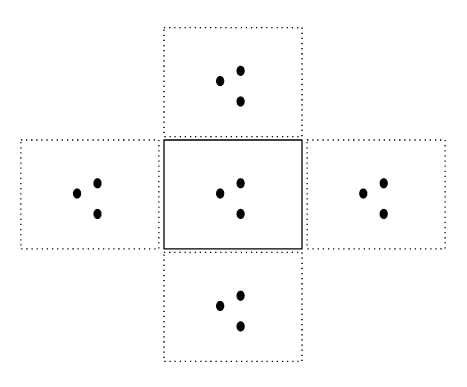
\includegraphics[width=0.7\textwidth]{Figures/pbc}
	\caption{Representation of the periodic boundary condition.}
	\label{fig:pbc}
\end{figure}
\DIFdelbegin %DIFDELCMD < 

%DIFDELCMD < %%%
\DIFdelend \DIFaddbegin \FloatBarrier
\DIFaddend The application of the PBC results in particles interacting not only with each other but also with their images. This fact significantly increases the number of interacting pairs and, consequently, the computational time. To overcome that, we need to choose a limited range potential using the minimum image convention criterion. This criterion only allows a particle to interact with the nearest particle or image.  This is technically done during the simulations by neglecting the interactions between two particles at or beyond a maximum length, which is given the name of cutoff radius ($R_{c}$). This cutoff should be equal to or less than half of the box length. This process of examining each pair separation can also be expensive depending on the number of distinct pairs. That is the reason molecular dynamics algorithms use pair listings. This method defines a 'skin' around the cutoff radius with a radius $R_{List}$, as represented in Figure \ref{fig:pairlist}. The pair list is initially built of all the neighbor particles within a distance $R_{List}$ of each particle. Over the course of the simulation, only pairs in the pair list interact. We then will have a list of all particles j with which a particle i interacts as an example. The pair list must then be updated from time to time during the simulation since particles typically diffuse \cite{tuckerman}.    

\begin{figure}[h]
	\centering
	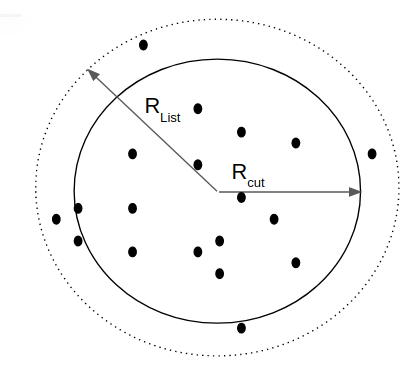
\includegraphics[width=0.5\textwidth]{Figures/pairlist}
	\caption{Representation of the cutoff radius and the pair list radius. Adapted from \citeonline{tuckerman}.}
	\label{fig:pairlist}
\end{figure}
\DIFdelbegin %DIFDELCMD < 

%DIFDELCMD < %%%
\DIFdelend \DIFaddbegin \FloatBarrier
\DIFaddend \subsection{Force Fields }
As said previously, we need to calculate the derivative of the potential energy function in relation to the coordinates in order to update the positions during a simulation. Therefore, we need a model for this potential energy functions. These models are called force fields. They can describe structural characteristics such as van der Waals interactions, bond lengths, bond angles, and torsion in a molecular simulation. The description is done by approximating the potential energy function [$U(r^N)$], which has contributions due to intermolecular and intramolecular interactions. The intramolecular interactions include bond stretching, angle bending, and bond torsion. An illustration of these interactions can be seen in Figure \ref{fig:intraint}. 

\begin{figure}[H]
	\centering
	[a]{{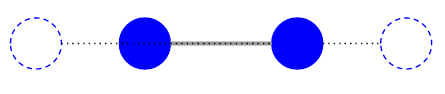
\includegraphics[width=.3\textwidth]{Figures/bondstrech} }}%
	\qquad
	[b]{{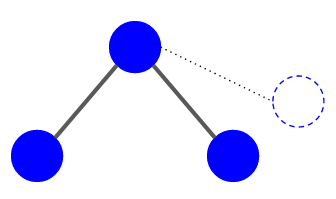
\includegraphics[width=.3\textwidth]{Figures/anglebend} }}%
	\qquad
	[c]{{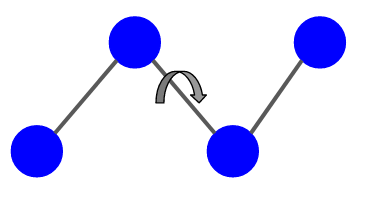
\includegraphics[width=.3\textwidth]{Figures/torsion} }}%    
	\caption{Representation of bond stretching [a], angle bending [b], and bond torsion [c].}%
	\label{fig:intraint}%
\end{figure}


\DIFdelbegin \DIFdel{At }\DIFdelend \DIFaddbegin \DIFadd{In }\DIFaddend this dissertation, we are going to present the equations which are most used to represent these interactions. The contribution to the bond stretching (bs ) is usually given by the harmonic approximation around the energy minimum:

\begin{equation}
u_{bs}(d) = k_{bs} (d - d_{0})^2 .
\end{equation}

Here, $d$ is the bond length, $d_{0}$ is the equilibrium bond length, and $k_{bs}$ is a bond stretching constant. The angle bending (ab) contribution corresponds to deviations from the preferred geometry and is often given by:

\begin{equation}
u_{ab}(\theta) = k_{ab} (\theta - \theta _{0})^2,
\end{equation}
where $k_{ab}$ and $\theta _{0}$ are constants defined by the force field and $\theta$ is the bond angle between three atoms.  The bond torsion (bt) interactions correspond to the energies of rotations around bonds, and it happens among four atoms. A commonly used model is

\begin{equation}
u_{bt}(\omega) = \sum_{n=0}^{N}  c_{n} cos^{n} (\omega) ,
\end{equation}
where N is the number of terms, $c_{n}$ is the coefficient defined by the force field, and $\omega$ is the torsional angle also defined by the force field. 

The other type of interactions, the intermolecular interactions or non-bonded interactions, \DIFdelbegin \DIFdel{include electrostatic }\DIFdelend \DIFaddbegin \DIFadd{can include interactions due to charges, point-dipole moment, }\DIFaddend and van der Waals interactions. The first one represents the interaction between two atoms i and j with partial charges ($q_{i}$ and $q_{j}$) and they are usually represented by Coulomb's Law:

\begin{equation}
u\DIFdelbegin \DIFdel{_{q}}\DIFdelend \DIFaddbegin \DIFadd{_{qq}}\DIFaddend (r_{ij}) = \frac{q_{i}q_{j}}{4 \pi \epsilon _{0} r_{ij}} .
\end{equation} 

In the equation above, $\epsilon _{0}$ is the free space permittivity constant and $r_{ij}$ is the distance between atoms i and j. \DIFaddbegin \DIFadd{The interaction between the partial charges and the dipole moments of particles ($u_{qp}$) and the dipole-dipole ($u_{pp}$) interactions can be expressed as:  
}

\begin{equation}
\DIFadd{u_{qp}(r_{ij}) = \frac{q}{r_{ij}^{3}}(p\bullet \vec{r}_{ij}).
}\end{equation} 

\begin{equation}
\DIFadd{u_{pp}(r_{ij}) = \frac{1}{r_{ij}^{3}}(\vec{p}_{i} \bullet \vec{p}_{j})-\frac{3}{r_{ij}^{5}}(\vec{p}_{i} \bullet \vec{r}_{ij})(\vec{p}_{j} \bullet \vec{r}_{ij}).
}\end{equation} 
\DIFadd{where $p_i$ and $p_j$ are dipole moments of the two particles.
}

\DIFaddend In many force fields, the van der Waals interaction between particles i and j is modeled by the Lennard-Jones Potential:
\begin{equation}
u_{LJ}(r_{ij}) = 4 \epsilon
\left[ \left(\frac{\sigma}{r_{ij}} \right)^{12} - \left(\frac{\sigma}{r_{ij}} \right)^{6} \right],
\end{equation}
where  $\epsilon$ is the depth of the potential well, $\sigma$ is the distance corresponding to a zero intermolecular potential. The graphical representation of the Lennard-Jones potential is presented in Figure \ref{fig:lj}.
\begin{figure}[H]
	\centering
	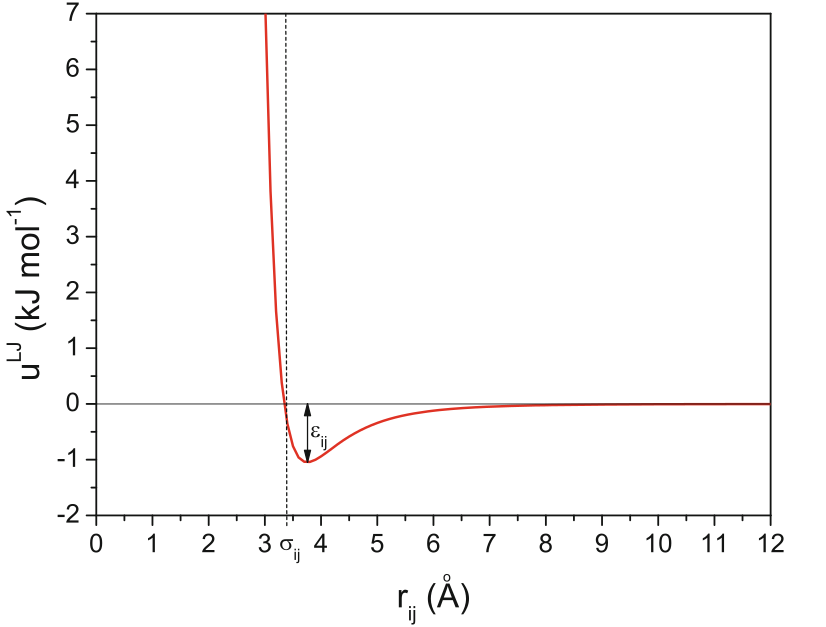
\includegraphics[width=0.8\linewidth]{Figures/lj2}
	\caption{Lennard-Jones potential representation for $\sigma = 1$ and $\epsilon = 1$. }
	\label{fig:lj}
\end{figure}

The potential in Figure \ref{fig:lj} tends to zero and becomes negligible after a specific \DIFaddbegin \DIFadd{large }\DIFaddend value of r. \DIFdelbegin \DIFdel{Hence, we need to set a cutoff radius in which the potential energy is considered to be zero after it}\DIFdelend \DIFaddbegin \DIFadd{In practice, this potential is truncated beyond a certain cutoff}\DIFaddend . The point in which the cutoff is defined is generally the one in which the radial distribution function [$g(r)$] is approximately constant. Also, only interactions with the nearest periodic image of the cell are considered for short-range interactions as explained in \DIFdelbegin \DIFdel{the }\DIFdelend Section \ref{icbc}. With this conditions, the calculations of forces and velocities are computationally feasible. The final potential energy function defined by the force field is then expressed by summing all the interactions above:

\begin{equation}
\DIFdelbegin %DIFDELCMD < \begin{aligned}
%DIFDELCMD < U(r^N) = u_{bs}(d) + u_{ab}(\theta) + u_{bt}(\omega) + u_{q}(r_{ij}) + u_{LJ}(r_{ij}) .
%DIFDELCMD < \end{aligned}
%DIFDELCMD < %%%
\DIFdelend \DIFaddbegin \begin{aligned}
U(r^N) = u_{bs}(d) + u_{ab}(\theta) + u_{bt}(\omega) + u_{qq}(r_{ij}) + u_{qp}(r_{ij})+ u_{pp}(r_{ij})+ u_{LJ}(r_{ij}) .
\end{aligned}
\DIFaddend \end{equation}
%\subsection{title}
%It is possible to impose movements restrictions on the molecule or even consider the molecule as a rigid body in order to increase the integration step or to follow the modeling of the molecules. Methods for this include the SHAKE, RATTLE and Kamberaj algorithms \cite{RYCKAERT1977327,anderson1983,kamberaj}.

\section{SAFT-$\gamma$ Mie Force Field}


\subsection{SAFT-VR Mie Equation of State (EoS)}

The SAFT-VR Mie equation of state \cite{lafitte2013} is the basis for the SAFT-$\gamma$ Mie coarse-grained force field \cite{avendano2011}, which was the force field used to model the molecules used in the simulations carried out in this dissertation. This EoS was initially developed by \citeonline{lafitte2013} to describe chain molecules formed from fused segments interacting via the Mie attractive and repulsive potential. The Mie potential is a type of generalized Lennard-Jones potential that can be used to explicitly describe repulsive interactions of different hardness/softness and attractive interactions of different ranges, and is given by
\begin{equation}
U_{Mie}(r) = \epsilon\frac{\lambda_r}{\lambda_r - \lambda_a} \left(\frac{\lambda_r}{\lambda_a} \right)^{\left( \frac{\lambda_a}{\lambda_r - \lambda_a} \right)}
\left[ \left(\frac{\sigma}{r} \right)^{\lambda_r} - \left(\frac{\sigma}{r} \right)^{\lambda_a} \right],
\label{eqn:miepotential}
\end{equation}
where $\lambda_r$ is the repulsive exponent and $\lambda_a$ is the attractive exponent. The SAFT-VR Mie equation uses the \citeonline{bh1976} high perturbation expansion of the Helmholtz free energy up to the third order and an improved expression for the  radial distribution function (RDF) of Mie monomers at contact to obtain an equation able to give an accurate theoretical description of the vapor-liquid equilibrium and second derivative properties \cite{lafitte2013}. For a non-associating fluid, the Helmholtz free energy is
\begin{equation}
\DIFdelbegin \DIFdel{\frac{A}{N\kappa_{b}T} }\DIFdelend \DIFaddbegin \DIFadd{\frac{A^{SAFT}}{N\kappa_{b}T} }\DIFaddend = a\DIFaddbegin \DIFadd{^{SAFT} }\DIFaddend = a^{IDEAL} + a^{MONO} + a^{CHAIN}, 
\label{eqn:miehelm}
\end{equation}
or, depending on the molecule type, the free energy can be equal to
\begin{equation}
\DIFdelbegin \DIFdel{\frac{A}{N\kappa_{b}T} }\DIFdelend \DIFaddbegin \DIFadd{\frac{A^{SAFT}}{N\kappa_{b}T} }\DIFaddend = a\DIFaddbegin \DIFadd{^{SAFT} }\DIFaddend = a^{IDEAL} + a^{MONO} + a^{RING}.
\label{eqn:miehelmring}
\end{equation}

Here, $a^{IDEAL}$ is the ideal contribution for a mixture. It is given by
\begin{equation}
a^{IDEAL} = \sum_{i=1}^{N_{c}} x_{i}\ln{(\rho_{i}{\Lambda_{i}}^3)} -1 ,
\label{eqn:aideal}
\end{equation}
where \DIFdelbegin \DIFdel{$x_{i}=N_{i}/N$ }\DIFdelend \DIFaddbegin \DIFadd{$x_{i}=N_{i}/N_{c}$ }\DIFaddend is the molar fraction of component i, $N_{i}$ is the number of molecules of each component, \DIFaddbegin \DIFadd{$N_{c}$ is the total number of molecules of the system, }\DIFaddend $\rho_{i}=N_{i}/V$ is the number density, and $\Lambda_{i}^3$ is the de Broglie thermal wavelength. Also in Eq. \ref{eqn:miehelm}, $a^{MONO}$ is the monomer contribution, which  describes interactions between Mie segments and can be expressed, for a mixture, as
\begin{equation}
a^{MONO} = \left(\sum_{i=1}^{N_{c}} x_{i}m_{s,i} \right)a^{M} .
\label{eqn:amonomer}
\end{equation}

In the equation above, $m_{s,i}$ is the number of spherical segments making up the molecule i and $a^{M}$  is the monomer dimensionless Helmholtz free energy. $a^{M}$ is expressed as a third-order perturbation expansion in the inverse temperature \cite{bh1976}:
\begin{equation}
a^{M} = a^{HS}+\beta{a_{1}}+\DIFdelbegin \DIFdel{\beta{a_{2}}^2}\DIFdelend \DIFaddbegin \DIFadd{\beta^{2}{a_{2}}}\DIFaddend +\DIFdelbegin \DIFdel{\beta{a_{3}}^3 }\DIFdelend \DIFaddbegin \DIFadd{\beta^{3} }{\DIFadd{a_{3}}} \DIFaddend . 
\label{eqn:aM}
\end{equation}

Here, $a^{HS}$ is the hard-sphere dimensionless Helmholtz free energy for a mixture and is given by:
\begin{equation}
a^{HS} = \frac{6}{\pi\rho_{s}}\left[\left(\frac{\zeta^3_2}{\zeta^2_3}-\zeta_0 \right)\ln(1-\zeta_3)+\frac{3\zeta_{1}\zeta_{2}}{1-\zeta_3}+ \frac{\zeta^3_2}{\zeta_{3}(1-\zeta_3)^2}\right] .
\label{eqn:hs}
\end{equation}

The variable $\rho_{s}=\rho\sum_{i}^{N_c} x_{i}m_{s,i}$ is the total number density of spherical segments and $\zeta_l$ are the moments of the number density:
\begin{equation}
\zeta_l = \frac{\pi\rho_s}{6}\left(\sum_{i=1}^{N_c} x_{s,i}d_{ii} \right), \quad l = 0,1,2,3 ,
\label{eqn:zetal}
\end{equation}
where $x_{s,i}$ is the mole fraction of segments. It is related to the mole fractions of all component ($x_i$) by:
\begin{equation}
x_{s,i} = \frac{m_{s,i}x_i}{\sum_{k=1}^{N_c} m_{s,k}x_{k} } .
\label{eqn:xsi}
\end{equation}


The effective hard-sphere diameter $d_{ii}$ for the segments is
\begin{equation}
d_{ii} =\int_{0}^{\sigma_{ii}} \left \lbrace 1 - \exp \left [-\beta U^{Mie}_{ii}(r) \right ] \right \rbrace dr .
\label{eqn:diameter}
\end{equation}


The integral in Eq. \eqref{eqn:diameter} is normally obtained by means of a 5-point Gauss-Legendre quadrature \cite{papa2014}. For brevity, the detailing of the other terms of Eq. \eqref{eqn:aM} are available \DIFdelbegin \DIFdel{at }\DIFdelend \DIFaddbegin \DIFadd{in }\DIFaddend the Appendix \ref{restodaseq}. The term $a^{CHAIN}$ in Eq. \ref{eqn:miehelm} corresponds to the chain contribution. This chain formation of $m_{s}$ tangentially bonded Mie segments is based on the first-order perturbation theory (TPT1)  \cite{papa2014} and can be expressed as
\begin{equation}
a^{CHAIN} =-\sum_{i=1}^{N_{c}} x_{i}(m_{s,i} - 1)\ln \left [ g_{ii}^{Mie}(\sigma_{ii}) \right] .
\label{eqn:achain}
\end{equation}

The term $g_{ij}^{Mie}(\sigma_{ij})$ correspond to the radial distribution function (RDF) of the hypothetical Mie system evaluated at the effective diameter. It is obtained with the following perturbation expansion
\begin{equation}
\begin{aligned}
g_{ij}^{Mie}(\sigma_{ij}) =g_{d,ij}^{HS}(\sigma_{ij})\exp \left [\beta\epsilon \frac{g_{1,ij}(\sigma_{ij})}{g_{d,ij}^{HS}(\sigma_{ij})} + (\beta\epsilon)^{2} \frac{g_{2,ij}(\sigma_{ij})}{g_{d,ij}^{HS}(\sigma_{ij})} \right] .
\end{aligned}
\label{eqn:gmie}
\end{equation}


In the equation above, $g_{d,ij}^{HS}$ is equal to 

\begin{equation}
\begin{aligned}
g_{d,ij}^{HS}(\sigma_{ij}) = \exp (k_{0} + k_{1} x_{0,ij} + k_{2} x_{0,ij}^{2} + k_{3} x_{0,ij}^{3}) ,
\end{aligned}
\label{eqn:ghs}
\end{equation}
where $x_{0,ij} = \sigma_{ij}/d_{ij}$ and $k_{1}, k_{2},$ and $k_{3}$ are density dependent coefficients. These coefficients and the other terms of Eq. \ref{eqn:gmie} are available \DIFdelbegin \DIFdel{at }\DIFdelend \DIFaddbegin \DIFadd{in }\DIFaddend Appendix \ref{restodaseq}.  

The ring contribution ($a^{RING}$) in Eq. \ref{eqn:miehelmring} have two forms for rings formed from tangentially bonded segments. The first was developed by \citeonline{lafitte2012}. It considers that the difference between a chain and a ring molecule is that the latter has one more bond that is connecting the first segment to the last. With this assumption, Eq.~\eqref{eqn:achain} can be adapted to rings by
\begin{equation}
a^{RING} =-\sum_{i=1}^{N_{c}} x_{i}m_{s,i}\ln[g_{ii}^{Mie}(\sigma_{ii})] .
\label{eqn:aringlafitte}
\end{equation}

According to \citeonline{lafitte2012}, Eq. \eqref{eqn:aringlafitte} needs an additional parameterization with molecular simulation data so that the EoS can  be used in molecular simulations, but this additional parameterization is not necessary when we are modeling chain molecules. Recently, \citeonline{muller2017} tried to correct this inconsistency. They developed a Helmholtz free energy equation for rings based on the work of \citeonline{muller1993}, who obtained rigorous expressions for hard-sphere fluids with molecular geometries of rings with $m_s=3$. The final expression developed for the dimensionless Helmholtz free energy due to ring formation is
\begin{equation}
a^{RING} =-\sum_{i=1}^{N_{c}} x_{i}\left (m_{s,i}-1+\chi_{i}\eta_{i} \right )\ln \left [g_{ii}^{Mie}(\sigma_{ii}) \right] ,
\label{eqn:aringmuller}
\end{equation}
where $\eta_{i}=m_{s,i}\rho_{i}\sigma_{ii}^{3}/6$ is the packing fraction of the atom i and $\chi_{i}$ is a parameter which depends on $m_{s,i}$ and \DIFdelbegin \DIFdel{on }\DIFdelend the geometry of the ring of each component i. For a value of $\chi=0$, Eq. \eqref{eqn:aringmuller} is equal to Eq. \eqref{eqn:achain}. In addition, the equation corresponds to a system of hard sphere triangles when $\chi=1.3827$. \citeonline{muller2017} also calculated values of $\chi$ for $m_{s}=3,m_{s}=4,m_{s}=5$, and $m_{s}=7$ \DIFdelbegin \DIFdel{with }\DIFdelend \DIFaddbegin \DIFadd{using a geometry formed by a system of equilateral triangles. In these calculations, they used }\DIFaddend pseudo-experimental data from molecular dynamics (MD) for a defined pure fluid with $\epsilon/\kappa_{b} = 250 K$, $\sigma = 3.0 \dot{A}$, $\lambda_{r} = 11$, and $\lambda_{r} = 6$. Values of $\chi$  for some of the geometry estimated in their article can be seen in \figref{ringqsi}.
\DIFaddbegin 

\DIFaddend \begin{figure}[th]
	\centering
	\DIFdelbeginFL %DIFDELCMD < 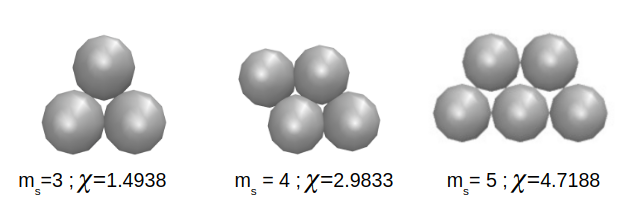
\includegraphics[scale=0.5]{Figures/mullergeo.png}
%DIFDELCMD < 	%%%
\DIFdelendFL \DIFaddbeginFL 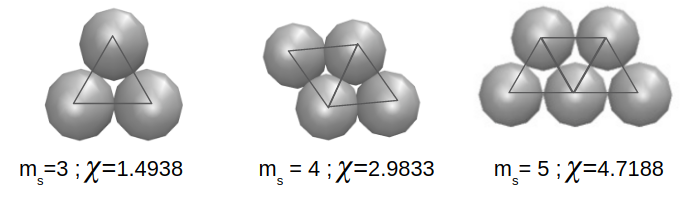
\includegraphics[scale=0.5]{Figures/mullercomtrian}
	\DIFaddendFL \caption{Values for parameter $\chi$ according to the ring geometry. Adapted from \citeonline{muller2017}.}
	\label{ringqsi}
\end{figure}

\citeonline{lafitte2013} also suggested mixing rules for this EoS parameters based on Lorentz-Berthelot combining rules \cite{rowlinson}:
\begin{equation}
\sigma_{ij} =\frac{\sigma_{ii}+\sigma_{jj}}{2},
\label{eqn:sigmamix}
\end{equation}
\begin{equation}
d_{ij} =\frac{d_{ii}+d_{jj}}{2},
\label{eqn:dmix}
\end{equation}
\begin{equation}
\lambda_{k,ij} -3 =\sqrt{(\lambda_{k,ii}-3)(\lambda_{k,jj}-3)},  \quad k=r,a,
\label{eqn:lambdamix}
\end{equation}
\begin{equation}
\epsilon_{ij} =(1-k_{ij})\frac{\sqrt{\sigma_{ii}^{3}\sigma_{jj}^{3}}}{\sigma_{ij}^{3}}\sqrt{\epsilon_{ii}\epsilon_{jj}}.
\label{eqn:epsmix}
\end{equation}

The $k_{ij}$ is a binary interaction parameter to correct the deviations of the mixing rule\DIFdelbegin \DIFdel{for chemically distinct compounds that can be fitted to experimental or molecular simulation data. This necessity of an additional parameter raises the question of the quality of these mixing rules and make us wonder if new mixing rules could be used to describe the mixing potential well parameter. Since these were the available mixing rules and the ones }\DIFdelend \DIFaddbegin \DIFadd{. This parameter can be described as scaling factor. It is necessary to account the interactions among chemically distinct compounds, which are not explicitly considered by the SAFT-VR Mie EoS. These mixing rules were the ones available in the literature and }\DIFaddend employed by other papers that used this force field\DIFaddbegin \DIFadd{. Therefore}\DIFaddend , we ended up using Eqs. \ref{eqn:sigmamix} to \ref{eqn:epsmix} in our study. However, the binary interaction parameter was only necessary for aqueous mixtures in our study.  \DIFaddbegin \DIFadd{Having the dimensionless Helmholtz free energy exposed in the equations above, we can now calculate the derivative properties with the fundamental thermodynamic equation (Eq. \ref{eq:fteq}) using the EoS. The output from these calculations are then used to estimate the parameters of the SAFT-$\gamma$ Mie force field. 
}\DIFaddend 


\subsection{Parameter Estimation for the SAFT-$\gamma$ Mie Force Field}\label{parsaft}

The SAFT-$\gamma$ Mie Force Field uses a top-down coarse-graining methodology in its parameterization. This methodology aims to obtain the intermolecular parameters from macroscopic experimental data such as fluid-phase equilibrium or interfacial tension data. The idea is that the force field parameters estimated with the SAFT-VR Mie EoS can be used in molecular simulations since both the equation of state and the force field use the same explicit intermolecular potential model (Mie potential). This correspondence between models has been used to parametrize a variety of fluids \cite{ervik2016}. This force field has the advantage of incorporating the degrees of freedom provided by the use of the Mie Potential \cite{herdes2015}. This flexibility offers the exploration of a vast parameter space without using an iterative simulation scheme \cite{avendano2011}. Despite these advantages, the force field can be restricted by the shortcomings of the equation of state. As an example, the lack of an association term in the equation can cause an inadequate representation of the properties of hydrogen bonding compounds.

Each substance has initially five parameters to be estimated ($m_s,\ \sigma,\ \epsilon,\ \lambda_{r},$ and $, \lambda_{a}$) according to Eq. \eqref{eqn:miepotential}. The number of segments is usually fixed in an integer value since each segment represents one pseudo atom. The attractive parameter is generally  fixed due to its  high correlation with the repulsive parameter. Usually, the chosen value for this parameter is 6, corresponding to the London model, which is a good representation of the dispersion scale of most simple fluids that do not have strong polar interactions \cite{ramrattan2015,herdes2015}. There are two strategies to obtain the parameters: one is by fitting the SAFT-VR Mie EoS to experimental data such as vapor pressure, liquid density and the other one is by using corresponding states parametrization. The first was the one followed in this dissertation. Generally, this approach minimizes the following unweighted least-squares objective function:

\begin{equation}
\DIFdelbegin %DIFDELCMD < \begin{aligned}
%DIFDELCMD < \min\limits_{\sigma,\epsilon,\lambda_{r}} F_{obj}= \sum_{i=1}^{N_{p}} \left[\frac{P_{v}^{SAFT}(T_{i},\sigma,\epsilon,\lambda_{r})-P_{v}^{exp}(T_{i})}{P_{v}^{exp}(T_{i})} \right]^2 +\\
%DIFDELCMD < \sum_{i=1}^{N_{p}} \left[\frac{\rho_{l}^{SAFT}(T_{i},\sigma,\epsilon,\lambda_{r})-\rho_{l}^{exp}(T_{i})}{\rho_{l}^{exp}(T_{i})} \right]^2 ,
%DIFDELCMD < \end{aligned}
%DIFDELCMD < %%%
\DIFdelend \DIFaddbegin \begin{aligned}
F_{obj}= \sum_{i=1}^{N_{p}} \left[\frac{P_{v}^{SAFT}(T_{i},\sigma,\epsilon,\lambda_{r})-P_{v}^{exp}(T_{i})}{P_{v}^{exp}(T_{i})} \right]^2 +\\
\sum_{i=1}^{N_{p}} \left[\frac{\rho_{l}^{SAFT}(T_{i},\sigma,\epsilon,\lambda_{r})-\rho_{l}^{exp}(T_{i})}{\rho_{l}^{exp}(T_{i})} \right]^2 ,
\end{aligned}
\DIFaddend \label{eqn:fobj}
\end{equation}
where $N_{p}$ is the number of experimental points, $P_{v}$ is the vapor pressure, and $\rho_{l}$ is the saturated liquid density. Other properties that can be used in the estimation are interfacial tension and speed of sound, for instance. The multiple parameters of the model make it necessary the use of a wide range of experimental data since multiple solutions may be found for the fit. Therefore, one needs to be careful in deciding the level of coarse-graining (i.e. the choice of parameter $m_{s}$) and the subsequent parameter space so as to avoid some physical inconsistencies such as a premature freezing \cite{lobanova2015}.

\citeonline{lafitte2012} suggested that two correction factors ($c_{\sigma}$ and $c_{\epsilon}$) should be estimated with simulation data when using Eq. \eqref{eqn:aringlafitte} for the ring contribution. They are related to the EoS parameters by scaled parameters:

\begin{equation}
\sigma^{scaled} = c_{\sigma}\sigma^{SAFT}.
\label{eqn:csigma}
\end{equation}
\begin{equation}
\epsilon^{scaled} = c_{\epsilon}\epsilon^{SAFT}.
\label{eqn:ceps}
\end{equation}

According to \citeonline{lafitte2012}, these corrections are necessary because the approximations employed in the EoS theory generate discrepancies between molecular simulations and the EoS for ring molecules modeled with Eq. \eqref{eqn:aringlafitte}. However, this new parameterization is not necessary when using Eq. \eqref{eqn:aringmuller} as the ring contribution or when we are modeling chain molecules with Eq. \ref{eqn:achain}. This fact makes the strategy of \citeonline{lafitte2012} inconsistent since parameterization with molecular simulation should not be necessary according to the overall idea of this force field. Furthermore, the use of molecular simulation data highly increases the time spent on the parameterization process. The objective function for the estimation of the correction parameter is given by

\begin{equation}
\DIFdelbegin %DIFDELCMD < \begin{split}
%DIFDELCMD < \min\limits_{c_{\sigma},c_{\epsilon}} F_{obj}= \sum_{i=1}^{N_{p}} \left[\frac{P_{v}^{sim}(T_{i},\sigma^{SAFT},\epsilon^{SAFT})-P_{v}^{SAFT}(T_{i},\sigma^{scaled},\epsilon^{scaled})}{P_{v}^{sim}(T_{i},\sigma^{SAFT},\epsilon^{SAFT})} \right]^2 + \\
%DIFDELCMD < \sum_{i=1}^{N_{p}} \left[\frac{\rho_{liq}^{sim}(T_{i},\sigma^{SAFT},\epsilon^{SAFT})-\rho_{liq}^{SAFT}(T_{i},\sigma^{scaled},\epsilon^{scaled})}{\rho_{liq}^{sim}(T_{i},\sigma^{SAFT},\epsilon^{SAFT})} \right]^2 .
%DIFDELCMD < \end{split}
%DIFDELCMD < %%%
\DIFdelend \DIFaddbegin \begin{split}
F_{obj}= \sum_{i=1}^{N_{p}} \left[\frac{P_{v}^{sim}(T_{i},\sigma^{SAFT},\epsilon^{SAFT})-P_{v}^{SAFT}(T_{i},\sigma^{scaled},\epsilon^{scaled})}{P_{v}^{sim}(T_{i},\sigma^{SAFT},\epsilon^{SAFT})} \right]^2 + \\
\sum_{i=1}^{N_{p}} \left[\frac{\rho_{liq}^{sim}(T_{i},\sigma^{SAFT},\epsilon^{SAFT})-\rho_{liq}^{SAFT}(T_{i},\sigma^{scaled},\epsilon^{scaled})}{\rho_{liq}^{sim}(T_{i},\sigma^{SAFT},\epsilon^{SAFT})} \right]^2 .
\end{split}
\DIFaddend \label{eqn:fobjla}
\end{equation}

The repulsive parameter is maintained in the value found on the minimization of Eq. \eqref{eqn:fobj}. The refined values for $\sigma$ and $\epsilon$ are

\begin{equation}
\sigma^{sim} = \sigma^{SAFT}/c_{\sigma},
\label{eqn:simsigma}
\end{equation}

\begin{equation}
\epsilon^{sim} = \epsilon^{SAFT}/c_{\epsilon},
\label{eqn:simeps}
\end{equation}

The other method to obtain the force field parameters is the corresponding states parametrization \cite{mejia2014}. This method considers that the unweighted volume average of the attractive contribution to the Mie intermolecular potential, $ \, a_{1}$, is the following mean-field approximation

\begin{equation}
a_{1} = 2\pi\rho\sigma^{3}\epsilon\alpha .
\label{eqn:a1corres}
\end{equation}

The van der Waals constant, $\alpha$, considering $ \lambda_{a} = 6$ is related by the Mie exponents by

\begin{equation}
\alpha = \frac{1}{\epsilon\sigma^{3    }} \int_{\sigma}^{\infty} \phi(r)r^{2}dr = \frac{\lambda_{r}}{3(\lambda_{r}-3)}\left(\frac{\lambda_r}{6}\right)^{6/(\lambda_{r} - 6)}  .
\label{eqn:alpha}
\end{equation}

The parameterization in this method starts by using the experimental acentric factor, $\omega$, for each molecule with a fixed value of $ m_{s}$ \DIFaddbegin \DIFadd{in order }\DIFaddend to obtain the value of the repulsive exponent with the following Padé series:

\begin{equation}
\lambda_{r} = \frac{\sum_{i=0} a_{i}\omega^{i}}{1+\sum_{i=1} b_{i}\omega^{i}} ,  
\label{eqn:lambdaco}
\end{equation}
where $a_{i}$ and $b_{i}$ are parameters that are dependent on the number of segments. A table with these parameters is presented in the original paper \cite{mejia2014}. The van der Waals constant can be found by substituting $\lambda_{r}$ into Eq. \eqref{eqn:alpha}. The reduced critical temperature $T_{c}^{*}$ is related to $\alpha$ by a Padé series: 

\begin{equation}
T_{c}^{*} = \frac{\sum_{i=0} c_{i}\alpha^{i}}{1+\sum_{i=1} d_{i}\alpha^{i}}   .
\label{eqn:tc}
\end{equation}

The values of $c_{i}$ and $d_{i}$ are also available in the original paper. The reduced temperature of the equation above is used in conjunction with the experimental critical temperature, $ T_{c}$, to find the energy parameter with the relation below:

\begin{equation}
T_{c}^{*} = \frac{\kappa_{b}T_{c}}{\epsilon}   .
\label{eqn:epscorre}
\end{equation}

The diameter parameter, however, is not obtained with the critical properties, but with the reduced liquid density at the reduced temperature of $0.7$ ($\rho_{T_{r}=0.7}$). This density is also obtained with a Padé series using parameters by \citeonline{mejia2014}:

\begin{equation}
\rho_{T_{r}=0.7}^{*} = \DIFdelbegin \DIFdel{\frac{\sum_{i=0} j_{i}\alpha^{i}}{1+\sum_{i=1} k_{i}\alpha^{i}} }\DIFdelend \DIFaddbegin \DIFadd{\frac{\sum_{i=0} e_{i}\alpha^{i}}{1+\sum_{i=1} f_{i}\alpha^{i}} }\DIFaddend .
\label{eqn:denscorre}
\end{equation}

The \DIFaddbegin \DIFadd{coefficients $a_{i}, b_{i}, ...,f_{i}$ depend on the number of segments, and they are available in the literature for ring and chain geometries \mbox{%DIFAUXCMD
\cite{muller2017,mejia2014}}%DIFAUXCMD
. The }\DIFaddend relation between the \DIFdelbegin \DIFdel{equation above}\DIFdelend \DIFaddbegin \DIFadd{Eq. \ref{eqn:denscorre}}\DIFaddend , $\sigma$ and the experimental density is given by

\begin{equation}
\rho_{T_{r}=0.7}^{*} = \rho_{T_{r}=0.7}\sigma^{3}N_{av},   
\label{eqn:sigmacorre}
\end{equation}
where $N_{av}$ is the Avogadro number. This corresponding states method has the advantage of only requiring critical data, which is available for a great range of fluids, and liquid density data. The parameters \DIFdelbegin \DIFdel{found with this strategy }\DIFdelend \DIFaddbegin \DIFadd{obtained with these parameterization strategies }\DIFaddend are available at \DIFdelbegin \DIFdel{an online database \mbox{%DIFAUXCMD
\cite{ervik2016}}%DIFAUXCMD
.     
}%DIFDELCMD < 

%DIFDELCMD < %%%
\DIFdel{The }\DIFdelend \DIFaddbegin \DIFadd{a large online database for this force field \mbox{%DIFAUXCMD
\cite{ervik2016}}%DIFAUXCMD
. Here, we only expose the coarse-grained geometries and the sets of parameters for the compounds used in this dissertation. They are available  at Tables  \ref{tbl:parameters} and \ref{tbl:geopara}. The parameters for water were retrieved from \mbox{%DIFAUXCMD
\citeonline{lobanova2016}}%DIFAUXCMD
; for carbon dioxide, propane, and hexane from \mbox{%DIFAUXCMD
\citeonline{herdes2015}}%DIFAUXCMD
; for 1-octanol from \mbox{%DIFAUXCMD
\citeonline{ervik2016}}%DIFAUXCMD
; and for the aromatic compounds from   \mbox{%DIFAUXCMD
\citeonline{muller2017}}%DIFAUXCMD
.     
}

\begin{table}[h]
	\centering
	\caption{\DIFaddFL{Parameters of the SAFT-$\gamma$ Mie force field for each substance used in this work.}}
	\label{tbl:parameters}
	\begin{tabular}{ccccc}
		\hline
		\hline
		& \DIFaddFL{$m_s$ }& \DIFaddFL{$\epsilon/\kappa_{b}$ (K) }& \DIFaddFL{$\sigma$ (\AA) }& \DIFaddFL{$\lambda_r$ }\\ \hline\hline
		\DIFaddFL{Water          }& \DIFaddFL{1     }& \DIFaddFL{305.21               }& \DIFaddFL{2.902              }& \DIFaddFL{8.0         }\\
		\DIFaddFL{Carbon dioxide }& \DIFaddFL{2     }& \DIFaddFL{194.94               }& \DIFaddFL{2.848              }& \DIFaddFL{14.65       }\\
		\DIFaddFL{Propane        }& \DIFaddFL{1     }& \DIFaddFL{426.08               }& \DIFaddFL{4.871              }& \DIFaddFL{34.29       }\\
		\DIFaddFL{Hexane         }& \DIFaddFL{2     }& \DIFaddFL{376.35               }& \DIFaddFL{4.508              }& \DIFaddFL{19.57       }\\
		\DIFaddFL{1-octanol        }& \DIFaddFL{3     }& \DIFaddFL{495.71               }& \DIFaddFL{4.341              }& \DIFaddFL{28.79       }\\
		\DIFaddFL{Toluene        }& \DIFaddFL{3     }& \DIFaddFL{268.24               }& \DIFaddFL{3.685              }& \DIFaddFL{11.80       }\\
		\DIFaddFL{Benzene        }& \DIFaddFL{3     }& \DIFaddFL{230.30               }& \DIFaddFL{3.441              }& \DIFaddFL{10.45       }\\
		\DIFaddFL{Pyrene         }& \DIFaddFL{4     }& \DIFaddFL{459.04               }& \DIFaddFL{4.134              }& \DIFaddFL{15.79       }\\
		\DIFaddFL{Anthracene     }& \DIFaddFL{5     }& \DIFaddFL{259.68               }& \DIFaddFL{3.631              }& \DIFaddFL{9.55        }\\ 
		\hline
		\hline
	\end{tabular}

\end{table}

\DIFadd{When modeling mixtures with this force field, it can be necessary to estimate the }\DIFaddend binary interaction parameter $k_{ij}$ of Eq. \eqref{eqn:epsmix}\DIFdelbegin \DIFdel{is necessary to adjust the mixture behavior of chemically distinct components. Normally, it is }\DIFdelend \DIFaddbegin \DIFadd{. This parameter is normally }\DIFaddend estimated by minimizing the difference between experimental binary vapor-liquid equilibrium or interfacial tension data and the SAFT-VR Mie EoS output data \cite{muller2017,lobanova2016}. The objective function is similar to: 

\begin{equation}
\DIFdelbegin %DIFDELCMD < \begin{aligned}
%DIFDELCMD < \min\limits_{k_{ij}} F_{obj}= \sum_{k=1}^{N_{p}} \left(\frac{P_{v}^{SAFT}(T_{k},x,k_{ij})-P_{v}^{exp}(T_{k},x)}{P_{v}^{exp}(T_{k},x)} \right)^2 +\\
%DIFDELCMD < \sum_{k=1}^{N_{p}} \left(\frac{\rho_{l}^{SAFT}(T_{k},x,k_{ij})-\rho_{l}^{exp}(T_{i})}{\rho_{l}^{exp}(T_{i})} \right)^2 .
%DIFDELCMD < \end{aligned}
%DIFDELCMD < %%%
\DIFdelend \DIFaddbegin \begin{aligned}
F_{obj}= \sum_{k=1}^{N_{p}} \left(\frac{P_{v}^{SAFT}(T_{k},x,k_{ij})-P_{v}^{exp}(T_{k},x)}{P_{v}^{exp}(T_{k},x)} \right)^2 +\\
\sum_{k=1}^{N_{p}} \left(\frac{\rho_{l}^{SAFT}(T_{k},x,k_{ij})-\rho_{l}^{exp}(T_{i})}{\rho_{l}^{exp}(T_{i})} \right)^2 .
\end{aligned}
\DIFaddend \label{eqn:fobjmix}
\end{equation}

However, \citeonline{ervik20162} used molecular simulation results to fit the parameter to the interfacial tension data. The strategy they followed was to carry out simulations in three values of $k_{ij}$ first and, after, refine the parameter until a value in good agreement with the experimental data is found. We decided to follow this strategy in our estimations of $k_{ij}$ since the estimation with the EoS did not provide satisfactory results for the hydration free energy calculations. 

\DIFaddbegin \begin{table}[h]
	\caption{\DIFaddFL{Coarse-grained geometries of the substances used in this work for the SAFT-$\gamma$ Mie force field.}}
	\centering
	\label{tbl:geopara}
	\begin{tabular}{ccc}

		\toprule \toprule
		\DIFaddFL{Molecule }&  \DIFaddFL{Structure }&  \DIFaddFL{Coarse grained structure  }\\
		\midrule \midrule
		\DIFaddFL{Water }&
		\adjustimage{height=1.2cm,valign=m}{Figures/waterg} &
		\adjustimage{height=1cm,valign=m}{Figures/onebead}  \\
		\DIFaddFL{Carbon dioxide }&
		\adjustimage{height=0.8cm,valign=m}{Figures/co2g} &
		\adjustimage{height=1cm,valign=m}{Figures/twobeads}  \\
		\DIFaddFL{Propane }& \adjustimage{height=1.5cm,valign=m}{Figures/propg}  & \adjustimage{height=1cm,valign=m}{Figures/onebead} \\
		\DIFaddFL{Hexane }& \adjustimage{height=1.5cm,valign=m}{Figures/hexg}  & \adjustimage{height=1cm,valign=m}{Figures/twobeads} \\
		\DIFaddFL{1-octanol }& \adjustimage{height=1.5cm,valign=m}{Figures/octg}  & \adjustimage{height=1cm,valign=m}{Figures/threebeads} \\
		\DIFaddFL{Toluene }& \adjustimage{height=2.5cm,valign=m}{Figures/tolg}  & \adjustimage{height=2cm,valign=m}{Figures/fe3} \\
		\DIFaddFL{Benzene }& \adjustimage{height=2.5cm,valign=m}{Figures/benzg}  & \adjustimage{height=2cm,valign=m}{Figures/fe3} \\
		\DIFaddFL{Pyrene }& \adjustimage{height=2.5cm,valign=m}{Figures/pyre}  & \adjustimage{height=2cm,valign=m}{Figures/pyrecg} \\
		\DIFaddFL{Anthracene }& \adjustimage{height=2cm,valign=m}{Figures/ant}  & \adjustimage{height=2cm,valign=m}{Figures/fen5} \\
		\bottomrule \bottomrule

	\end{tabular}
\end{table}
\FloatBarrier
\DIFaddend \section{Solvation Free Energy Calculations Based on Molecular Dynamics}
% background topics

Using the SAFT-$\gamma$ Mie Force Field described in the section above, we carried out solvation free energy molecular dynamics simulations. The free energies we are trying to calculate can be expressed as averages over ensembles of atomic configurations generated using Monte Carlo or Molecular Dynamics techniques. In the canonical ensemble, the free energy is given by  

\begin{equation}
\label{eq:fcano}
\begin{aligned}
F(N,V,T) = -\kappa_{b}T \ln Q(N,V,T).
\end{aligned}
\end{equation}

Recall that $Q(N,V,T)$ is the partition function of the canonical ensemble, expressed as

\begin{equation}
\label{eq:partican}
\DIFdelbegin %DIFDELCMD < \begin{aligned}
%DIFDELCMD < Q(N,V,T) =\frac{\epsilon_{0}}{h^{3N}N!} \int d^{n}p d^{n}r \exp \left[ -\beta \left( \sum_{i=1}^{N}\dfrac{p_{i}^{2}}{2m_{i}} + U(r_{1},..,r_{n}) \right)
%DIFDELCMD < \right] .
%DIFDELCMD < \end{aligned}
%DIFDELCMD < %%%
\DIFdelend \DIFaddbegin \begin{aligned}
Q(N,V,T) =\frac{1}{h^{3N}N!} \int dp^{n} dr^{n} \exp \left[ -\beta \left( \sum_{i=1}^{N}\dfrac{p_{i}^{2}}{2m_{i}} + U(r_{1},..,r_{n}) \right)
\right] .
\end{aligned}
\DIFaddend \end{equation}

The Gibbs free energy, the object of study in this dissertation, is given by

\begin{equation}
\begin{aligned}
G(N,P,T) = -\kappa_{b}T ln \Delta (N,P,T),
\end{aligned}
\end{equation}
where $\Delta (N,P,T)$ is the partition function of the isothermal-isobaric ensemble:

\begin{equation}
\DIFdelbegin %DIFDELCMD < \begin{aligned}
%DIFDELCMD < \Delta (N,P,T) = \frac{1}{V_{0}} \int_{0}^{\infty} dV \int d^{n}p d^{n}r \exp \left[ -\beta \left( \sum_{i=1}^{N}\dfrac{p_{i}^{2}}{2m_{i}} + U(r_{1},..,r_{n}) + PV(r_{1},..,r_{n}) \right) \right].
%DIFDELCMD < \end{aligned}
%DIFDELCMD < %%%
\DIFdelend \DIFaddbegin \begin{aligned}
\Delta (N,P,T) = \frac{1}{V_{0}N!h^{3N}} \int_{0}^{\infty} dV \int dp^{n} dr^{n} \exp \left[ -\beta \left( \sum_{i=1}^{N}\dfrac{p_{i}^{2}}{2m_{i}} + U(r_{1},..,r_{n}) + PV(r_{1},..,r_{n}) \right) \right].
\end{aligned}
\DIFaddend \end{equation}

Evaluating the partition function is an often unfeasible task, but we are interested in calculating only the Gibbs free energy difference between two states of a system, which is  

\begin{equation}
\begin{aligned}
\Delta G_{AB} = G_{B} - G_{A}= -\kappa_{b}T ln \left( \frac{\Delta_{B}}{\Delta_{A}}\right) .
\end{aligned}
\end{equation}

Since the masses of particles in states A and B of a system are the same and the Hamiltonian is separable in $K(p)$ and $U(r)$, the moment integrals in the ratio ${\Delta_{B}}/{\Delta_{A}}$ can be simplified into the ratio of the configuration integrals:

\begin{equation}
\label{eq:partiso}
\DIFdelbegin %DIFDELCMD < \begin{aligned}
%DIFDELCMD < \dfrac{Z_{B}}{Z_{A}} = \dfrac{\int_{0}^{\infty} dV \int d^{n}r \exp \left\lbrace -\beta \left[U(r_{1},..,r_{n}) + PV(r_{1},..,r_{n}) \right]_{B} \right\rbrace}{\int_{0}^{\infty} dV \int d^{n}r \exp \left\lbrace  -\beta \left[U(r_{1},..,r_{n}) + PV(r_{1},..,r_{n}) \right]_{A} \right\rbrace }.
%DIFDELCMD < \end{aligned}
%DIFDELCMD < %%%
\DIFdelend \DIFaddbegin \begin{aligned}
\dfrac{Z_{B}}{Z_{A}} = \dfrac{\int_{0}^{\infty} dV \int dr^{n} \exp \left\lbrace -\beta \left[U(r_{1},..,r_{n}) + PV(r_{1},..,r_{n}) \right]_{B} \right\rbrace}{\int_{0}^{\infty} dV \int dr^{n} \exp \left\lbrace  -\beta \left[U(r_{1},..,r_{n}) + PV(r_{1},..,r_{n}) \right]_{A} \right\rbrace }.
\end{aligned}
\DIFaddend \end{equation}

This identity results in the following equation for the Gibbs free energy difference, which does not  require the calculation of the partition function at each state:

\begin{equation}
\label{eq:dif}
\begin{aligned}
\Delta G_{AB} = G_{B} - G_{A}= -\kappa_{b}T ln \left( \frac{Z_{B}}{Z_{A}}\right).
\end{aligned}
\end{equation}

In the case of a study concerning the solvation of a single molecule, the Gibbs free energy difference between end states $A$ and $B$ are, more specifically, the difference between the solute alone in the gas phase and the solute interacting with the solvent. In order to have accurate results for free energy differences, the states need to have sufficient overlap  \cite{klimovich}. The overlap can be achieved by calculating the free energy difference among a series of intermediates states. The result of these differences is independent of the path chosen since free energy is a state function. That is why alchemical states (without physical sense) can be used to link physical states of interest. The solvation free energy calculations are then done through a thermodynamic path in which the solute molecule is gradually inserted into the solvent as illustrated in \figref{thermcy}. According to this path, the free energy of solvation is expressed as

\begin{equation}
\label{eq:freesolv}
\begin{aligned}
\Delta G_{solv} = \Delta G_{1 \rightarrow 4} = \Delta G_{1 \rightarrow 2} + \Delta G_{2 \rightarrow 3} + \Delta G_{3 \rightarrow 4}  - \kappa_{b}T \ln \dfrac{V^{*}}{V^{1}} .
\end{aligned}
\end{equation}

\DIFdelbegin %DIFDELCMD < \begin{figure}[th]
%DIFDELCMD < 	\centering
%DIFDELCMD < 	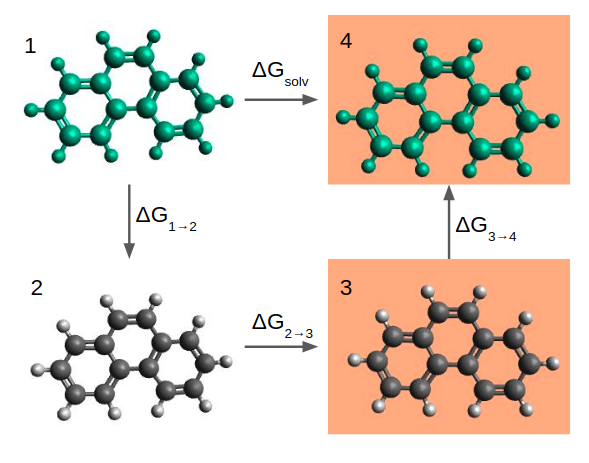
\includegraphics[scale=0.6]{Figures/cicclotermo}
%DIFDELCMD < 	%%%
%DIFDELCMD < \caption{%
{%DIFAUXCMD
\DIFdelFL{Thermodynamic path for computing solvation free energy of a single solute molecule with molecular dynamics. Adapted from \mbox{%DIFAUXCMD
\citeonline{klimovich}}%DIFAUXCMD
.}}
	%DIFAUXCMD
%DIFDELCMD < %DIFDELCMD < \label{thermcy}%%%
%DIFDELCMD < \end{figure}
%DIFDELCMD < 

%DIFDELCMD < %%%
\DIFdelend The last term in Eq. \ref{eq:freesolv} accounts for the difference between the mean volume of the simulation box with the solute inserted ($V_{1}$) and the mean volume of the simulation box with only solvent molecules in it ($V^{*}$). However, \citeonline{shirts2013} have shown that this term is negligible with respect to the statistical uncertainty of calculating $\Delta G$. In addition, when we have other solute molecules \DIFdelbegin \DIFdel{that are equal to the solute molecule being inserted in the box}\DIFdelend \DIFaddbegin \DIFadd{in solution}\DIFaddend , another term in Eq. \ref{eq:freesolv} \DIFdelbegin \DIFdel{can appear in order to distinguish these molecules }\DIFdelend \DIFaddbegin \DIFadd{may be necessary }\DIFaddend \cite{shirts2013}. The term $\Delta G_{1 \rightarrow 2}$, also represented in \figref{thermcy},  is the solvation free energy associated with turning off the non bonded interactions of the molecule in the gas phase. In the next transformation, $\Delta G_{2 \rightarrow 3}$ is the free energy of moving the non-interacting molecule from the gas phase to the solvent and is equal to zero since the transformation of a non-interacting molecule does not depend on the environment. Lastly, $\Delta G_{3 \rightarrow 4}$ is the free energy required for the non-interaction molecule in the solvent phase to regain its non-bonded interactions with the solvent.  The solvation free energy calculation can be classified according to the types of non-bonded interactions that are turned off/on in the $1 \rightarrow 2$ and $ 3 \rightarrow 4$ parts of the path. If both non-bonded interactions with the environment and internal interactions are turned off, this is an annihilation free energy calculation. On the other hand, if only non-bonded interactions with the environment are turned off, this is a decoupling free energy calculation \cite{klimovich}. In the latter case, $\Delta G_{1 \rightarrow 2} = 0$ and the $\Delta G_{solv} = \Delta G_{3 \rightarrow 4} $.  

\DIFaddbegin \begin{figure}[h]
	\centering
	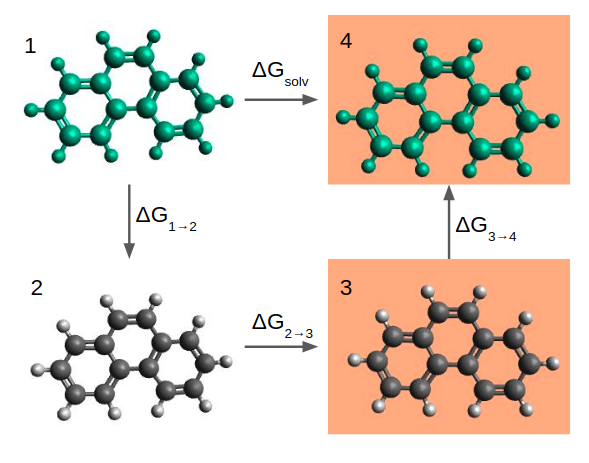
\includegraphics[scale=0.6]{Figures/cicclotermo}
	\caption{\DIFaddFL{Thermodynamic path for computing solvation free energy of a single solute molecule with molecular dynamics. Adapted from \mbox{%DIFAUXCMD
\citeonline{klimovich}}%DIFAUXCMD
.}}
	\label{thermcy}
\end{figure}

\DIFaddend The methods used to carry out the transformations of Figure \ref{thermcy} during the simulation scale the solute charges to zero and then turn off the interactions corresponding to the Lennard-Jones or Mie potential. In order to carry out the latter process, a modified potential with a coupling parameter ($\lambda$) is used. Each $\lambda$ represents an alchemical state. When $\lambda=0$, there is no interaction with the solvent and, when $\lambda=1$, interactions are fully activated. The coupling of the $\lambda$ parameter could be linear, \DIFaddbegin \DIFadd{as it is demonstrated in Figure \ref{fig:linearpoten}, }\DIFaddend but it could generate numerical problems related to the exponential part of the potential \cite{shirts2013}. 
\DIFdelbegin \DIFdel{We can see in Figure \ref{fig:linearpoten}}\DIFdelend \DIFaddbegin 

\begin{figure}[H]
	\centering
	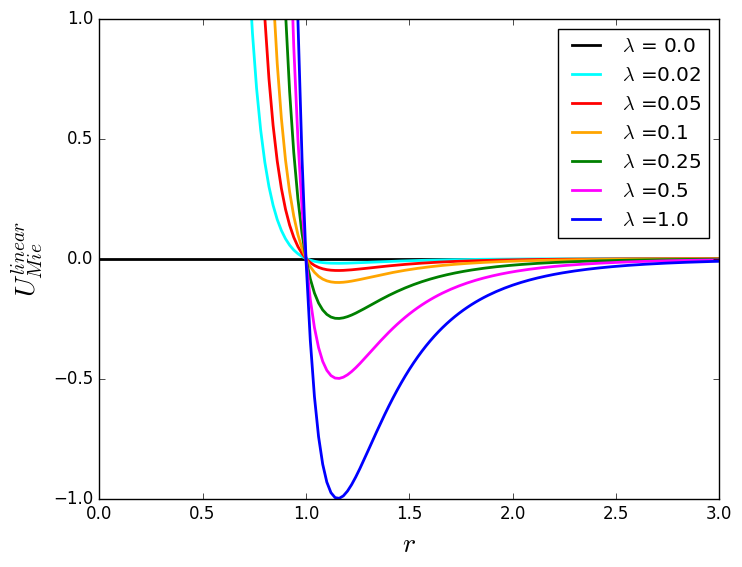
\includegraphics[width=0.8\linewidth]{Figures/linear8}
	\caption{\DIFaddFL{Linear coupling of the potential energy, $U^{linear}_{Mie} = \lambda U_{Mie}$, for different values of $\lambda$. Here, $\sigma=1$, $\epsilon=1$, $\lambda _a = 6$, and $\lambda _r = 8$.}}
	\label{fig:linearpoten}
\end{figure} 

\DIFadd{Observing Figure \ref{fig:linearpoten}, we can see }\DIFaddend that a linear coupling of the parameter would cause an abrupt change in the potential energy when the $\lambda$ reaches zero. That is the reason the non-linear softcore scheme \cite{beutler1994} is used to couple the $\lambda$. This scheme makes the potential behave more smoothly in relation to the change of $\lambda$\DIFdelbegin \DIFdel{, as can be seen in }%DIFDELCMD < \figref{fig:SC}%%%
\DIFdelend . The softcore potential is \DIFaddbegin \DIFadd{equal to
}\DIFaddend 

\begin{equation}
\label{eq:softcoreLJ}
\begin{aligned}
U_{LJ}^{sc}(r) {}=& 4\lambda\epsilon \left\lbrace\frac{1}{\left[\alpha(1-\lambda)+ (r/\sigma)^{6}\right]^{2}} - \frac{1}{\alpha(1-\lambda)+(r/\sigma)^{6}}\right\rbrace ,
\end{aligned}
\end{equation}
where $\alpha$ is a constant whose value is  normally assumed to be 0.5.    Based on Eq. \ref{eq:softcoreLJ}, we propose a generalized softcore Mie potential for any value of $\lambda _{r}$ and $\lambda _{a}$. It is given by:

\begin{equation}
\label{eq:softcore}
\DIFdelbegin %DIFDELCMD < \begin{aligned}
%DIFDELCMD < U^{sc}(r) {}=& \lambda\epsilon\dfrac{\lambda_r}{\lambda_r - \lambda_a} \left(\frac{\lambda_r}{\lambda_a} \right)^{\left( \frac{\lambda_a}{\lambda_r - \lambda_a} \right)} \left\lbrace\dfrac{1}{\left[\alpha(1-\lambda)+ (r/\sigma)^{\lambda_a}\right]^{\lambda_{r}/\lambda_{a}}} - \dfrac{1}{\alpha(1-\lambda)+(r/\sigma)^{\lambda_a}}\right\rbrace .
%DIFDELCMD < \end{aligned}
%DIFDELCMD < %%%
\DIFdelend \DIFaddbegin \begin{aligned}
U_{Mie}^{sc}(r) {}=& \lambda\epsilon\dfrac{\lambda_r}{\lambda_r - \lambda_a} \left(\frac{\lambda_r}{\lambda_a} \right)^{\left( \frac{\lambda_a}{\lambda_r - \lambda_a} \right)} \left\lbrace\dfrac{1}{\left[\alpha(1-\lambda)+ (r/\sigma)^{\lambda_a}\right]^{\lambda_{r}/\lambda_{a}}} - \dfrac{1}{\alpha(1-\lambda)+(r/\sigma)^{\lambda_a}}\right\rbrace .
\end{aligned}
\DIFaddend \end{equation}

\DIFdelbegin %DIFDELCMD < \begin{figure}[H]
%DIFDELCMD < 	%%%
\DIFdelendFL \DIFaddbeginFL \DIFaddFL{With the intention of observing the behavior of this generalized softcore potential, we plotted the $U_{Mie}^{sc}(r)$ with repulsive exponents of different hardness/softness for a range of values of $\lambda$ in Figures \ref{fig:scmie8} to \ref{fig:scmie30}. We see that this softcore scheme makes the potential behave more smoothly in relation to the change of $\lambda$, mainly for the softer repulsive exponents. 
}


%DIF > \begin{figure}
%DIF > 	\centering
%DIF > 	\subfloat[][]{%
%DIF > 		\label{fig:ex3-a}%
%DIF > 		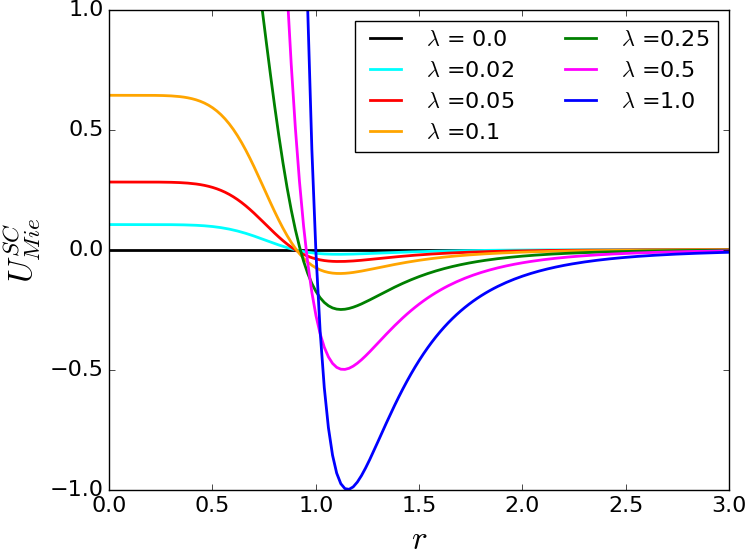
\includegraphics[height=5.9cm]{Figures/soft8}}%
%DIF > 	\hspace{0.05cm}%
%DIF > 	\subfloat[][]{%
%DIF > 		\label{fig:ex3-b}%
%DIF > 		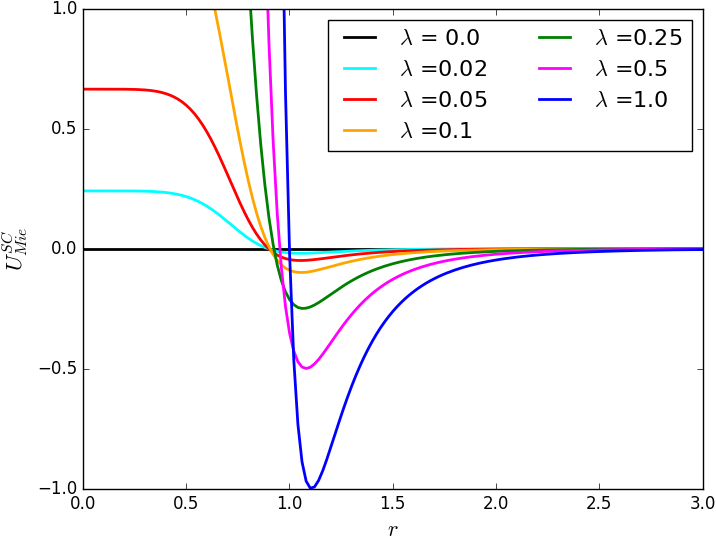
\includegraphics[height=5.9cm]{Figures/soft15}} \\
%DIF > 	
%DIF > 	\subfloat[][]{%
%DIF > 		\label{fig:ex3-c}%
%DIF > 		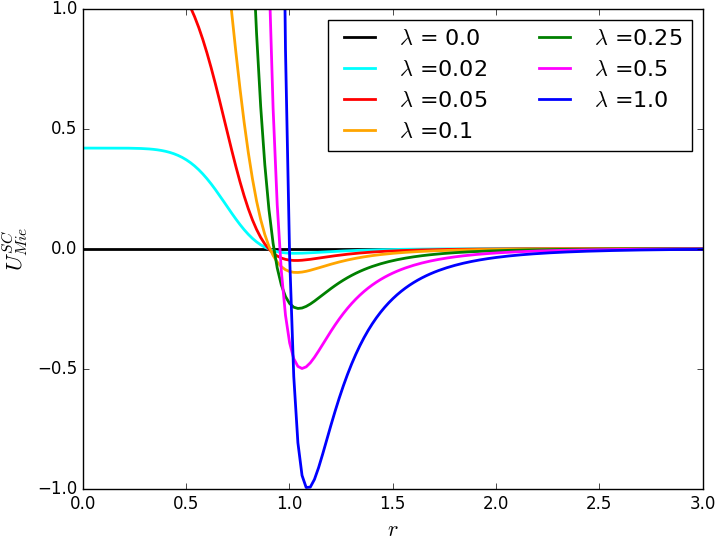
\includegraphics[height=5.9cm]{Figures/soft20}}%
%DIF > 	\hspace{0.05cm}%
%DIF > 	\subfloat[][]{%
%DIF > 		\label{fig:ex3-d}%
%DIF > 		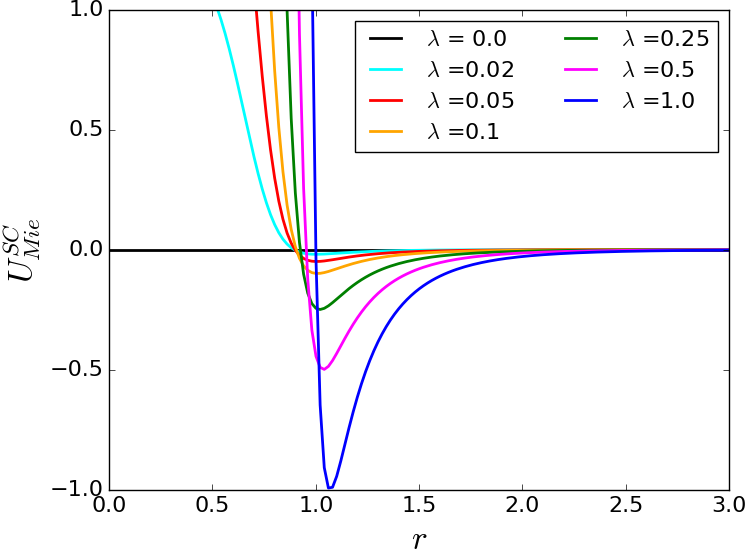
\includegraphics[height=5.9cm]{Figures/soft30}}%
%DIF > 	\caption[Generalized softcore Mie potential, Eq. \ref{eq:softcore}, for different values of $\lambda$.]{Generalized softcore Mie potential, Eq. \ref{eq:softcore}, for different values of $\lambda$. Here, $\sigma=1$, $\epsilon=1$, $\lambda _{a} = 6$, and $\lambda _{r}$ is equal to
%DIF > 		8 \subref{fig:ex3-a};
%DIF > 		15 \subref{fig:ex3-b};
%DIF > 		20 \subref{fig:ex3-c}; and,
%DIF > 		30 \subref{fig:ex3-d}.}%
%DIF > 	\label{fig:scmie}
%DIF > \end{figure}

\begin{figure}
	\DIFaddendFL \centering
		\DIFdelbeginFL %DIFDELCMD < 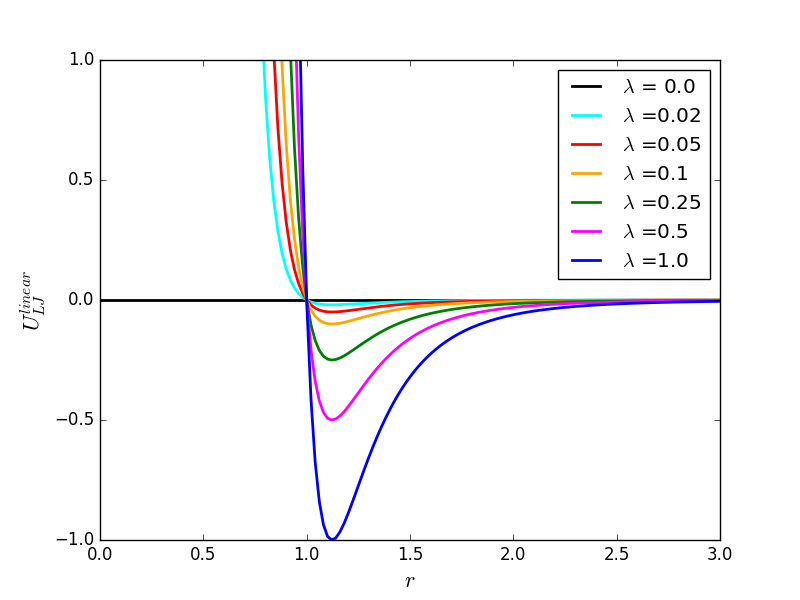
\includegraphics[width=0.8\linewidth]{Figures/linear}
%DIFDELCMD < 	%%%
\DIFdelendFL \DIFaddbeginFL 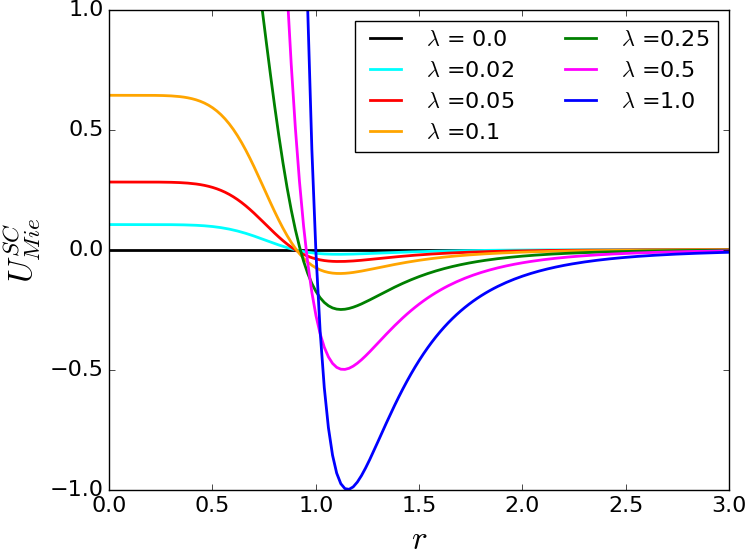
\includegraphics[width=0.8\linewidth]{Figures/soft8}%DIF > 
		\DIFaddendFL \caption{\DIFdelbeginFL \DIFdelFL{Linear coupling of the }\DIFdelendFL \DIFaddbeginFL \DIFaddFL{Generalized softcore Mie }\DIFaddendFL potential\DIFdelbeginFL \DIFdelFL{energy}\DIFdelendFL , \DIFdelbeginFL \DIFdelFL{$U^{linear}_{LJ} = \lambda U_{LJ}$}\DIFdelendFL \DIFaddbeginFL \DIFaddFL{Eq. \ref{eq:softcore}}\DIFaddendFL , for different values of $\lambda$. Here, $\sigma=1$\DIFdelbeginFL \DIFdelFL{and }\DIFdelendFL \DIFaddbeginFL \DIFaddFL{, }\DIFaddendFL $\epsilon=1$\DIFaddbeginFL \DIFaddFL{, $\lambda _{a} = 6$, and $\lambda _{r}=8$}\DIFaddendFL }
		\DIFdelbeginFL %DIFDELCMD < %DIFDELCMD < \label{fig:linearpoten}%%%
%DIFDELCMD < %%%
\DIFdelendFL \DIFaddbeginFL \label{fig:scmie8}
\DIFaddendFL \end{figure}

\DIFdelbegin %DIFDELCMD < \begin{figure}[H]
%DIFDELCMD < 	%%%
\DIFdelendFL \DIFaddbeginFL \begin{figure}
	\DIFaddendFL \centering
	\DIFdelbeginFL %DIFDELCMD < 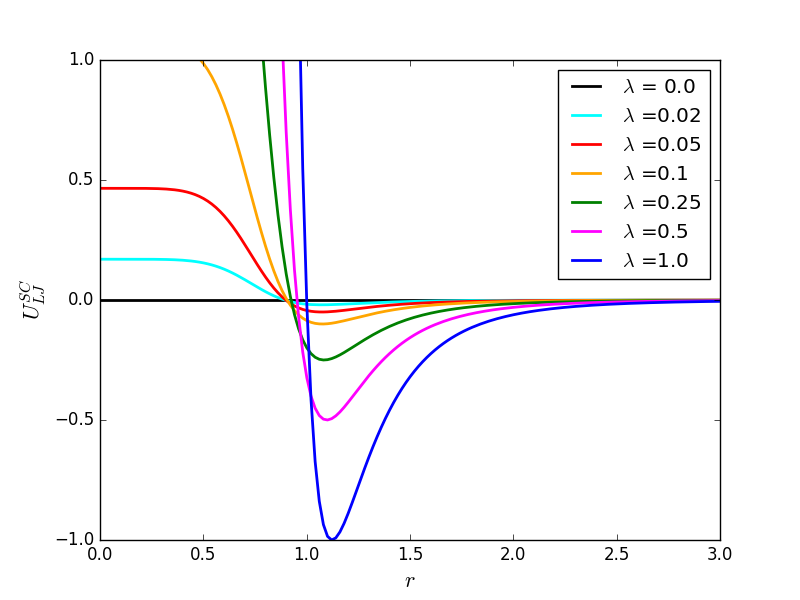
\includegraphics[width=0.8\linewidth]{Figures/soft}
%DIFDELCMD < 	%%%
\DIFdelendFL \DIFaddbeginFL 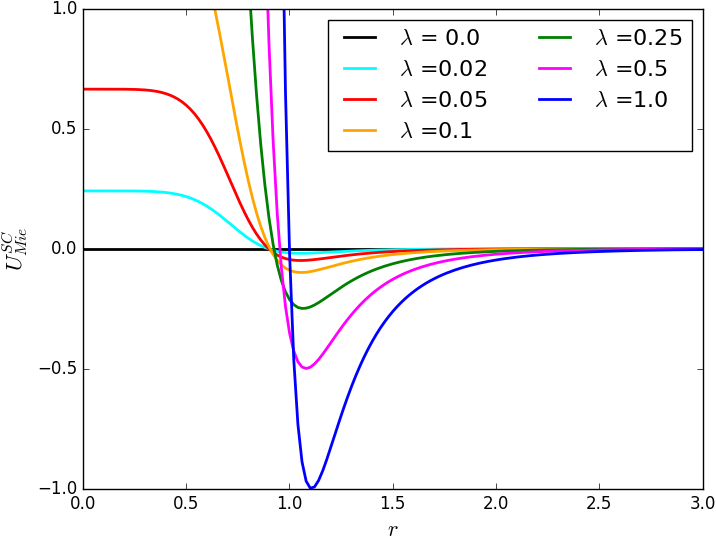
\includegraphics[width=0.8\linewidth]{Figures/soft15}%DIF > 
\DIFaddendFL \caption{\DIFdelbeginFL \DIFdelFL{Softcore }\DIFdelendFL \DIFaddbeginFL \DIFaddFL{Generalized softcore Mie }\DIFaddendFL potential, Eq. \DIFdelbeginFL \DIFdelFL{\ref{eq:softcoreLJ}}\DIFdelendFL \DIFaddbeginFL \DIFaddFL{\ref{eq:softcore}}\DIFaddendFL , for different values of $\lambda$. Here, $\sigma=1$\DIFdelbeginFL \DIFdelFL{and }\DIFdelendFL \DIFaddbeginFL \DIFaddFL{, }\DIFaddendFL $\epsilon=1$\DIFdelbeginFL \DIFdelFL{.}\DIFdelendFL \DIFaddbeginFL \DIFaddFL{, $\lambda _{a} = 6$, and $\lambda _{r}=15$}\DIFaddendFL }
\DIFdelbeginFL %DIFDELCMD < %DIFDELCMD < \label{fig:SC}%%%
%DIFDELCMD < %%%
\DIFdelendFL \DIFaddbeginFL \label{fig:scmie15}
\end{figure}

\begin{figure}
	\centering
	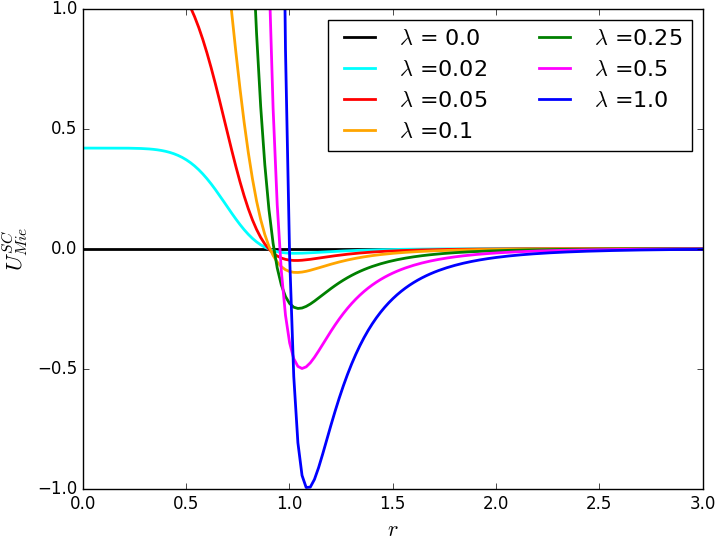
\includegraphics[width=0.8\linewidth]{Figures/soft20}%DIF > 
\caption{\DIFaddFL{Generalized softcore Mie potential, Eq. \ref{eq:softcore}, for different values of $\lambda$. Here, $\sigma=1$, $\epsilon=1$, $\lambda _{a} = 6$, and $\lambda _{r}=20$}}
\label{fig:scmie20}
\end{figure}

\begin{figure}
	\centering
	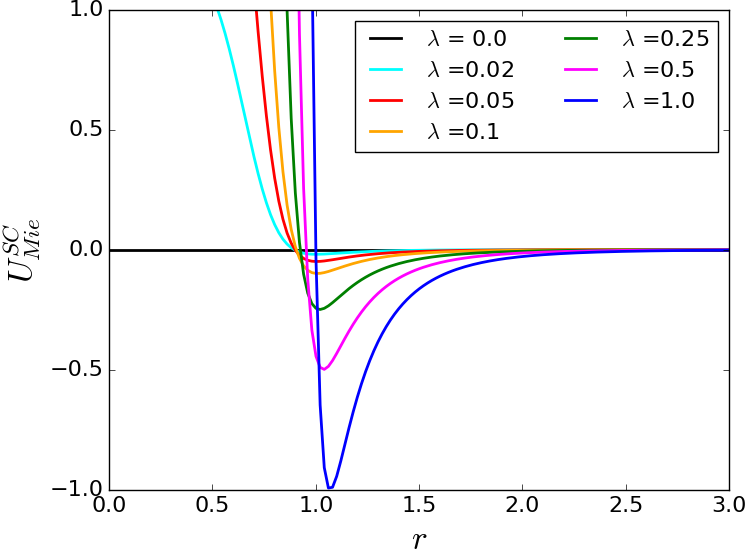
\includegraphics[width=0.8\linewidth]{Figures/soft30}%DIF > 
\caption{\DIFaddFL{Generalized softcore Mie potential, Eq. \ref{eq:softcore}, for different values of $\lambda$. Here, $\sigma=1$, $\epsilon=1$, $\lambda _{a} = 6$, and $\lambda _{r}=30$}}
\label{fig:scmie30}
\DIFaddendFL \end{figure}

\DIFaddbegin \FloatBarrier
\DIFaddend Now that we defined our coupled potential, we can then obtain the potential energies related to each alchemical state by doing independent simulations in different values of $\lambda$ or by doing expanded ensemble simulations \cite{lyubartsev}. The latter was the method used in this dissertation, and it is described in Section \ref{ee}. With the potential energies, the next step is to use post-processing methods, such as the MBAR used in this study, to effectively calculate $\Delta G_{3 \rightarrow 4}$.  The solvation free energies can then be used to calculate other properties such as the partition coefficient. This property is a measure of the partitioning of one solute in two solvents (a and b) with different physicochemical characteristics  at a temperature T. It is defined by the following equation when the activity coefficients are assumed to be one \cite{doi:10.1021/ja00036a009}:

\begin{equation}
P = \dfrac{[solute]_{a}}{[solute]_{b}},
\end{equation} 
where $[solute]_{a}$ and $[solute]_{b}$ are the concentration of the solute in the solvent a and b, respectively. Since $P$ is an equilibrium constant, it can be related to free energy change associated with transferring the solute from the phase a to the phase b. Hence, we can define the relation between the partition coefficient and the difference in free energy with the equation bellow \cite{doi:10.1021/ja00036a009}:  

\begin{equation}
\label{eqn:partcoe}
{2.303RT} \log{P}^{a/b} ={\Delta G_{solv}^{a} - \Delta G_{solv}^{b}},
\end{equation}
where 2.303 is a conversion factor.

\section{Expanded Ensemble Method}\label{ee}

We decided to use the Expanded Ensemble method \cite{lyubartsev} in our solvation free energy simulations since it allows a non-Boltzmann sampling scheme of different states in a single simulation. \citeonline{lyubartsev} initially proposed in their paper a sampling scheme of different temperatures, but this idea can be generalized to a sampling scheme of different states or $\lambda 's$ \cite{escobedo2007}. In this scheme, the sampling is done by biasing the phase space exploration process with weights not related to the statistical ensemble. The partition function of the statistical expanded ensemble, $Z^{EE}$, is obtained from the probability distributions corresponding to each $\lambda$. Hence, $Z^{EE}$ is defined as a sum of subensembles $Z_{i}$ in different values of $\lambda$, that is,

\begin{equation}
Z^{EE} = \sum_{i=1}^{N} Z_{i}(\lambda_{i}) exp(\eta_{i}),
\label{eqn:ee}
\end{equation}   
where N is the number of alchemical states, $\eta_{i}$ is the arbitrary weight of the subensemble at each state, and $Z_{i}$ is the configurational partition function of state i. For the isothermal-isobaric ensemble, $Z_{i}$ is given by

\begin{equation}
Z_{i} = \frac{1}{V_{0}} {\int_{0}^{\infty} dV \int \DIFdelbegin \DIFdel{d^{n}r}\DIFdelend \DIFaddbegin \DIFadd{dr}\DIFaddend ^{n} \exp \left \lbrace -\beta_{i} \left[ U(\lambda, r_{1},..,r_{n}) + P_{i}V(r_{1},..,r_{n}) \right] \right \rbrace}.
\end{equation} 

In solvation free energy calculations with molecular dynamics, $\lambda$ corresponds to the coupling parameter of the softcore potential (Eq. \ref{eq:softcoreLJ}). Since we are carrying out molecular dynamic simulations, the sampling of the expanded ensemble is done by performing an arbitrary number of MD  steps followed by a $\lambda$ transition. \citeonline{chodera2011} proved that this type of sampling of the expanded ensemble is similar to the Gibbs sampling method \cite{geman1984,liu2002}. Following the Gibbs method, the sampling of the configuration space $x$ for one state $\lambda_{k}$ during the MD steps is done by using the conditional distribution:

\begin{equation}
\pi(x|\lambda_{k}) = \dfrac{\exp[-\beta u(x,\lambda_{k})]}{\int dx \exp [- \beta u(x,\lambda_{k})]}.
\label{eqn:rhoee1}
\end{equation} 

The state transition in the MD simulation uses the following conditional distribution:

\begin{equation}
\pi(\lambda_{k}|x) = \dfrac{\exp[-\beta u(x,\lambda_{k}) + \eta_{k}]}{ \sum_{k=1}^{K} \exp [- \beta u(x,\lambda_{k})+ \eta_{k}]},
\label{eqn:rhoee2}
\end{equation} 
where $u(x,\lambda_{k})$ is the reduced potential function for the NPT ensemble. There is a variety of acceptance schemes to do the expanded sampling using Eq. \eqref{eqn:rhoee2}, but \citeonline{chodera2011} suggested that the independence sampling \cite{liu2002} is the best strategy to increase the number of uncorrelated configurations. The implementation they suggested consists of updating the state index from $i$ to $j$ by first generating a uniform random number $R$ on the interval $[0,1)$ and then selecting the smallest new value of $j$ that satisfies  the relation

\begin{equation}
R < \sum_{i=1}^{j} \pi(\lambda_{i}|x) .
\label{eqn:relee2}
\end{equation} 

The sampling strategy above depends on a proper selection of weights in order to guarantee an adequate sampling of the states. If there is not a sufficient number of visits to each state, the expanded ensemble becomes deficient in obtaining input data to estimate free energy differences with the methods exposed in Section \ref{SFECM}. Here, we followed the flat-histogram approach \cite{bernd1992,bernd1993,dayal2004} to calculate the weights. This strategy aims to obtain adequate sampling by ensuring that all the states have an equal number of visits, i.e.\DIFaddbegin \DIFadd{, }\DIFaddend the ratio of the probability of sampling state i ($\pi_{i}$) to the probability of sampling state $j$ ($\pi_{j}$) is equal to one. Given that $\pi_{i}$ is equal to:

\begin{equation}
\pi_{i} = \dfrac{Z_{i}(\lambda_{i}) exp(\eta_{i})}{Z^{EE}} ,
\label{eqn:wei1}
\end{equation} 

\DIFdelbegin %DIFDELCMD < {%%%
\DIFdelend Substituting Eq. \ref{eq:dif} in Eq. \ref{eqn:wei1}, the following relation can be obtained for $\pi_{i}/\pi_{j}=1$:

\begin{equation}
(\eta_{i} - \eta_{j}) = \beta(G_i-G_j).
\label{eqn:weight}
\end{equation}

Eq. \eqref{eqn:weight} proposes that the choice of the weights is dependent on the free energies that we are attempting to obtain. This equation is then solved iteratively with trial simulations. For the first simulation, the values of $\eta$ are set to zero, and the histogram of the states visited is obtained. With this histogram, it is possible to estimate the free energy differences and, since the weights are related to the free energies by Eq. \eqref{eqn:weight}, the next values of $\eta$ can be calculated. This iteration goes on until a uniform distribution is attained. The weights found are then used in a longer simulation to obtain the final solvation free energies.

The choice of the $\lambda$ set corresponding to overlapping alchemical states are crucial to acquire accurate solvation free energies. In this work, the method chosen to obtain the optimal staging of the $\lambda$ domain is the one developed by \citeonline{escobedo2007} with a basis in the study of  \citeonline{1742-5468-2006-03-P03018}. This method targets "bottlenecks" in the simulation. It does that by optimizing $\lambda$ through the minimization of the number of round trips per CPU time between the lowest ($0$) and highest ($1$) values of $\lambda$. This is specifically done by maximizing the steady-state flow $\phi$ of the simulation, which "walks" among the values of $\lambda$. This flow is estimated from a Fick's diffusion type of law:

\begin{equation}
\phi = D(\Lambda) \Pi (\Lambda) \dfrac{dx(\Lambda)}{d \Lambda}.
\label{eqn:stream}
\end{equation}

In the equation above, $\Lambda$ is the actual continuous value of the coupling parameter. This continuous function of $\lambda 's$ is obtained by interpolating the $\lambda$ set linearly. $D(\Lambda)$ is the diffusivity at  state $\Lambda$ and $x(\Lambda)$ is the fraction of times that the trial simulation at state $\Lambda_{i}$ has most recently visited the state $\lambda=1$ as opposed to state $\lambda=0$. The derivative ${dx(\Lambda)}/{d \Lambda}$ is approximated with the central finite differences method. Finally, $\Pi (\Lambda)$ is the probability of visiting $\Lambda$:

\begin{equation}
\Pi (\Lambda) = \dfrac{C^{'} \bar{\Pi} (\lambda)}{\Lambda_{i+1} - \Lambda_{i}}.
\label{eqn:plambda}
\end{equation}

The $C^{'} $ term in the equation above represents a constant and $\bar{\Pi} (\lambda)$ is the arithmetic average of the frequency of visits to the $\Lambda$ state:

\begin{equation}
\bar{\Pi}_{i} (\lambda) = \dfrac{\pi_{i+1} - \pi_{i}}{2}.
\label{eqn:barplambda}
\end{equation}

The $\phi$ is maximum when the optimal probability $\Pi^{'}(\Lambda_{i})$ of visiting state $\Lambda_{i}$ is proportional to $1/\sqrt{D(\Lambda)}$ \cite{trebst2004}. With that information, it is possible to estimate the diffusivity using one trial simulation with the following equation:

\begin{equation}
\begin{aligned}
D(\Lambda) {}=& \dfrac{\Lambda_{i+1} - \Lambda_{i}}{\bar{\Pi} (\lambda) {dx(\Lambda)}/{d \Lambda}}, \quad \Lambda_{i} < \Lambda < \Lambda_{i+1}.
\end{aligned}
\label{eqn:diff}
\end{equation}    
Hence, we can calculate $\bar{\Pi} $ and, consequently, the cumulative probability, which is used to obtain the new $\lambda$ states by

\begin{equation}
\Phi = \int_{\lambda =0}^{\lambda =1} \Pi^{'}(\Lambda_{i}) d \Lambda = \dfrac{i}{K},
\label{eqn:cumfun}
\end{equation}
where $K$ is the total number of $\lambda$ states. In order to carry out our solvation free energy simulations, we obtained these cumulative probabilities for every $\lambda$ set we estimated. A graphical demonstration of the relation between the optimized coupling parameters and the cumulative probability of Eq. \ref{eqn:cumfun} is presented in Figure \ref{fig:optimized_cdfexeample}.

\begin{figure}[h]
	\centering
	\DIFdelbeginFL %DIFDELCMD < 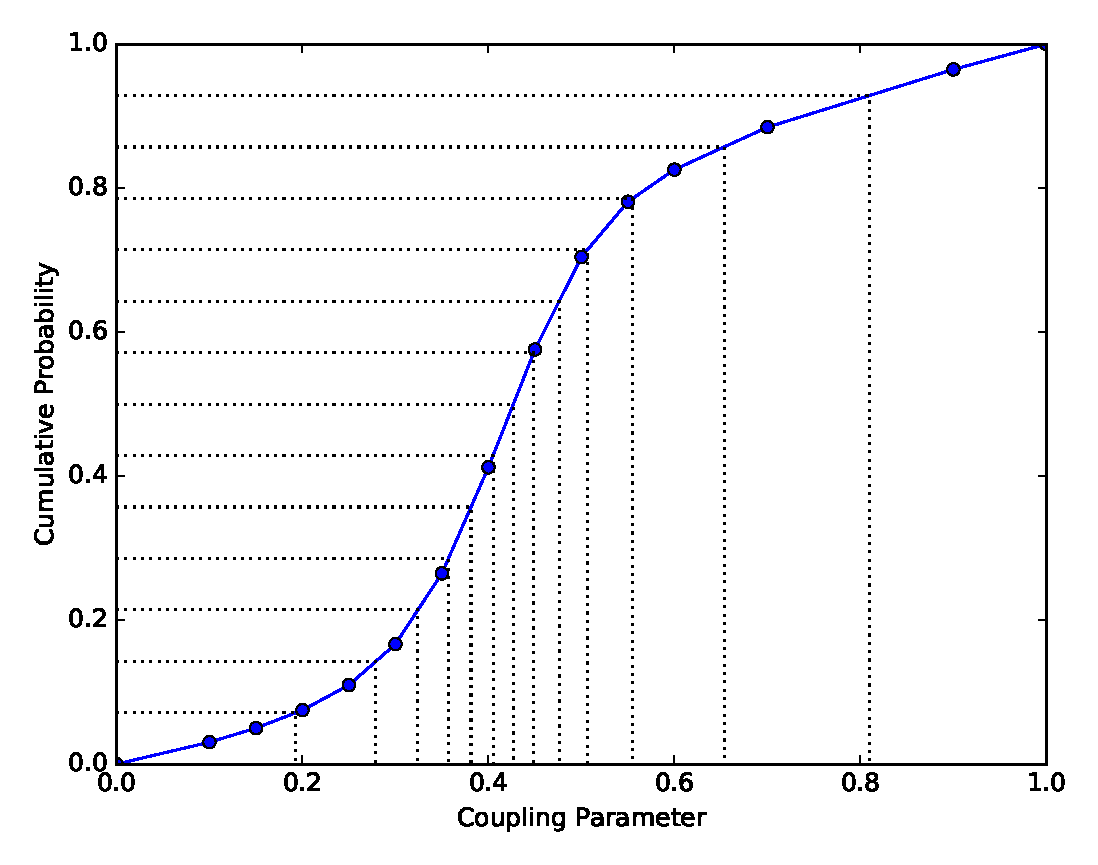
\includegraphics[width=0.8\linewidth]{Figures/optimized_cdfexeample}
%DIFDELCMD < 	%%%
\DIFdelendFL \DIFaddbeginFL 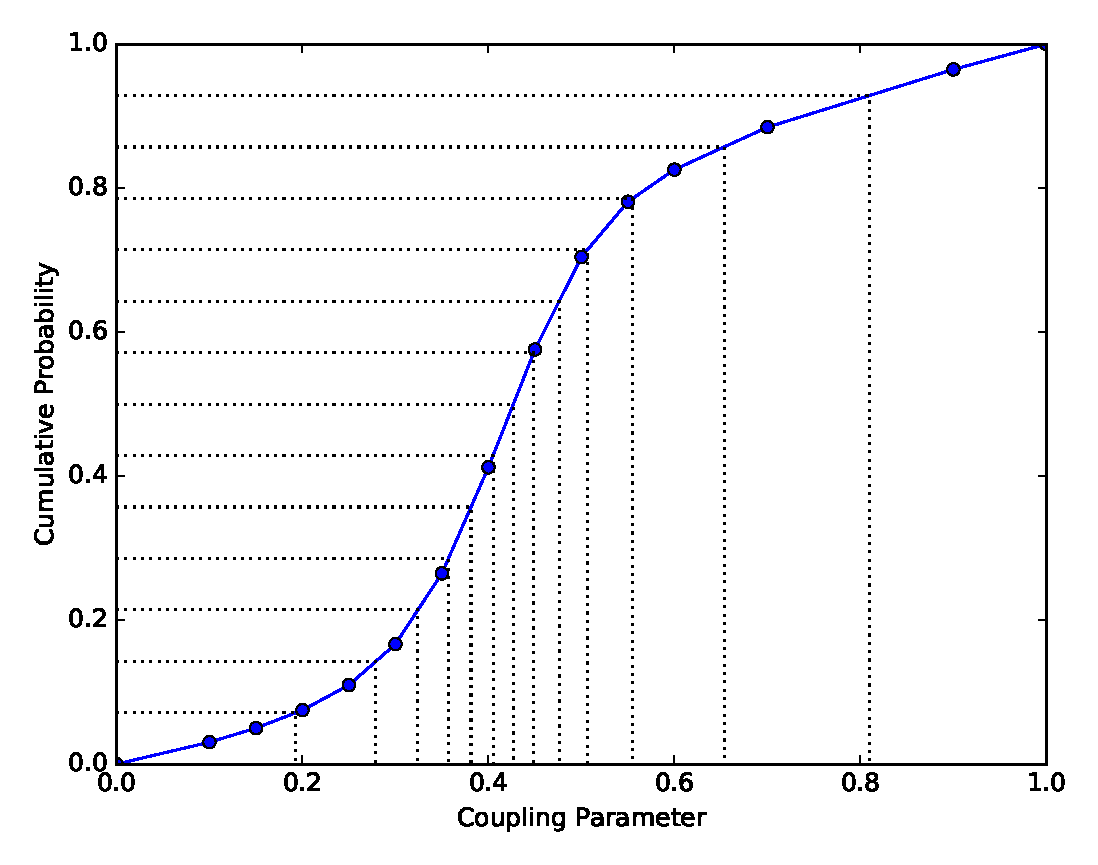
\includegraphics[width=0.75\linewidth]{Figures/optimized_cdfexeample}
	\DIFaddendFL \caption{Relation between the optimized coupling parameters and the cumulative probability used to obtain them.}
	\label{fig:optimized_cdfexeample}
\end{figure}
\FloatBarrier
\section{Multistate Bennett Acceptance Ratio (MBAR)}\label{mbar}

We presented in the sections above the methods used to obtain the total potential energies of each alchemical state with molecular dynamics, and, in this section, we are going to discuss the methodology utilized to estimate the solvation free energies with these data. The MBAR method \cite{mbar} is based on the free energy perturbation. It is a maximum likelihood method which computes free energies and their uncertainties of all $K$ states by minimizing the $K \times K$ matrix of variances for a simulation with $N_{j}$ uncorrelated samples in equilibrium. For each of the $\lbrace x_{i,n } \rbrace ^{N_{i}}_{n=1 }$ configurations of i, the following probability distributions are sampled:
\begin{equation}
p_{i}(x) = \frac{q_{i}(x)}{c_{i}},
\end{equation}

\begin{equation}
c_{i} = \int dx q_{i}(x),
\end{equation}
where $q_{i}(x)=\exp[-u_{i}(x)]$ and $u_{i}$ is the reduced potential energy of each state, defined for a an alchemical transformation by $u_{i} (x)= \beta_{i} [U_{i}(x)]$. In addition, $c_{i}$ is a normalization constant.  The free energies are estimated from the ratio of this constant in each state, since

\begin{equation}
\Delta f_{ij} = f_{i} - f_{j} = - \ln \frac{c_{j}}{c_{i}}  = -\ln \frac{\int dx q_{j}(x)}{\int dx q_{i}(x)} .
\label{eqn:mbar1}
\end{equation}

\citeonline{mbar} then proposed the following arbitrary function:

\begin{equation}
c_{i} \langle \alpha _{ij} q_{j} \rangle _{i}  =  c_{j} \langle \alpha _{ij} q_{i} \rangle _{j} .
\end{equation}

Using the equation above for every state  K, the following relation is obtained:

\begin{equation}
\label{eq:mbar1}
\sum_{j=1}^{K} \frac{\hat{c_{i}}}{N_{i}} \sum_{n=1}^{N_{i}} \alpha _{ij} q_{j} (x_{i,n}) =  \sum_{j=1}^{K} \frac{\hat{c_{j}}}{N_{j}} \sum_{n=1}^{N_{j}} \alpha _{ij} q_{i} (x_{j,n}) .
\end{equation}

\citeonline{mbar} suggested the following equation for the arbitrary term $\alpha _{ij}$ in order to minimize the variance:

\begin{equation}
\label{eq:mbar2}
\alpha _{ij} (x) = \frac{N_{j} \hat{c_{i}} ^{-1}}{\sum_{k=1}^{K} N_{k} c_{i} ^{-1} q_{k}(x)} .
\end{equation}

Assuming that the sampling is carried out following Boltzmann statistics, Eqs. \eqref{eq:mbar1} and \eqref{eq:mbar2} can be rearranged to obtain the free energy estimator, which is solved self consistently:  

\begin{equation}
\label{eq:mbar}
\DIFdelbegin %DIFDELCMD < \begin{aligned}
%DIFDELCMD < f_{i} = \frac{1}{\beta}ln \sum_{k=1}^{K} \sum_{n=1}^{N_{k}}
%DIFDELCMD < \dfrac{\exp[-\beta u_{i}(x_{kn})]}{\sum_{l=1}^{K} N_{l} \exp \lbrace \beta [f_{l} - u_{l}(x_{kn})] \rbrace} .
%DIFDELCMD < \end{aligned}
%DIFDELCMD < %%%
\DIFdelend \DIFaddbegin \begin{aligned}
f_{i} = -ln \sum_{k=1}^{K} \sum_{n=1}^{N_{k}}
\dfrac{\exp[- u_{i}(x_{kn})]}{\sum_{l=1}^{K} N_{l} \exp \lbrace  [f_{l} - u_{l}(x_{kn})] \rbrace} .
\end{aligned}
\DIFaddend \end{equation}

The equation above requires the evaluation of the potential energy  of every  uncorrelated configuration $n$ for all K states [$u_{i}(x_{kn})$] and for all uncorrelated configuration snapshots ($N_{k}$) from state $k$. With the free energies, we compute the free energy differences between states with Eq. \ref{eqn:mbar1}. The uncertainty resulting from free energy estimation can be computed by the covariance matrix ($s$):

\begin{equation}
\DIFdelbegin %DIFDELCMD < \begin{aligned}
%DIFDELCMD < \delta _{ij}^{2} s_{ij} = s_{ii}^{2} + s_{jj}^{2} - 2 s_{ij}.
%DIFDELCMD < \end{aligned}
%DIFDELCMD < %%%
\DIFdelend \DIFaddbegin \begin{aligned}
\delta _{ij}^{2} \Delta f _{ij} = s_{ii} + s_{jj} - 2 s_{ij}.
\end{aligned}
\DIFaddend \end{equation}

The MBAR method explained here can be considered as a limiting case of the 
Weighted Histogram Analysis Method (WHAM) \cite{wham} for computing free energies. WHAM equations become equal to Eq. \eqref{eq:mbar} if the histogram width tends to zero. Despite this, the MBAR is still more suited than the WHAM because it does not have the bias associated with the discretization and allows the calculation of an error estimate \cite{mbar}.

\section{Gibbs Ensemble Monte Carlo (GEMC)}\label{gemc}

In the initial steps of this research, we estimated the SAFT-$\gamma$ Mie force field parameters of phenanthrene with the methodology proposed by \citeonline{lafitte2012}. This approach required liquid-vapor equilibrium data obtained with molecular simulation, as it is described in Section \ref{parsaft}. Hence, we carried out Monte Carlo simulations at the Gibbs Ensemble \cite{papa1987} since this ensemble is commonly used to study phase coexistence with molecular simulation. In addition to that, this method does not use an explicit interface, which can hinder the determination of bulk phase behavior of small systems with long-range interactions \cite{C1FD00090J}. 

Before talking in more detail about this ensemble, we are going to discourse on Monte Carlo simulations briefly. The Monte Carlo (MC) approach is another method for generating atomic trajectories in order to obtain macroscopic properties. Rather than using the numerical integration of Newton's equations of motion, the trajectories are obtained stochastically in the Monte Carlo approach. The positions are evolved by random moves or perturbations (MC steps) acquired with the Metropolis method \cite{1953JChPh..21.1087M}. Hence, the trajectories are not predictable from the set of initial positions. The Metropolis method is a Markov process, that is, a stochastic process in which the configurations change randomly with time and only depends on the states and their directly preceding states, but not on the previous configurations \cite{raabe}. The random move is constructed in such a way that the probability of visiting a particular point $r^{N}$ is proportional to the Boltzmann factor $exp[-\beta U(r^{N})]$ \cite{frenkel}. The construction of a  particle displacement according to \citeonline{1953JChPh..21.1087M} can be briefly summed up as:

1. Pick a random particle, and calculate its energy $U(r^{N})$.

2. Perturb the particle by randomly displacing  it, $r' = r +\Delta r$. Where $\Delta r$ is a perturbation randomly chosen from a defined interval of maximum displacement ($[- \delta _{max},\delta _{max}]$). Calculate the energy with the new positions $U(r'^{N})$.

3. Accept the move from $r^{N}$ to $r'^{N}$ with the probability:
\begin{equation}
acc_{A \rightarrow B} = min \lbrace 1,exp[-\beta U(r'^{N}) + \beta U(r^{N}) ] \rbrace .
\end{equation}

The values of maximum displacement are defined iteratively in order to obtain acceptance rates of 25-50\% in step 3   \cite{Frenkel2013}. Monte Carlo simulations are interesting when we need to calculate properties in different thermodynamic ensembles, such as the Gibbs Ensemble used in this dissertation. The phase coexistence at this ensemble is obtained with simultaneous Monte Carlo (MC) simulations of two boxes with periodic boundary conditions, representing a two-phase system. The boxes exchange molecules, energy, and volume between them. Equilibrium is obtained through MC steps that consist of translation and rotation moves, volume exchange moves, and random exchanges of molecules between the boxes. For the phase equilibrium of multi-component systems, the GEMC simulations should be carried out at the NPT (constant number of particles, pressure, and temperature) ensemble to obey the requirement of an additional degree of freedom for mixtures. In turn, the simulation of single component systems is carried out at a constant number of particles, temperature, and volume (NVT) since the two-phase region would be a line for this system at constant pressure and temperature \cite{frenkel}. The partition function of the GEMC-NVT ensemble is obtained by considering that the particles in both boxes are subjected to the same intermolecular interactions. Also, volumes and number of particles of the box ($N_{1}$,$\, N_{2}$,$\, V_{1}$ and $V_{2}$) can vary while the total volume ($V$) and the total number of particles ($N$) remain constant ($N = N_{1} + N_{2}$,$\, V = V_{1} + V_{2}$). Therefore, the partition function is

\begin{equation}
\begin{aligned}
Q(NVT) {} \equiv & \sum_{N_{1}}^{N} \dfrac{1}{V \Lambda ^{3N} N_{1}!(N-N_{1})!} \int_{0}^{V} V_{1}^{N_{1}} V_{2}^{N_{2}} dV_{1} \\
& \int  \exp[-\beta U(x_{1}^{N_{1}})] dx_{1}^{N_{1}} \int  \exp[-\beta U(x_{2}^{N_{2}})] dx_{2}^{N_{2}}.
\end{aligned}
\label{eqn:gepart}
\end{equation}

In order to define the acceptance rules for the MC moves and compute any property of interest, it is necessary to know the probability of finding the configuration with $N_{1}$ particles in box 1 with volume $V_{1}$ and positions $x_{1}^{N_{1}}$ and $x_{2}^{N_{2}}$. This probability is given by:

\begin{equation}
\pi(x_{1}^{N_{1}},x_{2}^{N_{2}},N_{1},N_{2},V_{1},V_{2}) \propto \dfrac{V_{1}^{N_{1}}V_{2}^{N_{2}}}{N_{1}!N_{2}!} \DIFdelbegin \DIFdel{\exp[-\beta U(x_{1}^{N_{1}}) -\beta U(x_{2}^{N_{2}})] }\DIFdelend \DIFaddbegin \DIFadd{\exp[-\beta U(x_{1}^{N_{1}}) +\beta U(x_{2}^{N_{2}})] }\DIFaddend .
\label{eqn:geprob}
\end{equation}

The acceptance criterion for the translation and rotation moves from configuration A    to configuration B is similar to the conventional NVT MC method and is equal to:

\begin{equation}
acc_{A \rightarrow B} = \min \lbrace 1,\DIFdelbegin \DIFdel{\exp[-\beta U(x_{A}^{N_{1}}) -\beta U(x_{B}^{N_{1}})] }\DIFdelend \DIFaddbegin \DIFadd{\exp[\beta U(x_{A}^{N_{1}}) -\beta U(x_{B}^{N_{1}})] }\DIFaddend \rbrace .
\label{eqn:drprob}
\end{equation} 

The volume exchange moves take place by exchanging an amount $\Delta V$ between the boxes to achieve pressure equilibrium. $\Delta V$ can be chosen from a uniform distribution based on the maximum variation of volume ($\delta V_{max}$) defined with probability $1/\delta V_{max}$ \cite{frenkel}. The acceptance rule for these moves is: 

\begin{equation}
acc_{A \rightarrow B} = \min \left \lbrace 1, \left(\dfrac{V_{1}^{B}}{V_{1}^{A}} \right)\DIFdelbegin \DIFdel{^{N_{1}=1} }\DIFdelend \DIFaddbegin \DIFadd{^{N_{1}+1} }\DIFaddend \left( \dfrac{V_{2}^{B}}{V_{2}^{A}} \right)^{N_{2}+1} \DIFdelbegin \DIFdel{\exp[-\beta U(x_{A}^{N}) -\beta U(x_{B}^{N})] }\DIFdelend \DIFaddbegin \DIFadd{\exp[\beta U(x_{A}^{N}) -\beta U(x_{B}^{N})] }\DIFaddend \right \rbrace .
\label{vprob}
\end{equation}

Particle exchange moves are carried out to obtain the equality of chemical potential between the boxes. One particle from one box is removed and then added to a random location in the other box. The criteria to accept or reject this type of move is:

\begin{equation}
acc_{A \rightarrow B} = \min \left \lbrace 1, \DIFdelbegin %DIFDELCMD < \dfrac{N_{1}V_{2}}{N_{2}V_{1}}  %%%
\DIFdel{\exp[-\beta U(x_{A}^{N}) -\beta U(x_{B}^{N})] }\DIFdelend \DIFaddbegin \dfrac{N_{1}V_{2}}{(N_{2}+1)V_{1}}  \DIFadd{\exp[ \beta U(x_{A}^{N}) -\beta U(x_{B}^{N})] }\DIFaddend \right \rbrace .
\label{moleprob}
\end{equation}

This method has been widely used to calculate phase equilibrium, but its performance is poor for the region near the critical point due to large density fluctuations. The GEMC method also has poor performance for dense systems since the particle exchange moves have a low acceptance rate \cite{978-94-017-0765-7}.  






\chapter{Methodology} % Main chapter title

\label{Chapter4} % Change X to a consecutive number; for referencing this chapter elsewhere, use \ref{ChapterX}

In this study, we had first to obtain the parameters of phenanthrene using an equation for rings for the SAFT-$\gamma$ Mie force field since these parameters were not available on this force field database \cite{ervik2016}. Hence, we divided this chapter into two sections. The first one describes how we parametrized the phenanthrene molecule with the SAFT-$\gamma$ Mie force field and the second one explains how we carried out the solvation free energy simulations. 

\section{Phenanthrene Parameterization}\label{parame}

We implemented the two parameterization strategies for molecules with aromatic rings described in Section \ref{parsaft} for phenanthrene. For both of them, only vapor pressure data \DIFdelbegin \DIFdel{\mbox{%DIFAUXCMD
\cite{pvphen} }%DIFAUXCMD
}\DIFdelend \DIFaddbegin \DIFadd{\mbox{%DIFAUXCMD
\cite{pvphen,osborn} }%DIFAUXCMD
}\DIFaddend were used due to the unavailability of saturated liquid density. We did not estimate the attractive exponent, $\lambda _{a}$. Instead, the value of six was given to it, as recommended by \citeonline{ramrattan2015} and \citeonline{herdes2015}, due to its high correlation with the repulsive exponent. The parameterization with the ring equation of \citeonline{muller2017} was carried out with the number of segments equal to five and with a geometry such as that in \figref{fig:fen5}, since this level of coarse-graining was also used for a similar molecule (anthracene) in the original paper.
\begin{figure}[th]
	\centering
	\DIFdelbeginFL %DIFDELCMD < 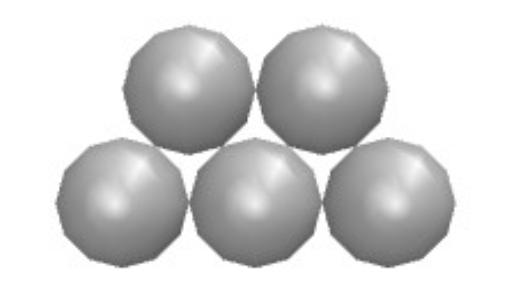
\includegraphics[width=0.25\linewidth]{Figures/fen5}
%DIFDELCMD < 	%%%
\DIFdelendFL \DIFaddbeginFL 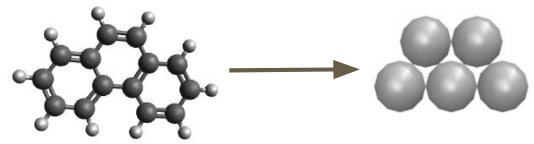
\includegraphics[width=0.70\linewidth]{Figures/fe5cg}
	\DIFaddendFL \caption{Representation of phenanthrene with the geometry proposed by \citeonline{muller2017}. }
	\label{fig:fen5}
\end{figure}

The minimization was done using the Particle Swarm Optimization (PSO)  method \cite{pso} with \DIFdelbegin \DIFdel{the following objective function :
}\DIFdelend \DIFaddbegin \DIFadd{50 particles and 50 interactions. The objective function used was equal to
}\DIFaddend \begin{equation}
\DIFdelbegin \DIFdel{\min}%DIFDELCMD < \limits%%%
\DIFdel{_{\sigma,\epsilon,\lambda_{r}} }\DIFdelend F_{obj} = \sum_{i=1}^{N_{p}} \left[\frac{P_{v}^{SAFT}(T_{i},\sigma,\epsilon,\lambda_{r})-P_{v}^{exp}(T_{i})}{P_{v}^{exp}(T_{i})} \right]^2 .
\label{eqn:fobjm}
\end{equation}

Here, $P_{v}^{exp}$ is the experimental vapor pressure and $P_{v}^{SAFT}$ is the vapor pressure obtained with the SAFT-VR Mie EoS. \DIFdelbegin \DIFdel{We used the routine proposed by
\mbox{%DIFAUXCMD
\citeonline{smithbook} }%DIFAUXCMD
}\DIFdelend \DIFaddbegin \DIFadd{According to the fundamental thermodynamic equation, the vapor pressure is given by
}\begin{equation}
\DIFadd{P_{v}^{SAFT} =  - \frac{\partial A^{SAFT}}{\partial V}
}\end{equation}

\DIFadd{This derivative and all the derivatives required to calculate $A^{SAFT}$, such as the ones in Eqs. \ref{eq:g1saft} and  \ref{eq:g2saft}, were obtained numerically with the finite difference method. The routine used }\DIFaddend to calculate the bubble point with the EoS \DIFaddbegin \DIFadd{was the one proposed by  \mbox{%DIFAUXCMD
\citeonline{smithbook}}%DIFAUXCMD
}\DIFaddend . The parameters ($\sigma$, $\epsilon $, and $\lambda _{r}$) from the minimization of the objective function in Eq. \eqref{eqn:fobjm} are the final force field parameters used in molecular simulations. 

The parameterization with the ring equation the \citeonline{lafitte2012} was carried out with $m_{s}=3$, so that every bead would represent one aromatic ring, as depicted in Figure \ref{fig:fen3}.

\begin{figure}[th]
	\centering
	\DIFdelbeginFL %DIFDELCMD < 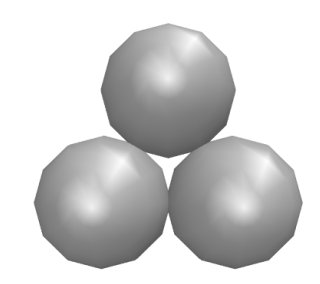
\includegraphics[width=0.15\linewidth]{Figures/fe3}
%DIFDELCMD < 	%%%
\DIFdelendFL \DIFaddbeginFL 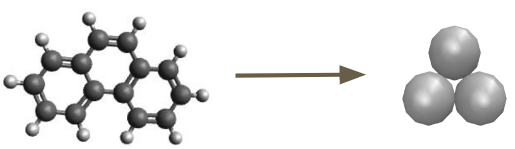
\includegraphics[width=0.70\linewidth]{Figures/fe3cg}
	\DIFaddendFL \caption{Representation of phenanthrene with the geometry proposed by \citeonline{lafitte2012}.}
	\label{fig:fen3}
\end{figure}

The first part of the estimation followed the same procedure described above for the \citeonline{muller2017} equation. However, as explained in Section \ref{parsaft}, the \citeonline{lafitte2012} equation requires the estimation of correction factors $c_{\sigma}$ and $c_{\epsilon}$ (Eqs. \eqref{eqn:csigma} and \eqref{eqn:ceps}). We then estimated these parameters by using the PSO method with Eq. \eqref{eqn:fobjla}. In this equation, vapor pressures and saturated liquid densities from molecular simulations are required. We then decided to use the Gibbs Ensemble Monte Carlo method on the NVT ensemble, explained in Section \ref{gemc}, to obtain these equilibrium properties at eight different temperatures\DIFdelbegin \DIFdel{since this method does not use an explicit interface}\DIFdelend .

The boxes for the GEMC-NVT simulations were generated by inserting 400 molecules of phenanthrene into one liquid box and 100 molecules of phenanthrene into one vapor box using the Playmol package \cite{playmol}, which is integrated with the Packmol package \cite{packmol}. Initial densities of each box were made equal to the saturated densities found with the SAFT-VR Mie Eos, aiming at avoiding the migration of all molecules to a single phase during the simulation. The GEMC-NVT simulations were executed using the Cassandra software \cite{doi:10.1063/1.3644939},  which was developed to perform Monte Carlo simulations. The equilibration and production times lasted around  $10^{4}$ and $5 \times 10^{4}$ MC cycles, respectively. Each MC cycle corresponded to $10^3$ rotation trials, $10^3$ translation trials, $10^2$ molecule insertion trials, $10^2$ molecule deletion trials, and 10 volume exchange trials. The cut-off distance was equal to $20$ \AA  $\,$ and we did not use long-range interactions. The saturated vapor density ($\rho_{vap}$), the saturated liquid density ($\rho_{liq}$), and the vapor pressure ($P_{v}$) were sampled at each 100 MC cycles. Later on, these data were divided into five blocks for calculation of their averages and standard deviations. With the correction factors found after the estimation with the simulation data, we calculated, with Eqs. \eqref{eqn:simsigma} and \eqref{eqn:simeps}, the $\sigma$ and $\epsilon$ parameters. \citeonline{lafitte2012} proposes that these are the final parameters to be used in molecular simulations. Hence, an iterative simulation is not required\DIFaddbegin \DIFadd{, }\DIFaddend and the set of optimal parameters can be obtained with one group of molecular simulations. 

\section{Solvation Free Energy Simulations}\label{solvme}

Using the parameters for phenanthrene estimated with the \citeonline{muller2017} approach and the SAFT-$\gamma$ Mie force field parameters available for other compounds, we carried out molecular dynamics simulations to estimate the solvation free energies. The chosen software package to perform the simulations was LAMMPS  \cite{lammps}. In this package, the equations of motion were integrated with the velocity-Verlet algorithm \cite{verlet} with a time step of 2 fs. As required by the coarse-grained model,  molecules with more than one bead were treated as rigid bodies. The thermostat and the barostat were the Nos\'{e}-Hoover chains as described in \citeonline{PhysRevA.31.1695}, \citeonline{doi:10.1063/1.463940}, and \citeonline{doi:10.1063/1.467468} with damping factors of 100 and 1000 time steps, respectively. For the rigid bodies in our simulations, we used the rigid-body algorithm of \citeonline{kamberaj}. Electrostatics interactions are not explicitly accounted for by the SAFT-$\gamma$ Mie force field. Hence, we did not compute Coulombic interactions. The potential cutoff was equal to 20 \AA $\,$ \cite{muller2017} with a neighbor list skin of 2 \AA. The initial configurations of the solvated systems were also generated using the Playmol package, which is integrated with the Packmol package. For the binary mixtures, one molecule of solute and a varying number of solvent molecules- 700 molecules of toluene, 700 molecules of octanol, 1024 molecules of hexane, 3000 molecules of water - were randomly added to a cubic box. Besides the systems with pure substances acting as solvents, we performed simulations to study the solvation free energy of phenanthrene in a mixture of toluene and carbon dioxide with different weight fractions ($w_{CO_{2}}$). The  system consisted of one molecule of phenanthrene for all the cases and 123 molecules of $CO_{2}$ and 618 molecules of toluene ($w_{CO_{2}} = 0.087$); 166 molecules of $CO_{2}$ and 589 molecules of toluene ($w_{CO_{2}} = 0.119$); 232 molecules of $CO_{2}$ and 545 molecules of toluene ($w_{CO_{2}} = 0.169)$; 380 molecules of $CO_{2}$ and 446 molecules of toluene ($w_{CO_{2}} = 0.289$). These substances used in our study were selected with the intention of testing the force field with standard sets used as a benchmark in solvation free energy calculations, with aromatic substances used as models to asphaltenes and with water, which probably is the most used solvent in computational studies \DIFaddbegin \DIFadd{of solvation free energies}\DIFaddend .

All simulations were performed with the constant temperature and pressure values of 298 K and 1 bar, except the ones containing carbon dioxide. These had the temperature of 298 K and the pressure of the experimental liquid-phase equilibrium corresponding to each composition of the system $CO_{2}+$toluene \cite{co2toliq}. For all simulations, the initial box was equilibrated at the NPT ensemble for 2 ns, and the resulting configurations were used as the initial configuration of the expanded ensemble simulations. These were carried out with the LAMMPS user package for expanded ensemble simulations with the Mie potential developed by our research group, available at https://github.com/atoms-ufrj/USER-ALCHEMICAL. 

During these expanded ensemble simulations, the sampling of a new alchemical state was tried at every 10 MD steps. To define the optimal values of $\lambda$ and $\eta$ corresponding to each state, trial simulations, having around 9 ns of production time, were carried out. In the first simulation, we chose the group of $\lambda$ values arbitrarily, and we either set all $\eta 's$ to zero or assigned values previously found for similar solute-solvent pairs. The subsequent group of $\eta 's$ were estimated with the flat histogram approach (Eq. \eqref{eqn:weight}). We then performed another trial simulation with the new weights. The results of this simulation were used to optimize the group of $\lambda 's$ by minimizing the number of round trips, as described in Section \ref{ee}. The $\eta 's$ corresponding to the newest group of $\lambda 's$ were interpolated linearly from the free energy differences. With the final values of $\eta$ and $\lambda $ defined for each mixture, larger simulations with a production time of 20 ns were carried out. 

Since the employed force field considers that the beads do not have charges, there are no Coulombic interactions and the $\Delta G$ in Eq. \eqref{eq:freesolv} becomes equal to $\Delta G_{3 \rightarrow 4} $. The post-processing method used to effectively calculate free energy differences with the potential energies obtained from the expanded ensemble simulations was the Multistate Bennett Acceptance Ratio (MBAR) method, described in Section \ref{mbar}. The software alchemical-analysis \cite{klimovich} was utilized to obtain the $\Delta G_{solv}$ with MBAR and to assess the quality of the results. After the first estimations, we realized that the binary interaction parameter of Eq. \eqref{eqn:epsmix} was necessary for systems containing water. Hence, we estimated  $k_{ij}$ for these pairs and, for all the other pairs, we set  $k_{ij}$ to zero. The estimation was done by performing trial expanded ensemble simulations in three values of $k_{ij}$, as suggested by \citeonline{ervik20162}. With the $\Delta G_{solv}$ obtained with these simulations, we did a linear fit to obtain the refined value of the parameter. We used this strategy because the estimation with SAFT-VR Mie EoS gave poor results for the hydration free energies.


\chapter{Results and Discussion} % Main chapter title

\label{Chapter5} % Change X to a consecutive number; for referencing this chapter elsewhere, use \ref{ChapterX}

\DIFdelbegin %DIFDELCMD < \section{Solvation free energies}
%DIFDELCMD < %%%
\DIFdelend \DIFaddbegin \section{Phenanthrene parameterization}
\DIFaddend 

The first part of this work consisted \DIFdelbegin \DIFdel{of }\DIFdelend \DIFaddbegin \DIFadd{in }\DIFaddend obtaining phenanthrene parameters for the SAFT-$\gamma$ Mie Force Field as described in Section \ref{parame}. This part was necessary since these parameters were not available for the ring geometry on the force field database \cite{ervik2016}. \DIFaddbegin \DIFadd{We carried out this parameterization using the free energy of Helmholtz equations for rings of \mbox{%DIFAUXCMD
\cite{lafitte2012}}%DIFAUXCMD
, Eq. \ref{eqn:aringlafitte}, and of \mbox{%DIFAUXCMD
\cite{muller2017}}%DIFAUXCMD
, Eq. \ref{eqn:aringmuller}. }\DIFaddend The parameters obtained \DIFaddbegin \DIFadd{with these two strategies }\DIFaddend and the mean percentage error (MPE) to the experimental data \DIFdelbegin \DIFdel{\mbox{%DIFAUXCMD
\cite{pvphen} }%DIFAUXCMD
of the vapor pressure found with the SAFT-VR Mie EoS  }\DIFdelend \DIFaddbegin \DIFadd{\mbox{%DIFAUXCMD
\cite{pvphen,osborn} }%DIFAUXCMD
}\DIFaddend were those observed in Table \ref{tbl:estimparameters}.

\begin{table}[h]
	\centering
	\caption{Estimated SAFT-$\gamma$ Mie force field parameters for phenanthrene.}
	\label{tbl:estimparameters}
	\begin{tabular}{ccccc}
		\hline\hline
		$m_s$                & $\epsilon/\kappa_{b}$ (K) & $\sigma$ (\AA) & $\lambda_r$ & MPE(\%)   \\ \hline\hline
		3 \cite{lafitte2012} & 485.55               & 4.197              & 14.34       & 1.48|9.74 \\
		5  \cite{muller2017} & 262.74               & 4.077              & 9.55        & 0.88      \\ \hline\hline
	\end{tabular}

\end{table} 

The MPE value of 1.64 for the \citeonline{lafitte2012} strategy in the Table \ref{tbl:estimparameters} is the error between the vapor pressure calculated with the equation of state and the experimental data. The second MPE value for the \citeonline{lafitte2012} strategy (9.74) is the error between the vapor pressure calculated with the equation of state and the vapor pressure obtained in the GEMC simulations. \DIFdelbegin \DIFdel{The \mbox{%DIFAUXCMD
\citeonline{lafitte2012}  }%DIFAUXCMD
strategy should not need }\DIFdelend \DIFaddbegin \DIFadd{We also show, in Figure \ref{fig:fitede}, the vapor pressure curve obtained using the EoS with the two free energy of Helmholtz equations for rings. It's clear, observing the figure mentioned above and the MPE     values for both equations for rings, that both approaches for the EoS performed very similar and were able to reproduce the experimental data. However, the parameters estimated with the equation of \mbox{%DIFAUXCMD
\citeonline{lafitte2012}  }%DIFAUXCMD
could not be directly transferred to molecular simulations because this strategy needs }\DIFaddend an estimation with molecular simulation\DIFdelbegin \DIFdel{data since this }\DIFdelend \DIFaddbegin \DIFadd{. This }\DIFaddend additional procedure is not necessary when estimating parameters for the chain equation \cite{avendano2011} or the ring equation of \citeonline{muller2017}. In addition to that, this use of molecular simulation data to acquire the parameters negates the overall idea proposed by \cite{avendano2011}. They developed this force field with the intention of obtaining the parameters in a more straightforward way than other force fields since the SAFT-$\gamma$ Mie model would not have the computational time associated with doing molecular simulations in its parameterization. Due to these specific characteristics of the model of \citeonline{lafitte2012}, we only studied the solvation free energy of phenanthrene with the set of parameters estimated with the strategy of \citeonline{muller2017}. In fact, we only followed the \DIFdelbegin \DIFdel{strategy }\DIFdelend \DIFaddbegin \DIFadd{approach }\DIFaddend of \citeonline{lafitte2012} because it was the only one available when we first started this research. The sets of parameters \DIFaddbegin \DIFadd{and geometries }\DIFaddend for the other compounds were retrieved from the literature\DIFdelbegin \DIFdel{\mbox{%DIFAUXCMD
\cite{lobanova2016,herdes2015,ervik2016,muller2017}}%DIFAUXCMD
, and all the utilized parameters are available in Table \ref{tbl:parameters} }\DIFdelend \DIFaddbegin \DIFadd{, and they are exposed in Tables \ref{tbl:parameters} and \ref{tbl:geopara}}\DIFaddend .

\DIFdelbegin %DIFDELCMD < \begin{table}[h]
%DIFDELCMD < 	%%%
\DIFdelendFL \DIFaddbeginFL \begin{figure}[h]
	\DIFaddendFL \centering
	\DIFaddbeginFL 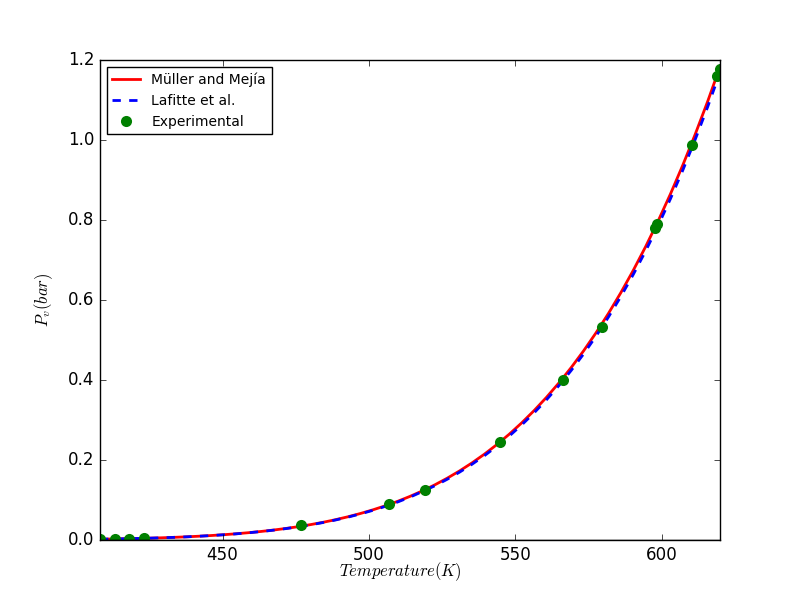
\includegraphics[width=0.8\linewidth]{Figures/ede}
	\DIFaddendFL \caption{\DIFdelbeginFL \DIFdelFL{Parameters }\DIFdelendFL \DIFaddbeginFL \DIFaddFL{Vapor pressure ($P_{v}$) calculated with the two strategies }\DIFaddendFL of the \DIFdelbeginFL \DIFdelFL{SAFT-$\gamma$ }\DIFdelendFL \DIFaddbeginFL \DIFaddFL{SAFT-VR }\DIFaddendFL Mie \DIFdelbeginFL \DIFdelFL{force field }\DIFdelendFL \DIFaddbeginFL \DIFaddFL{EoS }\DIFaddendFL for \DIFdelbeginFL \DIFdelFL{each substance used in this work}\DIFdelendFL \DIFaddbeginFL \DIFaddFL{modeling molecules formed by rings}\DIFaddendFL .} 
	\DIFdelbeginFL %DIFDELCMD < %DIFDELCMD < \label{tbl:parameters}%%%
%DIFDELCMD < 	\begin{tabular}{ccccc}
%DIFDELCMD < 		\hline
%DIFDELCMD < 		\hline
%DIFDELCMD < 		& %%%
\DIFdelFL{$m_s$ }%DIFDELCMD < & %%%
\DIFdelFL{$\epsilon/\kappa_{b}$ (K) }%DIFDELCMD < & %%%
\DIFdelFL{$\sigma$ (\AA) }%DIFDELCMD < & %%%
\DIFdelFL{$\lambda_r$ }%DIFDELCMD < \\ \hline\hline
%DIFDELCMD < 		%%%
\DIFdelFL{Water          }%DIFDELCMD < & %%%
\DIFdelFL{1     }%DIFDELCMD < & %%%
\DIFdelFL{305.21               }%DIFDELCMD < & %%%
\DIFdelFL{2.902              }%DIFDELCMD < & %%%
\DIFdelFL{8.0         }%DIFDELCMD < \\
%DIFDELCMD < 		%%%
\DIFdelFL{Propane        }%DIFDELCMD < & %%%
\DIFdelFL{1     }%DIFDELCMD < & %%%
\DIFdelFL{426.08               }%DIFDELCMD < & %%%
\DIFdelFL{4.871              }%DIFDELCMD < & %%%
\DIFdelFL{34.29       }%DIFDELCMD < \\
%DIFDELCMD < 		%%%
\DIFdelFL{Carbon dioxide }%DIFDELCMD < & %%%
\DIFdelFL{2     }%DIFDELCMD < & %%%
\DIFdelFL{194.94               }%DIFDELCMD < & %%%
\DIFdelFL{2.848              }%DIFDELCMD < & %%%
\DIFdelFL{14.65       }%DIFDELCMD < \\
%DIFDELCMD < 		%%%
\DIFdelFL{Hexane         }%DIFDELCMD < & %%%
\DIFdelFL{2     }%DIFDELCMD < & %%%
\DIFdelFL{376.35               }%DIFDELCMD < & %%%
\DIFdelFL{4.508              }%DIFDELCMD < & %%%
\DIFdelFL{19.57       }%DIFDELCMD < \\
%DIFDELCMD < 		%%%
\DIFdelFL{Octanol        }%DIFDELCMD < & %%%
\DIFdelFL{3     }%DIFDELCMD < & %%%
\DIFdelFL{495.71               }%DIFDELCMD < & %%%
\DIFdelFL{4.341              }%DIFDELCMD < & %%%
\DIFdelFL{28.79       }%DIFDELCMD < \\
%DIFDELCMD < 		%%%
\DIFdelFL{Toluene        }%DIFDELCMD < & %%%
\DIFdelFL{3     }%DIFDELCMD < & %%%
\DIFdelFL{268.24               }%DIFDELCMD < & %%%
\DIFdelFL{3.685              }%DIFDELCMD < & %%%
\DIFdelFL{11.80       }%DIFDELCMD < \\
%DIFDELCMD < 		%%%
\DIFdelFL{Benzene        }%DIFDELCMD < & %%%
\DIFdelFL{3     }%DIFDELCMD < & %%%
\DIFdelFL{230.30               }%DIFDELCMD < & %%%
\DIFdelFL{3.441              }%DIFDELCMD < & %%%
\DIFdelFL{10.45       }%DIFDELCMD < \\
%DIFDELCMD < 		%%%
\DIFdelFL{Pyrene         }%DIFDELCMD < & %%%
\DIFdelFL{4     }%DIFDELCMD < & %%%
\DIFdelFL{459.04               }%DIFDELCMD < & %%%
\DIFdelFL{4.134              }%DIFDELCMD < & %%%
\DIFdelFL{15.79       }%DIFDELCMD < \\
%DIFDELCMD < 		%%%
\DIFdelFL{Anthracene     }%DIFDELCMD < & %%%
\DIFdelFL{5     }%DIFDELCMD < & %%%
\DIFdelFL{259.68               }%DIFDELCMD < & %%%
\DIFdelFL{3.631              }%DIFDELCMD < & %%%
\DIFdelFL{9.55        }%DIFDELCMD < \\ 
%DIFDELCMD < 		\hline
%DIFDELCMD < 		\hline
%DIFDELCMD < 	\end{tabular}
%DIFDELCMD < 	%%%
\DIFdelendFL \DIFaddbeginFL \label{fig:fitede}
\end{figure}
\DIFaddendFL 

\DIFdelbeginFL %DIFDELCMD < \end{table}
%DIFDELCMD < \FloatBarrier
%DIFDELCMD < %%%
\DIFdelend \DIFaddbegin \section{Solvation free energies}
\DIFaddend Our primary intention with this study is to assess the capability of the SAFT-$\gamma$ Mie force field to represent solvation free energies. Hence, we chose benchmark solutes used in the literature (benzene, propane) and polyaromatic solutes (benzene, pyrene, phenanthrene, anthracene), and, for the solvents, we picked non-polar (hexane), aromatic (toluene), and hydrogen bonding (1-octanol, water) substances. It would be interesting to do a study with a bigger database of pairs solvent-solute. However, the time required for performing each of the solvation free energy simulations, some difficulties related to the available computational structure, and the fact that a better model of aromatic compounds with this force field was only published in the middle of our study prevented us from doing a more extensive study. The solvation free energy simulations for the pairs chosen were carried out with binary interaction parameters equal to zero since these parameters were not necessary according to our preliminary studies. Since the force field does not account for charges, we only calculated the Mie contribution (Eq. \eqref{eq:softcore}) to the solvation free energy. A total of 15 to 18 $\lambda 's$, depending on the solute-solvent pairs, and their respective $\eta 's$ were estimated as described in Sections \ref{ee} and \ref{solvme}. The \DIFaddbegin \DIFadd{simulations carried out using these optimized weights deviated from the flat-histogram requirement of equal number visits by an average of 5\% for all of the pairs solvent+solute. The }\DIFaddend final $\lambda$ set for all the pairs was found using the cumulative probability distribution (Eq. \eqref{eqn:cumfun}). The probability distribution for the hexane(solvent)+benzene(solute) pair can be seen in \figref{fig:optimized_cdf}. From now on we are going to use the terminology solvent+solute. The optimized values of $\lambda$ and $\eta$ for this pair and all the other pairs are available in Tables \ref{tbl:lambdahex} to \ref{tbl:lambdaco2}. By observing the coupling parameters found for all the pairs, we can see that they are concentrated on the region with a steeper slope as it is expected in this method.
\DIFdelbegin %DIFDELCMD < \FloatBarrier
%DIFDELCMD < %%%
\DIFdelend \DIFaddbegin 

\DIFaddend \begin{figure}[h]
	\centering
	\DIFdelbeginFL %DIFDELCMD < 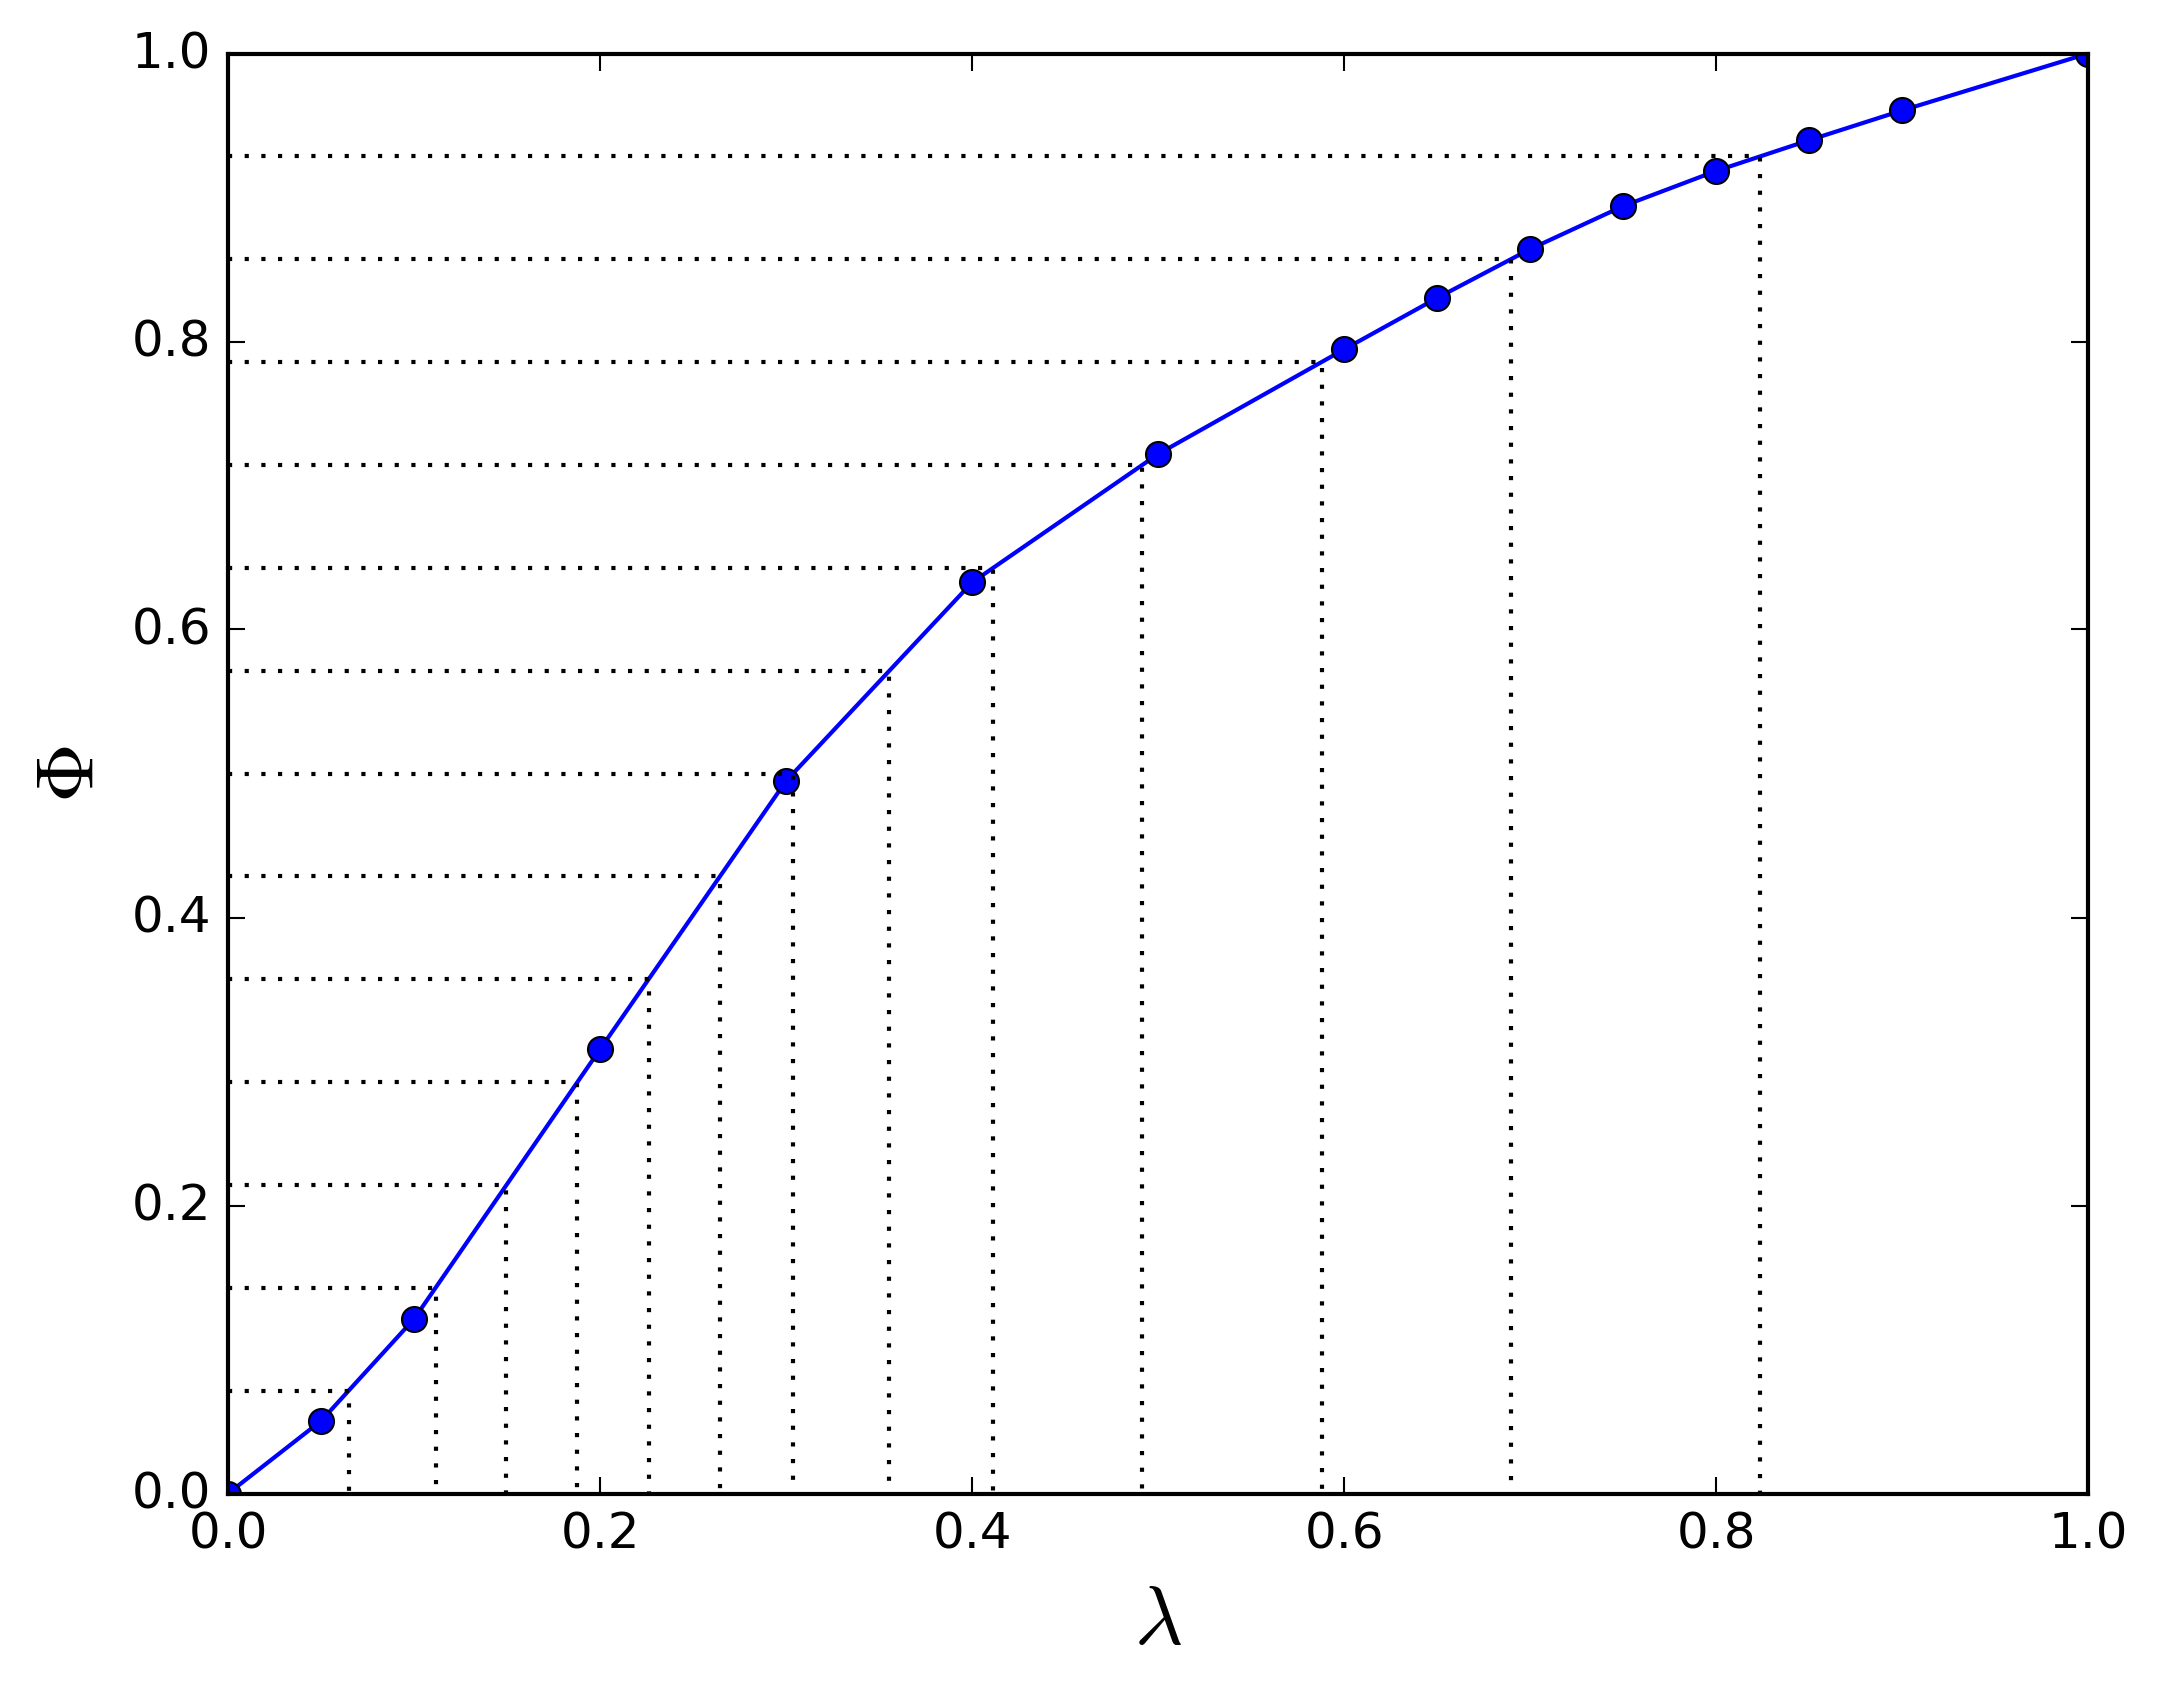
\includegraphics[width=0.8\linewidth]{Figures/optimized_cdf}
%DIFDELCMD < 	%%%
\DIFdelendFL \DIFaddbeginFL 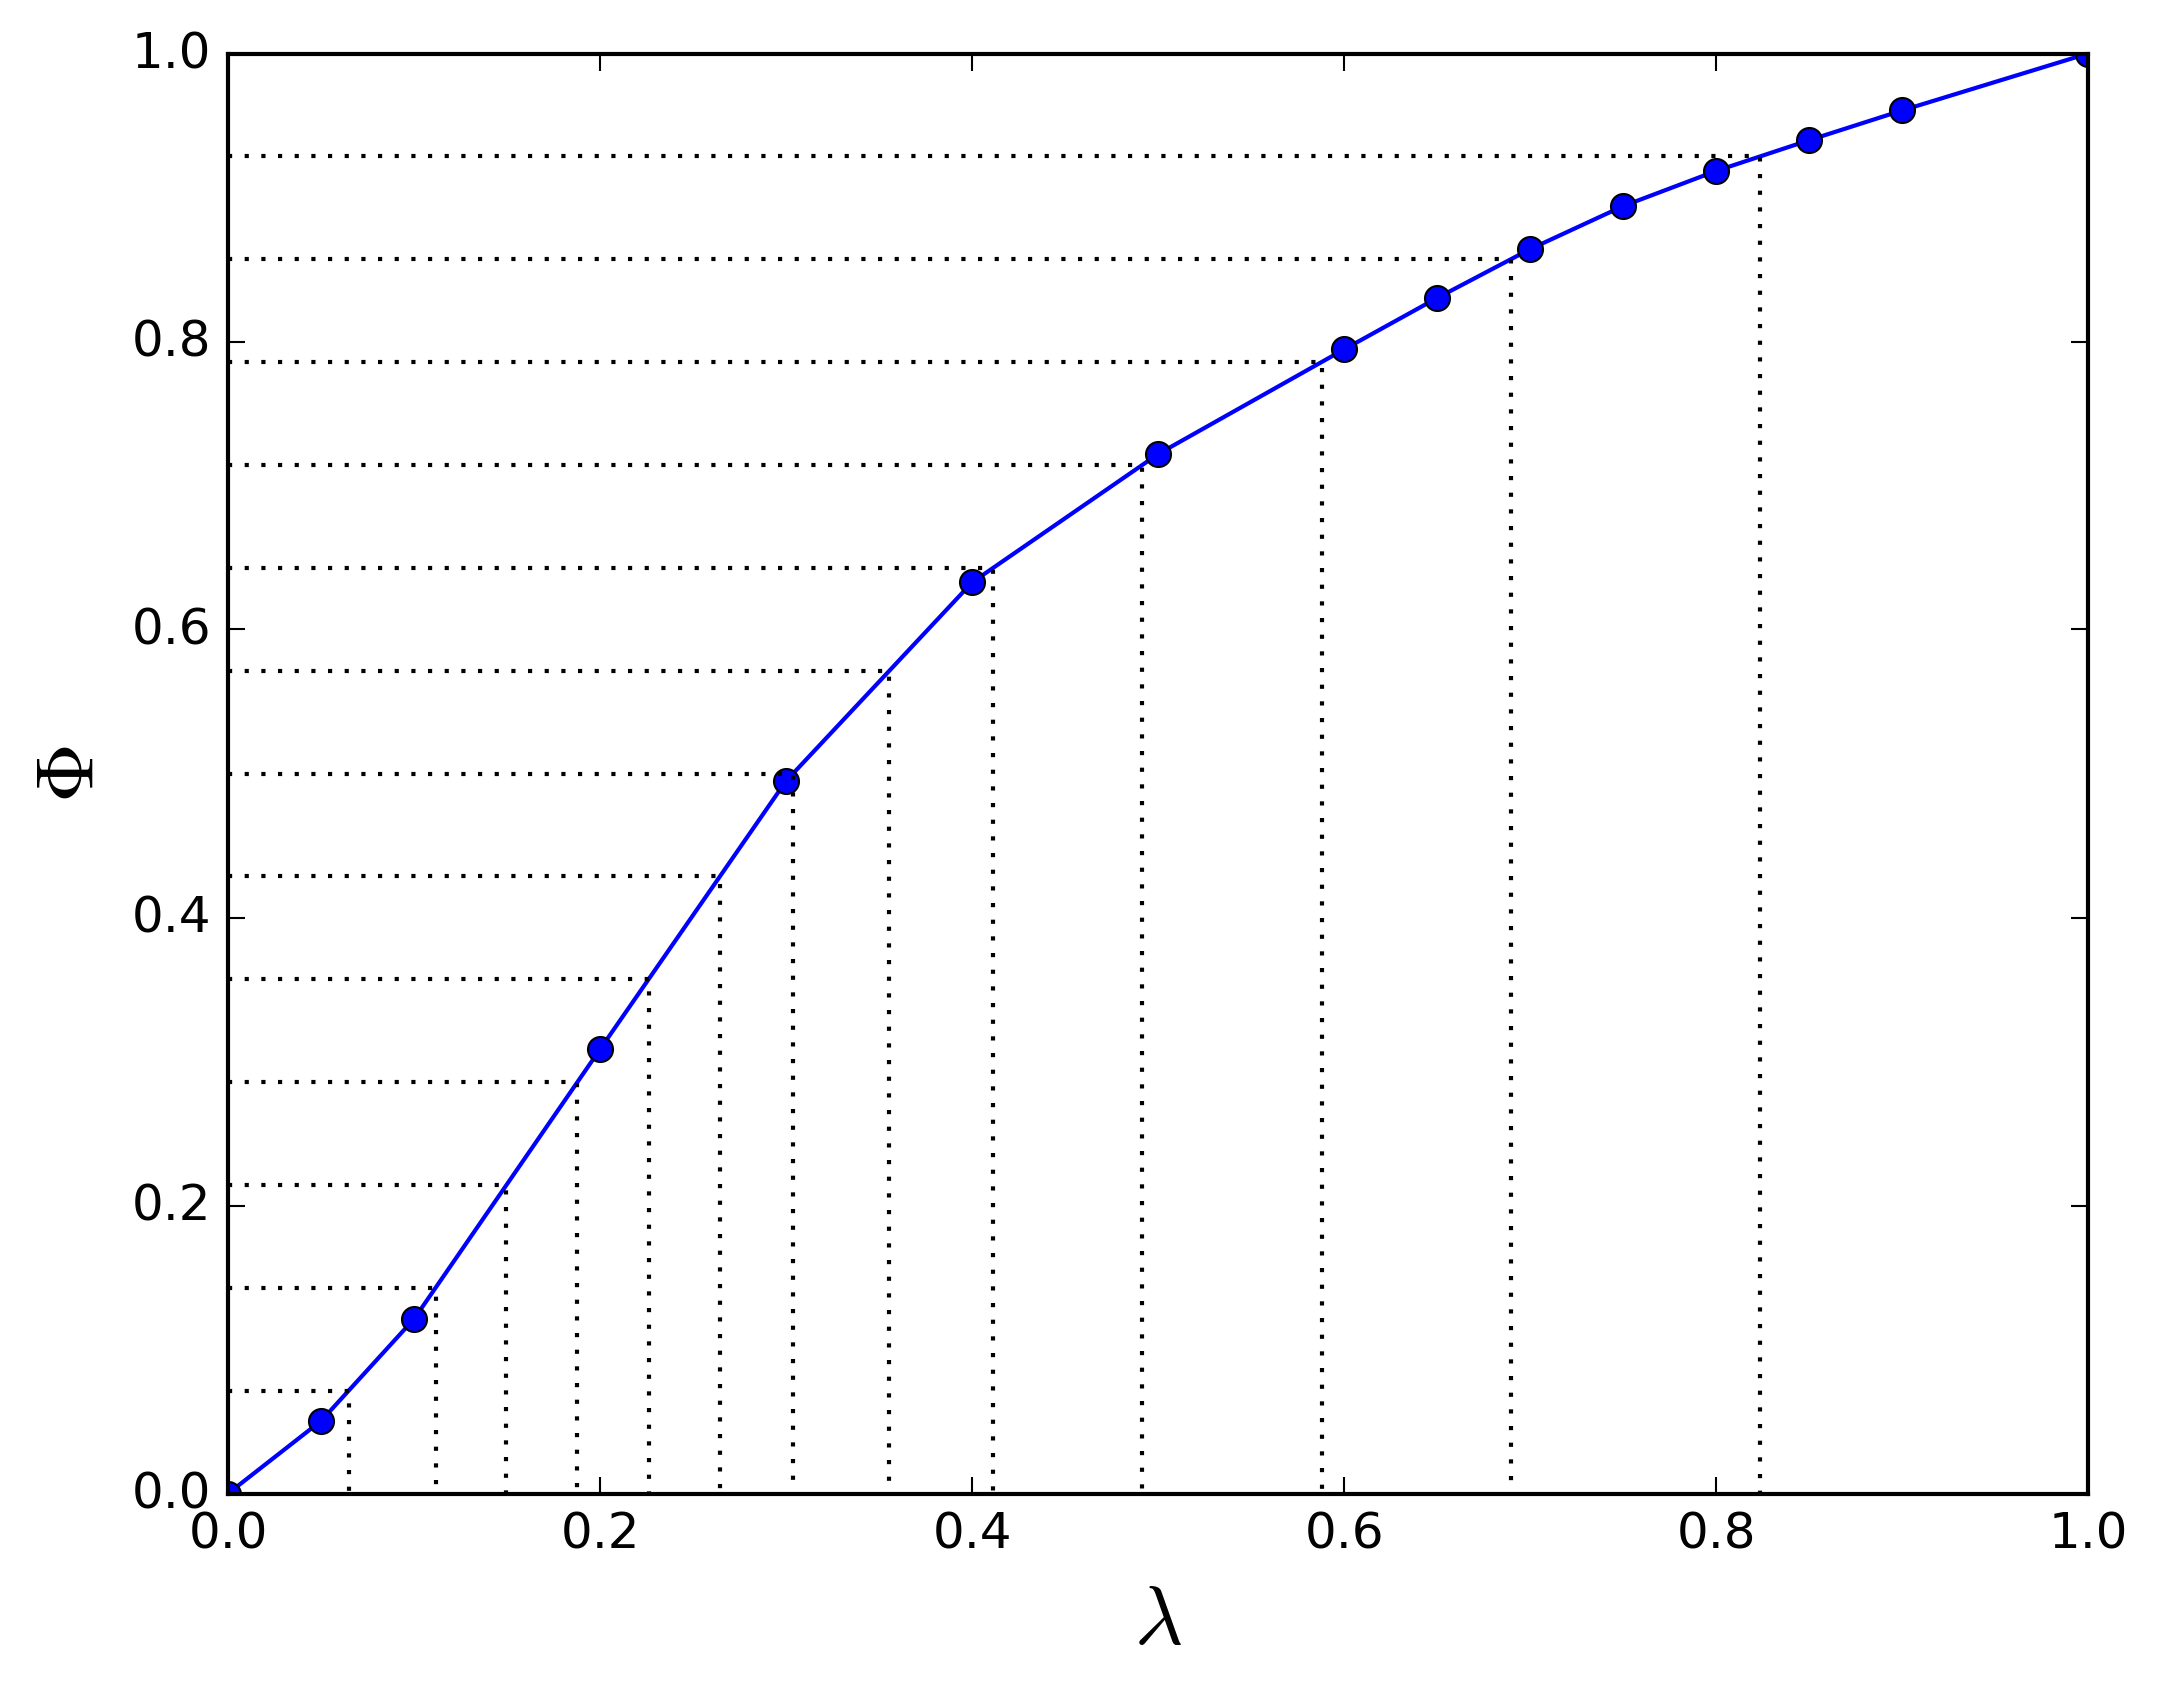
\includegraphics[width=0.72\linewidth]{Figures/optimized_cdf}
	\DIFaddendFL \caption{Cumulative probability used to obtain the optimized values of $\lambda 's$ for the pair hexane+benzene.}
	\label{fig:optimized_cdf}
\end{figure}

%DIF > Simulations using these weights deviated
%DIF > by an average of 5% from flat histogram occupancy
%DIF > in states, with an average maximum deviation over all
%DIF > simulations of less than 10%.
\DIFaddbegin 

\DIFaddend \begin{table}[h]
	\centering
	\caption{Optimized values of $\lambda $ and $\eta $ for the hexane+solute pairs.}
	\label{tbl:lambdahex}
	\begin{tabular}{cccccc}
		\hline\hline
		\multicolumn{2}{c}{benzene}&\multicolumn{2}{c}{pyrene}& \multicolumn{2}{c}{phenanthrene}\\
		\hline\hline
		$\lambda$ & $\eta$& $\lambda$ & $\eta$  & $\lambda$ & $\eta$   \\ 
		\hline\hline
		0.000     &0.000      & 0.000    &    0.000    &    0.000    &    0.000    \\
		0.065     &0.708  & 0.076    &    4.234    &    0.090    &    1.981    \\
		0.112     &1.385  & 0.107    &    5.620    &    0.132    &    3.461    \\
		0.15      &1.892  & 0.132    &    6.499    &    0.161    &    4.494    \\
		0.188     &2.399  & 0.152    &    6.690    &    0.185    &    5.185    \\
		0.226     &2.519  & 0.170    &    6.643    &    0.205    &    5.552    \\
		0.264     &2.457  & 0.189    &    6.461    &    0.224    &    5.725    \\
		0.304     &2.367  & 0.213    &    6.091    &    0.244    &    5.722    \\
		0.356     &1.921  & 0.242    &    5.566    &    0.268    &    5.523    \\
		0.411     &1.411  & 0.280    &    4.729    &    0.305    &    4.975    \\
		0.492     &0.524  & 0.355    &    2.853    &    0.372    &    3.576    \\
		0.588     &-0.663 & 0.483    &    -0.778    &    0.500    &    0.297    \\
		0.69      &-2.016 & 0.678    &    -6.947    &    0.560    &    -1.390    \\
		0.824     &-3.922 & 0.788    &    -10.631    &    0.722    &    -6.309    \\
		1.000         &-6.583  &1.000      &    -18.141    &    1.000    &    -15.448    \\
		\hline\hline   
	\end{tabular}
\end{table}
\begin{table}[h]
	\centering
	\caption{Optimized values of $\lambda $ and $\eta$ for the 1-octanol+solute pairs.}
	\begin{tabular}{cccccc}
		\hline\hline
		\multicolumn{2}{c}{propane}& \multicolumn{2}{c}{anthracene}& \multicolumn{2}{c}{phenanthrene}\\
		\hline\hline
		$\lambda$ & $\eta$ & $\lambda$ & $\eta$  & $\lambda$ & $\eta$   \\ 
		\hline\hline
		0.000    &    0.000    &    0.000    &    0.000    &    0.000    &    0.000    \\
		0.027    &    3.126    &    0.078    &    3.932    &    0.049    &    2.578    \\
		0.050    &    5.109    &    0.111    &    6.178    &    0.091    &    5.663    \\
		0.073    &    6.093    &    0.130    &    7.426    &    0.125    &    8.575    \\
		0.095    &    6.570    &    0.143    &    8.201    &    0.144    &    10.069    \\
		0.117    &    6.826    &    0.154    &    8.717    &    0.157    &    10.978    \\
		0.142    &    6.956    &    0.164    &    9.085    &    0.169    &    11.599    \\
		0.174    &    6.969    &    0.174    &    9.357    &    0.180    &    12.040    \\
		0.215    &    6.847    &    0.184    &    9.556    &    0.192    &    12.340    \\
		0.269    &    6.554    &    0.197    &    9.676    &    0.206    &    12.499    \\
		0.337    &    6.050    &    0.214    &    9.681    &    0.225    &    12.478    \\
		0.427    &    5.228    &    0.238    &    9.490    &    0.253    &    12.161    \\
		0.545    &    3.955    &    0.274    &    8.958    &    0.298    &    11.280    \\
		0.720    &    1.843    &    0.326    &    7.906    &    0.371    &    9.406    \\
		1.000    &    -1.903    &    0.399    &    6.088    &    0.484    &    5.891    \\
		&        &    0.515    &    2.777    &    0.664    &    -0.516    \\
		&        &    0.695    &    -2.960    &    0.802    &    -5.908    \\
		&        &    1.000    &    -13.768    &    1.000    &    -14.073    \\
		\hline\hline
	\end{tabular}
\end{table}
\begin{table}[h]
	\centering
	\caption{Optimized values of $\lambda $ and $\eta$ for the toluene+solute pairs.}
	\begin{tabular}{cccccc}
		\hline\hline
		\multicolumn{2}{c}{pyrene}& \multicolumn{2}{c}{anthracene}& \multicolumn{2}{c}{phenanthrene}\\
		\hline\hline
		$\lambda$ & $\eta$ & $\lambda$ & $\eta$  & $\lambda$ & $\eta$   \\ 
		\hline\hline
		0.000    &    0.000    &    0.000    &    0.000    &    0.000    &    0.000    \\
		0.090    &    2.563    &    0.119    &    0.218    &    0.136    &    0.726    \\
		0.130    &    4.338    &    0.174    &    1.210    &    0.191    &    2.307    \\
		0.154    &    5.439    &    0.209    &    2.052    &    0.223    &    3.430    \\
		0.172    &    6.181    &    0.236    &    2.664    &    0.246    &    4.233    \\
		0.188    &    6.670    &    0.261    &    3.122    &    0.264    &    4.780    \\
		0.204    &    6.986    &    0.283    &    3.378    &    0.281    &    5.149    \\
		0.222    &    7.121    &    0.306    &    3.449    &    0.299    &    5.354    \\
		0.244    &    7.025    &    0.332    &    3.311    &    0.318    &    5.389    \\
		0.278    &    6.520    &    0.360    &    2.936    &    0.340    &    5.222    \\
		0.340    &    5.010    &    0.399    &    2.209    &    0.372    &    4.717    \\
		0.462    &    1.247    &    0.466    &    0.567    &    0.425    &    3.440    \\
		0.616    &    -4.283    &    0.564    &    -2.211    &    0.524    &    0.444    \\
		0.788    &    -11.032    &    0.715    &    -6.983    &    0.701    &    -5.814    \\
		1.000    &    -19.814    &    1.000    &    -16.923    &    1.000    &    -17.803    \\        
		\hline\hline
	\end{tabular}
\end{table}
\DIFdelbegin %DIFDELCMD < \FloatBarrier
%DIFDELCMD < %%%
\DIFdelend \DIFaddbegin 

\DIFaddend \begin{table}[h]
	\centering
	\caption{Optimized values of $\lambda $ and $\eta $ for the phenanthrene+$CO_{2}$+ toluene mixture with different values of $w_{CO_{2}}$.}
	\label{tbl:lambdaco2}
	\begin{tabular}{cccccccc}
		\hline\hline
		\multicolumn{2}{c}{$w_{CO_{2}}=0.087$}& \multicolumn{2}{c}{$w_{CO_{2}}=0.119$}& \multicolumn{2}{c}{$w_{CO_{2}}=0.169$}& \multicolumn{2}{c}{$w_{CO_{2}}=0.289$}\\
		\hline\hline
		$\lambda$ & $\eta$ & $\lambda$ & $\eta$  & $\lambda$ & $\eta$  & $\lambda$ & $\eta$ \\ 
		\hline\hline
		0.000    &    0.000    &    0.000    &    0.000    &    0.000    &    0.000    &    0.000    &    0.000    \\
		0.128    &    0.604    &    0.128    &    0.732    &    0.064    &    0.883    &    0.066    &    0.806    \\
		0.184    &    2.067    &    0.186    &    2.223    &    0.108    &    0.764    &    0.111    &    0.760    \\
		0.217    &    3.164    &    0.219    &    3.319    &    0.175    &    1.969    &    0.172    &    1.983    \\
		0.240    &    3.940    &    0.244    &    4.098    &    0.214    &    3.156    &    0.204    &    2.967    \\
		0.260    &    4.472    &    0.267    &    4.704    &    0.240    &    3.974    &    0.227    &    3.627    \\
		0.277    &    4.823    &    0.289    &    5.031    &    0.258    &    4.457    &    0.245    &    4.082    \\
		0.295    &    5.035    &    0.313    &    5.084    &    0.273    &    4.750    &    0.262    &    4.395    \\
		0.318    &    5.059    &    0.339    &    4.950    &    0.287    &    4.921    &    0.279    &    4.583    \\
		0.347    &    4.762    &    0.373    &    4.371    &    0.305    &    4.962    &    0.299    &    4.621    \\
		0.397    &    3.753    &    0.425    &    3.055    &    0.326    &    4.885    &    0.325    &    4.423    \\
		0.491    &    1.031    &    0.488    &    1.196    &    0.361    &    4.401    &    0.365    &    3.739    \\
		0.670    &    -5.148    &    0.525    &    -0.027    &    0.419    &    2.990    &    0.428    &    2.198    \\
		0.791    &    -9.713    &    0.730    &    -7.185    &    0.527    &    -0.299    &    0.530    &    -0.842    \\
		1.000    &    -18.098    &    1.000    &    -17.769    &    0.697    &    -6.180    &    0.701    &    -6.763    \\
		&        &        &        &    1.000    &    -17.998    &    1.000    &    -18.163    \\
		\hline\hline
	\end{tabular}
\end{table}
\DIFdelbegin %DIFDELCMD < 

%DIFDELCMD < %%%
\DIFdelend \DIFaddbegin \FloatBarrier
\DIFaddend It is also essential to analyze the reliability of solvation free energy estimations through the overlapping of the intermediate states. Insufficient overlap among states when using FEP based methods such as MBAR may result in the underestimation of variance and, consequently, in substantially incorrect solvation free energies \cite{klimovich}. The overlap matrix for the solvation free energy of benzene in hexane is presented in \figref{fig:hexove} and the matrices for the other pairs are available in Appendix \ref{overlapmatrix}. Each element $ij$ of these matrices is the average probability of observing a configuration sampled from state i in state j. As an example, the average probability of finding a configuration sampled from state 3 in state 4 is 0.11 in \figref{fig:hexove}. According to \citeonline{klimovich}, a tridiagonal overlap matrix is an indication of reliable free energy estimates, as long as the resulting error is sufficiently low. They define a tridiagonal matrix as one matrix with elements appreciably different from zero (the values should be as low as 0.03) in the main diagonal and the first diagonals above and below the main one. This requirement was met for all the pairs in our study. Some of the overlap matrices, including the one in Figure \ref{fig:hexove}, had more than three diagonals, and, consequently, an apparent unnecessary number of intermediate states. However, this number of intermediate states was indispensable in our study because the error estimate of the solvation free energies significantly increased when we removed some of the intermediate states. Hence, we maintained these intermediate states in order to obtain low error values. After this analysis, we present in Table \ref{tbl:solv1} the results for solvation free energy calculations\DIFaddbegin \DIFadd{, the errors from these estimations with MBAR, }\DIFaddend and the absolute deviations from experimental data \cite{doi:10.1021/ci034120c}.  

\begin{figure}[h]
	\centering
	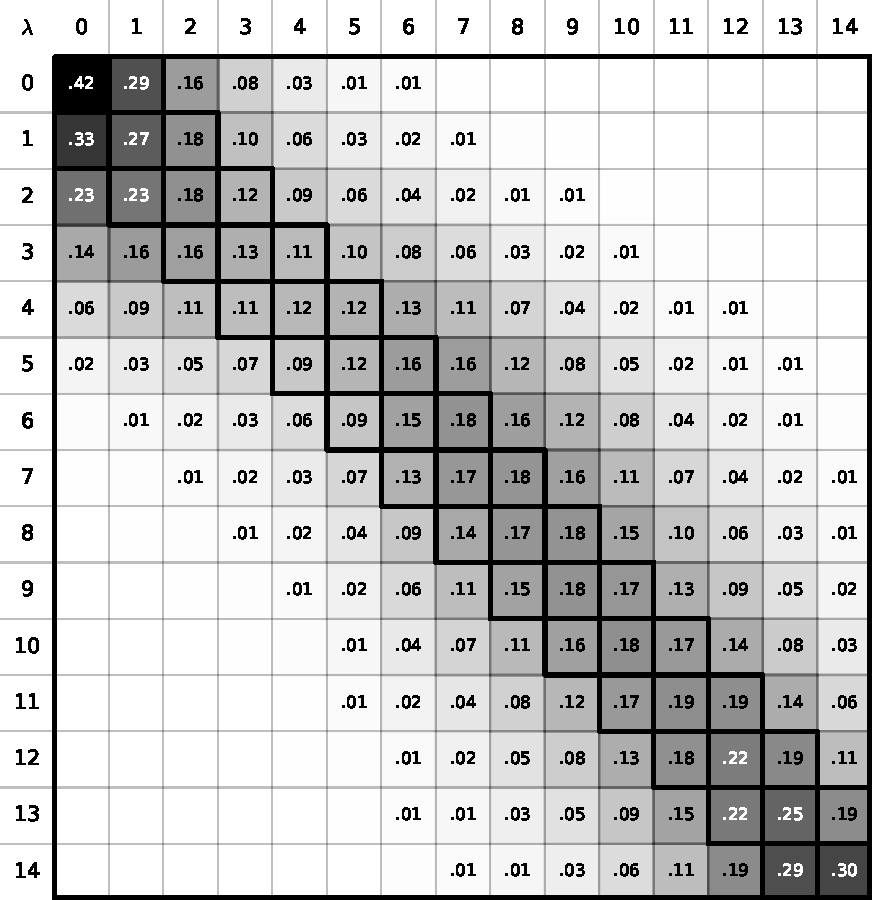
\includegraphics[width=0.7\textwidth]{Figures/ohex_benz}
	\caption{Overlap matrix for hexane+benzene.}
	\label{fig:hexove}
\end{figure}

\begin{table}[h]
	\centering
	\caption{Calculated and experimental values for the solvation free energies (kcal/mol) of solutes in non-aqueous solvents.}
	\label{tbl:solv1}
	\begin{tabular}{cccccc}
		\hline\hline
		Solute       & Solvent   & $\Delta G_{solv}^{exp}$ & $\Delta G_{solv}^{Mie}$ & Absolute  &  \\
		&           &                         &                         & Deviation &  \\ \hline\hline
		benzene      & hexane    & -3.96                   & -3.76  $\,$ $\pm$ 0.01       & 0.20      &  \\
		pyrene       & hexane    & -11.53                  & -10.82 $\pm$ 0.02       & 0.71      &  \\
		phenanthrene & hexane    & -10.01                  & -9.16  $\,$ $\pm$ 0.01       & 0.85      &  \\
		propane      & 1-octanol & -1.32                   & -1.36  $\,$ $\pm$ 0.03       & 0.04      &  \\
		anthracene   & 1-octanol & -11.72                  & -8.12   $\,$ $\pm$ 0.03       & 3.61      &  \\
		phenanthrene & 1-octanol & -10.22                  & -8.34  $\,$ $\pm$ 0.03       & 1.47      &  \\
		pyrene       & toluene   & -12.86                  & -11.74 $\pm$ 0.01       & 1.11      &  \\
		anthracene   & toluene   & -11.31                  & -9.90 $\,$ $\pm$ 0.01        & 1.41      &  \\ \hline\hline
		&
	\end{tabular}
\end{table}
\DIFaddbegin \FloatBarrier
\DIFaddend 

The numerical values for solvation free energies in hexane had overall smaller absolute deviations from experimental data than the deviations in the other solvents. Additionally, this force field presented better results for the pair hexane+benzene than the TraPPE force field (- 4.35  $\pm$ 0.05 kcal/mol) \cite{garrido2011} and the ELBA coarse-grained force field  (-2.92 $\pm$ 0.01 kcal/mol) \cite{doi:10.1021/acs.jctc.5b00963}. TraPPE is a force field parametrized with fluid-phase equilibria data that uses the Lennard-Jones potential to describe the non-bonded interactions. In the cited paper, they used the united-atom description of the TraPPE force field for the alkyl group, the all-atom description for the polar groups and the explicit-hydrogen approach for the aromatic groups. In the explicit-hydrogen approach, the interaction sites for all hydrogen atoms, some lone pair electrons, and bond centers are accounted for \cite{doi:10.1021/jp073586l}. In turn, the ELBA force field is a coarse-grained model that comprises six independent parameters. This force field models three carbons as one Lennard-Jones site and one water molecule as a single \DIFdelbegin \DIFdel{Lennard Jones }\DIFdelend \DIFaddbegin \DIFadd{Lennard-Jones }\DIFaddend site with a point dipole. We also present the solvation free energies corresponding to each alchemical state ($\lambda$) for all the pairs studied here in Figures \ref{fig:hex} to \ref{fig:tol}. \DIFaddbegin \DIFadd{In these figures, we did not represent the errors of the estimation with MBAR because they were too small to be seen. }\DIFaddend Specifically observing the solvation free energy in hexane (Figure \ref{fig:hex}), we can see the effect of the molecule's size on the entropic region of the free energy curve. This region corresponds to the first values of $\lambda$ where space in the solvent is being 'opened' for the insertion of the solute.

We expected that a force field based on an EoS that does not explicitly account for hydrogen bond would not perform well for 1-octanol in mixtures since the parameterization of this molecule did not explicitly account for the interactions of association. All the beads representing 1-octanol have the same intermolecular parameter, and there is no distinction between the polar and apolar groups. Despite this, the solvation free energies of propane and phenanthrene in 1-octanol lied in the desired deviation range of 1-2 kcal/mol \cite{doimobley}. For propane, the observed deviation in solvation free energies was much smaller when compared to the other solutes, which can be attributed to the \DIFdelbegin \DIFdel{non polarity }\DIFdelend \DIFaddbegin \DIFadd{non-polarity }\DIFaddend of propane and its smoother free energy curve, presented in Figure \ref{fig:oct}. Such solvation free energy of propane in 1-octanol also had a smaller deviation than the prediction of the ELBA force field (-0.92 $\pm$ 0.01) \cite{doi:10.1021/acs.jctc.5b00963}. The absolute deviation of the solvation free energy computed for anthracene in 1-octanol is much higher than the one calculated for phenanthrene in 1-octanol. The anthracene and phenanthrene molecules have the same geometry (Figure \ref{fig:fen5}) in the SAFT-$\gamma$ Mie model, although anthracene is a linear molecule and phenanthrene is not, and also similar physical properties. Hence, this high deviation of the solvation free energy of anthracene in 1-octanol may indicate a problem in the geometry chosen for anthracene in the SAFT-$\gamma$ Mie force field and the importance of the geometry in modeling the molecules with this force field.      
\FloatBarrier
\begin{figure}[H]
	\centering
	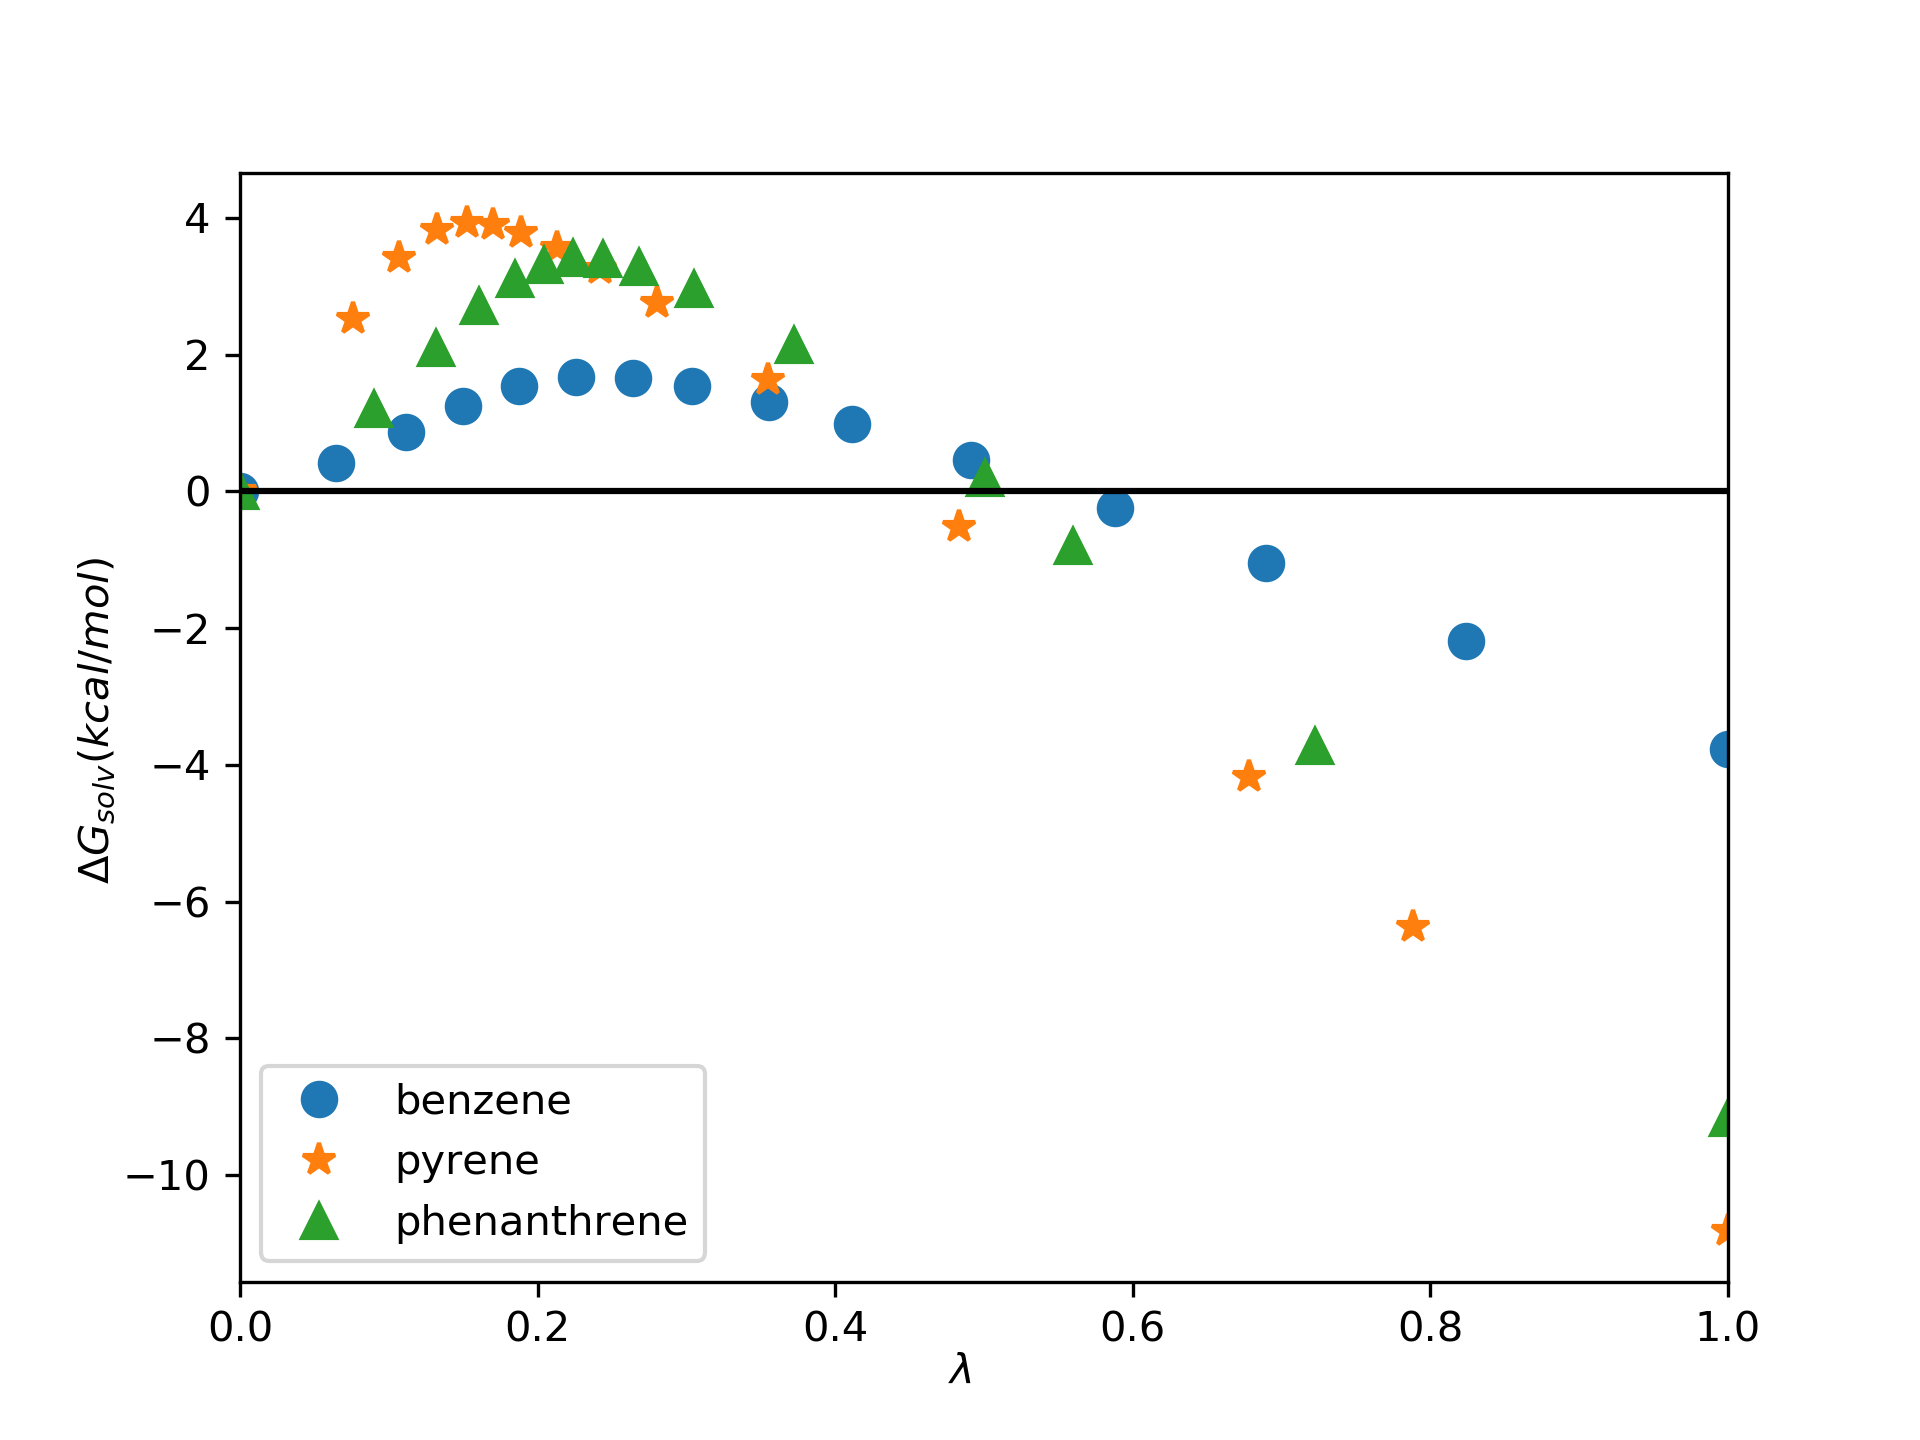
\includegraphics[width=0.8\textwidth]{Figures/hex}
	\caption{Representation of solvation free energies of different solutes in hexane corresponding to each alchemical state.}
	\label{fig:hex}
\end{figure}

\begin{figure}[H]
	\centering
	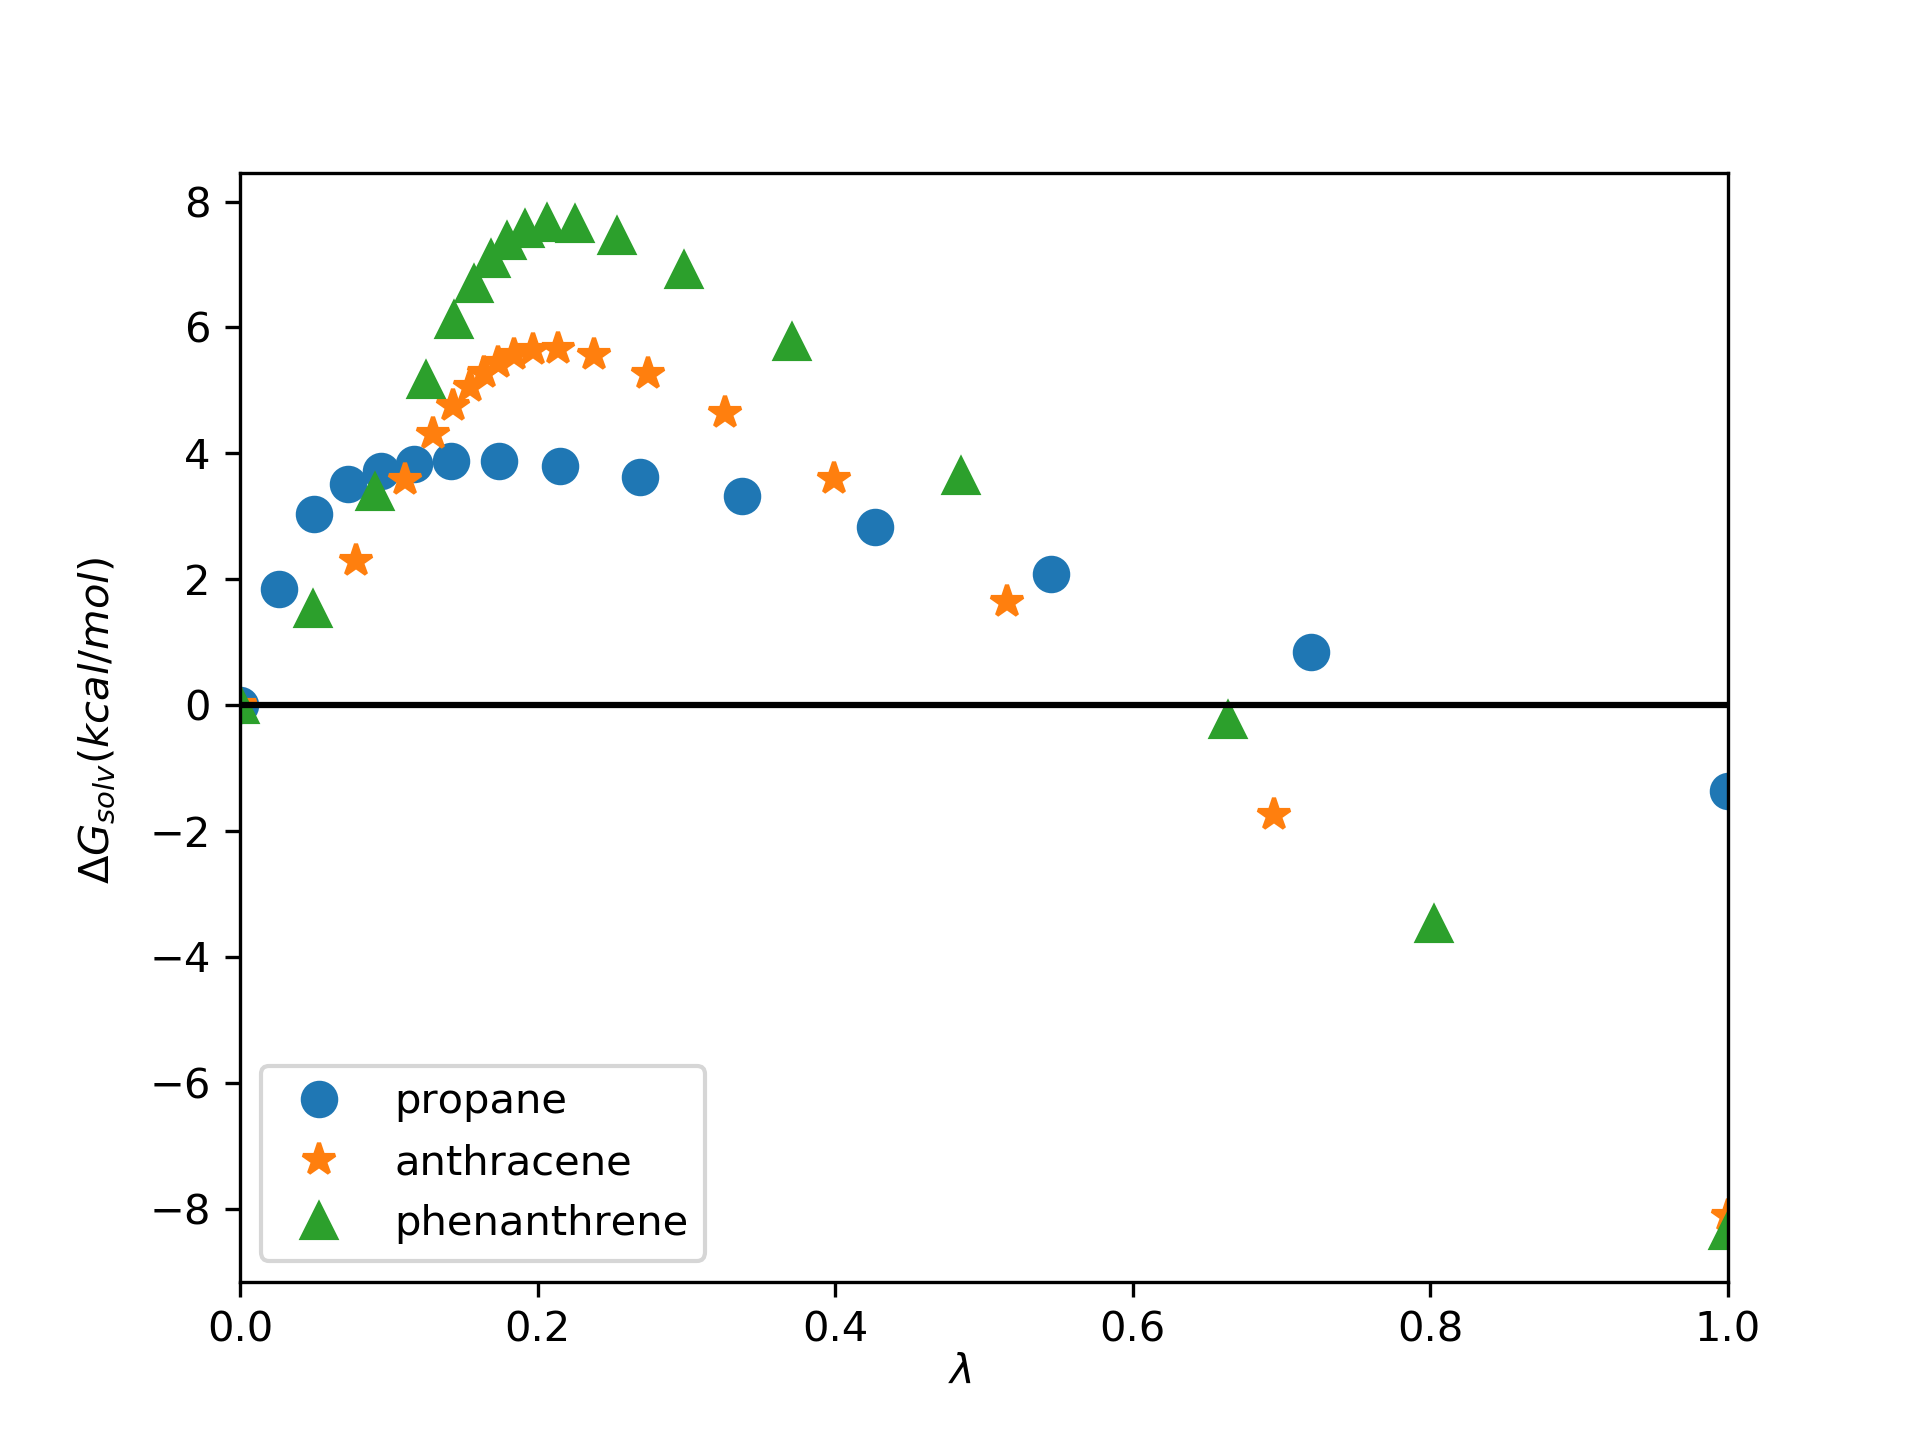
\includegraphics[width=0.8\textwidth]{Figures/oct}
	\caption{Representation of solvation free energies of different solutes in 1-octanol corresponding to each alchemical state.}
	\label{fig:oct}
\end{figure}

\begin{figure}[H]
	\centering
	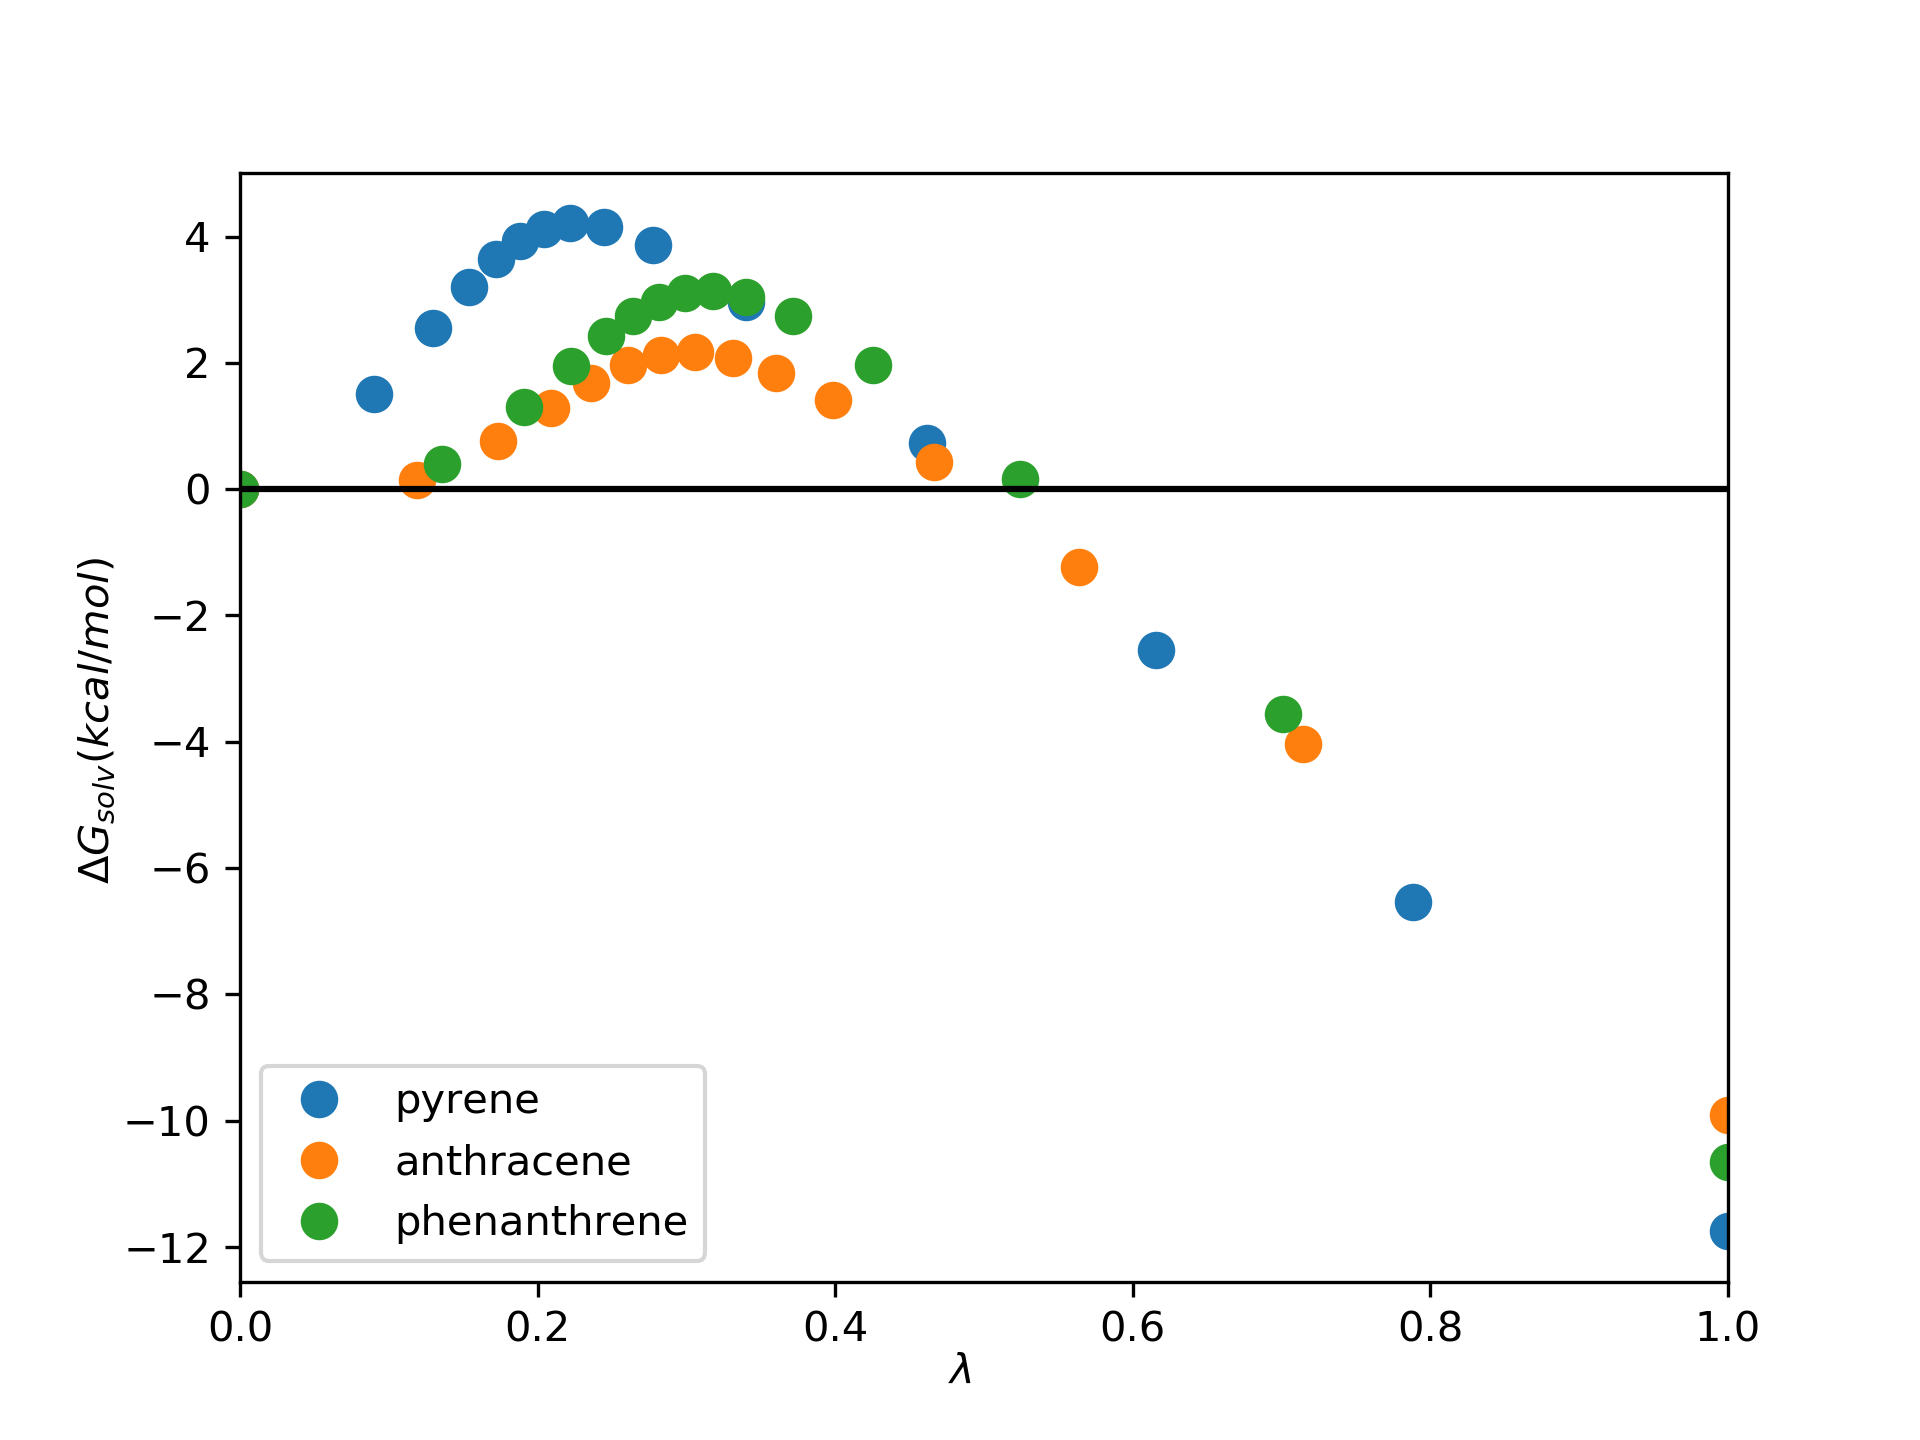
\includegraphics[width=0.8\linewidth]{Figures/tol}
	\caption{Representation of solvation free energies of different solutes in toluene corresponding to each alchemical state. }
	\label{fig:tol}
\end{figure}

The results also indicate a reasonable capability of the force field for predicting the solvation free energies of polyaromatic solutes in aromatic solvents. The influence of the molecular geometry on the solvation free energy curves was the same as the one observed for other solvents, as can be seen in Figure \ref{fig:tol}.  We also calculated the $\Delta G_{solv}$ for phenanthrene in pure toluene and in toluene+$CO_{2}$ mixtures. To the best of our knowledge, there are no available experimental data for these solvation free energies, but the previous results for phenanthrene in other solvents showed that the force field is adequate to describe the solvation phenomenon of phenanthrene in a pure aromatic solvent. Hence, we decided to carry out a qualitative study of the influence of $CO_{2}$ in the solvation free energies of phenanthrene in toluene in order to evaluate the description of this system with the SAFT-$\gamma$ Mie force field. The results for these sets are exposed in Table \ref{tbl:solvco2}.  

\FloatBarrier
\begin{table}[H]
	\centering
	\caption{Calculated values for the solvation free energies (kcal/mol) of phenanthrene in toluene+$CO_{2}$.}
	\label{tbl:solvco2}
	\begin{tabular}{cc}
		\hline
		\hline
		$w_{CO_{2}}$ & $\Delta G_{solv}^{Mie}$ \\
		\hline\hline
		0.0    & -10.65 $\pm$ 0.02   \\
		0.087  & -10.73 $\pm$ 0.02   \\
		0.119  & -10.78 $\pm$ 0.02   \\
		0.169  & -10.71 $\pm$ 0.02   \\
		0.289  & -10.69 $\pm$ 0.02   \\
		\hline
		\hline
	\end{tabular}
\end{table}
\FloatBarrier

The increase of the mass fraction of $CO_{2}$ in toluene caused a small effect on the solvation free energies in the range of weight fractions (0.087-0.289) studied in this dissertation. First, the $\Delta G_{solv}$ decreased with the increase of $w_{CO_{2}}$ up to 0.119. After this, the effect was reversed, and carbon dioxide became an anti-solvent. \citeonline{SOROUSH2014405} reported that asphaltene precipitation occurs when carbon dioxide mass fractions became higher than 0.10 in the system asphaltene+toluene+carbon dioxide, which is in agreement with the anti-solvent effect of carbon dioxide observed in the values calculated here. In the Figure \ref{fig:Figure_1}, we present the free energy profiles of the solvation free energies in the toluene + $CO_{2}$ mixtures. Although we noticed the anti-solvent effect, the differences observed are pretty small. These minor differences may indicate that the effect of $CO_{2}$ is negligible in the solvation of phenanthrene in toluene when using the SAFT-$\gamma$ Mie force field to model the molecules. Nevertheless, more studies need to be done to make a safe assertion about it. It is also worth remarking that this is a qualitative study due to the lack of experimental data. Overall, the methodology proposed by the SAFT-$\gamma$ Mie force field was satisfactory in predicting the solvation free energies of the pairs solvent-solute studied here. For the pair 1-octanol+anthracene, the performance obtained was not as good as it was for the other pairs. This result highlights the importance of choosing a correct geometry for this coarse-grained force field.    

\begin{figure}[H]
	\centering
	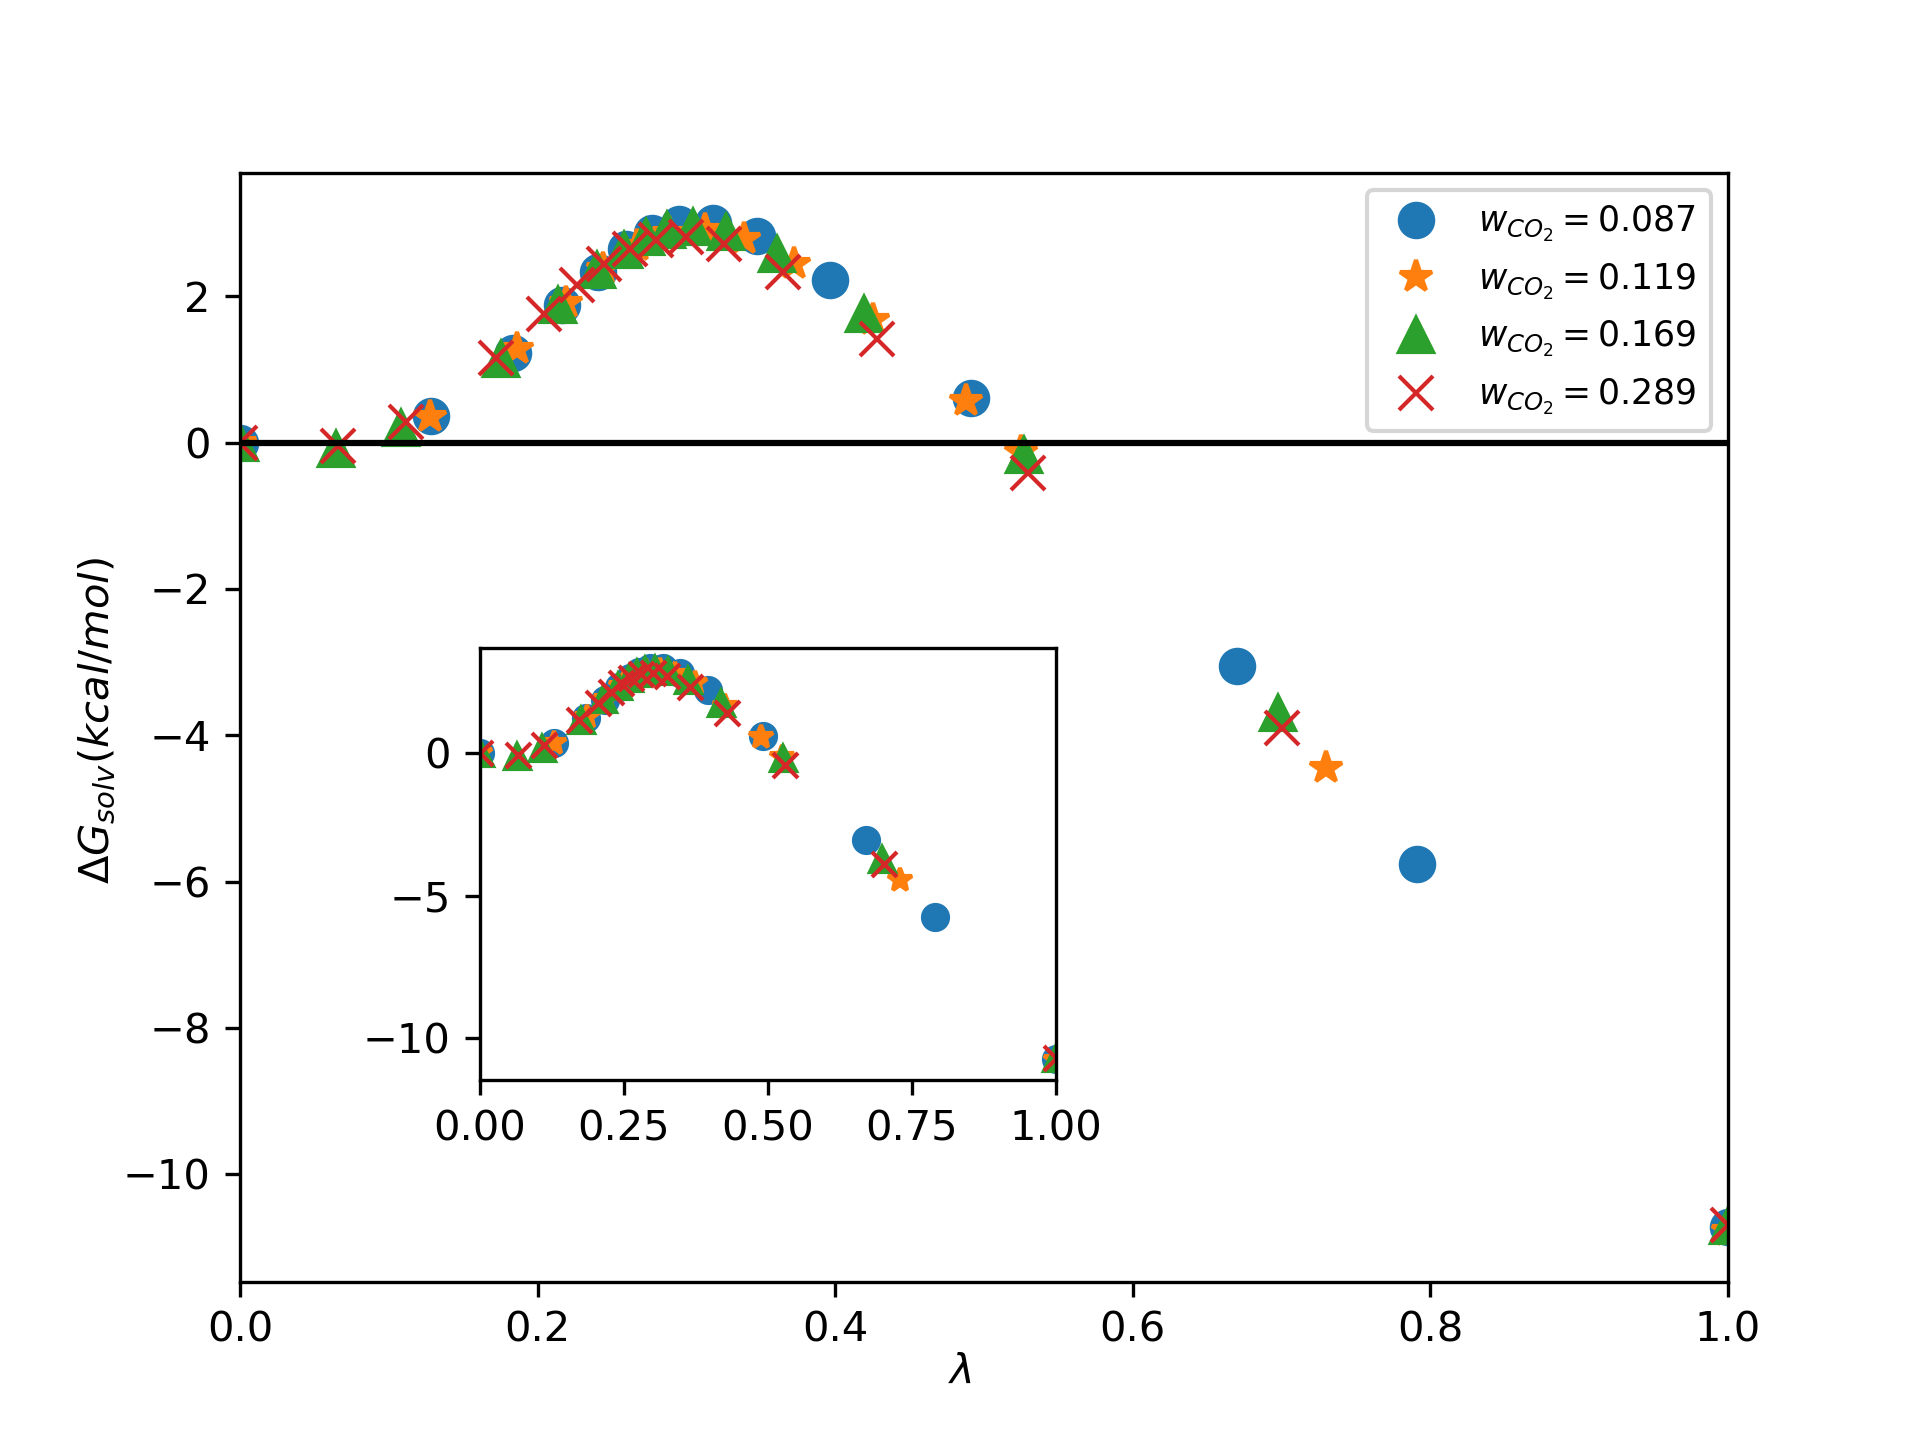
\includegraphics[width=0.8\linewidth]{Figures/tolco2}
	\caption{Representation of solvation free energies of phenanthrene in toluene+$CO_{2}$ corresponding to each alchemical state.}
	\label{fig:Figure_1}
\end{figure}


\section{Hydration free energies}

Water is a solvent extensively used in experimental and computational studies. Because of this importance and the fact that water has unique properties, such as density maximum at 277 K and increased diffusivity upon compression, developing an accurate computational model for water is an ongoing quest \cite{hadley2012}. Hence, we also calculated the solvation free energies in water (hydration free energies) with the SAFT-$\gamma$ Mie force field. With these calculations, we intend to verify if this coarse-grained model would represent the water molecule correctly and would be a good alternative to decrease the computational cost of solvation studies with asphaltene models. The simulations with water as a solvent were carried out using widely studied solutes (propane, benzene) and polyaromatic solutes (toluene, phenanthrene) with a set of fifteen intermediate states.  We obtained these sets of $\lambda$ and $\eta$ with the same methodology used to acquire the sets for the solvation free energies with non-aqueous solvents, and they are exposed in Table \ref{tbl:lambdawater}. At first in our simulations, the binary interaction parameters of all aqueous mixtures were set to zero, but preliminary results for hydration free energies, displayed in Table \ref{tbl:solv3},  exhibited a high deviation from experimental data \cite{P29900000291, doi:10.1021/ct050097l}.

\FloatBarrier
\begin{table*}[h]
	\centering
	\caption{Optimized values of $\lambda $ and $\eta $ for the water+solute pairs. }
	\label{tbl:lambdawater}
	\begin{tabular}{cccccccc}
		\hline\hline
		\multicolumn{2}{c}{propane}& \multicolumn{2}{c}{benzene}& \multicolumn{2}{c}{toluene}& \multicolumn{2}{c}{phenanthrene}\\
		\hline\hline
		$\lambda$ & $\eta$ & $\lambda$ & $\eta$  & $\lambda$ & $\eta$  & $\lambda$ & $\eta$ \\ 
		\hline\hline
		0.000    &    0.000    &    0.000    &    0.000    &    0.000    &    0.000    &    0.000    &    0.000    \\
		0.107    &    2.673    &    0.193    &    -0.295    &    0.177    &    0.182    &    0.142    &    -2.462    \\
		0.157    &    4.703    &    0.279    &    1.468    &    0.262    &    2.432    &    0.256    &    0.597    \\
		0.186    &    6.047    &    0.324    &    2.931    &    0.307    &    4.244    &    0.319    &    4.504    \\
		0.210    &    7.148    &    0.357    &    4.168    &    0.336    &    5.552    &    0.358    &    7.762    \\
		0.230    &    8.017    &    0.381    &    5.091    &    0.360    &    6.696    &    0.384    &    10.104    \\
		0.250    &    8.883    &    0.405    &    5.891    &    0.380    &    7.558    &    0.407    &    12.185    \\
		0.272    &    9.291    &    0.427    &    6.443    &    0.400    &    8.233    &    0.427    &    13.607    \\
		0.294    &    9.700    &    0.449    &    6.770    &    0.422    &    8.678    &    0.446    &    14.490    \\
		0.328    &    9.900    &    0.476    &    6.900    &    0.443    &    8.859    &    0.469    &    14.834    \\
		0.381    &    9.930    &    0.506    &    6.805    &    0.473    &    8.810    &    0.494    &    14.667    \\
		0.484    &    9.463    &    0.555    &    6.392    &    0.514    &    8.452    &    0.533    &    13.832    \\
		0.623    &    8.195    &    0.653    &    5.109    &    0.606    &    7.148    &    0.620    &    11.069    \\
		0.781    &    6.378    &    0.810    &    2.421    &    0.755    &    4.273    &    0.806    &    3.279    \\
		1.000    &    3.333    &    1.000    &    -1.480    &    1.000    &    -1.547    &    1.000    &    -6.122    \\        
		\hline\hline
	\end{tabular}
\end{table*}

\begin{table*}[h]
	\centering
	\caption{Calculated values using $k_{ij}=0$ and experimental values for the hydration free energies (kcal/mol) of solutes in water.}
	\label{tbl:solv3}
	\begin{tabular}{cccc}
		\hline\hline
		Solute       & $\Delta G_{solv}^{exp}$ & $\Delta G_{solv}^{Mie}$ & Absolute Deviation \\ \hline\hline
		propane      & $\,$ 2.00 $\pm$ 0.20         & $\,$ 1.10 $\,$ $\pm$ 0.01         & 0.90               \\
		benzene      & -0.86 $\pm$ 0.20        & -4.45 $\, \,$ $\pm$ 0.03        & 3.59               \\
		toluene      & -0.83 $\pm$ 0.20        & -10.98 $\pm$ 0.30       & 10.15              \\
		phenanthrene & -3.88 $\pm$ 0.60        & -10.90 $\pm$ 0.04       & 7.02               \\ \hline\hline
	\end{tabular}
\end{table*}
\FloatBarrier

With these results, the need for binary interaction parameters became clear. First, we estimated $k_{ij}$ with the SAFT-VR Mie EoS and experimental vapor pressure data, but this strategy also provided results that had high absolute deviations from the experimental data. Therefore, we used the approach of estimating $k_{ij}$ with the output from solvation free energy calculations with molecular dynamics, as described in the last paragraph of Section \ref{solvme}.  We initially found individual values for the interaction parameter of each pair, but, since the parameters for aromatic solutes were very similar (0.148, 0.162, 0.152), we averaged these values. By doing that,  we obtained a general parameter for the water+aromatic pairs, which is exposed in Table \ref{tbl:kij}. Also in this table, we display the binary interaction parameter for the pair water+propane. 

\begin{table*}[h]
	\centering
	\caption{Binary interaction parameters employed.}
	\label{tbl:kij}
	\begin{tabular}{cc}
		\hline
		\hline
		Pair & $k_{ij}$ \\
		\hline\hline
		water+propane      & 0.067  \\
		water+aromatic      & 0.154 \\  
		\hline
		\hline
	\end{tabular}
\end{table*}

The relatively large $k_{ij}$ value of the interaction between aromatic solutes and water can be related to the lack of an explicit association term in the equation of state used to obtain the parameters for water. Actually, the SAFT-VR Mie has an association term \cite{lafitte2013}, but it was not incorporated in the force field. The SAFT-$\gamma$ Mie model for water \cite{lobanova2016} has two different temperature-dependent sets of parameters. The parameters utilized in this work were those estimated with experimental interfacial tension data. Hence, we tested the only binary interaction parameter for water+toluene estimated with MD interfacial data available in the literature \cite{herdes2017}. Nevertheless, the result also had a high absolute deviation, and this parameter could not be transferred to the calculation of the solvation free energy of toluene in water. 

These issues faced by SAFT-$\gamma$ Mie model can also be related to the problems of modeling water with a coarse-grained force field. One of the main difficulties is the choice of which water molecules are going to be represented by which specific beads since water molecules move independently and \DIFdelbegin \DIFdel{are only bound }\DIFdelend \DIFaddbegin \DIFadd{interact }\DIFaddend by non-bonded interactions \cite{hadley2010,hadley2012}. The  SAFT-$\gamma$ Mie water considers that one water molecule corresponds to one bead. This strategy only saves a small amount of simulation time, but it can predict properties at physiological temperatures unlike other more aggressive models such as the MARTINI, which considers that one bead represents various water molecules. In light of all these problems related to modeling the water molecule, the SAFT-$\gamma$ Mie force field appears to be a good alternative when working close to room temperatures, but the necessity of additional parameters estimated with molecular simulation indicates severe flaws in the methodology. This estimation of the binary parameter increased significantly the simulation time required to calculate the hydration free energies, since we had to carry out three additional simulations for every pair water-solute and then three \DIFdelbegin \DIFdel{additional }\DIFdelend \DIFaddbegin \DIFadd{other }\DIFaddend simulations for the three water+polyaromatic solutes in order to test the averaged binary interaction parameter. If these simulations are necessary for every time a new mixture with water is going to be studied with the SAFT-$\gamma$ Mie force field, the use of this model can become impractical.  With this idea in mind, a useful investigation to be made is to check how \DIFdelbegin \DIFdel{much other pairs of water+aromatic solute can be modeled using }\DIFdelend \DIFaddbegin \DIFadd{accurate would be the prediction of the hydration free energy of other aromatic solutes by the SAFT-$\gamma$ Mie force field with }\DIFaddend the binary interaction parameter estimated here. Using these binary interaction parameters calculated with data from molecular dynamics, we then obtained the final hydration free energies presented in Table \ref{tbl:solv2}. 

\begin{table}[H]
	\centering
	\caption{Calculated and experimental hydration free energies  (kcal/mol) of solutes in water.}
	\label{tbl:solv2}
	\begin{tabular}{cccccc}
		\hline\hline
		Solute       & $\Delta G_{solv}^{GAFF}$ & $\Delta G_{solv}^{ELBA}$ & $\Delta G_{solv}^{exp}$ & $\Delta G_{solv}^{Mie}$ & Absolute  \\
		&                          &                          &                         &                         & Deviation \\ \hline\hline
		propane      & 2.50 $\, \pm$0.02           & 2.76 $\, \pm$ 0.02          & 2.00 $\, \pm$ 0.20         & 2.01 $ \, \pm$ 0.01         & 0.01      \\
		benzene      & -0.81$\pm$0.02           & -0.69 $\pm$ 0.01         & -0.86 $\pm$ 0.20        & -1.12 $\pm$ 0.01        & 0.26      \\
		toluene      & -0.79$\pm$0.03           & -0.76 $\pm$ 0.01         & -0.83 $\pm$ 0.20        & -0.84 $\pm$ 0.01        & 0.01      \\
		phenanthrene & -5.26$\pm$0.03           & N/A                        & -3.88 $\pm$ 0.60        & -3.47 $\pm$ 0.02        & 0.41      \\ \hline\hline
		%    RMSE    &                          &                          & 0.24                    &  \\
		%    \hline  &
	\end{tabular}

\end{table}

Hydration free energies calculated using the SAFT-$\gamma$ Mie force field with $k_{ij} \neq 0$ had low absolute deviations from the experimental data, as expected since the parameters were adjusted to fit these experimental data. In the table above, we also show the results obtained by \citeonline{doi:10.1021/acs.jctc.5b00963} with the ELBA force field and by \citeonline{PMID:24928188} with the GAFF force field for the solutes and with the TIP3P model for water. The GAFF (General Amber Force Field) force field is an all-atom model that consists of bonded and non-bonded parameters and is suitable for the study of a significant number of molecules. In turn, the TIP3P model considers that water is a rigid monomer represented by three interacting sites with non-bonded interactions and Coulombic interactions \cite{doi:10.1063/1.445869}. Both the GAFF and the TIP3P models use the Lennard-Jones potential to calculate the non-bonded interactions. \DIFaddbegin \DIFadd{The solvation free energies for the ELBA force field were estimated with thermodynamic integration and the solvation free energies with the GAFF force field were estimated with MBAR.
}\DIFaddend 

Comparing the \DIFaddbegin \DIFadd{results of the }\DIFaddend three aforementioned force fields, the root mean square error (RMSE) of all the pairs tested with the SAFT-$\gamma$ Mie model was  0.24, the RMSE for hydration free energies obtained with the GAFF force field was 0.73, and that for the ELBA coarse-grained force field was 0.44. The difference in absolute deviations between the GAFF and SAFT-$\gamma$ Mie force fields is significantly high for phenanthrene, hence the coarse-grained force field with a binary parameter is preferred if the application requires a high level of accuracy. The results also indicated that the SAFT-$\gamma$ Mie model with the binary interaction parameter performed better than the ELBA force field in modeling the solvation phenomenon of the pairs studied in this work, but performed worse with the binary parameter set to zero. This difference in performance occurred despite the fact that both the SAFT-$\gamma$ Mie and ELBA models have the same level of coarse-graining for the solvent (one bead represents one water molecule). Therefore, the choice between the two coarse-grained models is dependent on the availability and transferability of binary interaction parameters of the Mie Model. We also present, for the SAFT-$\gamma$ Mie force field, the hydration free energy profiles in Figure \ref{fig:water}. Bigger molecules had steeper free energy profiles, as it was for the solvation free energy study in other solvents. We also observe that the hydration free energy for the first non-zero $\lambda$ is negative for benzene and toluene when a positive value is expected since free energy is required \DIFdelbegin \DIFdel{to 'open space' }\DIFdelend \DIFaddbegin \DIFadd{for cavity formation }\DIFaddend in the solvent for the \DIFdelbegin \DIFdel{solute's insertion }\DIFdelend \DIFaddbegin \DIFadd{insertion of the solute}\DIFaddend . This anomaly can be caused by the fact that the exponential parameters in the Mie potential \DIFdelbegin \DIFdel{compensates the need to open space}\DIFdelend \DIFaddbegin \DIFadd{compensate for cavity formation}\DIFaddend . 

\begin{figure}[H]
	\centering
	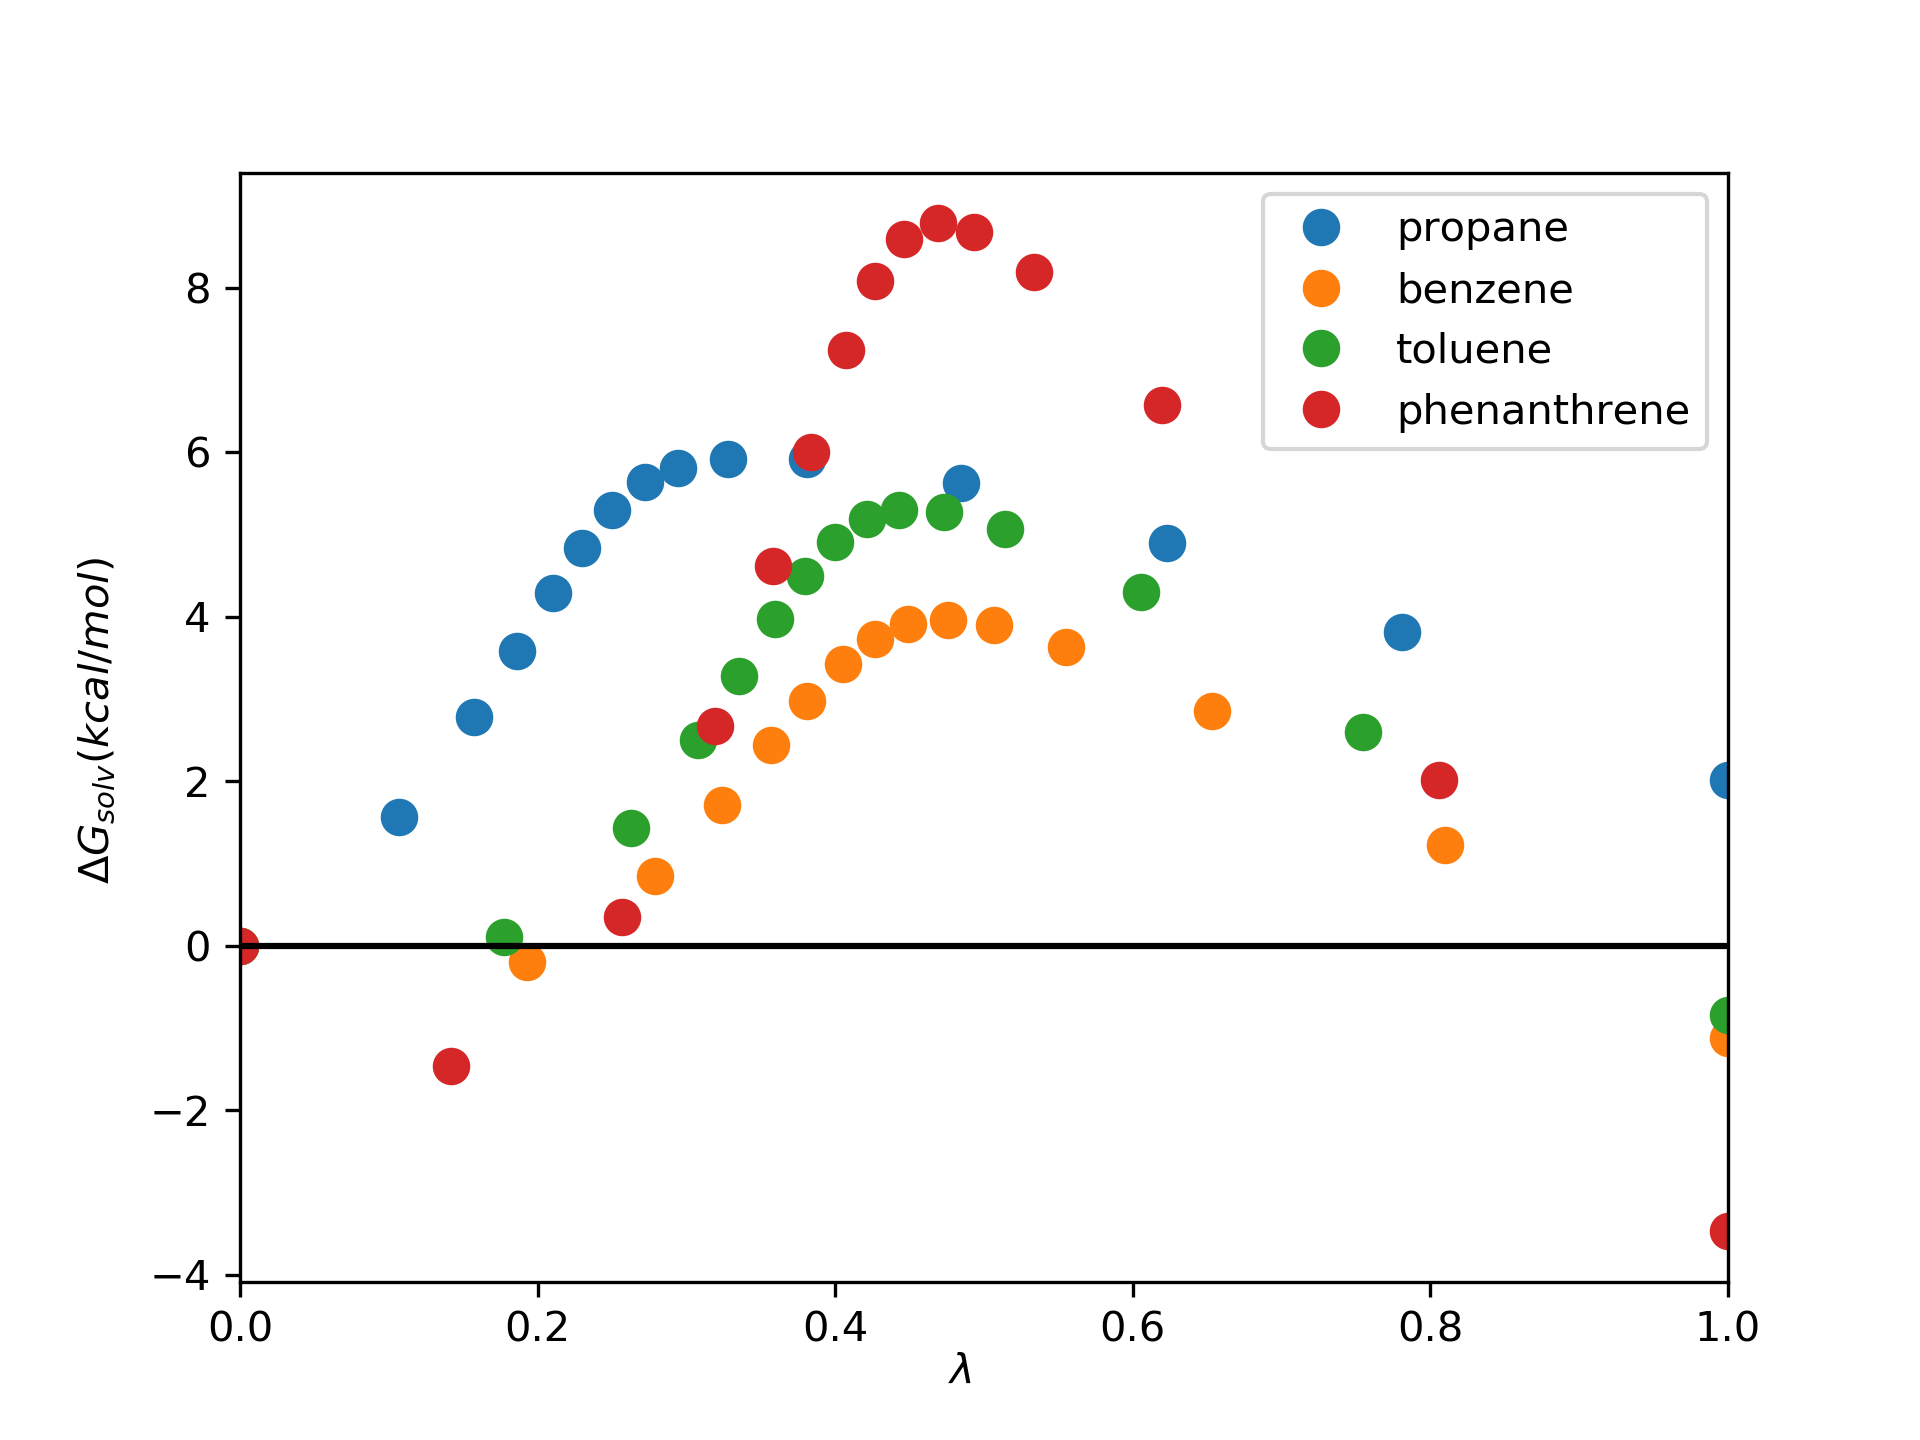
\includegraphics[width=0.8\textwidth]{Figures/water}
	\caption{Representation of hydration free energies of different solutes corresponding to each alchemical state.}
	\label{fig:water}
\end{figure}

The results found here for both the solvation free energies and hydration free energies fulfilled the intentions of this dissertation. We assessed the prediction capability of the SAFT-$\gamma$ Mie force field and provided satisfactory solvation free energy estimates of PAHs using a coarse-grained force field. In addition to that, we found flaws in the methodology used by the SAFT-$\gamma$ Mie force field to model the water molecule. Hence, these shortcomings of this model can now be addressed, and the force field can even be improved by using other mixing rules to avoid the use of a binary parameter or, even, using hydration free energy estimates in the parameterization of water. These results also encourage us to calculate solvation free energies of more complex molecules mimicking asphaltenes in non-aqueous solvents in future studies.  

\section{Partition Coefficients}

Using the solvation free energies estimated in the sections above, we also calculated partition coefficients by means of Eq. \eqref{eqn:partcoe}, for the pairs  water/1-octanol and water/hexane with the intention of testing the modeling capabilities of the SAFT-$\gamma$ Mie force field again. The partition functions studied here have many experimental data available in the literature due to their environmental importance \cite{sangster}. Besides this, the calculations of these specific partition coefficients are relevant because   1-octanol is used to quantify hydrophobicity and can serve as a model for biological lipids and different soils \cite{RUELLE2000457}, and hexane is a model for an apolar, hydrophobic phase. Calculated values and experimental data are shown in Table \ref{tbl:part}. The experimental data of the partition coefficients were taken from   \citeonline{POOLE2000117,sangster} for the coefficient of water/1-octanol and from \citeonline{doi:10.1021/je970112e} for the coefficient of water/hexane. 

\begin{table}[H]
	\centering
	\caption{Partition Coefficient Calculated from MD simulations and from experimental data.}
	\label{tbl:part}
	\begin{tabular}{cccc}
		\hline\hline
		& {Molecular Dynamics} & {Experimental} & Absolute Deviation \\ \hline
		\multicolumn{4}{c}{log $P^{water/1-octanol}$}               \\ \hline
		propane      & 2.47                 & 2.40           & 0.07               \\
		phenanthrene & 3.57                 & 4.46           & 0.89               \\ \hline
		\multicolumn{4}{c}{log $P^{water/hexane}$}                 \\ \hline
		benzene      & 1.93                 & 2.06           & 0.13               \\
		phenanthrene & 4.17                 & 4.49           & 0.32               \\
		%                       \multicolumn{4}{c}{log $P^{tolune/hexane}$}                \\ \hline
		%        pyrene       & -0.67                & -0.97          & 0.30               \\
		%        phenanthrene & -0.47                & -              & -                  \\ 
		\hline\hline
	\end{tabular}

\end{table}

Overall absolute deviations were small for pairs with smaller solvation free energy deviations such as propane and benzene. The water/1-octanol partition coefficient of phenanthrene had higher deviation due to the higher deviation of the free energy of solvation of this compound in 1-octanol. Comparing with other force fields, \citeonline{garrido} reported average absolute deviations for the water/1-octanol partition coefficient of 0.4 with the GROMOS 53a6 force field \cite{JCC:JCC20090}, 0.3 for TraPPE, and 0.9 for OPLS-AA/TraPPE force fields. However, they attribute the low deviations of TraPPE to the cancellation of errors between the two solvation free energies. Additionally, \citeonline{doi:10.1021/acs.jctc.5b00963} found average absolute deviations of 0.86 for the water/hexane partition coefficients and of 0.75 for the water/1-octanol partition coefficients with the ELBA coarse-grained force field. In this dissertation, we performed a small study of partition coefficients with the SAFT-$\gamma$ Mie force field. Hence, a larger set would be necessary to do a complete evaluation of the performance of this force field in the prediction of partition coefficients.   
\DIFdelbegin %DIFDELCMD < 

%DIFDELCMD < %%%
\DIFdelend \chapter{Conclusions} % Main chapter title

\label{Chapter6} 

This dissertation consisted in the study of solvation free energy calculations of aromatic solutes in different solvents by using the SAFT-$\gamma$ Mie coarse-grained force field. Solvation free energy studies are mostly done using water as a solvent and with all-atom force fields based on the Lennard-Jones potential. Therefore, with this study, we were able to provide data about the capability of a coarse-grained force field based on the Mie potential in calculating solvation free energies. Additionally, the solvation free energy estimations carried out here can help improve the SAFT-$\gamma$  Mie force field since these calculations are helpful in identifying errors and shortcomings in the modeling process. The SAFT-$\gamma$ Mie uses the SAFT-VR Mie EoS in its parameterization, which results in a relatively straightforward top-down method of obtaining parameters. Following this strategy, the phenanthrene parameters, which were not available in the original database of this force field, were obtained using vapor-liquid equilibrium data and two different ring equations and geometries. However, only the parameters estimated with the ring equation proposed by \citeonline{muller2017} were utilized in the solvation free energy simulations since this equation did not require molecular simulation data in its parameterization.

To perform our expanded ensemble simulations, we optimized the coupling parameters and their respective simulation weights. The resulting potential energies from the expanded ensemble simulations then served as input to estimate solvation free energy differences with the MBAR method. The results for non-aqueous solvents had absolute deviations from the experimental
data of less than 2.0 kcal/mol, except for the pair 1-octanol+anthracene. We also observed the geometry effect on the free energy curves - larger molecules had steeper curves and more substantial absolute deviations. The influence of carbon dioxide on the solvation free energy of phenanthrene in toluene was found to be negligible according to the SAFT-$\gamma$ Mie force field. 

Hydration free energy calculations with the SAFT-$\gamma$ Mie model required the use of relatively large values of $k_{ij}$ to produce satisfactory results. We chose to estimate the parameter with the output from molecular dynamics data since the strategy of using the SAFT-VR Mie EoS provided high absolute deviations from the experimental data. This necessity of one additional parameter probably happens due to the lack of a term to account for the hydrogen bond in the EoS on which this force field is based and due to problems associated with the coarse-graining of water molecules. The results obtained with $k_{ij}$ estimated with MD output were satisfactory, the absolute deviations from the experimental data found were smaller than the ones for the GAFF and ELBA force fields. We also used the solvation free energies to calculate partition coefficients in water/1-octanol and water/hexane. The obtained absolute deviations from experimental data were similar to the ones found for all-atom force fields (GROMOS, TraPPE and OPLS-AA/TraPPE) and another coarse-grained force field (ELBA).

Overall, the SAFT-$\gamma$ Mie force field proved to be a suitable model to represent the solvation phenomenon of non-aqueous solvents. It correctly described solvation free energies of solutes mimicking asphaltenes dissolved in hexane, toluene, 1-octanol. However, the calculation of hydration free energies required the use of a binary interaction parameter estimated with MD output, which increased the simulation time significantly. This fact evidenced flaws in the methodology used by the SAFT-$\gamma$ force field and raised questions about the feasibility of this model for hydration free energy calculations. Nevertheless, the SAFT-$\gamma$ Mie force field for water used here does not predict freezing at room temperature as other force fields do, which is essential for our hydration free energy calculations. Therefore, it would be relevant to test if the binary interaction parameter for our aromatic solutes estimated here can be used in hydration free energy calculations of other aromatic solutes and if we could use MBAR to obtain the $k_{ij}$ through reweighting. Hence, we would only need to carry out molecular dynamics simulations with one value of $k_{ij}$, and then use this output to estimate with MBAR the results with other $k_{ij} 's $. We also have some ideas that could be developed in the future using the results from this dissertation. The SAFT-$\gamma$ Mie force field could be used to model larger asphaltene models and, consequently, increase the scale of the simulations we performed. Additionally, it would be a valid investigation to study new methodologies to calculate solubility with solvation free energies using the SAFT-$\gamma$ Mie force field.


 


% ----------------------------------------------------------
% ELEMENTOS PÓS-TEXTUAIS
% ----------------------------------------------------------
\postextual
% ----------------------------------------------------------

% ----------------------------------------------------------
% Referências bibliográficas
% ----------------------------------------------------------
\providecommand{\abntreprintinfo}[1]{%
 \citeonline{#1}}
\setlength{\labelsep}{0pt}\begin{thebibliography}{}
\providecommand{\abntrefinfo}[3]{}
\providecommand{\abntbstabout}[1]{}
\abntbstabout{v-1.9.6 }

\bibitem[Abraham \textit{et al.} 1990]{P29900000291}
\abntrefinfo{Abraham \textit{et al.}}{ABRAHAM \textit{et al.}}{1990}
{ABRAHAM, M.~H.; WHITING, G.~S.; FUCHS, R.; CHAMBERS, E.~J. Thermodynamics of
  solute transfer from water to hexadecane.
\emph{Journal of the Chemical Society, Perkin Transactions 2}, p. 291--300,
  1990.}

\bibitem[ABREU 2017]{playmol}
\abntrefinfo{ABREU}{ABREU}{2017}
{ABREU, C. R.~A. \emph{Playmol}. 2017.
  \url{http://atoms.peq.coppe.ufrj.br/playmol /index.html}.
Accessed: 2017-03-10.}

\bibitem[Adam \textit{et al.} 2014]{unres2014}
\abntrefinfo{Adam \textit{et al.}}{ADAM \textit{et al.}}{2014}
{ADAM, L.; MACIEJ, B.; CEZARY, C.; EWA, G.; YI, H.; DAWID, J.; PAWEL, K.;
  MACIEJ, M.; MARIUSZ, M.; A, M.~M.; ANDREI, N.; STANISLAW, O.; A, S.~H.; K,
  S.~A.; RAFAL, S.; TOMASZ, W.; YANPING, Y.; BARTLOMIEJ, Z. A unified
  coarse-grained model of biological macromolecules based on mean-field
  multipole-multipole interactions.
\emph{Journal of molecular modeling}, v.~20, p.~2306, 2014.}

\bibitem[Aimoli \textit{et al.} 2014]{cassiano1}
\abntrefinfo{Aimoli \textit{et al.}}{AIMOLI \textit{et al.}}{2014a}
{AIMOLI, C.~G.; MAGINN, E.~J.; ABREU, C. R.~A. Force field comparison and
  thermodynamic property calculation of supercritical $co_{2}$ and $ch_{4}$
  using molecular dynamics simulations.
\emph{{F}luid {P}hase {E}quilibria}, v.~368, p. 80--90, 2014.}

\bibitem[Aimoli \textit{et al.} 2014]{cassiano2}
\abntrefinfo{Aimoli \textit{et al.}}{AIMOLI \textit{et al.}}{2014b}
{AIMOLI, C.~G.; MAGINN, E.~J.; ABREU, C. R.~A. Transport properties of carbon
  dioxide and methane from molecular dynamics simulations.
\emph{The Journal of Chemical Physics}, v.~141, p. 134101, 2014.}

\bibitem[ANDERSEN 1980]{1980JChPh722384A}
\abntrefinfo{ANDERSEN}{ANDERSEN}{1980}
{ANDERSEN, H.~C. {Molecular dynamics simulations at constant pressure and/or
  temperature}.
\emph{Journal of Chemical Physics}, v.~72, p. 2384--2393, 1980.}

\DIFaddbegin \bibitem[Avenda{\~n}o \textit{et al.} 2013]{doi:10.1021/jp306442b}
\abntrefinfo{Avenda{\~n}o \textit{et al.}}{AVENDA{\~N}O \textit{et al.}}{2013}
{\DIFadd{AVENDA}{\DIFadd{\~N}}\DIFadd{O, C.; LAFITTE, T.; ADJIMAN, C.~S.; GALINDO, A.; MüLLER, E.~A.;
  JACKSON, G. Saft-$\gamma$ force field for the simulation of molecular fluids:
  2. coarse-grained models of greenhouse gases, refrigerants, and long alkanes.
}\emph{\DIFadd{The Journal of Physical Chemistry B}}\DIFadd{, v.~117, n.~9, p. 2717--2733, 2013.}}

\DIFaddend \bibitem[Avenda{\~n}o \textit{et al.} 2011]{avendano2011}
\abntrefinfo{Avenda{\~n}o \textit{et al.}}{AVENDA{\~N}O \textit{et al.}}{2011}
{AVENDA{\~N}O, C.; LAFITTE, T.; GALINDO, A.; ADJIMAN, C.~S.; JACKSON, G.;
  M\"ULLER, E.~A. Saft-$\gamma$ force field for the simulation of molecular
  fluids.1. a single-site coarse grained model of carbon dioxide.
\emph{The Journal of Physical Chemistry B}, v.~115, p. 11154–11169, 2011.}

\bibitem[Barducci \textit{et al.} 2011]{opep2011}
\abntrefinfo{Barducci \textit{et al.}}{BARDUCCI \textit{et al.}}{2011}
{BARDUCCI, A.; BONOMI, M.; DERREUMAUX, P. Assessing the quality of the opep
  coarse-grained force field.
\emph{Journal of Chemical Theory and Computation}, v.~7, p. 1928– 1934,
  2011.}

\bibitem[Barker and Henderson 1976]{bh1976}
\abntrefinfo{Barker and Henderson}{BARKER; HENDERSON}{1976}
{BARKER, J.~A.; HENDERSON, D. What is "liquid"? understanding the states of
  matter.
\emph{Review of Modern Physics}, v.~48, p. 587--671, 1976.}

\bibitem[Basdevant \textit{et al.} 2013]{scorpion2013}
\abntrefinfo{Basdevant \textit{et al.}}{BASDEVANT \textit{et al.}}{2013}
{BASDEVANT, N.; BORGIS, D.; HA-DUONG, T. Modeling protein-protein recognition
  in solution using the coarse-grained force field scorpion.
\emph{Journal of Chemical Theory and Computation}, v.~9, p. 803--813, 2013.}

\bibitem[Beckstein \textit{et al.} 2014]{Beckstein2014}
\abntrefinfo{Beckstein \textit{et al.}}{BECKSTEIN \textit{et al.}}{2014}
{BECKSTEIN, O.; FOURRIER, A.; IORGA, B.~I. Prediction of hydration free
  energies for the sampl4 diverse set of compounds using molecular dynamics
  simulations with the opls-aa force field.
\emph{Journal of Computer-Aided Molecular Design}, v.~28, p. 265--276, 2014.}

\bibitem[Bennett 1976]{bennet1976}
\abntrefinfo{Bennett}{BENNETT}{1976}
{BENNETT, C. Efficient estimation of free energy differences from monte carlo
  data.
\emph{Journal of Computational Physics}, v.~22, p. 245–268, 1976.}

\bibitem[Bereau \textit{et al.} 2010]{bereau2010}
\abntrefinfo{Bereau \textit{et al.}}{BEREAU \textit{et al.}}{2010}
{BEREAU, T.; BACHMANN, M.; DESERNO, M. Interplay between secondary and tertiary
  structure formation in protein folding cooperativity.
\emph{Journal of the American Chemical Society}, v.~132, p. 13129– 13131,
  2010.}

\bibitem[Bereau and Deserno 2009]{bereau2009}
\abntrefinfo{Bereau and Deserno}{BEREAU; DESERNO}{2009}
{BEREAU, T.; DESERNO, M. Generic coarse-grained model for protein folding and
  aggregation.
\emph{Journal of Chemical Physics}, v.~130, p. 235106, 2009.}

\bibitem[Berendsen \textit{et al.} 1984]{doi:10.1063/1.448118}
\abntrefinfo{Berendsen \textit{et al.}}{BERENDSEN \textit{et al.}}{1984}
{BERENDSEN, H. J.~C.; POSTMA, J. P.~M.; GUNSTEREN, W.~F. van; DINOLA, A.; HAAK,
  J.~R. Molecular dynamics with coupling to an external bath.
\emph{The Journal of Chemical Physics}, v.~81, p. 3684--3690, 1984.}

\bibitem[Berg and Neuhaus 1992]{bernd1992}
\abntrefinfo{Berg and Neuhaus}{BERG; NEUHAUS}{1992}
{BERG, B.~A.; NEUHAUS, T. Multicanonical ensemble: A new approach to simulate
  first-order phase transitions.
\emph{Physical Review Letters}, v.~68, p. 9--12, 1992.}

\bibitem[Beutler \textit{et al.} 1994]{beutler1994}
\abntrefinfo{Beutler \textit{et al.}}{BEUTLER \textit{et al.}}{1994}
{BEUTLER, T.; MARK, A.; SCHAIK, R. van; GERBER, P.; GUNSTEREN, W. van. Avoiding
  singularities and numerical instabilities in free energy calculations based
  on molecular simulations.
\emph{Chemical Physics Letters.}, v.~222, p. 529–539, 1994.}

\bibitem[Bhargava and Klein 2009]{bhargava2009}
\abntrefinfo{Bhargava and Klein}{BHARGAVA; KLEIN}{2009}
{BHARGAVA, B.; KLEIN, M.~L. Formation of micelles in aqueous solutions of a
  room temperature ionic liquid: a study using coarse grained molecular
  dynamicss.
\emph{Molecular Simulation}, v.~107, p. 393--401, 2009.}

\bibitem[Buenrostro-Gonzalez \textit{et al.} 2004]{AIC:AIC10243}
\abntrefinfo{Buenrostro-Gonzalez \textit{et al.}}{BUENROSTRO-GONZALEZ
  \textit{et al.}}{2004}
{BUENROSTRO-GONZALEZ, E.; LIRA-GALEANA, C.; GIL-VILLEGAS, A.; WU, J. Asphaltene
  precipitation in crude oils: Theory and experiments.
\emph{AIChE Journal}, v.~50, p. 2552--2570, 2004.}

\bibitem[Chang 1992]{co2toliq}
\abntrefinfo{Chang}{CHANG}{1992}
{CHANG, C.~J. The solubility of carbon dioxide in organic solvents at elevated
  pressures.
\emph{{F}luid {P}hase {E}quilibria}, v.~15, p. 235--242, 1992.}

\bibitem[Chebaro \textit{et al.} 2009]{opep2009}
\abntrefinfo{Chebaro \textit{et al.}}{CHEBARO \textit{et al.}}{2009}
{CHEBARO, Y.; DONG, X.; LAGHAEI, R.; DERREUMAUX, P.; MOUSSEAU, N. Replica
  exchange molecular dynamics simulations of coarse-grained proteins in
  implicit solvent.
\emph{Journal of Physical Chemistry B}, v.~113, p. 267– 274, 2009.}

\bibitem[Chipot and Pohorille 2007]{freeenergy}
\abntrefinfo{Chipot and Pohorille}{CHIPOT; POHORILLE}{2007}
{CHIPOT, C.; POHORILLE, A. \emph{Free Energy Calculations Theory and
  Applications in Chemistry and Biology}. 1. ed. New York: Springer, 2007.}

\bibitem[Chiu \textit{et al.} 2010]{chiu2010}
\abntrefinfo{Chiu \textit{et al.}}{CHIU \textit{et al.}}{2010}
{CHIU, S.~W.; SCOTT, H.~L.; JAKOBSSON, E. A coarse-grained model based on morse
  potential for water and n-alkanes.
\emph{Journal of Chemical Theory and Computation}, v.~6, p. 851--863, 2010.}

\bibitem[Chodera and Shirts 2011]{chodera2011}
\abntrefinfo{Chodera and Shirts}{CHODERA; SHIRTS}{2011}
{CHODERA, J.~D.; SHIRTS, M.~R. Replica exchange and expanded ensemble
  simulations as gibbs sampling: simple improvements for enhanced mixing.
\emph{Journal of Chemical Physics}, v.~135, p. 194110, 2011.}

\bibitem[Dayal \textit{et al.} 2004]{dayal2004}
\abntrefinfo{Dayal \textit{et al.}}{DAYAL \textit{et al.}}{2004}
{DAYAL, P.; TREBST, S.; WESSEL, S.; W\"URTZ, D.; TROYER, M.; SABHAPANDIT, S.;
  COPPERSMITH, S.~N. Performance limitations of flat-histogram methods.
\emph{Physical Review Letters}, v.~92, p. 097201, 2004.}

\bibitem[Ervik \textit{et al.} 2016]{ervik20162}
\abntrefinfo{Ervik \textit{et al.}}{ERVIK \textit{et al.}}{2016a}
{ERVIK, A.; LYSGAARD, M.~O.; HERDES, C.; JIM\'ENEZ-SERRATOS, G.; M\"LLER,
  E.~A.; MUNKEJORD, S.~T.; M\"ULLER, B. A multiscale method for simulating
  fluid interfaces covered with large molecules such as asphaltenes.
\emph{Journal of Computational Physics}, v.~327, p. 576--611, 2016.}

\bibitem[Ervik \textit{et al.} 2016]{ervik2016}
\abntrefinfo{Ervik \textit{et al.}}{ERVIK \textit{et al.}}{2016b}
{ERVIK, A.; MEJ\'IA, A.; M\"ULLER, E.~A. Bottled saft: A web app providing
  saft-$\gamma$ mie force field parameters for thousands of molecular fluids.
\emph{Journal of Chemical Information and Modeling}, v.~56, p. 1609–1614,
  2016.}

\bibitem[Escobedo and Martinez-Veracoechea 2007]{escobedo2007}
\abntrefinfo{Escobedo and Martinez-Veracoechea}{ESCOBEDO;
  MARTINEZ-VERACOECHEA}{2007}
{ESCOBEDO, F.~A.; MARTINEZ-VERACOECHEA, F.~J. Optimized expanded ensembles for
  simulations involving molecular insertions and deletions. i. closed systems.
\emph{Journal of Chemical Physics}, v.~127, p. 174103, 2007.}

\bibitem[Essex \textit{et al.} 1992]{doi:10.1021/ja00036a009}
\abntrefinfo{Essex \textit{et al.}}{ESSEX \textit{et al.}}{1992}
{ESSEX, J.~W.; REYNOLDS, C.~A.; RICHARDS, W.~G. Theoretical determination of
  partition coefficients.
\emph{Journal of the American Chemical Society}, v.~114, p. 3634--3639, 1992.}

\bibitem[Ferrenberg and Swendsen 1989]{PhysRevLett.63.1195}
\abntrefinfo{Ferrenberg and Swendsen}{FERRENBERG; SWENDSEN}{1989}
{FERRENBERG, A.~M.; SWENDSEN, R.~H. Optimized monte carlo data analysis.
\emph{Physical Review Letters}, v.~63, p. 1195--1198, 1989.}

\bibitem[Frenkel 2013]{Frenkel2013}
\abntrefinfo{Frenkel}{FRENKEL}{2013}
{FRENKEL, D. Simulations: The dark side.
\emph{The European Physical Journal Plus}, v.~128, p.~10, 2013.}

\bibitem[Frenkel and Smit 2001]{frenkel}
\abntrefinfo{Frenkel and Smit}{FRENKEL; SMIT}{2001}
{FRENKEL, D.; SMIT, B. \emph{Understanding Molecular Simulation}. 2nd. ed.
  Orlando, FL, USA: Academic Press, Inc., 2001.}

\bibitem[Gao \textit{et al.} 2014]{doi:10.1021/ef5020428}
\abntrefinfo{Gao \textit{et al.}}{GAO \textit{et al.}}{2014}
{GAO, F.; XU, Z.; LIU, G.; YUAN, S. Molecular dynamics simulation: The behavior
  of asphaltene in crude oil and at the oil/water interface.
\emph{Energy \& Fuels}, v.~28, p. 7368--7376, 2014.}

\bibitem[Garrido \textit{et al.} 2011]{garrido2011}
\abntrefinfo{Garrido \textit{et al.}}{GARRIDO \textit{et al.}}{2011}
{GARRIDO, N.~M.; JORGE, M.; QUEIMADA, A.~J.; MACEDO, E.~A.; ECONOMOU, I.~G.
  Using molecular simulation to predict solute solvation and partition
  coefficients in solvents of different polarity.
\emph{Physical Chemistry Chemical Physics}, v.~20, p. 9155--9164, 2011.}

\bibitem[Garrido \textit{et al.} 2009]{garrido}
\abntrefinfo{Garrido \textit{et al.}}{GARRIDO \textit{et al.}}{2009}
{GARRIDO, N.~M.; QUEIMADA, A.~J.; JORGE, M.; MACEDO, E.~A.; ECONOMOU, I.~G.
  1-octanol/water partition coefficients of n-alkanes from molecular
  simulations of absolute solvation free energies.
\emph{Journal of Chemical Theory and Computation}, v.~5, p. 2436--2446, 2009.}

\bibitem[Geman and Geman 1984]{geman1984}
\abntrefinfo{Geman and Geman}{GEMAN; GEMAN}{1984}
{GEMAN, S.; GEMAN, D. Stochastic relaxation, gibbs distributions, and the
  bayesian restoration of images.
\emph{IEEE Transactions on Pattern Analysis and Machine Intelligence}, PAMI-6,
  p. 721 -- 741, 1984.}

\bibitem[Genheden 2016]{doi:10.1021/acs.jctc.5b00963}
\abntrefinfo{Genheden}{GENHEDEN}{2016}
{GENHEDEN, S. Predicting partition coefficients with a simple
  all-atom/coarse-grained hybrid model.
\emph{Journal of Chemical Theory and Computation}, v.~12, p. 297--304, 2016.}

\bibitem[Gon{\c c}alves and Stassen 2005]{goncalves}
\abntrefinfo{Gon{\c c}alves and Stassen}{GON{\c C}ALVES; STASSEN}{2005}
{GON{\c C}ALVES, P. F.~B.; STASSEN, H. Free energy of solvation from molecular
  dynamics simulation applying voronoi-delaunay triangulation to the cavity
  creation.
\emph{The Journal of Chemical Physics}, v.~123, p. 214109, 2005.}

\bibitem[Greenfield 2011]{doi:10.1080/10298436.2011.575141}
\abntrefinfo{Greenfield}{GREENFIELD}{2011}
{GREENFIELD, M.~L. Molecular modelling and simulation of asphaltenes and
  bituminous materials.
\emph{International Journal of Pavement Engineering}, v.~12, p. 325--341,
  2011.}

\bibitem[Hadley and McCabe 2010]{hadley2010}
\abntrefinfo{Hadley and McCabe}{HADLEY; MCCABE}{2010}
{HADLEY, K.~R.; MCCABE, C. On the investigation of coarse-grained models for
  water: Balancing computational efficiency and the retention of structural
  properties.
\emph{The Journal of Physical Chemistry B}, v.~114, p. 4590--4599, 2010.}

\bibitem[Hadley and McCabe 2012]{hadley2012}
\abntrefinfo{Hadley and McCabe}{HADLEY; MCCABE}{2012}
{HADLEY, K.~R.; MCCABE, C. Coarse-grained molecular models of water: a review.
\emph{Molecular Simulation}, v.~38, p. 671–681, 2012.}

\bibitem[He \textit{et al.} 2010]{shinoda2010}
\abntrefinfo{He \textit{et al.}}{HE \textit{et al.}}{2010}
{HE, X.; SHINODA, W.; DEVANE, R.; KLEIN, M.~L. Exploring the utility of
  coarse-grained water models for computational studies of interfacial systems.
\emph{Molecular Simulation}, v.~108, p. 2007--2020, 2010.}

\bibitem[Headen \textit{et al.} 2017]{doi:10.1021/acs.energyfuels.6b02161}
\abntrefinfo{Headen \textit{et al.}}{HEADEN \textit{et al.}}{2017}
{HEADEN, T.~F.; BOEK, E.~S.; JACKSON, G.; TOTTON, T.~S.; MüLLER, E.~A.
  Simulation of asphaltene aggregation through molecular dynamics: Insights and
  limitations.
\emph{Energy \& Fuels}, v.~31, p. 1108--1125, 2017.}

\bibitem[Herdes \textit{et al.} 2017]{herdes2017}
\abntrefinfo{Herdes \textit{et al.}}{HERDES \textit{et al.}}{2017}
{HERDES, C.; ERVIK, A.; MEJ\'IA, A.; M\"ULLER, E.~A. Prediction of the
  water/oil interfacial tension from molecular simulations using the
  coarse-grained saft-$\gamma$ mie force field.
\emph{{F}luid {P}hase {E}\DIFdelbegin \DIFdel{quilib.}\DIFdelend \DIFaddbegin \DIFadd{quilibria}\DIFaddend }, 2017.}

\bibitem[Herdes \textit{et al.} 2015]{herdes2015}
\abntrefinfo{Herdes \textit{et al.}}{HERDES \textit{et al.}}{2015}
{HERDES, C.; TOTTON, T.~S.; M\"ULLER, E.~A. Coarse grained force field for the
  molecular simulation of natural gases and condensates.
\emph{Fluid Phase Equilibria}, v.~406, p. 91–100, 2015.}

\bibitem[Hoover 1985]{PhysRevA.31.1695}
\abntrefinfo{Hoover}{HOOVER}{1985}
{HOOVER, W.~G. Canonical dynamics: Equilibrium phase-space distributions.
\emph{Physical Review A}, v.~31, p. 1695--1697, 1985.}

\bibitem[Izairi and Kamberaj 2017]{izairi2017}
\abntrefinfo{Izairi and Kamberaj}{IZAIRI; KAMBERAJ}{2017}
{IZAIRI, R.; KAMBERAJ, H. Comparison study of polar and nonpolar contributions
  to solvation free energy.
\emph{Journal of Chemical Information and Modeling}, v.~57, p. 2539–2553,
  2017.}

\bibitem[Jorge \textit{et al.} 2010]{garrido2010}
\abntrefinfo{Jorge \textit{et al.}}{JORGE \textit{et al.}}{2010}
{JORGE, M.; GARRIDO, N.; QUEIMADA, A.; ECONOMOU, I.; MACEDO, E. Effect of the
  integration method on the accuracy and computational efficiency of free
  energy calculations using thermodynamic integration.
\emph{Journal of Chemical Theory and Computation}, v.~6, p. 1018–1027, 2010.}

\bibitem[Jorgensen \textit{et al.} 1983]{doi:10.1063/1.445869}
\abntrefinfo{Jorgensen \textit{et al.}}{JORGENSEN \textit{et al.}}{1983}
{JORGENSEN, W.~L.; CHANDRASEKHAR, J.; MADURA, J.~D.; IMPEY, R.~W.; KLEIN, M.~L.
  Comparison of simple potential functions for simulating liquid water.
\emph{The Journal of Chemical Physics}, v.~79, p. 926--935, 1983.}

\bibitem[Jorgensen and Tirado-Rives 1988]{doi:10.1021/ja00214a001}
\abntrefinfo{Jorgensen and Tirado-Rives}{JORGENSEN; TIRADO-RIVES}{1988}
{JORGENSEN, W.~L.; TIRADO-RIVES, J. The opls [optimized potentials for liquid
  simulations] potential functions for proteins, energy minimizations for
  crystals of cyclic peptides and crambin.
\emph{Journal of the American Chemical Society}, v.~110, p. 1657--1666, 1988.}

\bibitem[Joshi \textit{et al.} 2001]{doi:10.1021/ef010047l}
\abntrefinfo{Joshi \textit{et al.}}{JOSHI \textit{et al.}}{2001}
{JOSHI, N.~B.; MULLINS, O.~C.; JAMALUDDIN, A.; CREEK, J.; MCFADDEN, J.
  Asphaltene precipitation from live crude oil.
\emph{Energy \& Fuels}, v.~15, p. 979--986, 2001.}

\bibitem[Jover \textit{et al.} 2015]{doi:10.1021/ef502209j}
\abntrefinfo{Jover \textit{et al.}}{JOVER \textit{et al.}}{2015}
{JOVER, J.~F.; MüLLER, E.~A.; HASLAM, A.~J.; GALINDO, A.; JACKSON, G.;
  TOULHOAT, H.; NIETO-DRAGHI, C. Aspects of asphaltene aggregation obtained
  from coarse-grained molecular modeling.
\emph{Energy \& Fuels}, v.~29, p. 556--566, 2015.}

\bibitem[Kamberaj \textit{et al.} 2005]{kamberaj}
\abntrefinfo{Kamberaj \textit{et al.}}{KAMBERAJ \textit{et al.}}{2005}
{KAMBERAJ, H.; LOW, R.; NEAL, M. Time reversible and symplectic integrators for
  molecular dynamics simulations of rigid molecules.
\emph{Journal of Chemical Physics}, v.~122, p. 224114, 2005.}

\bibitem[Katritzky \textit{et al.} 2003]{doi:10.1021/ci034120c}
\abntrefinfo{Katritzky \textit{et al.}}{KATRITZKY \textit{et al.}}{2003}
{KATRITZKY, A.~R.; OLIFERENKO, A.~A.; OLIFERENKO, P.~V.; PETRUKHIN, R.; TATHAM,
  D.~B.; MARAN, U.; LOMAKA, A.; ACREE, W.~E. A general treatment of solubility.
  1. the qspr correlation of solvation free energies of single solutes in
  series of solvents.
\emph{Journal of Chemical Information and Modeling}, v.~43, p. 1794--1805,
  2003.}

\bibitem[Katzgraber \textit{et al.} 2006]{1742-5468-2006-03-P03018}
\abntrefinfo{Katzgraber \textit{et al.}}{KATZGRABER \textit{et al.}}{2006}
{KATZGRABER, H.~G.; TREBST, S.; HUSE, D.~A.; TROYER, M. Feedback-optimized
  parallel tempering monte carlo.
\emph{Journal of Statistical Mechanics: Theory and Experiment}, v.~2006, p.
  P03018, 2006.}

\bibitem[Kirkwood 1935]{kirkwood1935}
\abntrefinfo{Kirkwood}{KIRKWOOD}{1935}
{KIRKWOOD, J. Statistical mechanics of fluid mixtures.
\emph{Journal of Chemical Physics}, v.~3, p. 300–313, 1935.}

\bibitem[Klimovich \textit{et al.} 2015]{klimovich}
\abntrefinfo{Klimovich \textit{et al.}}{KLIMOVICH \textit{et al.}}{2015}
{KLIMOVICH, P.~V.; SHIRTS, M.~R.; MOBLEY, D.~L. Guidelines for the analysis of
  free energy calculations.
\emph{Journal of Computer-Aided Molecular Design}, v.~29, p. 397--411, 2015.}

\bibitem[Kmiecik \textit{et al.} 2016]{kmiecik2016}
\abntrefinfo{Kmiecik \textit{et al.}}{KMIECIK \textit{et al.}}{2016}
{KMIECIK, S.; GRONT, D.; KOLINSKI, M.; WIETESKA, L.; DAWID, A.~E.; KOLINSKI, A.
  Coarse-grained protein models and their applications.
\emph{Chemical Reviews}, v.~116, p. 7898–7936, 2016.}

\bibitem[Kobryn and Kovalenko 2008]{doi:10.1063/1.2972978}
\abntrefinfo{Kobryn and Kovalenko}{KOBRYN; KOVALENKO}{2008}
{KOBRYN, A.~E.; KOVALENKO, A. Molecular theory of hydrodynamic boundary
  conditions in nanofluidics.
\emph{The Journal of Chemical Physics}, v.~129, p. 134701, 2008.}

\bibitem[Koga and Takada 2001]{koga2001}
\abntrefinfo{Koga and Takada}{KOGA; TAKADA}{2001}
{KOGA, N.; TAKADA, S. Roles of native topology and chain-length scaling in
  protein folding: a simulation study with a go-like model.
\emph{Journal of Molecular Biology}, v.~331, p. 171–180, 2001.}

\bibitem[Kumar \textit{et al.} 1992]{wham}
\abntrefinfo{Kumar \textit{et al.}}{KUMAR \textit{et al.}}{1992}
{KUMAR, S.; BOUZIDA, D.; SWENDSEN, R.; KOLLMAN, P.; ROSENBERG, J. The weighted
  histogram analysis method for free-energy calculations on biomolecules. 1.
  the method.
\emph{Journal of Computational Chemistry}, v.~13, p. 1011--1021, 1992.}

\bibitem[Kuznicki \textit{et al.} 2009]{doi:10.1021/ef9004576}
\abntrefinfo{Kuznicki \textit{et al.}}{KUZNICKI \textit{et al.}}{2009}
{KUZNICKI, T.; MASLIYAH, J.~H.; BHATTACHARJEE, S. Aggregation and partitioning
  of model asphaltenes at toluene - water interfaces: Molecular dynamics
  simulations.
\emph{Energy \& Fuels}, v.~23, p. 5027–5035, 2009.}

\bibitem[Lafitte \textit{et al.} 2013]{lafitte2013}
\abntrefinfo{Lafitte \textit{et al.}}{LAFITTE \textit{et al.}}{2013}
{LAFITTE, T.; APOSTOLAKOU, A.; AVENDANO, C.; GALINDO, A.; ADJIMAN, C.~S.;
  MULLER, E.~A.; JACKSON, G. Accurate statistical associating fluid theory for
  chain molecules formed from mie segments.
\emph{The Journal of Chemical Physics}, v.~139, p. 154504, 2013.}

\bibitem[Lafitte \textit{et al.} 2012]{lafitte2012}
\abntrefinfo{Lafitte \textit{et al.}}{LAFITTE \textit{et al.}}{2012}
{LAFITTE, T.; AVENDA{\~N}O, C.; PAPAIOANNOU, V.; GALINDO, A.; ADJIMAN, C.~S.;
  JACKSON, G.; M\"ULLER, E.~A. Saft-$\gamma$ force field for the simulation of
  molecular fluids: 3. coarse-grained models of benzene and hetero-group models
  of n-decylbenzene.
\emph{Molecular Physics}, v.~110, p. 1189–1203, 2012.}

\bibitem[Lars \textit{et al.} 2013]{martini2013}
\abntrefinfo{Lars \textit{et al.}}{LARS \textit{et al.}}{2013}
{LARS, V.; PERIOLE, X.; TIELEMAN, D.~P.; MARRINK, S.~J. Improved parameters for
  the martini coarse-grained protein force field.
\emph{Journal of Chemical Theory and Computation}, v.~9, p. 687--697, 2013.}

\bibitem[Lee 1993]{bernd1993}
\abntrefinfo{Lee}{LEE}{1993}
{LEE, J. New monte carlo algorithm: Entropic sampling.
\emph{Physical Review Letters}, v.~71, p. 211--214, 1993.}

\bibitem[Levitt 1976]{levitt1976}
\abntrefinfo{Levitt}{LEVITT}{1976}
{LEVITT, M. A simplified representation of protein conformations for rapid
  simulation of protein folding.
\emph{Journal of Molecular Biology}, v.~104, p. 59--107, 1976.}

\DIFdelbegin %DIFDELCMD < \bibitem[Levitt and Warshe 1975]{levitt1975}
%DIFDELCMD < \abntrefinfo{Levitt and Warshe}{LEVITT; WARSHE}{1975}
%DIFDELCMD < %%%
\DIFdelend \DIFaddbegin \bibitem[Levitt and Warshel 1975]{levitt1975}
\abntrefinfo{Levitt and Warshel}{LEVITT; WARSHEL}{1975}
\DIFaddend {LEVITT, M.; \DIFdelbegin \DIFdel{WARSHE}\DIFdelend \DIFaddbegin \DIFadd{WARSHEL}\DIFaddend , A. Computer-simulation of protein folding.
\emph{Nature}, v.~253, p. 694–698, 1975.}

\bibitem[Li and Greenfield 2011]{doi:10.1021/ef200507c}
\abntrefinfo{Li and Greenfield}{LI; GREENFIELD}{2011}
{LI, D.~D.; GREENFIELD, M.~L. High internal energies of proposed asphaltene
  structures.
\emph{Energy \& Fuels}, v.~25, p. 3698--3705, 2011.}

\bibitem[Liu 2002]{liu2002}
\abntrefinfo{Liu}{LIU}{2002}
{LIU, J.~S. \emph{Monte Carlo strategies in Scientific Computing}. 2. ed. New
  York: Springer, 2002.}

\bibitem[Lobanova \textit{et al.} 2015]{lobanova2015}
\abntrefinfo{Lobanova \textit{et al.}}{LOBANOVA \textit{et al.}}{2015}
{LOBANOVA, O.; AVENDA{\~N}O, C.; LAFITTE, T.; M\"ULLER, E.~A.; JACKSON, G.
  Saft-$\gamma$ force field for the simulation of molecular fluids: 4. a
  single-site coarse-grained model of water applicable over a wide temperature
  range.
\emph{Molecular Physics}, v.~113, p. 1228–1249, 2015.}

\bibitem[Lobanova \textit{et al.} 2016]{lobanova2016}
\abntrefinfo{Lobanova \textit{et al.}}{LOBANOVA \textit{et al.}}{2016}
{LOBANOVA, O.; MEJ\'IA, A.; JACKSON, G.; M\"LLER, E.~A. Saft-$\gamma$ force
  field for the simulation of molecular fluids 6: Binaryand ternary mixtures
  comprising water, carbon dioxide, and n-alkanes.
\emph{The Journal of Chemical Thermodynamics}, v.~93, p. 320–336, 2016.}

\bibitem[Lyubartsev \textit{et al.} 1992]{lyubartsev}
\abntrefinfo{Lyubartsev \textit{et al.}}{LYUBARTSEV \textit{et al.}}{1992}
{LYUBARTSEV, A.~P.; MARTSINOVSKI, A.~A.; SHEVKUNOV, S.~V.;
  VORONTSOV‐VELYAMINOV, P.~N. New approach to monte carlo calculation of the
  free energy: Method of expanded ensembles.
\emph{Journal of Chemical Physics}, v.~96, p. 1776--1783, 1992.}

\bibitem[Marrink \textit{et al.} 2007]{martini2007}
\abntrefinfo{Marrink \textit{et al.}}{MARRINK \textit{et al.}}{2007}
{MARRINK, S.~J.; RISSELADA, H.~J.; YEFIMOV, S.; TIELEMAN, D.~P.; VRIES, A.~H.
  de. The martini force field: Coarse grained model for biomolecular
  simulations.
\emph{Journal of Physical Chemistry B}, v.~111, p. 7812–7824, 2007.}

\bibitem[Marrink and Tieleman 2013]{martini20132}
\abntrefinfo{Marrink and Tieleman}{MARRINK; TIELEMAN}{2013}
{MARRINK, S.~J.; TIELEMAN, D.~P. Perspective on the martini model.
\emph{Chemical Society Reviews}, v.~42, p. 6801– 6822, 2013.}

\bibitem[Mart\'inez \textit{et al.} 2009]{packmol}
\abntrefinfo{Mart\'inez \textit{et al.}}{MART\'INEZ \textit{et al.}}{2009}
{MART\'INEZ, L.; ANDRADE, R.; BIRGIN, E.~G.; MART\'INEZ, J.~M. Packmol: a
  package for building initial configurations for molecular dynamics
  simulations.
\emph{Journal of Computational Chemistry}, v.~30, p. 2157--2164, 2009.}

\bibitem[Martyna \textit{et al.} 1992]{doi:10.1063/1.463940}
\abntrefinfo{Martyna \textit{et al.}}{MARTYNA \textit{et al.}}{1992}
{MARTYNA, G.~J.; KLEIN, M.~L.; TUCKERMAN, M. Nos\'e - hoover chains: The
  canonical ensemble via continuous dynamics.
\emph{The Journal of Chemical Physics}, v.~97, p.~2635, 1992.}

\bibitem[Martyna \textit{et al.} 1994]{doi:10.1063/1.467468}
\abntrefinfo{Martyna \textit{et al.}}{MARTYNA \textit{et al.}}{1994}
{MARTYNA, G.~J.; TOBIAS, D.~J.; KLEIN, M.~L. Constant pressure molecular
  dynamics algorithms.
\emph{The Journal of Chemical Physics}, v.~101, p. 4177--4189, 1994.}

\bibitem[Matos \textit{et al.} 2017]{mobley2017}
\abntrefinfo{Matos \textit{et al.}}{MATOS \textit{et al.}}{2017}
{MATOS, G. D.~R.; KYU, D.~Y.; LOEFFLER, H.~H.; CHODERA, J.~D.; SHIRTS, M.~R.; ;
  MOBLEY, D.~L. Approaches for calculating solvation free energies and
  enthalpies demonstrated with an update of the freesolv database.
\emph{Journal Chemical Engineering Data}, v.~62, p. 1559--1569, 2017.}

\bibitem[Matubayasi 2017]{MATUBAYASI201745}
\abntrefinfo{Matubayasi}{MATUBAYASI}{2017}
{MATUBAYASI, N. Free-energy analysis of protein solvation with all-atom
  molecular dynamics simulation combined with a theory of solutions.
\emph{Current Opinion in Structural Biology}, v.~43, p. 45 -- 54, 2017.}

\bibitem[Mej\'ia \textit{et al.} 2014]{mejia2014}
\abntrefinfo{Mej\'ia \textit{et al.}}{MEJ\'IA \textit{et al.}}{2014}
{MEJ\'IA, A.; HERDES, C.; M\"ULLER, E.~A. Force fields for coarse-grained
  molecular simulations from a corresponding states correlation.
\emph{Industrial and Chemical Engineering Research}, v.~53, p. 4131–4141,
  2014.}

\bibitem[Metropolis \textit{et al.} 1953]{1953JChPh..21.1087M}
\abntrefinfo{Metropolis \textit{et al.}}{METROPOLIS \textit{et al.}}{1953}
{METROPOLIS, N.; ROSENBLUTH, A.~W.; ROSENBLUTH, M.~N.; TELLER, A.~H.; TELLER,
  E. {Equation of State Calculations by Fast Computing Machines}.
\emph{The Journal of Chemical Physics}, v.~21, p. 1087--1092, 1953.}

\bibitem[Mie 1903]{MIE}
\abntrefinfo{Mie}{MIE}{1903}
{MIE, G. Zur kinetischen theorie der einatomigen korper.
\emph{Annals of Physics}, v.~316, p. 657--697, 1903.}

\bibitem[Mikami \textit{et al.} 2013]{doi:10.1021/ef301610q}
\abntrefinfo{Mikami \textit{et al.}}{MIKAMI \textit{et al.}}{2013}
{MIKAMI, Y.; LIANG, Y.; MATSUOKA, T.; BOEK, E.~S. Molecular dynamics
  simulations of asphaltenes at the oil–water interface: From nanoaggregation
  to thin-film formation.
\emph{Energy \& Fuels}, v.~27, p. 1838--1845, 2013.}

\bibitem[Mobley \textit{et al.} 2007]{mobley2007}
\abntrefinfo{Mobley \textit{et al.}}{MOBLEY \textit{et al.}}{2007}
{MOBLEY, D.~L.; DUMONT, E.; CHODERA, J.~D.; DILL, K.~A. Comparison of charge
  models for fixed-charge force fields: Small-molecule hydration free energies
  in explicit solvent.
\emph{The Journal of Physical Chemistry B}, v.~111, p. 2242--2254, 2007.}

\bibitem[Mobley and Gilson 2017]{doimobley}
\abntrefinfo{Mobley and Gilson}{MOBLEY; GILSON}{2017}
{MOBLEY, D.~L.; GILSON, M.~K. Predicting binding free energies: Frontiers and
  benchmarks.
\emph{Annual Review of Biophysics}, v.~46, p. 531--558, 2017.}

\bibitem[Mobley and Guthrie 2014]{PMID:24928188}
\abntrefinfo{Mobley and Guthrie}{MOBLEY; GUTHRIE}{2014}
{MOBLEY, D.~L.; GUTHRIE, J.~P. Freesolv: a database of experimental and
  calculated hydration free energies, with input files.
\emph{Journal of computer-aided molecular design}, v.~28, p. 711—720, 2014.}

\bibitem[Mohamed \textit{et al.} 2016]{mohamed2016}
\abntrefinfo{Mohamed \textit{et al.}}{MOHAMED \textit{et al.}}{2016}
{MOHAMED, N.~A.; BRADSHAW, R.~T.; ESSEX, J.~W. Evaluation of solvation free
  energies for small molecules with the amoeba polarizable force field.
\emph{Journal of Computational Chemistry}, v.~37, p. 2749--2758, 2016.}

\bibitem[Mortimer and Murphy 1923]{pvphen}
\abntrefinfo{Mortimer and Murphy}{MORTIMER; MURPHY}{1923}
{MORTIMER, S.; MURPHY, R. The vapor pressures of some substances found in coal
  tar.
\emph{Industrial and Engineering Chemistry Research}, v.~14, p. 1140--1142,
  1923.}

\bibitem[M\"uller and Gubbins 1993]{muller1993}
\abntrefinfo{M\"uller and Gubbins}{M\"ULLER; GUBBINS}{1993}
{M\"ULLER, E.~A.; GUBBINS, K.~E. Simulation of hard triatomic and tetratomic
  molecules. a test of associating fluid theory.
\emph{Molecular Physics}, v.~80, p. 957–976, 1993.}

\bibitem[M\"uller and Jackson
  2014]{doi:10.1146/annurev-chembioeng-061312-103314}
\abntrefinfo{M\"uller and Jackson}{M\"ULLER; JACKSON}{2014}
{M\"ULLER, E.~A.; JACKSON, G. Force field parameters from the saft - $\gamma$
  equation of state for use in coarse-grained molecular simulations.
\emph{Annual Review of Chemical and Biomolecular Engineering}, v.~5, p.
  405--427, 2014.}

\bibitem[M\"uller and Mej\'ia 2017]{muller2017}
\abntrefinfo{M\"uller and Mej\'ia}{M\"ULLER; MEJ\'IA}{2017}
{M\"ULLER, E.~A.; MEJ\'IA, A. Extension of the saft-vr mie eos to model
  homonuclear rings and its parametrization based on the principle of
  corresponding states.
\emph{Langmuir}, -, p. A–L, 2017.}

\bibitem[Mullins 2010]{doi:10.1021/ef900975e}
\abntrefinfo{Mullins}{MULLINS}{2010}
{MULLINS, O.~C. The modified yen model.
\emph{Energy \& Fuels}, v.~24, p. 2179--2207, 2010.}

\bibitem[Murgich 2003]{doi:10.1080/0892702031000148762}
\abntrefinfo{Murgich}{MURGICH}{2003}
{MURGICH, J. Molecular simulation and the aggregation of the heavy fractions in
  crude oils.
\emph{Molecular Simulation}, v.~29, p. 451--461, 2003.}

\bibitem[NOS\'E 1984]{1984JChPh81511N}
\abntrefinfo{NOS\'E}{NOS\'E}{1984}
{NOS\'E, S. A unified formulation of the constant temperature molecular
  dynamics methods.
\emph{The Journal of Chemical Physics}, v.~81, p. 511--519, 1984.}

\bibitem[Oostenbrink \textit{et al.} 2004]{JCC:JCC20090}
\abntrefinfo{Oostenbrink \textit{et al.}}{OOSTENBRINK \textit{et al.}}{2004}
{OOSTENBRINK, C.; VILLA, A.; MARK, A.~E.; GUNSTEREN, W.~F. V. A biomolecular
  force field based on the free enthalpy of hydration and solvation: The gromos
  force-field parameter sets 53a5 and 53a6.
\emph{Journal of Computational Chemistry}, v.~25, p. 1656--1676, 2004.}

\bibitem[Orsi and Essex 2011]{10.1371/journal.pone.0028637}
\abntrefinfo{Orsi and Essex}{ORSI; ESSEX}{2011}
{ORSI, M.; ESSEX, J.~W. The elba force field for coarse-grain modeling of lipid
  membranes.
\emph{PLOS ONE}, v.~6, p. 1--22, 2011.}

\DIFaddbegin \bibitem[Osborn and Douslin 1975]{osborn}
\abntrefinfo{Osborn and Douslin}{OSBORN; DOUSLIN}{1975}
{\DIFadd{OSBORN, A.~G.; DOUSLIN, D.~R. Vapor pressures and derived enthalpies of
  vaporization for some condensed-ring hydrocarbons.
}\emph{\DIFadd{Journal of Chemical Engineering Data}}\DIFadd{, v.~20, p. 229--231, 1975.}}

\DIFaddend \bibitem[Paliwal and Shirts 2011]{bareva}
\abntrefinfo{Paliwal and Shirts}{PALIWAL; SHIRTS}{2011}
{PALIWAL, H.; SHIRTS, M.~R. A benchmark test set for alchemical free energy
  transformations and its use to quantify error in common free energy methods.
\emph{Journal of Chemical Theory and Computation}, v.~7, p. 4115–4134, 2011.}

\bibitem[Panagiotopoulos 1987]{papa1987}
\abntrefinfo{Panagiotopoulos}{PANAGIOTOPOULOS}{1987}
{PANAGIOTOPOULOS, A. Direct determination of phase coexistence properties of
  fluids using %monte carlo simulation in a new ensemble.
\emph{Molecular Physics}, v.~61, p. 813–826, 1987.}

\bibitem[Pantano and Klein 2009]{pantano2009}
\abntrefinfo{Pantano and Klein}{PANTANO; KLEIN}{2009}
{PANTANO, D.; KLEIN, M.~L. Characterization of membrane-protein interactions
  for the leucine transporter from aquifex aeolicus by molecular dynamics
  calculations.
\emph{Journal of Physical Chemistry B}, v.~113, p. 13715--13722, 2009.}

\bibitem[Papaioannou \textit{et al.} 2014]{papa2014}
\abntrefinfo{Papaioannou \textit{et al.}}{PAPAIOANNOU \textit{et al.}}{2014}
{PAPAIOANNOU, V.; LAFITTE, T.; AVENDA{\~N}O, C.; ADJIMAN, C.~S.; JACKSON, G.;
  M\"ULLER, E.~A.; GALINDO, A. Group contribution methodology based on the
  statistical associating fluid theory for heteronuclear molecules formed from
  mie segments.
\emph{The Journal of Chemical Physics}, v.~140, p. 054107, 2014.}

\bibitem[Parrinello and Rahman 1981]{doi:10.1063/1.328693}
\abntrefinfo{Parrinello and Rahman}{PARRINELLO; RAHMAN}{1981}
{PARRINELLO, M.; RAHMAN, A. Polymorphic transitions in single crystals: A new
  molecular dynamics method.
\emph{Journal of Applied Physics}, v.~52, p. 7182--7190, 1981.}

\bibitem[Plimpton 1995]{lammps}
\abntrefinfo{Plimpton}{PLIMPTON}{1995}
{PLIMPTON, S. Fast parallel algorithms for short-range molecular dynamics.
\emph{Journal of Computational Physics}, v.~117, p. 1--19, 1995.}

\bibitem[Pohorille \textit{et al.} 2010]{pohorille2010}
\abntrefinfo{Pohorille \textit{et al.}}{POHORILLE \textit{et al.}}{2010}
{POHORILLE, A.; JARZYNSKI, C.; CHIPOT, C. Good practices in freeenergy
  calculations.
\emph{Journal of Physical Chemistry B}, v.~114, p. 10235–10253, 2010.}

\bibitem[Poole \textit{et al.} 2000]{POOLE2000117}
\abntrefinfo{Poole \textit{et al.}}{POOLE \textit{et al.}}{2000}
{POOLE, S.~K.; DURHAM, D.; KIBBEY, C. Rapid method for estimating the
  octanol–water partition coefficient (log pow) by microemulsion
  electrokinetic chromatography.
\emph{Journal of Chromatography B: Biomedical Sciences and Applications},
  v.~745, p. 117 -- 126, 2000.}

\bibitem[Raabe 2017]{raabe}
\abntrefinfo{Raabe}{RAABE}{2017}
{RAABE, G. \emph{Molecular Simulation Studies on Thermophysical Properties -
  With Application to Working Fluids. Springer Series Molecular Modeling and
  Simulation}. 1. ed. Singapore: Springer, 2017.}

\bibitem[Rai and Maginn 2012]{C1FD00090J}
\abntrefinfo{Rai and Maginn}{RAI; MAGINN}{2012}
{RAI, N.; MAGINN, E.~J. Critical behaviour and vapour-liquid coexistence of
  1-alkyl-3-methylimidazolium bis(trifluoromethylsulfonyl)amide ionic liquids
  via monte carlo simulations.
\emph{Faraday Discuss.}, v.~154, p. 53--69, 2012.}

\bibitem[Rai and Siepmann 2007]{doi:10.1021/jp073586l}
\abntrefinfo{Rai and Siepmann}{RAI; SIEPMANN}{2007}
{RAI, N.; SIEPMANN, J.~I. Transferable potentials for phase equilibria. 9.
  explicit hydrogen description of benzene and five-membered and six-membered
  heterocyclic aromatic compounds.
\emph{The Journal of Physical Chemistry B}, v.~111, p. 10790--10799, 2007.}

\bibitem[Ramrattan \textit{et al.} 2015]{ramrattan2015}
\abntrefinfo{Ramrattan \textit{et al.}}{RAMRATTAN \textit{et al.}}{2015}
{RAMRATTAN, N.; AVENDA{\~N}O, C.; M\"ULLER, E.; GALINDO, A. A
  corresponding-states framework for the description of the mie family of
  intermolecular potentials.
\emph{Molecular Physics}, v.~113, p. 1–16, 2015.}

\bibitem[Ravindra \textit{et al.} 2008]{RAVINDRA20082895}
\abntrefinfo{Ravindra \textit{et al.}}{RAVINDRA \textit{et al.}}{2008}
{RAVINDRA, K.; SOKHI, R.; GRIEKEN, R.~V. Atmospheric polycyclic aromatic
  hydrocarbons: Source attribution, emission factors and regulation.
\emph{Atmospheric Environment}, v.~42, p. 2895 -- 2921, 2008.}

\DIFaddbegin \bibitem[Riniker and Gunsteren 2011]{doi:10.1063/1.3553378}
\abntrefinfo{Riniker and Gunsteren}{RINIKER; GUNSTEREN}{2011}
{\DIFadd{RINIKER, S.; GUNSTEREN, W.~F. van. A simple, efficient polarizable
  coarse-grained water model for molecular dynamics simulations.
}\emph{\DIFadd{The Journal of Chemical Physics}}\DIFadd{, v.~134, n.~8, p. 084110, 2011.}}

\DIFaddend \bibitem[Rizzo \textit{et al.} 2006]{doi:10.1021/ct050097l}
\abntrefinfo{Rizzo \textit{et al.}}{RIZZO \textit{et al.}}{2006}
{RIZZO, R.~C.; AYNECHI, T.; CASE, D.~A.; KUNTZ, I.~D. Estimation of absolute
  free energies of hydration using continuum methods accuracy of partial charge
  models and optimization of nonpolar contributions.
\emph{Journal of Chemical Theory and Computation}, v.~2, p. 128--139, 2006.}

\bibitem[Roux 1995]{ROUX1995275}
\abntrefinfo{Roux}{ROUX}{1995}
{ROUX, B. The calculation of the potential of mean force using computer
  simulations.
\emph{Computer Physics Communications}, v.~91, p. 275 -- 282, 1995.}

\bibitem[ROWLINSON and SWINTON 1982]{rowlinson}
\abntrefinfo{ROWLINSON and SWINTON}{ROWLINSON; SWINTON}{1982}
{ROWLINSON, J.~S.; SWINTON, F.~L. \emph{Liquid and Liquid Mixtures}. 3. ed.
  London: Butterworth Scientific, 1982.}

\bibitem[Roy \textit{et al.} 2017]{roy2017}
\abntrefinfo{Roy \textit{et al.}}{ROY \textit{et al.}}{2017}
{ROY, D.; BLINOV, N.; KOVALENKO, A. Predicting accurate solvation free energy
  in n-octanol using 3d-rism-kh molecular theory of solvation: Making right
  choices.
\emph{Journal of Physical Chemistry B}, v.~121, p. 9268–9273, 2017.}

\bibitem[Ruelle 2000]{RUELLE2000457}
\abntrefinfo{Ruelle}{RUELLE}{2000}
{RUELLE, P. The n-octanol and n-hexane/water partition coefficient of
  environmentally relevant chemicals predicted from the mobile order and
  disorder (mod) thermodynamics.
\emph{Chemosphere}, v.~40, p. 457 -- 512, 2000.}

\DIFaddbegin \bibitem[Ruiter \textit{et al.} 2013]{doi:10.1002/jcc.23229}
\abntrefinfo{Ruiter \textit{et al.}}{RUITER \textit{et al.}}{2013}
{\DIFadd{RUITER, A. de; BORESCH, S.; OOSTENBRINK, C. Comparison of thermodynamic
  integration and bennett acceptance ratio for calculating relative
  protein‐ligand binding free energies.
}\emph{\DIFadd{Journal of Computational Chemistry}}\DIFadd{, v.~34, n.~12, p. 1024--1034, 2013.}}

\DIFaddend \bibitem[Sangster 1997]{sangster}
\abntrefinfo{Sangster}{SANGSTER}{1997}
{SANGSTER, J. \emph{Octanol-Water Partitioning Coefficients: Fundamentals and
  Physical Chemistry}. 1. ed. [S.l.]: John Wiley and Sons, 1997.}

\bibitem[Schuler \textit{et al.} 2001]{JCC:JCC1078}
\abntrefinfo{Schuler \textit{et al.}}{SCHULER \textit{et al.}}{2001}
{SCHULER, L.~D.; DAURA, X.; GUNSTEREN, W.~F. van. An improved gromos96 force
  field for aliphatic hydrocarbons in the condensed phase.
\emph{Journal of Computational Chemistry}, v.~22, p. 1205--1218, 2001.}

\bibitem[Schulte \textit{et al.} 1998]{doi:10.1021/je970112e}
\abntrefinfo{Schulte \textit{et al.}}{SCHULTE \textit{et al.}}{1998}
{SCHULTE, J.; DüRR, J.; RITTER, S.; HAUTHAL, W.~H.; QUITZSCH, K.; MAURER, G.
  Partition coefficients for environmentally important, multifunctional organic
  compounds in hexane + water.
\emph{Journal of Chemical \& Engineering Data}, v.~43, p. 69--73, 1998.}

\bibitem[Schwaab \textit{et al.} 2008]{pso}
\abntrefinfo{Schwaab \textit{et al.}}{SCHWAAB \textit{et al.}}{2008}
{SCHWAAB, M.; BISCAIA, E. C.; , J. ; MONTEIRO, J.; PINTO, J. C. Nonlinear
  parameter estimation through particle swarm optimization.
\emph{Chemical Engineering Science}, v.~63, p. 1542--1552, 2008.}

\bibitem[Shah and Maginn 2011]{doi:10.1063/1.3644939}
\abntrefinfo{Shah and Maginn}{SHAH; MAGINN}{2011}
{SHAH, J.~K.; MAGINN, E.~J. A general and efficient monte carlo method for
  sampling intramolecular degrees of freedom of branched and cyclic molecules.
\emph{The Journal of Chemical Physics}, v.~135, p. 134121, 2011.}

\bibitem[SHELL 2015]{shell2015}
\abntrefinfo{SHELL}{SHELL}{2015}
{SHELL, M.~S. \emph{Thermodynamics and Statistical Mechanics: a Integrated
  Approach}. 1. ed. [S.l.]: Cambridge University Press, 2015.}

\bibitem[Shinoda \textit{et al.} 2007]{shinoda2007}
\abntrefinfo{Shinoda \textit{et al.}}{SHINODA \textit{et al.}}{2007}
{SHINODA, W.; DEVANE, R.; KLEIN, M.~L. Multi-property fitting and
  parameterization of a coarse grained model for aqueous surfactants.
\emph{Molecular Simulation}, v.~33, p. 27–36, 2007.}

\bibitem[Shinoda \textit{et al.} 2010]{shinoda20102}
\abntrefinfo{Shinoda \textit{et al.}}{SHINODA \textit{et al.}}{2010}
{SHINODA, W.; DEVANE, R.; KLEIN, M.~L. Zwitterionic lipid assemblies: molecular
  dynamics studies of monolayers, bilayers, and vesicles using a new coarse
  grain force field.
\emph{Journal of Physical Chemistry B}, v.~114, p. 6836--6849, 2010.}

\bibitem[Shirts and Chodera 2008]{mbar}
\abntrefinfo{Shirts and Chodera}{SHIRTS; CHODERA}{2008}
{SHIRTS, M.~R.; CHODERA, J.~D. Statistically optimal analysis of samples from
  multiple equilibrium states.
\emph{Journal of Chemical Physics}, v.~129, p. 124105, 2008.}

\bibitem[Shirts and Pande 2005]{dexp}
\abntrefinfo{Shirts and Pande}{SHIRTS; PANDE}{2005}
{SHIRTS, M.~R.; PANDE, V.~S. Comparison of efficiency and bias of free energies
  computed by exponential averaging, the bennett acceptance ratio, and
  thermodynamic integration.
\emph{Journal of Chemical Physics}, v.~122, p. 144107, 2005.}

\bibitem[Shirts \textit{et al.} 2003]{shirts2013}
\abntrefinfo{Shirts \textit{et al.}}{SHIRTS \textit{et al.}}{2003}
{SHIRTS, M.~R.; PITERA, J.~W.; SWOPE, W.~C.; PANDE, V.~S. Extremely precise
  free energy calculations of amino acid side chain analogs: Comparison of
  common molecular mechanics force fields for proteins.
\emph{Journal of Chemical Physics}, v.~119, p.~5740, 2003.}

\bibitem[Shyu and Ytreberg 2010]{shyu2009}
\abntrefinfo{Shyu and Ytreberg}{SHYU; YTREBERG}{2010}
{SHYU, C.; YTREBERG, F.~M. Reducing the bias and uncertainty of free energy
  estimates by using regression to fit thermodynamic integration data.
\emph{Journal of Computational Chemistry}, v.~6, p. 1018–1027, 2010.}

\bibitem[Sj\"{O}blom \textit{et al.} 2003]{SJOBLOM2003399}
\abntrefinfo{Sj\"{O}blom \textit{et al.}}{SJ\"{O}BLOM \textit{et al.}}{2003}
{SJ\"{O}BLOM, J.; ASKE, N.; AUFLEM, I.~H.; BRANDAL, O.; HAVRE, T.~E.;
  S\AE{}THER, O.; WESTVIK, A.; JOHNSEN, E.~E.; KALLEVIK, H. Our current
  understanding of water-in-crude oil emulsions.: Recent characterization
  techniques and high pressure performance.
\emph{Advances in Colloid and Interface Science}, v. 100-102, p. 399 -- 473,
  2003.}

\bibitem[Sj\"{O}blom \textit{et al.} 2015]{SJOBLOM20151}
\abntrefinfo{Sj\"{O}blom \textit{et al.}}{SJ\"{O}BLOM \textit{et al.}}{2015}
{SJ\"{O}BLOM, J.; SIMON, S.; XU, Z. Model molecules mimicking asphaltenes.
\emph{Advances in Colloid and Interface Science}, v.~218, p. 1 -- 16, 2015.}

\bibitem[Smith \textit{et al.} 2007]{smithbook}
\abntrefinfo{Smith \textit{et al.}}{SMITH \textit{et al.}}{2007}
{SMITH, J.; {van Ness}, H.; ABBOT, M.~M. \emph{Introdu{\c c}{\~a}o \'a
  Termodin{\~a}mica da Engenharia Qu\'imica}. 2. ed. Rio de Janeiro: LTC,
  2007.}

\bibitem[Soroush \textit{et al.} 2014]{SOROUSH2014405}
\abntrefinfo{Soroush \textit{et al.}}{SOROUSH \textit{et al.}}{2014}
{SOROUSH, S.; STRAVER, E.~J.; RUDOLPH, E. S.~J.; PETERS, C.~J.; LOOS, T.~W. de;
  ZITHA, P.~L.; VAFAIE-SEFTI, M. Phase behavior of the ternary system carbon
  dioxide+toluene+asphaltene.
\emph{Fuel}, v.~137, p. 405 -- 411, 2014.}

\bibitem[Sterpone \textit{et al.} 2015]{opep2015}
\abntrefinfo{Sterpone \textit{et al.}}{STERPONE \textit{et al.}}{2015}
{STERPONE, F.; DERREUMAUX, P.; MELCHIONNA, S. Protein simulations in fluids:
  Coupling the opep coarse-grained force field with hydrodynamics.
\emph{Journal of Chemical Theory and Computation}, v.~11, p. 1843– 1853,
  2015.}

\bibitem[Sterpone \textit{et al.} 2014]{opep2014}
\abntrefinfo{Sterpone \textit{et al.}}{STERPONE \textit{et al.}}{2014}
{STERPONE, F.; MELCHIONNA, S.; TUFFERY, P.; PASQUALI, S.; MOUSSEAU, N.;
  CRAGNOLINI, T.; CHEBARO, Y.; ST-PIERRE, J.-F.; KALIMERI, M.; BARDUCCI, A.;
  LAURIN, Y.; TEK, A.; BAADEN, M.; NGUYEN, P.~H.; DERREUMAUX, P. The opep
  protein model: from single molecules, amyloid formation, crowding and
  hydrodynamics to dna/rna systems.
\emph{Chemical Society Reviews}, v.~43, p. 4871– 4893, 2014.}

\bibitem[Strang 1968]{strang}
\abntrefinfo{Strang}{STRANG}{1968}
{STRANG, G. On the construction and comparison of difference schemes.
\emph{SIAM Journal on Numerical Analysis}, v.~5, p. 506--517, 1968.}

\bibitem[Teklebrhan \textit{et al.} 2014]{doi:10.1021/jp407363p}
\abntrefinfo{Teklebrhan \textit{et al.}}{TEKLEBRHAN \textit{et al.}}{2014}
{TEKLEBRHAN, R.~B.; GE, L.; BHATTACHARJEE, S.; XU, Z.; SJ\"{O}BLOM, J. Initial
  partition and aggregation of uncharged polyaromatic molecules at the
  oil–water interface: A molecular dynamics simulation study.
\emph{The Journal of Physical Chemistry B}, v.~118, p. 1040--1051, 2014.
PMID: 24397444.}

\bibitem[Trebst \textit{et al.} 2004]{trebst2004}
\abntrefinfo{Trebst \textit{et al.}}{TREBST \textit{et al.}}{2004}
{TREBST, S.; HUSE, D.~A.; TROYER, M. Optimizing the ensemble for equilibration
  in broad-histogram monte carlo simulations.
\emph{Physical Review E}, v.~70, p. 046701, 2004.}

\bibitem[Trotter 1959]{trotter}
\abntrefinfo{Trotter}{TROTTER}{1959}
{TROTTER, H.~F. On the product of semi-groups of operators.
\emph{Proceeding of the American Mathematical Society}, v.~10, p. 545--551,
  1959.}

\bibitem[Tuckerman 2010]{tuckerman}
\abntrefinfo{Tuckerman}{TUCKERMAN}{2010}
{TUCKERMAN, M. \emph{Statistical Mechanics: Theory And Molecular Simulation}.
  1nd. ed. New York, NY, USA: Oxford University Press, 2010.}

\bibitem[Verlet 1967]{verlet}
\abntrefinfo{Verlet}{VERLET}{1967}
{VERLET, L. Computer "experiments" on classical fluids. i. thermodynamical
  properties of lennard-jones molecules.
\emph{Physical Review}, v.~159, p. 98--103, 1967.}

\bibitem[Westmoreland \textit{et al.} 2002]{978-94-017-0765-7}
\abntrefinfo{Westmoreland \textit{et al.}}{WESTMORELAND \textit{et al.}}{2002}
{WESTMORELAND, P.; KOLLMAN, P.~A.; CHAKA, A.~M.; CUMMINGS, P.~T.; MOROKUMA, K.;
  NEUROCK, M.; STECHEL, E.~B.; VASHISHTA, P. \emph{Applying Molecular and
  Materials Modeling}. 1. ed. [S.l.]: Springer Netherlands, 2002.}

\bibitem[Winger \textit{et al.} 2009]{winger2009}
\abntrefinfo{Winger \textit{et al.}}{WINGER \textit{et al.}}{2009}
{WINGER, M.; TRZESNIAK, D.; BARON, R.; GUNSTEREN, W. van. On using a too large
  integration time step in molecular dynamics simulations of coarse-grained
  molecular models.
\emph{Physical Chemistry Chemical Physics}, v.~11, p.~1934, 2009.}

\bibitem[Ytreberg \textit{et al.} 2006]{gdel}
\abntrefinfo{Ytreberg \textit{et al.}}{YTREBERG \textit{et al.}}{2006}
{YTREBERG, F.~M.; SWENDSEN, R.~H.; ZUCKERMAN, D.~M. Comparison of free energy
  methods for molecular systems.
\emph{Journal of Chemical Physics}, v.~125, p. 184114, 2006.}

\bibitem[Zwanzig 1954]{zwanzig1954}
\abntrefinfo{Zwanzig}{ZWANZIG}{1954}
{ZWANZIG, R.~W. High‐temperature equation of state by a perturbation method.
  i. nonpolar gases.
\emph{The Journal of Chemical Physics}, v.~22, p.~1420, 1954.}

\bibitem[Zwanzig 1955]{zwanzig1955}
\abntrefinfo{Zwanzig}{ZWANZIG}{1955}
{ZWANZIG, R.~W. High‐temperature equation of state by a perturbation method.
  ii. polar gases.
\emph{The Journal of Chemical Physics}, v.~23, p.~1915, 1955.}

\end{thebibliography}


% ----------------------------------------------------------
% Glossário
% ----------------------------------------------------------
%
% Consulte o manual da classe abntex2 para orientações sobre o glossário.
%
%\glossary

% ----------------------------------------------------------
% Apêndices
% ----------------------------------------------------------

% ---
% Inicia os apêndices
% ---
\begin{apendicesenv}


\chapter{Detailing of the SAFT-VR Mie Equation of State } \label{restodaseq}
The term $a_{1}$  in Eq. \ref{eqn:aM} is the first-order mean-attractive energy of the mixture \cite{lafitte2013}, and is given by

\begin{equation}
a_{1} = \sum_{i=1}^{n} \sum_{j=1}^{n} x_{s,i} x_{s,j} a_{1,ij},
\end{equation}	
where $a_{1,ij}$ is \DIFaddbegin \DIFadd{the term corresponding to the pair interactions. It is }\DIFaddend equal to

\begin{equation}
\begin{aligned}
a_{1,ij} {}=& \mathcal{C}_{ij} \lbrace x_{0,ij}^{\lambda _{a,ij}} [a_{1,ij}^{s}(\rho _{s}; \lambda _{a,ij}) + B_{ij}(\rho _{s}; \lambda _{a,ij})] \\
& - x_{0,ij}^{\lambda _{r,ij}} [a_{1,ij}^{s}(\rho _{s}; \lambda _{r,ij}) + B_{ij}(\rho _{s}; \lambda _{r,ij})] \rbrace ,
\end{aligned}
\label{a1ijap}
\end{equation}
with $\mathcal{C}_{ij}$ equals to
\begin{equation}
\mathcal{C}_{ij} = \frac{\lambda_{r,ij}}{\lambda_{r,ij} - \lambda_{a,ij}} \left(\frac{\lambda_{r,ij}}{\lambda_{a,ij}} \right)^{\left( \frac{\lambda_{a,ij}}{\lambda_{a,ij} - \lambda_{a,ij}} \right)}.
\end{equation}

Also in Eq. \ref{a1ijap}, $B_{ij}(\rho _{s}; \lambda _{ij})$ is equal to

\begin{equation}
B_{ij}(\rho _{s}; \lambda _{ij}) =  2 \pi \rho _{s} d_{ij}^{3} \epsilon _{ij} \left[\dfrac{1 - \zeta _{x}/2}{(1-\zeta _{x})^3} I_{\lambda , ij} - \dfrac{9 \zeta _{x} (1 + \zeta _{x})}{2(1-\zeta _{x})^3} J_{\lambda , ij} \right],
\end{equation}

\begin{equation}
\zeta _{x} = \frac{\pi \rho _{s}}{6} \sum_{i=1}^{n} \sum_{j=1}^{n} x_{s,i} x_{s,j} d_{ij}^{3} .
\end{equation}

Here, $I_{\lambda , ij}$ and $J_{\lambda , ij}$ \DIFaddbegin \DIFadd{two terms that depend of the Mie potential. They }\DIFaddend are given by

\begin{equation}
I_{\lambda , ij} = \dfrac{ (x_{0,ij})^{3 - \lambda _{ij}} - 1}{\lambda _{ij} -3},
\end{equation}

\begin{equation}
J_{\lambda , ij} = \dfrac{ (x_{0,ij})^{4 - \lambda _{ij}}(\lambda _{ij} -3) - (x_{0,ij})^{3 - \lambda _{ij}}(\lambda _{ij} -4) -1}{(\lambda _{ij} -3)(\lambda _{ij} -4)}.
\end{equation}

The \DIFdelbegin \DIFdel{perturbation }\DIFdelend terms $a_{1,ij}^{s}$ are \DIFdelbegin \DIFdel{obtained with the following equation }\DIFdelend \DIFaddbegin \DIFadd{the mean-attractive energies of a Sutherland potential of variable range and are obtained using a SAFT-VR treatment \mbox{%DIFAUXCMD
\cite{doi:10.1021/jp306442b}}%DIFAUXCMD
.  The resulting equation is}\DIFaddend :

\begin{equation}
a_{1,ij}^{S} (\rho _{s} ; \lambda _{ij}) = -2 \rho _{s} \left(\dfrac{\pi \epsilon _{ij} d_{ij}^{3}}{\lambda _{ij} -3}\right) \dfrac{1 - \zeta _{x}^{eff}(\lambda _{ij})/2}{[1- \zeta _{x}^{eff}(\lambda _{ij})]^3},
\end{equation}
where $\zeta _{x}^{eff}(\lambda _{ij})$ is the effective packing fraction  obtained within a van der Waals one-fluid approximation \cite{lafitte2013}. It is equal to

\begin{equation}
\zeta _{x}^{eff}(\lambda _{ij}) = c_{1}(\lambda_{ij}) \zeta_{x} + c_{2}(\lambda_{ij}) \zeta_{x}^{2} + c_{3}(\lambda_{ij}) \zeta_{x}^3 + c_{4}(\lambda_{ij}) \zeta_{x}^4 . 
\end{equation}

Here, the coefficients $c_{1}$, $c_{2}$, $c_{3}$ and $c_{4}$ are 

\begin{equation}
\begin{aligned}
\left[ \begin{array}{c} c_{1} \\ c_{2} \\ c_{3} \\ c_{4} \end{array} \right] = 
\left[ \begin{array}{c} 0.81096 \quad 1.7888 \quad -37.578 \quad 92.284 \\ 1.0205 \quad -19.341 \quad 151.26 \quad -463.50 \\ -1.9057 \quad 22.845 \quad -228.14 \quad 973.92 \\ 1.0885 \quad  -6.1962 \quad 106.98 \quad -677.64 \end{array} \right] \cdot \left[ \begin{array}{c} 1 \\ 1/\lambda_{ij} \\ 1/\lambda_{ij}^{2} \\ 1/\lambda_{ij}^{3} \end{array} \right].
\end{aligned}
\end{equation}

The \DIFdelbegin \DIFdel{term }\DIFdelend \DIFaddbegin \DIFadd{second-order fluctuation term, }\DIFaddend $a_{2}$\DIFaddbegin \DIFadd{, }\DIFaddend in Eq. \ref{eqn:aM} has a similar formulation to $a_{1}$. It is given by

\begin{equation}
a_{2} = \sum_{i=1}^{n} \sum_{j=1}^{n} x_{s,i} x_{s,j} a_{2,ij},
\end{equation}	
where $a_{2,ij}$ is equal to

\begin{equation}
\begin{aligned}
a_{2,ij} {}=&  \frac{1}{2} K^{HS} (1+ \chi_{ij}) \epsilon_{ij} \mathcal{C}_{ij}^2 \lbrace x_{0,ij}^{2\lambda _{a,ij}} [a_{1,ij}^{s}(\rho _{s}; 2\lambda _{a,ij}) + B_{ij}(\rho _{s}; 2\lambda _{a,ij})] \\
& - 2x_{0,ij}^{2\lambda _{a,ij} + 2\lambda _{r,ij}} [a_{1,ij}^{s}(\rho _{s}; \lambda _{a,ij} + \lambda _{r,ij}) + B_{ij}(\rho _{s}; \lambda _{a,ij} + \lambda _{r,ij})] \\
& +  x_{0,ij}^{2\lambda _{r,ij}} [a_{1,ij}^{s}(\rho _{s}; 2\lambda _{r,ij}) + B_{ij}(\rho _{s}; 2\lambda _{r,ij})] \rbrace.
\end{aligned}
\label{eqn:a2ijap}
\end{equation}

In Eq. \ref{eqn:a2ijap}, $K^{HS}$ is the isothermal compressibility of the mixture of hard spheres. It is equal to

\begin{equation}
K^{HS} = \dfrac{(1-\zeta_{x})^{4}}{1+4 \zeta_{x}+4 \zeta_{x}^{2}+4 \zeta_{x}^{3}+\zeta_{x}^{4}},
\end{equation}
\DIFdelbegin \DIFdel{and $\chi_{ij}$ is given by
}%DIFDELCMD < 

%DIFDELCMD < %%%
\begin{displaymath}
\DIFdel{\chi_{ij} = f_{i}(\alpha_{ij}) \bar{\zeta}_{x} + f_{2}(\alpha_{ij}) \bar{\zeta}_{x}^{5} + f_{3}(\alpha_{ij}) \bar{\zeta}_{x}^{8},
}\end{displaymath}
%DIFAUXCMD
\DIFdelend where $\bar{\zeta}_{x}$ is \DIFaddbegin \DIFadd{the packing fraction for the mixture. It is }\DIFaddend equal to
\begin{equation}
\bar{\zeta}_{x} = \frac{\pi \rho _{s}}{6} \sum_{j=1}^{n} x_{s,i} x_{s,j} \sigma_{ij}^{3},
\end{equation}

\DIFdelbegin \DIFdel{and }\DIFdelend \DIFaddbegin \DIFadd{In Eq. \ref{eqn:a2ijap}, $\chi_{ij}$ is an empirical function of $\bar{\zeta}_{x}$. It is given by
}

\begin{equation}
\DIFadd{\chi_{ij} = f_{i}(\alpha_{ij}) \bar{\zeta}_{x} + f_{2}(\alpha_{ij}) \bar{\zeta}_{x}^{5} + f_{3}(\alpha_{ij}) \bar{\zeta}_{x}^{8},
}\end{equation}
\DIFadd{where }\DIFaddend $\alpha_{ij}$ \DIFdelbegin \DIFdel{is equal to
}\DIFdelend \DIFaddbegin \DIFadd{represents the equation for mixtures for the reduced attractive van der Waals constant of the Mie potential. It is given by
}\DIFaddend 

\begin{equation}
\alpha_{ij} = \mathcal{C}_{ij} \left(\frac{1}{\lambda_{a,ij}-3} - \frac{1}{\lambda_{r,ij}-3} \right).
\end{equation}

Finally, $a_{3}$  in Eq. \ref{eqn:aM} is equal to

\begin{equation}
a_{3} = \sum_{i=1}^{n} \sum_{j=1}^{n} x_{s,i} x_{s,j} a_{3,ij},
\end{equation}	
where $a_{3,ij}$ is equal to

\begin{equation}
a_{3,ij} = - \epsilon _{ij}^{3} f_{4}(\alpha_{ij}) \bar{\zeta}_{x} \exp[f_{5}(\alpha_{ij}) \bar{\zeta}_{x}+ f_{6}(\alpha_{ij}) \bar{\zeta}_{x}^{2}].
\end{equation}

The functions $f_{k}(k=1,...,6)$ are obtained with
\begin{equation}
f_{k}(\alpha_{ij}) \dfrac{\sum_{n=0}^{n=3} \phi_{k,n} \alpha_{ij}^{n}}{1+ \sum_{n=4}^{n=6} \phi_{k,n} \alpha_{ij}^{n-3}},
\end{equation}
where $\phi_{k,n}$ are coefficients defined in the original paper by \citeonline{lafitte2013}.

The density dependent coefficients of Eq. \ref{eqn:ghs} are given by the following equations:

\begin{equation}
k_{0} = - \ln(1-{\zeta}_{x}) + \frac{42{\zeta}_{x} -39{\zeta}_{x}^{2}+ 9{\zeta}_{x}^{3}-2{\zeta}_{x}^{4}}{6(1-\zeta_{x})^{3}},
\end{equation}

\begin{equation}
k_{1} = \frac{{\zeta}_{x}^{4} +6{\zeta}_{x}^{2}- 12{\zeta}_{x}}{2(1-\zeta_{x})^{3}},
\end{equation}

\begin{equation}
k_{2} = \frac{-3{\zeta}_{x}^{2}}{8(1-\zeta_{x})^{2}},
\end{equation}

\begin{equation}
k_{3} = \frac{-{\zeta}_{x}^{4}+3{\zeta}_{x}^{2}+3{\zeta}_{x}}{6(1-\zeta_{x})^{3}}.
\end{equation}

In Eq. \ref{eqn:gmie}, the term $g_{1,ij}(\sigma_{ij})$ is the first-order contribution to the radial distribution function. It has the following form:

\begin{equation}
\begin{aligned}
g_{1,ij}(\sigma_{ij}) {}=& \dfrac{1}{2 \pi \epsilon_{ij} d _{ij}^{3}} \left[ 3 \frac{\partial a_{1,ij}}{\partial \rho _{s}}   - \mathcal{C}_{ij} \lambda_{a,ij} x_{0,ij}^{\lambda_{a,ij}} \dfrac{a_{1,ij}^{s}(\rho_{s};\lambda_{a,ij})+B_{ij}(\rho_{s};\lambda_{a,ij})}{\rho _{s}} \right. \\
& \left.  + \mathcal{C}_{ij} \lambda_{r,ij} x_{0,ij}^{\lambda_{r,ij}} \dfrac{a_{1,ij}^{s}(\rho_{s};\lambda_{r,ij})+B_{ij}(\rho_{s};\lambda_{r,ij})}{\rho _{s}} \right].
\end{aligned}
\DIFaddbegin \label{eq:g1saft}
\DIFaddend \end{equation} 

Also in Eq. \ref{eqn:gmie}, the second-order contribution to the radial distribution function ($g_{2,ij}(\sigma_{ij})$) is equal to

\begin{equation}
g_{2,ij}(\sigma_{ij}) = (1 + \gamma_{c,ij}) g_{2,ij}^{MCA}(\sigma_{ij}), 
\end{equation}
where $g_{2,ij}^{MCA}(\sigma_{ij})$ is equal to

\begin{equation}
\begin{aligned}
g_{2,ij}(\sigma_{ij}) {}=& \dfrac{1}{2 \pi \epsilon_{ij} d _{ij}^{3}} \left[3 \frac{\partial \frac{a_{2}}{1+\gamma_{ij}}}{\partial \rho _{s}} - \epsilon_{ij} K^{HS} \mathcal{C}_{ij}^{2} \lambda_{r,ij} x_{0,ij}^{2\lambda_{r,ij}} \dfrac{a_{1,ij}^{s}(\rho_{s};2\lambda_{r,ij})+B_{ij}(\rho_{s};2\lambda_{r,ij})}{\rho _{s}} \right. \\
& \left. + \epsilon_{ij} K^{HS} \mathcal{C}_{ij}^{2} (\lambda_{r,ij}+\lambda_{a,ij}) (x_{0,ij})^{\lambda_{r,ij}+\lambda_{a,ij}} \dfrac{a_{1,ij}^{s}(\rho_{s};\lambda_{r,ij}+\lambda_{a,ij})+B_{ij}(\rho_{s};\lambda_{r,ij}+\lambda_{a,ij})}{\rho _{s}} \right. \\
& \left. - \epsilon_{ij} K^{HS} \mathcal{C}_{ij}^{2} \lambda_{a,ij} x_{0,ij}^{2\lambda_{a,ij}} \dfrac{a_{1,ij}^{s}(\rho_{s};2\lambda_{a,ij})+B_{ij}(\rho_{s};2\lambda_{a,ij})}{\rho _{s}}\right],
\end{aligned}
\DIFaddbegin \label{eq:g2saft}
\DIFaddend \end{equation} 
and $\gamma_{c,ij}$ is a correction factor obtained from the equation bellow:

\begin{equation}
\gamma_{c,ij} = \phi_{7,0} \bar{\zeta}_{x} \theta_{ij} \exp(\phi_{7,3} \bar{\zeta}_{x} + \phi_{7,4} \bar{\zeta}_{x}^2) \lbrace 1-\tanh [\phi_{7,1}(\phi_{7,2} - \alpha _{ij})] \rbrace,
\end{equation}
where $\theta _{ij} = \exp (\beta \epsilon_{ij}) -1$.

% ----------------------------------------------------------
\chapter{Overlap Matrices}\label{overlapmatrix}
% ----------------------------------------------------------

\begin{figure}
	\centering
	[a]{{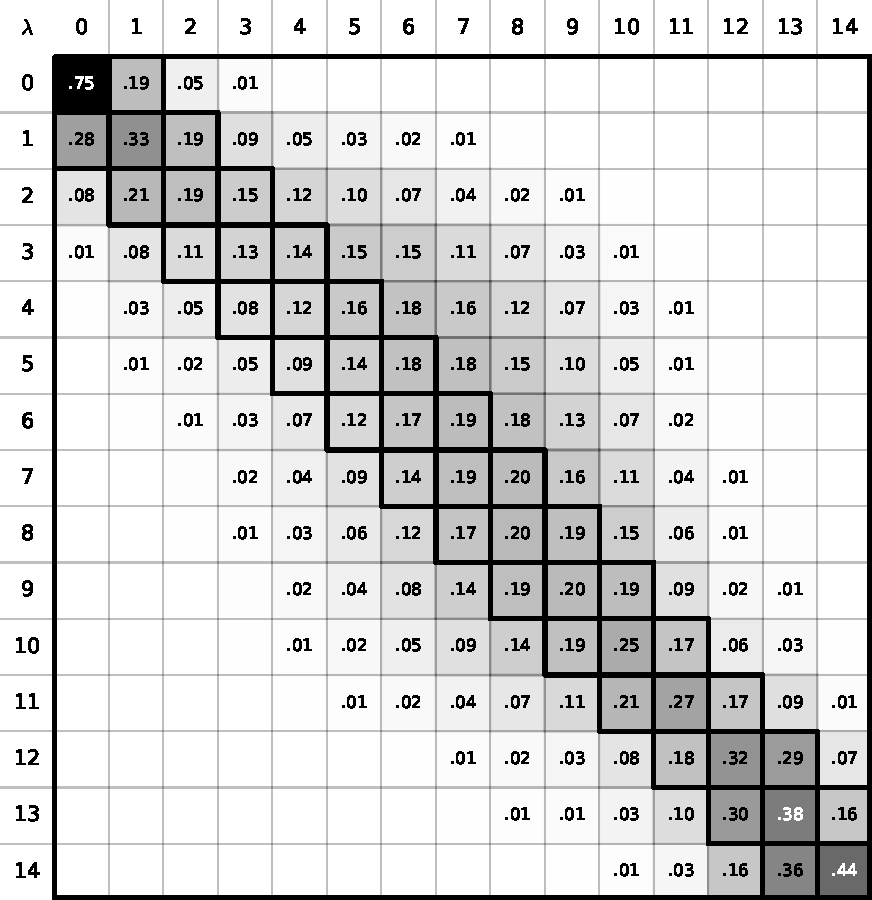
\includegraphics[width=.42\textwidth]{Figures/ohex_pyr} }}%
	\qquad
	[b]{{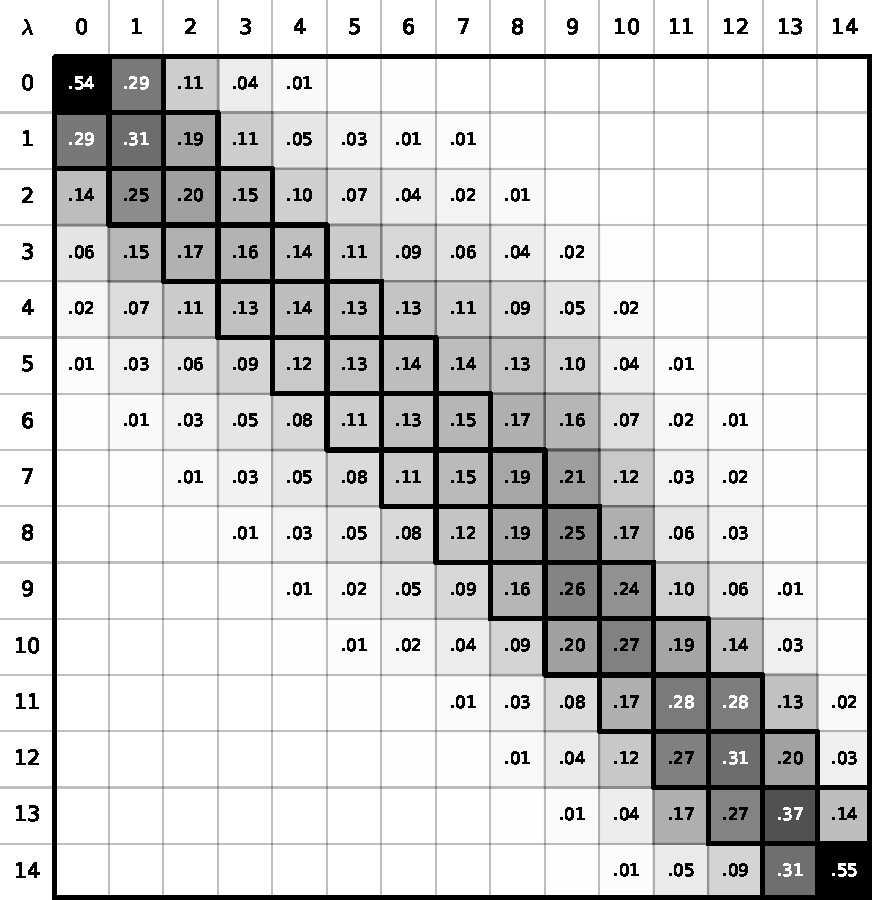
\includegraphics[width=.42\textwidth]{Figures/ohex_phen} }}%
	\qquad
	[c]{{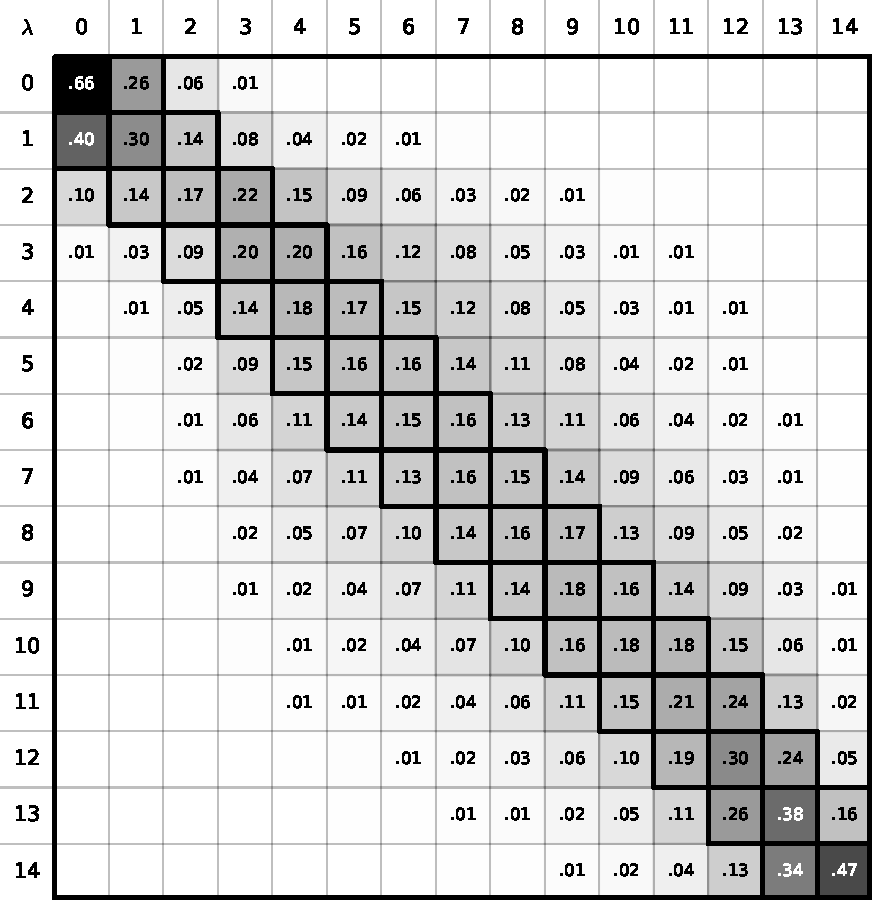
\includegraphics[width=.42\textwidth]{Figures/ooct_prop} }}%
	\qquad
	[d]{{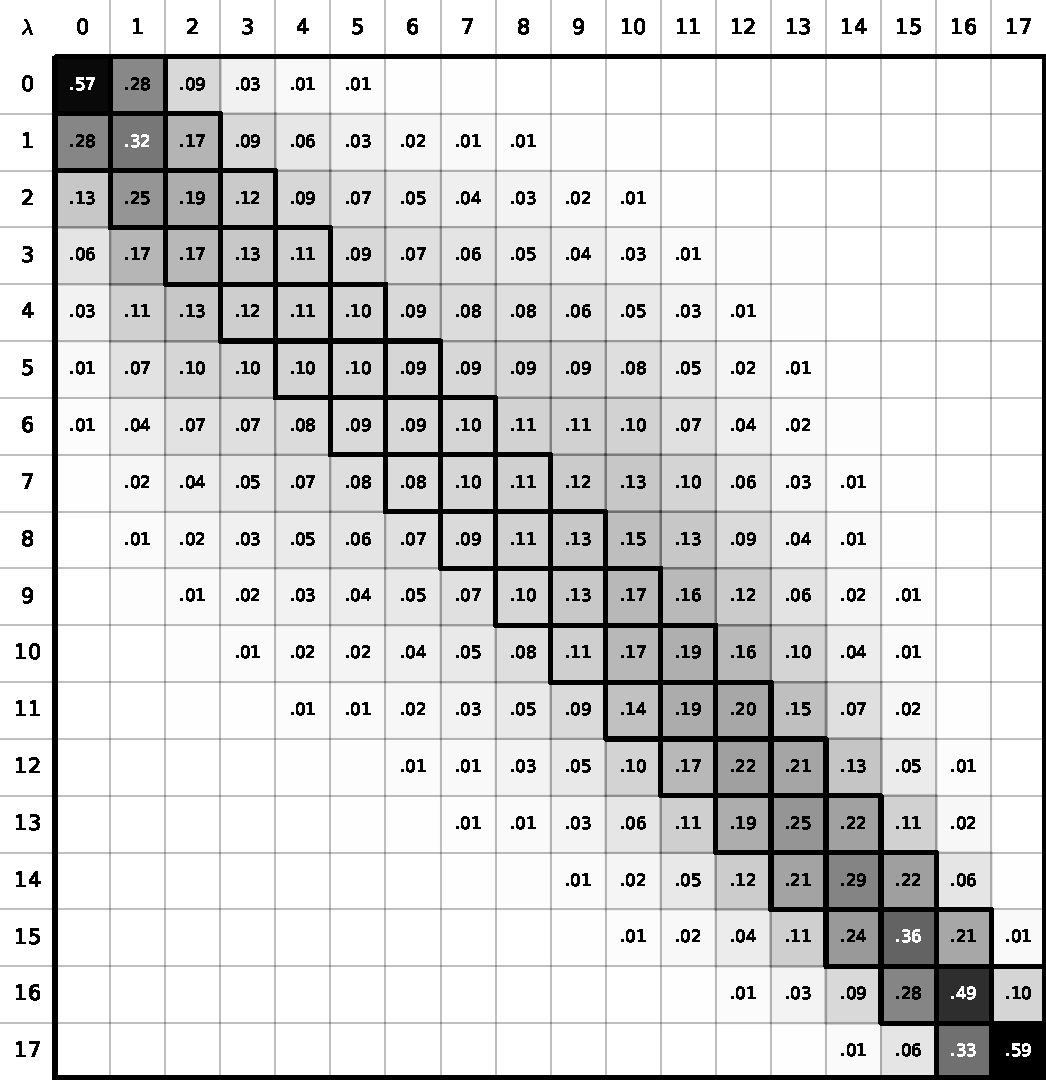
\includegraphics[width=.42\textwidth]{Figures/ooct_ant} }}%	
	[e]{{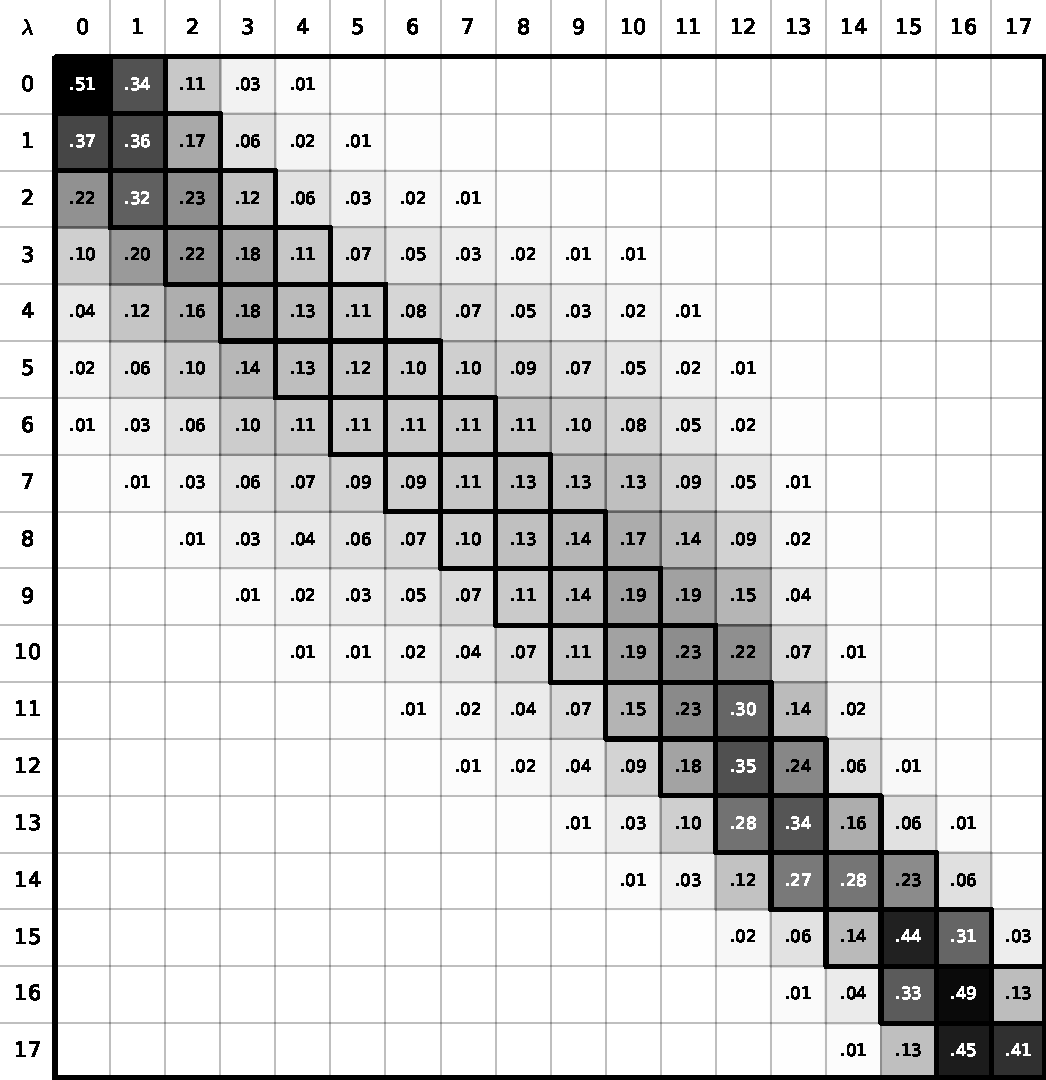
\includegraphics[width=.42\textwidth]{Figures/ooct_phen} }}%
	\qquad
	[f]{{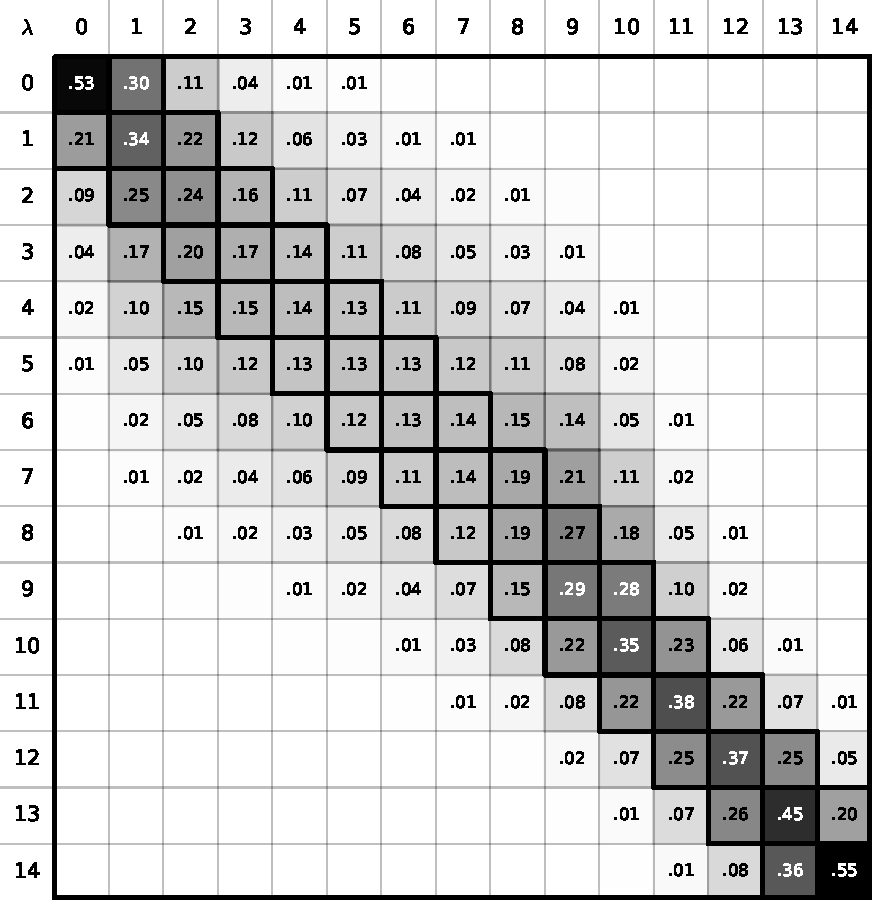
\includegraphics[width=.42\textwidth]{Figures/otol_pyr} }}%
	\qquad	
	\caption{Overlap matrix for hexane+pyrene [a], hexane+phenanthrene [b], 1-octanol+propane [c], 1-octanol+anthracene [d], 1-octanol+phenanthrene [e], and toluene+pyrene [f].}%
	\label{fig:over1}%
\end{figure}


\begin{figure}
	\centering
	[a]{{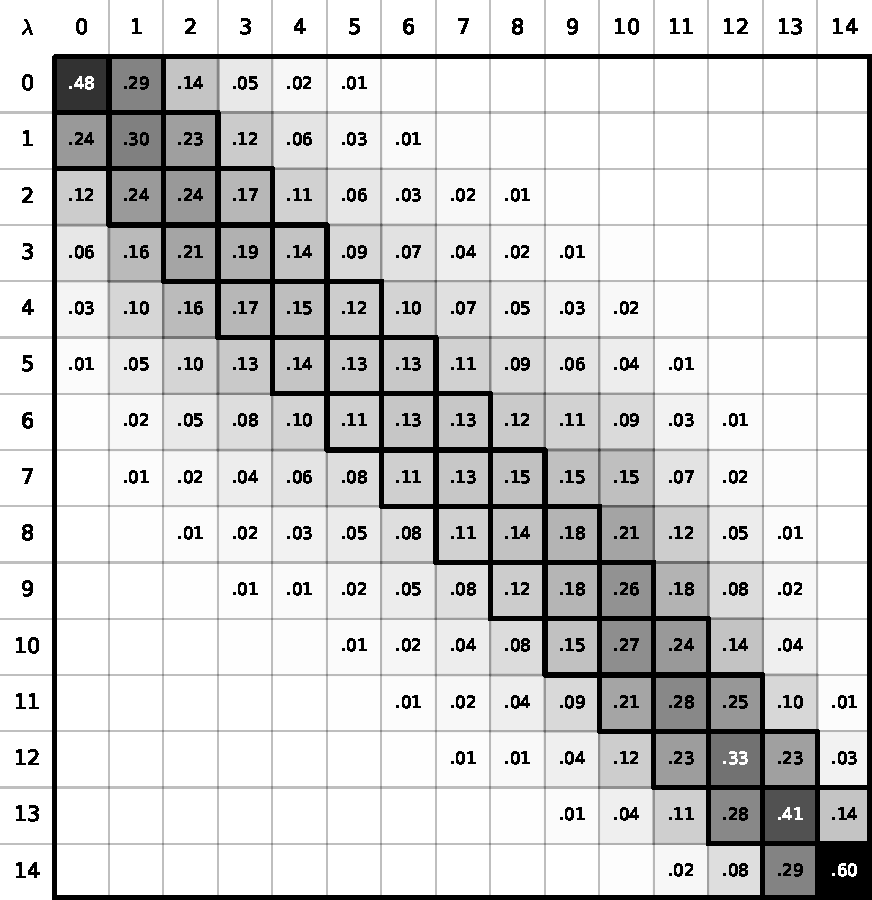
\includegraphics[width=.42\textwidth]{Figures/otol_antr} }}%
	\qquad
	[b]{{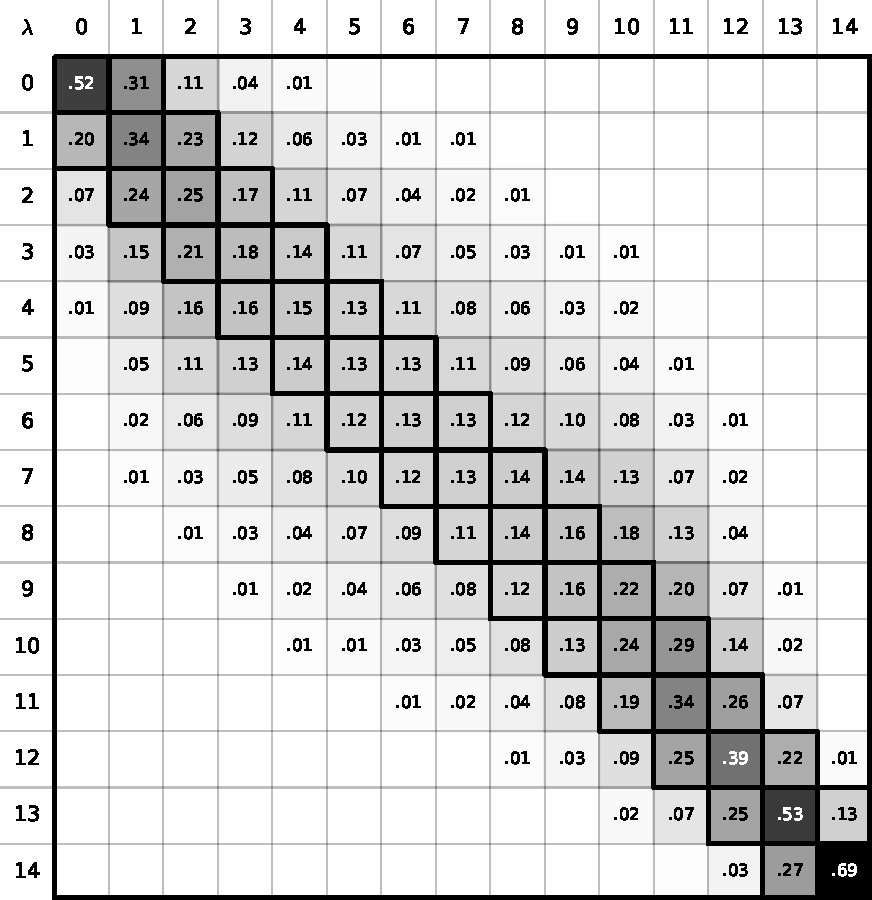
\includegraphics[width=.42\textwidth]{Figures/otol_phen} }}%	
	\qquad
	[c]{{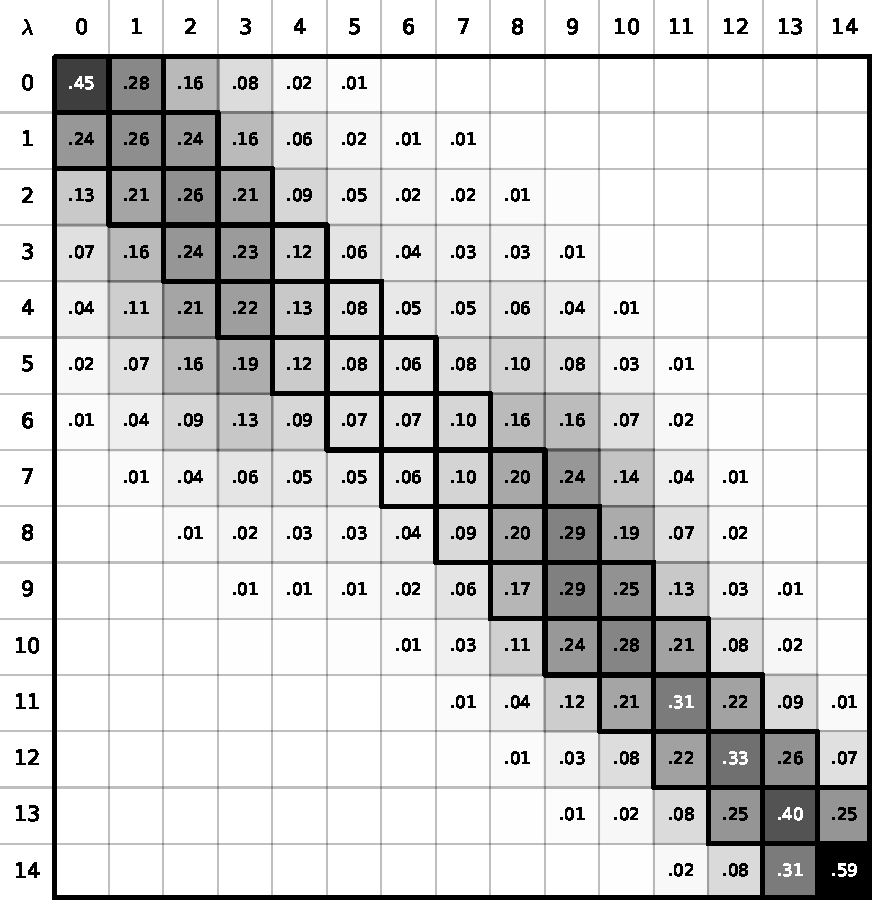
\includegraphics[width=.42\textwidth]{Figures/owat_prop} }}%
	\qquad
	[d]{{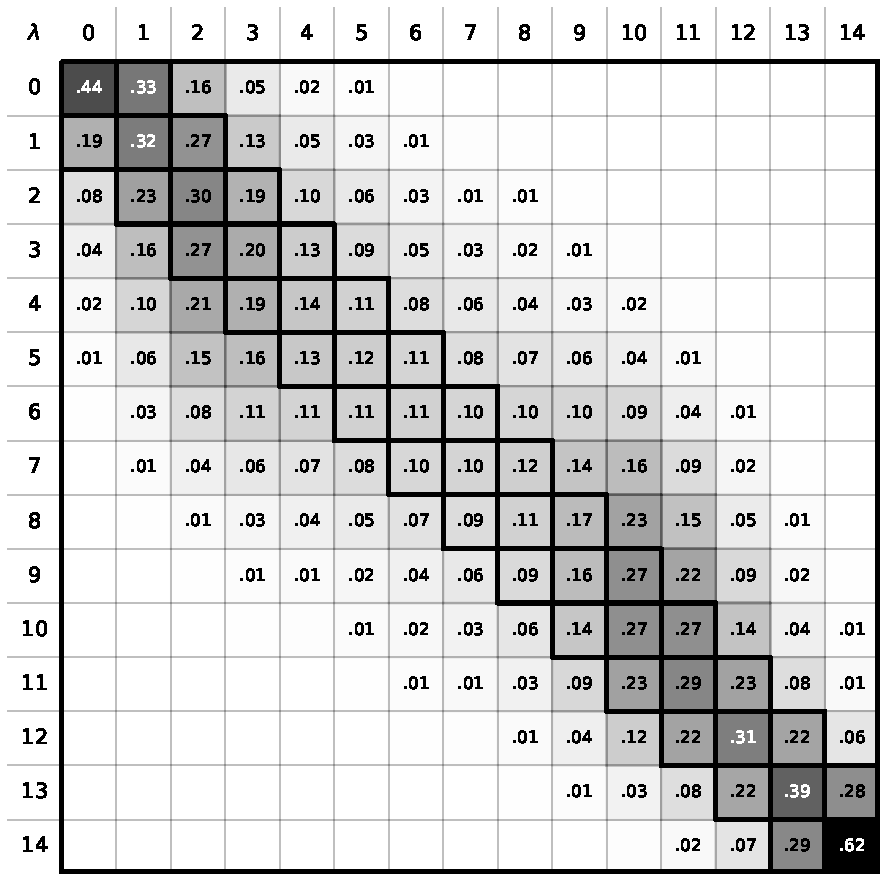
\includegraphics[width=.42\textwidth]{Figures/owat_benz} }}%
	\qquad
	[e]{{\includegraphics[width=.42\textwidth]{Figures/owat_tol} }}%
	\qquad
	[f]{{\includegraphics[width=.42\textwidth]{Figures/owat_phen} }}%	
	\caption{Overlap matrix for toluene+anthracene [a], toluene+phenanthrene [b], water+propane [c],  water+benzene [d], water+toluene [e], and water+phenanthrene [f] .}%
	\label{fig:over2}%
\end{figure}

\begin{figure}
	\centering
	[a]{{\includegraphics[width=.44\textwidth]{Figures/otolco2_1} }}%
	\qquad
	[b]{{\includegraphics[width=.44\textwidth]{Figures/otolco2_2} }}%
	\qquad
	[c]{{\includegraphics[width=.44\textwidth]{Figures/otolco2_3} }}%
	\qquad
	[d]{{\includegraphics[width=.44\textwidth]{Figures/otolco2_4} }}%		
	\caption{Overlap matrix for the different $w_{CO_2}$ of the mixture toluene+$CO_{2}$+phenanthrene. $w_{CO_2}=0.087$ [a], $w_{CO_2}=0.119$ [b], $w_{CO_2}=0.169$ [c], and $w_{CO_2}=0.289$ [d].}%
	\label{fig:over3}%
\end{figure}

%DIF < \chapter{Work Published in Scientific Conference}
\DIFaddbegin \chapter{Work Published in Scientific Conference}
\DIFaddend %
%DIF < \includepdf[pages={1-}]{C089.pdf}
\DIFaddbegin \includepdf[pages={1-}]{C089.pdf}
\DIFaddend %
%DIF < \chapter{Paper for Publication in Scientific Journal}
\DIFaddbegin \chapter{Paper for Publication in Scientific Journal}
\DIFaddend %
%DIF < \includepdf[pages={1-}]{article/elsarticle-template}
\DIFaddbegin \includepdf[pages={1-}]{article/elsarticle-template}
\DIFaddend \end{apendicesenv}
% ---


% ----------------------------------------------------------
% Anexos
% ----------------------------------------------------------

% ---
% Inicia os anexos
%% ---
%\begin{anexosenv}
%
%% Imprime uma página indicando o início dos anexos
%\partanexos
%
%% ---
%\chapter{Morbi ultrices rutrum lorem.}
%% ---
%
%% ---
%\chapter{Fusce facilisis lacinia dui}
%% ---
%
%\end{anexosenv}

%---------------------------------------------------------------------
% INDICE REMISSIVO
%---------------------------------------------------------------------
\phantompart
\printindex
%---------------------------------------------------------------------

\end{document}
